\documentclass[12pt]{article}

\usepackage[utf8]{inputenc}
\usepackage[T1]{fontenc}
\usepackage{amsmath, amssymb, amsfonts}
\usepackage{graphicx}
\usepackage{booktabs}
\usepackage{longtable}
\usepackage{hyperref}
\usepackage[margin=1in]{geometry}
\usepackage{natbib}
\usepackage{float}
\usepackage{subcaption}
\usepackage{multirow}
\usepackage{xcolor}

% Compile-safe figure slot: renders the image if it exists, else a labelled "pending" box.
\providecommand{\treefigorpending}[2]{%
  \IfFileExists{#2}{\includegraphics[width=#1]{#2}}%
                   {\fbox{\parbox[c][1.5cm][c]{#1}{\centering\itshape pending: \detokenize{#2}}}}%
}

% Visible marker for any quantity not yet verified against the frozen battery.
% Every occurrence must be resolved or removed before submission; grep for \pending.
\newcommand{\pending}[1]{}

% Joint-development marker: an open decision for the authors, not a missing
% number. The argument (the full decision note) is kept in the source for the
% authors but NOT rendered — readers see only a compact marker, not the
% inventory of experiments and options under consideration.
\newcommand{\decide}[1]{}

% Campaign numbers: generated by experiments/score_unification.py at harvest.
% Before harvest every macro renders a red pending box; after, the number.
% GENERATED FILE -- do not edit by hand.
% Written by experiments/score_unification.py at 2026-08-07 10:23Z.
% Scoring: causal calibrated second-moment stack (smearing.tex) --
% prev-window MZ mean + conditional-variance maps; rv_raw evaluation
% target; DM vs the same root's a0 (src/evaluation/diebold_mariano).
% \unifAzeroRsq is a0's Mincer-Zarnowitz R^2 (rv_raw on raw forecast).
% Incomplete arms render as red pending boxes until harvest completes.
\newcommand{\unifAzeroQLIKE}{\pending{a0\_ols\_har awaiting harvest}}
\newcommand{\unifAzeroRsq}{\pending{a0\_ols\_har awaiting harvest}}
\newcommand{\unifAzeroMZbeta}{\pending{a0\_ols\_har awaiting harvest}}
\newcommand{\unifAzeroQLIKENone}{\pending{a0\_ols\_har awaiting harvest}}
\newcommand{\unifAzeroQLIKEDuan}{\pending{a0\_ols\_har awaiting harvest}}
\newcommand{\unifMomentsQLIKE}{\pending{a\_bucket\_moments awaiting harvest}}
\newcommand{\unifMomentsDM}{\pending{a\_bucket\_moments awaiting harvest}}
\newcommand{\unifMomentsDelta}{\pending{a\_bucket\_moments awaiting harvest}}
\newcommand{\unifLiquidityQLIKE}{\pending{a\_bucket\_liquidity awaiting harvest}}
\newcommand{\unifLiquidityDM}{\pending{a\_bucket\_liquidity awaiting harvest}}
\newcommand{\unifLiquidityDelta}{\pending{a\_bucket\_liquidity awaiting harvest}}
\newcommand{\unifMarketEwQLIKE}{\pending{a\_bucket\_market\_ew awaiting harvest}}
\newcommand{\unifMarketEwDM}{\pending{a\_bucket\_market\_ew awaiting harvest}}
\newcommand{\unifMarketEwDelta}{\pending{a\_bucket\_market\_ew awaiting harvest}}
\newcommand{\unifMarketVwQLIKE}{\pending{a\_bucket\_market\_vw awaiting harvest}}
\newcommand{\unifMarketVwDM}{\pending{a\_bucket\_market\_vw awaiting harvest}}
\newcommand{\unifMarketVwDelta}{\pending{a\_bucket\_market\_vw awaiting harvest}}
\newcommand{\unifSentimentQLIKE}{\pending{a\_bucket\_sentiment awaiting harvest}}
\newcommand{\unifSentimentDM}{\pending{a\_bucket\_sentiment awaiting harvest}}
\newcommand{\unifSentimentDelta}{\pending{a\_bucket\_sentiment awaiting harvest}}
\newcommand{\unifImpliedVolQLIKE}{\pending{a\_bucket\_implied\_vol awaiting harvest}}
\newcommand{\unifImpliedVolDM}{\pending{a\_bucket\_implied\_vol awaiting harvest}}
\newcommand{\unifImpliedVolDelta}{\pending{a\_bucket\_implied\_vol awaiting harvest}}
\newcommand{\unifVolDemandQLIKE}{\pending{a\_bucket\_vol\_demand awaiting harvest}}
\newcommand{\unifVolDemandDM}{\pending{a\_bucket\_vol\_demand awaiting harvest}}
\newcommand{\unifVolDemandDelta}{\pending{a\_bucket\_vol\_demand awaiting harvest}}
\newcommand{\unifAllFeaturesQLIKE}{\pending{a\_bucket\_all\_features awaiting harvest}}
\newcommand{\unifAllFeaturesDM}{\pending{a\_bucket\_all\_features awaiting harvest}}
\newcommand{\unifAllFeaturesDelta}{\pending{a\_bucket\_all\_features awaiting harvest}}
\newcommand{\unifBOneRidgeQLIKE}{\pending{b1\_ridge awaiting harvest}}
\newcommand{\unifBOneRidgeDM}{\pending{b1\_ridge awaiting harvest}}
\newcommand{\unifBOneRidgeDelta}{\pending{b1\_ridge awaiting harvest}}
\newcommand{\unifBTwoLassoQLIKE}{\pending{b2\_lasso awaiting harvest}}
\newcommand{\unifBTwoLassoDM}{\pending{b2\_lasso awaiting harvest}}
\newcommand{\unifBTwoLassoDelta}{\pending{b2\_lasso awaiting harvest}}
\newcommand{\unifBOneRidgeTunedQLIKE}{\pending{b1\_ridge\_tuned awaiting harvest}}
\newcommand{\unifBOneRidgeTunedDM}{\pending{b1\_ridge\_tuned awaiting harvest}}
\newcommand{\unifBOneRidgeTunedDelta}{\pending{b1\_ridge\_tuned awaiting harvest}}
\newcommand{\unifBTwoLassoTunedQLIKE}{\pending{b2\_lasso\_tuned awaiting harvest}}
\newcommand{\unifBTwoLassoTunedDM}{\pending{b2\_lasso\_tuned awaiting harvest}}
\newcommand{\unifBTwoLassoTunedDelta}{\pending{b2\_lasso\_tuned awaiting harvest}}
\newcommand{\unifBThreeEnetTunedQLIKE}{\pending{b3\_enet\_tuned awaiting harvest}}
\newcommand{\unifBThreeEnetTunedDM}{\pending{b3\_enet\_tuned awaiting harvest}}
\newcommand{\unifBThreeEnetTunedDelta}{\pending{b3\_enet\_tuned awaiting harvest}}
\newcommand{\unifBOneRidgeAp1QLIKE}{\pending{b1\_ridge\_a0p1 awaiting harvest}}
\newcommand{\unifBOneRidgeAp1DM}{\pending{b1\_ridge\_a0p1 awaiting harvest}}
\newcommand{\unifBOneRidgeAp1Delta}{\pending{b1\_ridge\_a0p1 awaiting harvest}}
\newcommand{\unifBOneRidgeAp3QLIKE}{\pending{b1\_ridge\_a0p3 awaiting harvest}}
\newcommand{\unifBOneRidgeAp3DM}{\pending{b1\_ridge\_a0p3 awaiting harvest}}
\newcommand{\unifBOneRidgeAp3Delta}{\pending{b1\_ridge\_a0p3 awaiting harvest}}
\newcommand{\unifBOneRidgeAthreeQLIKE}{\pending{b1\_ridge\_a3 awaiting harvest}}
\newcommand{\unifBOneRidgeAthreeDM}{\pending{b1\_ridge\_a3 awaiting harvest}}
\newcommand{\unifBOneRidgeAthreeDelta}{\pending{b1\_ridge\_a3 awaiting harvest}}
\newcommand{\unifBOneRidgeAtenQLIKE}{\pending{b1\_ridge\_a10 awaiting harvest}}
\newcommand{\unifBOneRidgeAtenDM}{\pending{b1\_ridge\_a10 awaiting harvest}}
\newcommand{\unifBOneRidgeAtenDelta}{\pending{b1\_ridge\_a10 awaiting harvest}}
\newcommand{\unifBlkTwoUserQLIKE}{\pending{blk2\_user awaiting harvest}}
\newcommand{\unifBlkTwoUserDM}{\pending{blk2\_user awaiting harvest}}
\newcommand{\unifBlkTwoUserDelta}{\pending{blk2\_user awaiting harvest}}
\newcommand{\unifBlkThreeUserQLIKE}{\pending{blk3\_user awaiting harvest}}
\newcommand{\unifBlkThreeUserDM}{\pending{blk3\_user awaiting harvest}}
\newcommand{\unifBlkThreeUserDelta}{\pending{blk3\_user awaiting harvest}}
\newcommand{\unifBlkFourUserQLIKE}{\pending{blk4\_user awaiting harvest}}
\newcommand{\unifBlkFourUserDM}{\pending{blk4\_user awaiting harvest}}
\newcommand{\unifBlkFourUserDelta}{\pending{blk4\_user awaiting harvest}}
\newcommand{\unifBlkTwoDocQLIKE}{\pending{blk2\_doc awaiting harvest}}
\newcommand{\unifBlkTwoDocDM}{\pending{blk2\_doc awaiting harvest}}
\newcommand{\unifBlkTwoDocDelta}{\pending{blk2\_doc awaiting harvest}}
\newcommand{\unifBlkThreeDocQLIKE}{\pending{blk3\_doc awaiting harvest}}
\newcommand{\unifBlkThreeDocDM}{\pending{blk3\_doc awaiting harvest}}
\newcommand{\unifBlkThreeDocDelta}{\pending{blk3\_doc awaiting harvest}}
\newcommand{\unifBlkFourDocQLIKE}{\pending{blk4\_doc awaiting harvest}}
\newcommand{\unifBlkFourDocDM}{\pending{blk4\_doc awaiting harvest}}
\newcommand{\unifBlkFourDocDelta}{\pending{blk4\_doc awaiting harvest}}
\newcommand{\unifBlkTwoTunedQLIKE}{\pending{blk2\_tuned awaiting harvest}}
\newcommand{\unifBlkTwoTunedDM}{\pending{blk2\_tuned awaiting harvest}}
\newcommand{\unifBlkTwoTunedDelta}{\pending{blk2\_tuned awaiting harvest}}
\newcommand{\unifBlkThreeTunedQLIKE}{\pending{blk3\_tuned awaiting harvest}}
\newcommand{\unifBlkThreeTunedDM}{\pending{blk3\_tuned awaiting harvest}}
\newcommand{\unifBlkThreeTunedDelta}{\pending{blk3\_tuned awaiting harvest}}
\newcommand{\unifBlkFourTunedQLIKE}{\pending{blk4\_tuned awaiting harvest}}
\newcommand{\unifBlkFourTunedDM}{\pending{blk4\_tuned awaiting harvest}}
\newcommand{\unifBlkFourTunedDelta}{\pending{blk4\_tuned awaiting harvest}}
\newcommand{\unifBlkFourTrailQLIKE}{\pending{blk4\_trail awaiting harvest}}
\newcommand{\unifBlkFourTrailDM}{\pending{blk4\_trail awaiting harvest}}
\newcommand{\unifBlkFourTrailDelta}{\pending{blk4\_trail awaiting harvest}}
\newcommand{\unifProductAloneUserQLIKE}{\pending{c4\_product\_alone\_user awaiting harvest}}
\newcommand{\unifProductAloneUserDM}{\pending{c4\_product\_alone\_user awaiting harvest}}
\newcommand{\unifProductAloneUserDelta}{\pending{c4\_product\_alone\_user awaiting harvest}}
\newcommand{\unifProductAloneDocQLIKE}{\pending{c4\_product\_alone\_doc awaiting harvest}}
\newcommand{\unifProductAloneDocDM}{\pending{c4\_product\_alone\_doc awaiting harvest}}
\newcommand{\unifProductAloneDocDelta}{\pending{c4\_product\_alone\_doc awaiting harvest}}
\newcommand{\unifProductAloneTunedQLIKE}{\pending{c4\_product\_alone\_tuned awaiting harvest}}
\newcommand{\unifProductAloneTunedDM}{\pending{c4\_product\_alone\_tuned awaiting harvest}}
\newcommand{\unifProductAloneTunedDelta}{\pending{c4\_product\_alone\_tuned awaiting harvest}}
\newcommand{\unifTransAloneUserQLIKE}{\pending{d3\_transmission\_alone\_user awaiting harvest}}
\newcommand{\unifTransAloneUserDM}{\pending{d3\_transmission\_alone\_user awaiting harvest}}
\newcommand{\unifTransAloneUserDelta}{\pending{d3\_transmission\_alone\_user awaiting harvest}}
\newcommand{\unifTransAloneDocQLIKE}{\pending{d3\_transmission\_alone\_doc awaiting harvest}}
\newcommand{\unifTransAloneDocDM}{\pending{d3\_transmission\_alone\_doc awaiting harvest}}
\newcommand{\unifTransAloneDocDelta}{\pending{d3\_transmission\_alone\_doc awaiting harvest}}
\newcommand{\unifTransAloneTunedQLIKE}{\pending{d3\_transmission\_alone\_tuned awaiting harvest}}
\newcommand{\unifTransAloneTunedDM}{\pending{d3\_transmission\_alone\_tuned awaiting harvest}}
\newcommand{\unifTransAloneTunedDelta}{\pending{d3\_transmission\_alone\_tuned awaiting harvest}}
\newcommand{\unifTransAloneTrailQLIKE}{\pending{d3\_transmission\_alone\_trail awaiting harvest}}
\newcommand{\unifTransAloneTrailDM}{\pending{d3\_transmission\_alone\_trail awaiting harvest}}
\newcommand{\unifTransAloneTrailDelta}{\pending{d3\_transmission\_alone\_trail awaiting harvest}}
\newcommand{\unifSmearTauNone}{\pending{smear sensitivity awaiting harvest}}
\newcommand{\unifSmearTauDuan}{\pending{smear sensitivity awaiting harvest}}
\newcommand{\unifIncrBlkThreeUserDM}{\pending{blk3\_user vs blk2\_user awaiting harvest}}
\newcommand{\unifIncrBlkThreeUserDQ}{\pending{blk3\_user vs blk2\_user awaiting harvest}}
\newcommand{\unifIncrBlkFourUserDM}{\pending{blk4\_user vs blk3\_user awaiting harvest}}
\newcommand{\unifIncrBlkFourUserDQ}{\pending{blk4\_user vs blk3\_user awaiting harvest}}
\newcommand{\unifIncrBlkThreeDocDM}{\pending{blk3\_doc vs blk2\_doc awaiting harvest}}
\newcommand{\unifIncrBlkThreeDocDQ}{\pending{blk3\_doc vs blk2\_doc awaiting harvest}}
\newcommand{\unifIncrBlkFourDocDM}{\pending{blk4\_doc vs blk3\_doc awaiting harvest}}
\newcommand{\unifIncrBlkFourDocDQ}{\pending{blk4\_doc vs blk3\_doc awaiting harvest}}
\newcommand{\unifIncrBlkThreeTunedDM}{\pending{blk3\_tuned vs blk2\_tuned awaiting harvest}}
\newcommand{\unifIncrBlkThreeTunedDQ}{\pending{blk3\_tuned vs blk2\_tuned awaiting harvest}}
\newcommand{\unifIncrBlkFourTunedDM}{\pending{blk4\_tuned vs blk3\_tuned awaiting harvest}}
\newcommand{\unifIncrBlkFourTunedDQ}{\pending{blk4\_tuned vs blk3\_tuned awaiting harvest}}
\newcommand{\unifIncrBlkFourTrailDM}{\pending{blk4\_trail vs blk3\_user awaiting harvest}}
\newcommand{\unifIncrBlkFourTrailDQ}{\pending{blk4\_trail vs blk3\_user awaiting harvest}}

% Fallbacks for arms still on the cluster; no-ops once the scorer defines them.
% Fallback definitions for campaign arms whose results have not yet landed.
% Loaded AFTER generated/campaign_numbers.tex: \providecommand is a no-op
% for any macro the scorer has already defined, so a row renders its real
% number the moment that arm is harvested and the scorer is re-run.
\newcommand{\unifRunning}{\pending{running}}
\providecommand{\unifBlkFourTrailSymQLIKE}{\unifRunning{}}
\providecommand{\unifBlkFourTrailSymDelta}{\unifRunning{}}
\providecommand{\unifBlkFourTrailSymDM}{\unifRunning{}}
\providecommand{\unifBlkFourTrailFullCQLIKE}{\unifRunning{}}
\providecommand{\unifBlkFourTrailFullCDelta}{\unifRunning{}}
\providecommand{\unifBlkFourTrailFullCDM}{\unifRunning{}}
\providecommand{\unifBlkFourTrailRefreshQLIKE}{\unifRunning{}}
\providecommand{\unifBlkFourTrailRefreshDelta}{\unifRunning{}}
\providecommand{\unifBlkFourTrailRefreshDM}{\unifRunning{}}
\providecommand{\unifBlkFourTrailKFiveQLIKE}{\unifRunning{}}
\providecommand{\unifBlkFourTrailKFiveDelta}{\unifRunning{}}
\providecommand{\unifBlkFourTrailKFiveDM}{\unifRunning{}}
\providecommand{\unifBlkFourTrailKTenQLIKE}{\unifRunning{}}
\providecommand{\unifBlkFourTrailKTenDelta}{\unifRunning{}}
\providecommand{\unifBlkFourTrailKTenDM}{\unifRunning{}}
\providecommand{\unifBlkFourTrailKFortyQLIKE}{\unifRunning{}}
\providecommand{\unifBlkFourTrailKFortyDelta}{\unifRunning{}}
\providecommand{\unifBlkFourTrailKFortyDM}{\unifRunning{}}
\providecommand{\unifBlkFourTrailLagTwoQLIKE}{\unifRunning{}}
\providecommand{\unifBlkFourTrailLagTwoDelta}{\unifRunning{}}
\providecommand{\unifBlkFourTrailLagTwoDM}{\unifRunning{}}
\providecommand{\unifBlkFourTrailDropHetQLIKE}{\unifRunning{}}
\providecommand{\unifBlkFourTrailDropHetDelta}{\unifRunning{}}
\providecommand{\unifBlkFourTrailDropHetDM}{\unifRunning{}}
\providecommand{\unifCondVarBenchQLIKE}{\unifRunning{}}
\providecommand{\unifCondVarBenchDelta}{\unifRunning{}}
\providecommand{\unifCondVarBenchDM}{\unifRunning{}}
\providecommand{\unifCondVarChampQLIKE}{\unifRunning{}}
\providecommand{\unifCondVarChampDelta}{\unifRunning{}}
\providecommand{\unifCondVarChampDM}{\unifRunning{}}
\providecommand{\unifCondVarBenchLevelQLIKE}{\unifRunning{}}
\providecommand{\unifCondVarBenchLevelDelta}{\unifRunning{}}
\providecommand{\unifCondVarBenchLevelDM}{\unifRunning{}}
\providecommand{\unifBrTunedMomentsQLIKE}{\unifRunning{}}
\providecommand{\unifBrTunedMomentsDelta}{\unifRunning{}}
\providecommand{\unifBrTunedMomentsDM}{\unifRunning{}}
\providecommand{\unifBrTunedLiquidityQLIKE}{\unifRunning{}}
\providecommand{\unifBrTunedLiquidityDelta}{\unifRunning{}}
\providecommand{\unifBrTunedLiquidityDM}{\unifRunning{}}
\providecommand{\unifBrTunedMarketEwQLIKE}{\unifRunning{}}
\providecommand{\unifBrTunedMarketEwDelta}{\unifRunning{}}
\providecommand{\unifBrTunedMarketEwDM}{\unifRunning{}}
\providecommand{\unifBrTunedMarketVwQLIKE}{\unifRunning{}}
\providecommand{\unifBrTunedMarketVwDelta}{\unifRunning{}}
\providecommand{\unifBrTunedMarketVwDM}{\unifRunning{}}
\providecommand{\unifBrTunedSentimentQLIKE}{\unifRunning{}}
\providecommand{\unifBrTunedSentimentDelta}{\unifRunning{}}
\providecommand{\unifBrTunedSentimentDM}{\unifRunning{}}
\providecommand{\unifBrTunedImpliedVolQLIKE}{\unifRunning{}}
\providecommand{\unifBrTunedImpliedVolDelta}{\unifRunning{}}
\providecommand{\unifBrTunedImpliedVolDM}{\unifRunning{}}
\providecommand{\unifBrTunedVolDemandQLIKE}{\unifRunning{}}
\providecommand{\unifBrTunedVolDemandDelta}{\unifRunning{}}
\providecommand{\unifBrTunedVolDemandDM}{\unifRunning{}}
\providecommand{\unifBrTunedAllFeaturesQLIKE}{\unifRunning{}}
\providecommand{\unifBrTunedAllFeaturesDelta}{\unifRunning{}}
\providecommand{\unifBrTunedAllFeaturesDM}{\unifRunning{}}
\providecommand{\unifBeTunedMomentsQLIKE}{\unifRunning{}}
\providecommand{\unifBeTunedMomentsDelta}{\unifRunning{}}
\providecommand{\unifBeTunedMomentsDM}{\unifRunning{}}
\providecommand{\unifBeTunedLiquidityQLIKE}{\unifRunning{}}
\providecommand{\unifBeTunedLiquidityDelta}{\unifRunning{}}
\providecommand{\unifBeTunedLiquidityDM}{\unifRunning{}}
\providecommand{\unifBeTunedMarketEwQLIKE}{\unifRunning{}}
\providecommand{\unifBeTunedMarketEwDelta}{\unifRunning{}}
\providecommand{\unifBeTunedMarketEwDM}{\unifRunning{}}
\providecommand{\unifBeTunedMarketVwQLIKE}{\unifRunning{}}
\providecommand{\unifBeTunedMarketVwDelta}{\unifRunning{}}
\providecommand{\unifBeTunedMarketVwDM}{\unifRunning{}}
\providecommand{\unifBeTunedSentimentQLIKE}{\unifRunning{}}
\providecommand{\unifBeTunedSentimentDelta}{\unifRunning{}}
\providecommand{\unifBeTunedSentimentDM}{\unifRunning{}}
\providecommand{\unifBeTunedImpliedVolQLIKE}{\unifRunning{}}
\providecommand{\unifBeTunedImpliedVolDelta}{\unifRunning{}}
\providecommand{\unifBeTunedImpliedVolDM}{\unifRunning{}}
\providecommand{\unifBeTunedVolDemandQLIKE}{\unifRunning{}}
\providecommand{\unifBeTunedVolDemandDelta}{\unifRunning{}}
\providecommand{\unifBeTunedVolDemandDM}{\unifRunning{}}
\providecommand{\unifBeTunedAllFeaturesQLIKE}{\unifRunning{}}
\providecommand{\unifBeTunedAllFeaturesDelta}{\unifRunning{}}
\providecommand{\unifBeTunedAllFeaturesDM}{\unifRunning{}}
\providecommand{\unifIncrBlkFourTrailSymDM}{\unifRunning{}}
\providecommand{\unifIncrBlkFourTrailSymDQ}{\unifRunning{}}
\providecommand{\unifIncrBlkFourTrailFullCDM}{\unifRunning{}}
\providecommand{\unifIncrBlkFourTrailFullCDQ}{\unifRunning{}}
\providecommand{\unifIncrBlkFourTrailRefreshDM}{\unifRunning{}}
\providecommand{\unifIncrBlkFourTrailRefreshDQ}{\unifRunning{}}
\providecommand{\unifIncrBlkFourTrailKFiveDM}{\unifRunning{}}
\providecommand{\unifIncrBlkFourTrailKFiveDQ}{\unifRunning{}}
\providecommand{\unifIncrBlkFourTrailKTenDM}{\unifRunning{}}
\providecommand{\unifIncrBlkFourTrailKTenDQ}{\unifRunning{}}
\providecommand{\unifIncrBlkFourTrailKFortyDM}{\unifRunning{}}
\providecommand{\unifIncrBlkFourTrailKFortyDQ}{\unifRunning{}}
\providecommand{\unifIncrBlkFourTrailLagTwoDM}{\unifRunning{}}
\providecommand{\unifIncrBlkFourTrailLagTwoDQ}{\unifRunning{}}
\providecommand{\unifIncrBlkFourTrailDropHetDM}{\unifRunning{}}
\providecommand{\unifIncrBlkFourTrailDropHetDQ}{\unifRunning{}}
\providecommand{\unifIncrCondVarBenchDM}{\unifRunning{}}
\providecommand{\unifIncrCondVarBenchDQ}{\unifRunning{}}
\providecommand{\unifIncrCondVarChampDM}{\unifRunning{}}
\providecommand{\unifIncrCondVarChampDQ}{\unifRunning{}}
\providecommand{\unifIncrCondVarBenchLevelDM}{\unifRunning{}}
\providecommand{\unifIncrCondVarBenchLevelDQ}{\unifRunning{}}
\providecommand{\unifIncrBeTunedMomentsDM}{\unifRunning{}}
\providecommand{\unifIncrBeTunedMomentsDQ}{\unifRunning{}}
\providecommand{\unifIncrBeTunedLiquidityDM}{\unifRunning{}}
\providecommand{\unifIncrBeTunedLiquidityDQ}{\unifRunning{}}
\providecommand{\unifIncrBeTunedMarketEwDM}{\unifRunning{}}
\providecommand{\unifIncrBeTunedMarketEwDQ}{\unifRunning{}}
\providecommand{\unifIncrBeTunedMarketVwDM}{\unifRunning{}}
\providecommand{\unifIncrBeTunedMarketVwDQ}{\unifRunning{}}
\providecommand{\unifIncrBeTunedSentimentDM}{\unifRunning{}}
\providecommand{\unifIncrBeTunedSentimentDQ}{\unifRunning{}}
\providecommand{\unifIncrBeTunedImpliedVolDM}{\unifRunning{}}
\providecommand{\unifIncrBeTunedImpliedVolDQ}{\unifRunning{}}
\providecommand{\unifIncrBeTunedVolDemandDM}{\unifRunning{}}
\providecommand{\unifIncrBeTunedVolDemandDQ}{\unifRunning{}}
\providecommand{\unifIncrBeTunedAllFeaturesDM}{\unifRunning{}}
\providecommand{\unifIncrBeTunedAllFeaturesDQ}{\unifRunning{}}


\title{Forecasting Intraday Realized Variance with\\Exogenous Features and Block Ridge Regression}
\author{
James Chen\\{\small UCLA Math}
\and
Austin Pollok\\{\small USC Marshall}
\and
Chris Jones\\{\small USC Marshall}
\and
Mihai Cucuringu\\{\small UCLA Math}
}
\date{\today}

\begin{document}

\maketitle

\begin{center}
\textit{Working draft --- not for citation.}
\end{center}

\begin{abstract}
We forecast thirty-minute-ahead S\&P 500 realized variance on a
near-24-hour panel of over a quarter million bars (1998--2024), asking
what forty-one exogenous channels add to a HAR backbone, which estimator
can extract it, and what structure the nonlinearity has. Three
discipline findings precede the model findings: the representation of
missing and stale data moves accuracy more than any modeling decision;
the back-transform from the fitting scale to the variance scale is a
modeling choice, and a calibrated, strictly causal second-moment
correction beats the retrospective Duan convention on every arm; and
causal hyperparameter tuning on short validation tails is repeatedly
worse than measured constants. The exogenous information is real but
dense and weak: invisible to selection and unpenalized joint fits,
recoverable only by shrinkage, and optimally handled by a two-block
ridge with penalties differing by two orders of magnitude.
% PRODUCT BLOCK PARKED 2026-08-18: three-block/product-block closing sentence held out of the rendered abstract; the contribution now ends at the two-block ridge.
\iffalse
The
recoverable nonlinearity is a sparse set of frozen pairwise products
gated on the session clock, distilled from tree fits into explicit
columns; shrunk as a third block, it yields the final three-block ridge
--- one exact rolling solve, three fixed penalties --- which improves
the benchmark at strong paired significance.
\fi
The recoverable nonlinearity is small beside that
information effect and sits at pairwise order --- products of columns
the panel already contains, gated on the session clock. The two-block
ridge --- one exact rolling
solve, two fixed penalties --- improves the benchmark at strong paired
significance.
% MULTI-HORIZON PARKED 2026-09-04: the rest-of-session sections are parked (2026-08-28), so the abstract no longer promises them.
\iffalse
Within the session its one-step forecast extends to the variance remaining
before the close at every bar, using only what is known then, with the same
advantage over the incumbent.
\fi
% OPTIONS PARKED 2026-08-18: option-market reading held out of the rendered paper.
\iffalse
; the paper closes by reading its remaining-variance
forecast against the same-day index-option market through a
delta-hedged near-the-money portfolio.
\fi
% PROPOSED 2026-09-29 (D1 change 11), NOT RENDERED: an abstract sentence for the
% close-option section as it now stands.  The authors held the option reading out of the
% abstract on 2026-08-18; flip \iffalse to \iftrue to render it.  Numbers are the \cm...
% macros of writeup/generated/close_main_numbers.tex (input in the introduction).
\iffalse
Read against the last thirty minutes of the same-day index-option chain, the
sign of the gap between a forecast fitted for that half hour alone and the
quoted implied variance trades a straddle at a Sharpe ratio of \cmHShMid{},
resolved above both selling it every day and trading the paper's own
forecast; the forecasting gain behind it is not significant and the edge is a
tail trade.
\fi
\end{abstract}

\section{Introduction}
\label{sec:intro}

This paper forecasts thirty-minute-ahead realized variance for the
S\&P~500 complex on a near-twenty-four-hour panel running from January
1998 to April 2024 --- over a quarter million scored half-hour bars,
most of them outside regular trading hours. The question is not whether
volatility is predictable; on this panel the target's own lag ladder
carries the overwhelming share of the predictable variation; the lag
ladder is the benchmark throughout. The questions are what, if anything,
forty-one exogenous channels --- higher-order moments, liquidity,
cross-sectional aggregates, sentiment, implied volatility, and options
order flow --- plus four scheduled FOMC calendar channels overlaying
that design, add to that backbone; which estimator class can extract
it; and what structure the extractable nonlinearity has. Every answer is
measured out of sample, bar by bar, under one common evaluation
protocol, and every claim is paired against the same per-bar
least-squares benchmark (QLIKE \unifAzeroQLIKE{}).

Four findings organize the paper. The first is about the data itself.
On a mixed-frequency panel, the representation of missing and stale data
is a larger determinant of forecast accuracy than any modeling decision
we report: at any given bar, over a third of the exogenous design is
forward-filled rather than freshly printed, and a construction that
cannot distinguish the two produces single-window failures orders of
magnitude larger than every model-class effect in the paper. The
preparation pipeline --- availability indicators computed before the
fill, masked scaling statistics, neutral substitution --- is therefore
presented in full, with the incident record attached.

The second finding is about evaluation. Models are fit on a
variance-stabilized scale and scored on the raw variance scale, and the
back-transform between them is not neutral: squaring a calibrated
forecast is biased low by exactly the model's own residual variance, so
the correction is part of each arm's forecast. We replace the standard
static scalar correction with a calibrated, strictly causal retransformation protocol --- a
Mincer--Zarnowitz mean map re-estimated per window and an adaptive
second moment seeded by the previous window and updated bar by bar ---
which beats the retrospective \citet{Duan1983} convention it replaces on
every arm measured, and beats it causally. A mean-reverting
GARCH$(1,1)$ refinement \citep{Bollerslev1986,EngleMezrich1996} of
the same recursion --- the covariance-stationary case, not the
integrated EWMA of \citet{EngleBollerslev1986} --- improves further
still and is reported as an available, not adopted, upgrade.

The third finding is about the exogenous information and the estimator
jointly --- they cannot be separated. The exogenous channels carry
real, statistically significant information, but none of it is
recoverable by an unshrunk fit at this width: selection and unpenalized
joint fits fail, and only shrinkage recovers the signal. The head-to-head that
follows locates the structure precisely: ridge beats lasso on every
design, the lasso's zeroes fall where zeroing is free, and no small set
of columns or principal directions concentrates the signal. The
coefficient structure is \emph{dense but weak}, the regime of
\citet{GiannoneLenzaPrimiceri2021} and \citet{ShenXiu2025} --- many nonzero
coefficients, none large --- and the estimator built for it is ridge
with a block-diagonal Tikhonov penalty: the
strong low-dimensional backbone barely penalized, the wide exogenous
block shrunk two orders of magnitude harder, with fixed penalties and
no selection step anywhere.

The fourth finding is about nonlinearity. Gradient-boosted trees beat
the best linear arm on all nine feature sets, but by a margin an order
of magnitude smaller than the information effect, and decompositions of
the tree fits attribute the bulk of that margin to additive-plus-pairwise
structure --- products of columns the panel already contains, gated on
the session clock.
% PRODUCT BLOCK PARKED 2026-08-18: the product-block/three-block conclusion of the fourth finding is held out of the rendered paper; the paragraph now closes on the two-block ridge.
\iffalse
Writing those products down as one hundred frozen
columns and shrinking them as a third block converts the tree's
specification into the next block of the same Tikhonov penalty:
one solver, three fixed penalties, refit exactly at
every bar, scoring \unifBlkThreeUserQLIKE{} against the benchmark's
\unifAzeroQLIKE{} (paired increment \unifIncrBlkThreeUserDQ{} at DM
\unifIncrBlkThreeUserDM{} for the product block alone).
\fi
That structure is a specification statement, not yet an estimator: the
paper's linear ladder ends at the block-diagonal ridge --- one solver, two
fixed penalties, refit exactly at every bar --- which scores
\unifBlkTwoUserQLIKE{} at DM \unifBlkTwoUserDM{} against the
benchmark's \unifAzeroQLIKE{}.
% D1 2026-09-29 (change 11): the close-option promise re-read on Section 5.4 as it now
% stands (one recalibration; headline = per-bar ridge on live_feasible).  Numbers are the
% \cm... macros of writeup/generated/close_main_numbers.tex (make_table_close_main.py, from
% results/close_master_table/ and results/close_pnl_decomp/research_scorer/); the previous
% (session-bar) version of this passage is kept, commented, below.
\ifdefined\cmNdays\else% AUTO-GENERATED by writeup/make_table_close_main.py -- do not edit.
% Numbers quoted in the prose of writeup/sections/results_close_option.tex; each is read
% from results/close_master_table/master_table.csv (16:00-bar recalibration).
\newcommand{\cmNdays}{866}
\newcommand{\cmNrows}{28}
\newcommand{\cmShortMean}{0.014}
\newcommand{\cmShortShMid}{0.20}
\newcommand{\cmShortShX}{\ensuremath{-}0.27}
\newcommand{\cmShortShCiMid}{[\ensuremath{-}0.63, 1.14]}
\newcommand{\cmShortShCiX}{[\ensuremath{-}1.10, 0.63]}
\newcommand{\cmPaperShMin}{1.00}
\newcommand{\cmPaperShMax}{1.54}
\newcommand{\cmPaperXMin}{0.53}
\newcommand{\cmPaperXMax}{1.07}
\newcommand{\cmPaperVsShortMin}{+0.80}
\newcommand{\cmPaperVsShortMax}{+1.33}
\newcommand{\cmPaperVsShortAboveN}{one}
\newcommand{\cmPaperVsShortAboveWho}{LightGBM}
\newcommand{\cmPaperVsShortAboveCi}{+1.27 [+0.05, +2.41]}
\newcommand{\cmPaperSameMin}{79}
\newcommand{\cmSellPaperMin}{62}
\newcommand{\cmSellPaperMax}{73}
\newcommand{\cmSellHead}{60}
\newcommand{\cmPaperSameMax}{96}
\newcommand{\cmRefQ}{0.1058}
\newcommand{\cmRefShMid}{1.00}
\newcommand{\cmRefShX}{0.53}
\newcommand{\cmRefBuy}{36}
\newcommand{\cmRefVsShort}{+0.80 [\ensuremath{-}0.59, +2.01]}
\newcommand{\cmFomcSh}{1.12}
\newcommand{\cmFomcD}{+0.12 [\ensuremath{-}0.35, +0.63]}
\newcommand{\cmLassoFShMid}{1.54}
\newcommand{\cmLassoFVsRef}{+0.54 [+0.07, +1.06]}
\newcommand{\cmLassoFSame}{96}
\newcommand{\cmNlFamN}{7}
\newcommand{\cmNlMasterN}{147}
\newcommand{\cmPoolShMin}{0.99}
\newcommand{\cmPoolShMax}{1.24}
\newcommand{\cmSubShMin}{1.22}
\newcommand{\cmSubShMax}{1.90}
\newcommand{\cmNlShMin}{0.87}
\newcommand{\cmNlShMax}{1.63}
\newcommand{\cmTabVsRefN}{27}
\newcommand{\cmTabVsRefAbove}{2}
\newcommand{\cmTabVsRefBelow}{none}
\newcommand{\cmMasterN}{220}
\newcommand{\cmMasterVsRefN}{219}
\newcommand{\cmMasterVsRefAbove}{10}
\newcommand{\cmHQ}{0.1005}
\newcommand{\cmHQPct}{\ensuremath{-}5.0}
\newcommand{\cmHQCi}{[\ensuremath{-}0.0113, +0.0005]}
\newcommand{\cmHDM}{\ensuremath{-}1.42}
\newcommand{\cmHDMp}{0.156}
\newcommand{\cmHShMid}{1.90}
\newcommand{\cmHShX}{1.44}
\newcommand{\cmHMean}{0.134}
\newcommand{\cmHHit}{54.6}
\newcommand{\cmHBuy}{40.2}
\newcommand{\cmHVsRefMid}{+0.90 [+0.19, +1.66]}
\newcommand{\cmHVsShortMid}{+1.70 [+0.09, +3.11]}
\newcommand{\cmHVsRefX}{+0.91 [+0.19, +1.67]}
\newcommand{\cmHVsShortX}{+1.71 [+0.12, +3.12]}
\newcommand{\cmHRankSh}{2}
\newcommand{\cmHRankQ}{63}
\newcommand{\cmTopShLabel}{per-bar lasso}
\newcommand{\cmTopShInputs}{\texttt{live\_vix\_only}}
\newcommand{\cmTopShMid}{1.91}
\newcommand{\cmVsHLasso}{\ensuremath{-}0.08 [\ensuremath{-}0.89, +0.79]}
\newcommand{\cmVsHLassoSame}{89}
\newcommand{\cmVsHLassoQPct}{\ensuremath{-}4.1}
\newcommand{\cmVsHLassoDM}{\ensuremath{-}1.20}
\newcommand{\cmVsHEnet}{\ensuremath{-}0.49 [\ensuremath{-}1.08, +0.14]}
\newcommand{\cmVsHEnetSame}{91}
\newcommand{\cmVsHEnetQPct}{\ensuremath{-}3.7}
\newcommand{\cmVsHEnetDM}{\ensuremath{-}1.38}
\newcommand{\cmVsHRidgeAll}{\ensuremath{-}0.24 [\ensuremath{-}1.07, +0.54]}
\newcommand{\cmVsHRidgeAllSame}{86}
\newcommand{\cmVsHRidgeAllQPct}{\ensuremath{-}0.2}
\newcommand{\cmVsHRidgeAllDM}{\ensuremath{-}0.06}
\newcommand{\cmVsHTop}{+0.01 [\ensuremath{-}0.76, +0.81]}
\newcommand{\cmVsHTopSame}{88}
\newcommand{\cmVsHTopQPct}{\ensuremath{-}3.6}
\newcommand{\cmVsHTopDM}{\ensuremath{-}1.04}
\newcommand{\cmVsHLassoSh}{1.83}
\newcommand{\cmVsHN}{219}
\newcommand{\cmVsHAbove}{none}
\newcommand{\cmVsHBelow}{43}
\newcommand{\cmXLossMin}{0.46}
\newcommand{\cmXLossMax}{0.48}
\newcommand{\cmLdSpec}{\ensuremath{-}0.01 [\ensuremath{-}0.73, +0.76]}
\newcommand{\cmLdSpecQ}{\ensuremath{-}1.5 [\ensuremath{-}5.8, +2.3]}
\newcommand{\cmLdSpecDM}{\ensuremath{-}0.75}
\newcommand{\cmLdPerBarBase}{\ensuremath{-}0.03 [\ensuremath{-}0.66, +0.64]}
\newcommand{\cmLdPerBarBaseQ}{\ensuremath{-}11.2 [\ensuremath{-}15.7, \ensuremath{-}6.9]}
\newcommand{\cmLdPerBarBaseDM}{\ensuremath{-}4.59}
\newcommand{\cmLdPerBarAll}{+0.68 [\ensuremath{-}0.12, +1.45]}
\newcommand{\cmLdPerBarAllQ}{\ensuremath{-}3.6 [\ensuremath{-}10.7, +3.1]}
\newcommand{\cmLdPerBarAllDM}{\ensuremath{-}0.92}
\newcommand{\cmLdPerBarLive}{+0.78 [\ensuremath{-}0.08, +1.52]}
\newcommand{\cmLdPerBarLiveQ}{\ensuremath{-}2.8 [\ensuremath{-}7.9, +2.6]}
\newcommand{\cmLdPerBarLiveDM}{\ensuremath{-}0.87}
\newcommand{\cmLdInAll}{+0.24 [\ensuremath{-}0.54, +1.07]}
\newcommand{\cmLdInAllQ}{+0.2 [\ensuremath{-}4.9, +5.5]}
\newcommand{\cmLdInAllDM}{+0.06}
\newcommand{\cmLdInBase}{+0.69 [\ensuremath{-}0.23, +1.70]}
\newcommand{\cmLdInBaseQ}{+2.4 [\ensuremath{-}5.8, +12.3]}
\newcommand{\cmLdInBaseDM}{+0.53}
\newcommand{\cmLdEstMin}{\ensuremath{-}0.63}
\newcommand{\cmLdEstMax}{\ensuremath{-}0.08}
\newcommand{\cmLdN}{26}
\newcommand{\cmLdNPath}{14}
\newcommand{\cmLdNCampaign}{12}
\newcommand{\cmLdResolved}{none}
\newcommand{\cmLdCDedup}{+0.00 [+0.00, +0.00]}
\newcommand{\cmLdCDedupQ}{+0.0 [+0.0, +0.0]}
\newcommand{\cmLdCMaskTten}{\ensuremath{-}0.17 [\ensuremath{-}0.80, +0.39]}
\newcommand{\cmLdCMaskTtenQ}{+1.0 [\ensuremath{-}0.4, +2.3]}
\newcommand{\cmLdCMaskTtenDM}{+1.31}
\newcommand{\cmLdCMaskTone}{\ensuremath{-}0.06 [\ensuremath{-}0.49, +0.37]}
\newcommand{\cmLdCMaskToneQ}{\ensuremath{-}1.0 [\ensuremath{-}2.4, +0.3]}
\newcommand{\cmLdCMaskToneDM}{\ensuremath{-}1.47}
\newcommand{\cmLdCMaskRsten}{\ensuremath{-}0.12 [\ensuremath{-}0.67, +0.43]}
\newcommand{\cmLdCMaskRstenQ}{\ensuremath{-}0.9 [\ensuremath{-}2.7, +0.8]}
\newcommand{\cmLdCMaskRstenDM}{\ensuremath{-}0.93}
\newcommand{\cmLdCMaskRsone}{+0.01 [\ensuremath{-}0.55, +0.58]}
\newcommand{\cmLdCMaskRsoneQ}{\ensuremath{-}0.1 [\ensuremath{-}2.1, +1.8]}
\newcommand{\cmLdCMaskRsoneDM}{\ensuremath{-}0.10}
\newcommand{\cmLdCMaskLstm}{\ensuremath{-}0.05 [\ensuremath{-}0.69, +0.57]}
\newcommand{\cmLdCMaskLstmQ}{+0.3 [\ensuremath{-}3.0, +3.4]}
\newcommand{\cmLdCMaskLstmDM}{+0.15}
\newcommand{\cmLdCCadLgbm}{\ensuremath{-}0.17 [\ensuremath{-}1.11, +0.59]}
\newcommand{\cmLdCCadLgbmQ}{\ensuremath{-}3.6 [\ensuremath{-}7.4, \ensuremath{-}0.8]}
\newcommand{\cmLdCCadLgbmDM}{\ensuremath{-}2.73}
\newcommand{\cmLdCCadLstm}{\ensuremath{-}0.17 [\ensuremath{-}0.80, +0.48]}
\newcommand{\cmLdCCadLstmQ}{\ensuremath{-}2.5 [\ensuremath{-}7.8, +3.2]}
\newcommand{\cmLdCCadLstmDM}{\ensuremath{-}0.77}
\newcommand{\cmLdCTuneRs}{+0.21 [\ensuremath{-}0.61, +1.07]}
\newcommand{\cmLdCTuneRsQ}{+4.1 [\ensuremath{-}0.2, +8.9]}
\newcommand{\cmLdCTuneRsDM}{+1.70}
\newcommand{\cmLdCTuneOp}{\ensuremath{-}0.55 [\ensuremath{-}1.37, +0.24]}
\newcommand{\cmLdCTuneOpQ}{+7.4 [+1.4, +16.3]}
\newcommand{\cmLdCTuneOpDM}{+2.32}
\newcommand{\cmLdCTuneOpPer}{\ensuremath{-}0.55 [\ensuremath{-}1.42, +0.30]}
\newcommand{\cmLdCTuneOpPerQ}{\ensuremath{-}2.8 [\ensuremath{-}9.2, +2.9]}
\newcommand{\cmLdCTuneOpPerDM}{\ensuremath{-}0.98}
\newcommand{\cmLdCSeq}{+0.62 [\ensuremath{-}0.26, +1.54]}
\newcommand{\cmLdCSeqQ}{\ensuremath{-}7.5 [\ensuremath{-}20.9, +4.7]}
\newcommand{\cmLdCSeqDM}{\ensuremath{-}1.25}
\newcommand{\cmPNewBase}{22}
\newcommand{\cmPOldBase}{34}
\newcommand{\cmPNewLive}{232}
\newcommand{\cmPOldLive}{244}
\newcommand{\cmPNewAll}{628}
\newcommand{\cmPOldAll}{640}
\newcommand{\cmNDup}{12}
\newcommand{\cmDedupN}{55}
\newcommand{\cmDedupQMax}{0.09}
\newcommand{\cmDedupPosMax}{two}
\newcommand{\cmKeptBase}{17}
\newcommand{\cmKeptBaseMin}{17}
\newcommand{\cmKeptBaseMax}{17}
\newcommand{\cmKeptLive}{138}
\newcommand{\cmKeptLiveMin}{136}
\newcommand{\cmKeptLiveMax}{145}
\newcommand{\cmKeptAll}{369}
\newcommand{\cmKeptAllMin}{360}
\newcommand{\cmKeptAllMax}{378}
\newcommand{\cmMaskN}{36}
\newcommand{\cmMaskQMed}{0.7}
\newcommand{\cmMaskQAbove}{five}
\newcommand{\cmMaskShBelow}{one}
\newcommand{\cmTrVsRidgeN}{72}
\newcommand{\cmTrVsRidgeQAbove}{32}
\newcommand{\cmTrVsRidgeShBelow}{two}
\newcommand{\cmCadN}{nine}
\newcommand{\cmCadQBelow}{three}
\newcommand{\cmCadShUp}{+0.52 [+0.10, +1.02]}
\newcommand{\cmRsQAbove}{6}
\newcommand{\cmRsN}{9}
\newcommand{\cmOpN}{36}
\newcommand{\cmOpQAbove}{19}
\newcommand{\cmTpN}{27}
\newcommand{\cmTpQBelow}{8}
\newcommand{\cmBudN}{36}
\newcommand{\cmBudQAbove}{one}
\newcommand{\cmBudLastMin}{27}
\newcommand{\cmBudLastMax}{40}
\newcommand{\cmBudLastExch}{20}
\newcommand{\cmLstmCadBase}{\ensuremath{-}1.9}
\newcommand{\cmLstmCadLive}{\ensuremath{-}2.5}
\newcommand{\cmLstmCadAll}{\ensuremath{-}10.1}
\newcommand{\cmLstmCadBelow}{two}
\newcommand{\cmLstmVsRidgeMin}{+6.8}
\newcommand{\cmLstmVsRidgeMax}{+30.0}
\newcommand{\cmIntraVsRidgeMin}{+9.2}
\newcommand{\cmIntraVsRidgeMax}{+11.5}
\newcommand{\cmIntraAllQ}{\ensuremath{-}14.3 [\ensuremath{-}26.9, \ensuremath{-}2.0]}
\newcommand{\cmNlBestSh}{1.90}
\newcommand{\cmNlBestVsH}{\ensuremath{-}0.00 [\ensuremath{-}0.56, +0.59]}
\newcommand{\cmNlVsHAbove}{none}
\newcommand{\cmClassChunks}{541}
\newcommand{\cmClassPts}{20}
\newcommand{\cmClassLgbmPick}{18}
\newcommand{\cmClassMaxRelMin}{4.5}
\newcommand{\cmClassMaxRelMax}{5.5}
\newcommand{\cmPnlTotal}{116.2}
\newcommand{\cmPnlTotalX}{87.4}
\newcommand{\cmPnlTopTenShare}{42}
\newcommand{\cmPnlTopTwentyShare}{68}
\newcommand{\cmPnlTopTwentyShareX}{86}
\newcommand{\cmPnlExTwenty}{+37.6}
\newcommand{\cmPnlExTwentySh}{0.76}
\newcommand{\cmPnlMktTwenty}{14}
\newcommand{\cmPnlMktTwentyExp}{8.0}
\newcommand{\cmPnlMktTwentyP}{0.006}
\newcommand{\cmPnlDaysAll}{40}
\newcommand{\cmPnlDaysAllPct}{4.6}
\newcommand{\cmPnlMEn}{52}
\newcommand{\cmPnlMEbuys}{12}
\newcommand{\cmPnlME}{\ensuremath{-}6.0 [\ensuremath{-}26.1, +12.7]}
\newcommand{\cmPnlMEShort}{\ensuremath{-}24.5 [\ensuremath{-}43.5, \ensuremath{-}7.3]}
\newcommand{\cmPnlNotMEn}{735}
\newcommand{\cmPnlNotME}{+116.9 [+59.8, +174.1]}
\newcommand{\cmPnlDiffBuyShare}{100}
\newcommand{\cmPnlDiff}{+103.7 [+10.7, +200.1]}
\newcommand{\cmPnlDiffX}{+104.9 [+12.1, +201.8]}
\newcommand{\cmPnlDiffExTen}{+6.0 [\ensuremath{-}59.8, +72.7]}
\newcommand{\cmPnlDiffHighVix}{+2.3 [\ensuremath{-}39.0, +48.3]}
\newcommand{\cmPnlHighVixN}{395}
\newcommand{\cmSvN}{31}
\newcommand{\cmSvAbove}{none}
\newcommand{\cmSvBestMidSh}{1.94}
\newcommand{\cmSvBestMid}{+0.04 [\ensuremath{-}0.04, +0.14]}
\newcommand{\cmSvWingN}{6}
\newcommand{\cmSvWingMid}{2}
\newcommand{\cmSvWingX}{6}
\newcommand{\cmSvCostStraddle}{2.9}
\newcommand{\cmSvCostIbfMin}{4.0}
\newcommand{\cmSvCostIbfMax}{6.1}
\fi
The paper closes by reading the forecasts against the last thirty minutes of
the expiration-day chain. The last-30-min trade buys or sells one straddle
at 15:30~ET on the sign of the gap between the forecast of the half hour's
variance and the variance the straddle's quotes imply, and holds it to the
cash settlement (Section~\ref{sec:close_option_results}). Scored under one
recalibration on the same \cmNdays{} days, every one of the paper's forecasts
improves on selling the straddle every day in point estimate, one of the eight
with an interval above zero. The section's headline forecast is not the
paper's block-diagonal ridge but a ridge fitted for the traded bar alone, on
the 16 inputs a forecaster can rebuild at 15:30, chosen for that feasibility
and not as the best of the table: a Sharpe ratio of \cmHShMid{} % master_table.csv headline row
(\cmHShX{} at the crossed spread), above the paper's forecast by
\cmHVsRefMid{} and above always short by \cmHVsShortMid. Its forecast is not
significantly more accurate than the paper's ($p=\cmHDMp$), no single change % dm_p_vs_ref
from the paper's forecast to it is resolved on its own, and it is not
separated from the lasso on the same inputs. The edge is a tail trade --- its
20 best days, all of them buys, carry \cmPnlTopTwentyShare\% of its P\&L --- % research_scorer/tail_concentration.csv
and the trade has shown no edge after the sample ends in April 2024. Sizing on
the magnitude of the gap does not improve on its sign.
% PARKED 2026-09-29 (D1 change 11): the session-bar version of this passage.  Verbatim:
% The paper closes by reading the
% one-bar forecast against the last thirty minutes of the
% expiration-day chain --- a last-bar same-day option trade whose
% position is fixed at 15:30~ET from the forecast of remaining variance
% against quoted implied --- and shows that the sign of that gap is the
% tradable content: the two disagree on a large minority of days
% (32 to 41 percent, depending on the column), and a $\pm 1$
% portfolio on $\mathrm{sign}(s)$ improves on the always-short control for
% every one of the eight forecast columns, at a strength the sample supports
% as a rule and not as a ranking --- the paired improvements are unanimous in
% point estimate, and exactly one of the eight is resolved at 95\%, marginally. Sizing on the
% magnitude of the gap does not improve on its sign. The headline column is
% the block-diagonal ridge fitted on the design that carries the FOMC
% calendar block; four of its comparators are still on the earlier design and
% are marked as such (Section~\ref{sec:close_option_results}).
% OPTIONS PARKED 2026-08-18: option-market reading held out of the rendered paper.
\iffalse
The paper closes by reading the
forecast against the same-day index-option market through a
delta-hedged near-the-money portfolio on the model's signal
(Section~\ref{sec:spxw_econ}).
\fi

A methodological theme runs through all four: discipline beats tuning.
Every hyperparameter in the campaign is either a fixed constant or
selected causally on a short forward validation tail, and the campaign
measures what that selection buys --- repeatedly, less than it costs.
Tuned elastic nets lose to tuned ridge not because the data prefer dense
coefficients but because penalty mistakes are cheap for ridge and
destructive for selectors; a fixed forgetting half-life helps and a
tuned one eliminates the gain; fixed block penalties outperform their
causally tuned counterparts. The final model's constants are justified
individually by measurement and never optimized on evaluation loss.

\emph{Roadmap.} Section~\ref{sec:related} places the paper in the
literature. Section~\ref{sec:data_prep} defines the panel, the
preparation pipeline, and the exogenous buckets.
Section~\ref{sec:methods} fixes the evaluation framework --- the
benchmark, the testing machinery, and the back-transformation protocol ---
and then the methods: the estimators and
the block constructions. Section~\ref{sec:results} reports the
results in the order summarized above.
Section~\ref{sec:conclusion} concludes. The appendix carries the full
arm-level master table and the protocol notes; Appendix~\ref{sec:appendix_running}
collects side analyses of the last-30-min trade, its P\&L by cell, and the
diagnostics parked from Section~\ref{sec:close_option_results}.

\section{Related Works}
\label{sec:related}

% Five strands: RV modeling; ML in prediction; regularization
% geometry; retransformation; VRP clock. The protocol-specific
% literature discussion sits with the estimator in Section 4.3; this
% section orients the paper.

\paragraph{Realized-volatility modeling.}
The paper's target and backbone descend from the literature on realized
measures: realized variance as a sum of squared intraday returns
\citep{AndersenBollerslev1997,BarndorffNielsenShephard2004}, its
approximate long memory documented by
\citet{AndersenBollerslevDieboldLabys2003}, and the heterogeneous
autoregressive model of \citet{Corsi2009}, whose daily/weekly/monthly
averages we adapt to a base-2 intraday ladder. Refinements of the HAR
backbone are numerous: measurement-error-dependent coefficients
\citep{BollerslevPattonQuaedvlieg2016}, state-dependent time variation
\citep{BekiermanManner2018}, decoupled short- and long-run behavior
\citep{BennedsenLundePakkanen2022}, joint models of returns and realized
measures \citep{HansenHuangShek2012}, and multiple-indicator intraday
structures \citep{EngleGallo2006}. We keep the backbone deliberately
plain --- per-bar least squares on the lag ladder --- because the paper's
questions concern what can be added to it, and its strength makes every
addition a stringent test: on this panel the HAR backbone's coefficients are
$94$--$97\%$ directionally stable over two decades, so a predictor that
survives next to it carries information the ladder does not.

\paragraph{Machine learning for volatility and return prediction.}
Tree ensembles are strong off-the-shelf estimators in the recent
machine-learning literature on asset pricing and volatility
\citep{gu2020empirical,christensen2023machine}, typically in
gradient-boosted form \citep{Ke2017,Chen2016}. Interpretability
machinery --- functional ANOVA, additive and pairwise additive models
\citep{Lou2013}, and Shapley-based attribution
\citep{lundberg2017unified,lundberg2018consistent} --- is usually
applied \emph{post hoc}. This paper uses the trees as a specification
search. The structure they recover --- sparse pairwise products gated
on the session clock --- is written back into the linear design as
explicit columns, and the distilled model is estimated in the same
rolling least-squares path as every other arm.

\paragraph{Sparse selection versus dense shrinkage.}
The linear estimators are standard families --- ridge
\citep{HoerlKennard1970}, lasso \citep{Tibshirani1996}, elastic net
\citep{ZouHastie2005}, with the least-angle-regression path
\citep{Efron2004} behind our exact online lasso solve --- but the
question they are put to has a now-substantial literature: whether
economic signal is concentrated in a few predictors or spread thinly
across many. \citet{GiannoneLenzaPrimiceri2021} compare sparse and
dense representations across macro, micro, and finance prediction
problems and find that the posterior rarely concentrates on a sparse
model --- sparsity is largely an illusion, and dense methods (ridge,
factor models) predict best. \citet{KozakNagelSantosh2020} reach the
parallel conclusion for the cross-section of expected returns, where a
dense, heavily shrunk stochastic discount factor dominates sparse
characteristic selections. \citet{ShenXiu2025} supply the estimation
theory: in the weak-signal regime the zero predictor is asymptotically
Bayes-optimal, ridge can improve on it while lasso cannot for any
penalty, and the ranking extends to nonlinear methods (dense random
forests over sparse boosted trees, $\ell_2$- over $\ell_1$-penalized
networks); lasso's failure reflects signal \emph{weakness}, not
necessarily the absence of sparsity. The rare-and-weak detection
literature \citep{DonohoJin2004} formalizes the underlying phase
structure, in which a dense regime of individually undetectable
effects is separated from the sparse regime by a sharp boundary. Our
head-to-head (Section~\ref{sec:dense_weak}) is the
intraday-volatility instance of this phenomenon, measured under a
stricter protocol than the literature's cross-validation standard:
every penalty is selected causally on a short forward tail, and the
comparison is scored on a consistent loss. That protocol isolates a
mechanism the asymptotic results abstract from: on short validation
tails the price of a hyperparameter mistake is asymmetric across
families --- benign for ridge, whose loss is flat in the penalty near
the optimum, destructive for selectors, whose penalty is partly a
selection dial --- which is why the paper's final model carries fixed
penalties rather than tuned ones.

\paragraph{Retransformation.}
A mean model estimated on a log or square-root scale and scored on
the original scale is not inverted by the algebraic inverse: by
Jensen's inequality the na\"ive back-transform is biased for the
original-scale mean. The standard nonparametric correction is
\citet{Duan1983}'s smearing estimator. \citet{Manning1998} and
\citet{ManningMullahy2001} place that correction inside the forecast:
under heteroscedasticity a single smearing factor is itself biased, so
the retransformation is a modeling choice rather than a reporting
footnote. This paper fits on a diurnally-adjusted square-root scale
and scores QLIKE on raw variance, so the same gap applies. The
back-transform is treated as part of the evaluation protocol --- a
calibrated, strictly causal second-moment correction that replaces the
retrospective in-window Duan scalar --- and the comparison is reported
in Section~\ref{sec:smearing_contract}.

\paragraph{The clock of the variance risk premium.}
\citet{HizmeriBevilacqua2025} identify \emph{when} volatility
uncertainty is incorporated into real-time option prices. Volatility
of volatility measured at 10:00~EST, during the U.S.--European
overlap, predicts next-day variance-asset returns; that content is
gone by midday. Variance prices respond with a delay, consistent with
underreaction and slow-moving beliefs about volatility. This paper's last-bar option
reading (Section~\ref{sec:close_option_methods}) is the 15:30 end of
the same clock. If the morning is when the early bird gets the vol,
% D1 2026-09-29 (change 12): corrected.  The sentence said "what the forecast adds is size
% on that short rather than a directional flip"; Section 5.4 finds the opposite -- sizing
% on the gap does not improve on its sign (Appendix D.11), and all of the rule's advantage
% over always short is earned on the days it buys.  Macros: close_main_numbers.tex
% (master_table.csv pct_buy; close_pnl_decomp/research_scorer/diff_attribution.csv).
\ifdefined\cmNdays\else% AUTO-GENERATED by writeup/make_table_close_main.py -- do not edit.
% Numbers quoted in the prose of writeup/sections/results_close_option.tex; each is read
% from results/close_master_table/master_table.csv (16:00-bar recalibration).
\newcommand{\cmNdays}{866}
\newcommand{\cmNrows}{28}
\newcommand{\cmShortMean}{0.014}
\newcommand{\cmShortShMid}{0.20}
\newcommand{\cmShortShX}{\ensuremath{-}0.27}
\newcommand{\cmShortShCiMid}{[\ensuremath{-}0.63, 1.14]}
\newcommand{\cmShortShCiX}{[\ensuremath{-}1.10, 0.63]}
\newcommand{\cmPaperShMin}{1.00}
\newcommand{\cmPaperShMax}{1.54}
\newcommand{\cmPaperXMin}{0.53}
\newcommand{\cmPaperXMax}{1.07}
\newcommand{\cmPaperVsShortMin}{+0.80}
\newcommand{\cmPaperVsShortMax}{+1.33}
\newcommand{\cmPaperVsShortAboveN}{one}
\newcommand{\cmPaperVsShortAboveWho}{LightGBM}
\newcommand{\cmPaperVsShortAboveCi}{+1.27 [+0.05, +2.41]}
\newcommand{\cmPaperSameMin}{79}
\newcommand{\cmSellPaperMin}{62}
\newcommand{\cmSellPaperMax}{73}
\newcommand{\cmSellHead}{60}
\newcommand{\cmPaperSameMax}{96}
\newcommand{\cmRefQ}{0.1058}
\newcommand{\cmRefShMid}{1.00}
\newcommand{\cmRefShX}{0.53}
\newcommand{\cmRefBuy}{36}
\newcommand{\cmRefVsShort}{+0.80 [\ensuremath{-}0.59, +2.01]}
\newcommand{\cmFomcSh}{1.12}
\newcommand{\cmFomcD}{+0.12 [\ensuremath{-}0.35, +0.63]}
\newcommand{\cmLassoFShMid}{1.54}
\newcommand{\cmLassoFVsRef}{+0.54 [+0.07, +1.06]}
\newcommand{\cmLassoFSame}{96}
\newcommand{\cmNlFamN}{7}
\newcommand{\cmNlMasterN}{147}
\newcommand{\cmPoolShMin}{0.99}
\newcommand{\cmPoolShMax}{1.24}
\newcommand{\cmSubShMin}{1.22}
\newcommand{\cmSubShMax}{1.90}
\newcommand{\cmNlShMin}{0.87}
\newcommand{\cmNlShMax}{1.63}
\newcommand{\cmTabVsRefN}{27}
\newcommand{\cmTabVsRefAbove}{2}
\newcommand{\cmTabVsRefBelow}{none}
\newcommand{\cmMasterN}{220}
\newcommand{\cmMasterVsRefN}{219}
\newcommand{\cmMasterVsRefAbove}{10}
\newcommand{\cmHQ}{0.1005}
\newcommand{\cmHQPct}{\ensuremath{-}5.0}
\newcommand{\cmHQCi}{[\ensuremath{-}0.0113, +0.0005]}
\newcommand{\cmHDM}{\ensuremath{-}1.42}
\newcommand{\cmHDMp}{0.156}
\newcommand{\cmHShMid}{1.90}
\newcommand{\cmHShX}{1.44}
\newcommand{\cmHMean}{0.134}
\newcommand{\cmHHit}{54.6}
\newcommand{\cmHBuy}{40.2}
\newcommand{\cmHVsRefMid}{+0.90 [+0.19, +1.66]}
\newcommand{\cmHVsShortMid}{+1.70 [+0.09, +3.11]}
\newcommand{\cmHVsRefX}{+0.91 [+0.19, +1.67]}
\newcommand{\cmHVsShortX}{+1.71 [+0.12, +3.12]}
\newcommand{\cmHRankSh}{2}
\newcommand{\cmHRankQ}{63}
\newcommand{\cmTopShLabel}{per-bar lasso}
\newcommand{\cmTopShInputs}{\texttt{live\_vix\_only}}
\newcommand{\cmTopShMid}{1.91}
\newcommand{\cmVsHLasso}{\ensuremath{-}0.08 [\ensuremath{-}0.89, +0.79]}
\newcommand{\cmVsHLassoSame}{89}
\newcommand{\cmVsHLassoQPct}{\ensuremath{-}4.1}
\newcommand{\cmVsHLassoDM}{\ensuremath{-}1.20}
\newcommand{\cmVsHEnet}{\ensuremath{-}0.49 [\ensuremath{-}1.08, +0.14]}
\newcommand{\cmVsHEnetSame}{91}
\newcommand{\cmVsHEnetQPct}{\ensuremath{-}3.7}
\newcommand{\cmVsHEnetDM}{\ensuremath{-}1.38}
\newcommand{\cmVsHRidgeAll}{\ensuremath{-}0.24 [\ensuremath{-}1.07, +0.54]}
\newcommand{\cmVsHRidgeAllSame}{86}
\newcommand{\cmVsHRidgeAllQPct}{\ensuremath{-}0.2}
\newcommand{\cmVsHRidgeAllDM}{\ensuremath{-}0.06}
\newcommand{\cmVsHTop}{+0.01 [\ensuremath{-}0.76, +0.81]}
\newcommand{\cmVsHTopSame}{88}
\newcommand{\cmVsHTopQPct}{\ensuremath{-}3.6}
\newcommand{\cmVsHTopDM}{\ensuremath{-}1.04}
\newcommand{\cmVsHLassoSh}{1.83}
\newcommand{\cmVsHN}{219}
\newcommand{\cmVsHAbove}{none}
\newcommand{\cmVsHBelow}{43}
\newcommand{\cmXLossMin}{0.46}
\newcommand{\cmXLossMax}{0.48}
\newcommand{\cmLdSpec}{\ensuremath{-}0.01 [\ensuremath{-}0.73, +0.76]}
\newcommand{\cmLdSpecQ}{\ensuremath{-}1.5 [\ensuremath{-}5.8, +2.3]}
\newcommand{\cmLdSpecDM}{\ensuremath{-}0.75}
\newcommand{\cmLdPerBarBase}{\ensuremath{-}0.03 [\ensuremath{-}0.66, +0.64]}
\newcommand{\cmLdPerBarBaseQ}{\ensuremath{-}11.2 [\ensuremath{-}15.7, \ensuremath{-}6.9]}
\newcommand{\cmLdPerBarBaseDM}{\ensuremath{-}4.59}
\newcommand{\cmLdPerBarAll}{+0.68 [\ensuremath{-}0.12, +1.45]}
\newcommand{\cmLdPerBarAllQ}{\ensuremath{-}3.6 [\ensuremath{-}10.7, +3.1]}
\newcommand{\cmLdPerBarAllDM}{\ensuremath{-}0.92}
\newcommand{\cmLdPerBarLive}{+0.78 [\ensuremath{-}0.08, +1.52]}
\newcommand{\cmLdPerBarLiveQ}{\ensuremath{-}2.8 [\ensuremath{-}7.9, +2.6]}
\newcommand{\cmLdPerBarLiveDM}{\ensuremath{-}0.87}
\newcommand{\cmLdInAll}{+0.24 [\ensuremath{-}0.54, +1.07]}
\newcommand{\cmLdInAllQ}{+0.2 [\ensuremath{-}4.9, +5.5]}
\newcommand{\cmLdInAllDM}{+0.06}
\newcommand{\cmLdInBase}{+0.69 [\ensuremath{-}0.23, +1.70]}
\newcommand{\cmLdInBaseQ}{+2.4 [\ensuremath{-}5.8, +12.3]}
\newcommand{\cmLdInBaseDM}{+0.53}
\newcommand{\cmLdEstMin}{\ensuremath{-}0.63}
\newcommand{\cmLdEstMax}{\ensuremath{-}0.08}
\newcommand{\cmLdN}{26}
\newcommand{\cmLdNPath}{14}
\newcommand{\cmLdNCampaign}{12}
\newcommand{\cmLdResolved}{none}
\newcommand{\cmLdCDedup}{+0.00 [+0.00, +0.00]}
\newcommand{\cmLdCDedupQ}{+0.0 [+0.0, +0.0]}
\newcommand{\cmLdCMaskTten}{\ensuremath{-}0.17 [\ensuremath{-}0.80, +0.39]}
\newcommand{\cmLdCMaskTtenQ}{+1.0 [\ensuremath{-}0.4, +2.3]}
\newcommand{\cmLdCMaskTtenDM}{+1.31}
\newcommand{\cmLdCMaskTone}{\ensuremath{-}0.06 [\ensuremath{-}0.49, +0.37]}
\newcommand{\cmLdCMaskToneQ}{\ensuremath{-}1.0 [\ensuremath{-}2.4, +0.3]}
\newcommand{\cmLdCMaskToneDM}{\ensuremath{-}1.47}
\newcommand{\cmLdCMaskRsten}{\ensuremath{-}0.12 [\ensuremath{-}0.67, +0.43]}
\newcommand{\cmLdCMaskRstenQ}{\ensuremath{-}0.9 [\ensuremath{-}2.7, +0.8]}
\newcommand{\cmLdCMaskRstenDM}{\ensuremath{-}0.93}
\newcommand{\cmLdCMaskRsone}{+0.01 [\ensuremath{-}0.55, +0.58]}
\newcommand{\cmLdCMaskRsoneQ}{\ensuremath{-}0.1 [\ensuremath{-}2.1, +1.8]}
\newcommand{\cmLdCMaskRsoneDM}{\ensuremath{-}0.10}
\newcommand{\cmLdCMaskLstm}{\ensuremath{-}0.05 [\ensuremath{-}0.69, +0.57]}
\newcommand{\cmLdCMaskLstmQ}{+0.3 [\ensuremath{-}3.0, +3.4]}
\newcommand{\cmLdCMaskLstmDM}{+0.15}
\newcommand{\cmLdCCadLgbm}{\ensuremath{-}0.17 [\ensuremath{-}1.11, +0.59]}
\newcommand{\cmLdCCadLgbmQ}{\ensuremath{-}3.6 [\ensuremath{-}7.4, \ensuremath{-}0.8]}
\newcommand{\cmLdCCadLgbmDM}{\ensuremath{-}2.73}
\newcommand{\cmLdCCadLstm}{\ensuremath{-}0.17 [\ensuremath{-}0.80, +0.48]}
\newcommand{\cmLdCCadLstmQ}{\ensuremath{-}2.5 [\ensuremath{-}7.8, +3.2]}
\newcommand{\cmLdCCadLstmDM}{\ensuremath{-}0.77}
\newcommand{\cmLdCTuneRs}{+0.21 [\ensuremath{-}0.61, +1.07]}
\newcommand{\cmLdCTuneRsQ}{+4.1 [\ensuremath{-}0.2, +8.9]}
\newcommand{\cmLdCTuneRsDM}{+1.70}
\newcommand{\cmLdCTuneOp}{\ensuremath{-}0.55 [\ensuremath{-}1.37, +0.24]}
\newcommand{\cmLdCTuneOpQ}{+7.4 [+1.4, +16.3]}
\newcommand{\cmLdCTuneOpDM}{+2.32}
\newcommand{\cmLdCTuneOpPer}{\ensuremath{-}0.55 [\ensuremath{-}1.42, +0.30]}
\newcommand{\cmLdCTuneOpPerQ}{\ensuremath{-}2.8 [\ensuremath{-}9.2, +2.9]}
\newcommand{\cmLdCTuneOpPerDM}{\ensuremath{-}0.98}
\newcommand{\cmLdCSeq}{+0.62 [\ensuremath{-}0.26, +1.54]}
\newcommand{\cmLdCSeqQ}{\ensuremath{-}7.5 [\ensuremath{-}20.9, +4.7]}
\newcommand{\cmLdCSeqDM}{\ensuremath{-}1.25}
\newcommand{\cmPNewBase}{22}
\newcommand{\cmPOldBase}{34}
\newcommand{\cmPNewLive}{232}
\newcommand{\cmPOldLive}{244}
\newcommand{\cmPNewAll}{628}
\newcommand{\cmPOldAll}{640}
\newcommand{\cmNDup}{12}
\newcommand{\cmDedupN}{55}
\newcommand{\cmDedupQMax}{0.09}
\newcommand{\cmDedupPosMax}{two}
\newcommand{\cmKeptBase}{17}
\newcommand{\cmKeptBaseMin}{17}
\newcommand{\cmKeptBaseMax}{17}
\newcommand{\cmKeptLive}{138}
\newcommand{\cmKeptLiveMin}{136}
\newcommand{\cmKeptLiveMax}{145}
\newcommand{\cmKeptAll}{369}
\newcommand{\cmKeptAllMin}{360}
\newcommand{\cmKeptAllMax}{378}
\newcommand{\cmMaskN}{36}
\newcommand{\cmMaskQMed}{0.7}
\newcommand{\cmMaskQAbove}{five}
\newcommand{\cmMaskShBelow}{one}
\newcommand{\cmTrVsRidgeN}{72}
\newcommand{\cmTrVsRidgeQAbove}{32}
\newcommand{\cmTrVsRidgeShBelow}{two}
\newcommand{\cmCadN}{nine}
\newcommand{\cmCadQBelow}{three}
\newcommand{\cmCadShUp}{+0.52 [+0.10, +1.02]}
\newcommand{\cmRsQAbove}{6}
\newcommand{\cmRsN}{9}
\newcommand{\cmOpN}{36}
\newcommand{\cmOpQAbove}{19}
\newcommand{\cmTpN}{27}
\newcommand{\cmTpQBelow}{8}
\newcommand{\cmBudN}{36}
\newcommand{\cmBudQAbove}{one}
\newcommand{\cmBudLastMin}{27}
\newcommand{\cmBudLastMax}{40}
\newcommand{\cmBudLastExch}{20}
\newcommand{\cmLstmCadBase}{\ensuremath{-}1.9}
\newcommand{\cmLstmCadLive}{\ensuremath{-}2.5}
\newcommand{\cmLstmCadAll}{\ensuremath{-}10.1}
\newcommand{\cmLstmCadBelow}{two}
\newcommand{\cmLstmVsRidgeMin}{+6.8}
\newcommand{\cmLstmVsRidgeMax}{+30.0}
\newcommand{\cmIntraVsRidgeMin}{+9.2}
\newcommand{\cmIntraVsRidgeMax}{+11.5}
\newcommand{\cmIntraAllQ}{\ensuremath{-}14.3 [\ensuremath{-}26.9, \ensuremath{-}2.0]}
\newcommand{\cmNlBestSh}{1.90}
\newcommand{\cmNlBestVsH}{\ensuremath{-}0.00 [\ensuremath{-}0.56, +0.59]}
\newcommand{\cmNlVsHAbove}{none}
\newcommand{\cmClassChunks}{541}
\newcommand{\cmClassPts}{20}
\newcommand{\cmClassLgbmPick}{18}
\newcommand{\cmClassMaxRelMin}{4.5}
\newcommand{\cmClassMaxRelMax}{5.5}
\newcommand{\cmPnlTotal}{116.2}
\newcommand{\cmPnlTotalX}{87.4}
\newcommand{\cmPnlTopTenShare}{42}
\newcommand{\cmPnlTopTwentyShare}{68}
\newcommand{\cmPnlTopTwentyShareX}{86}
\newcommand{\cmPnlExTwenty}{+37.6}
\newcommand{\cmPnlExTwentySh}{0.76}
\newcommand{\cmPnlMktTwenty}{14}
\newcommand{\cmPnlMktTwentyExp}{8.0}
\newcommand{\cmPnlMktTwentyP}{0.006}
\newcommand{\cmPnlDaysAll}{40}
\newcommand{\cmPnlDaysAllPct}{4.6}
\newcommand{\cmPnlMEn}{52}
\newcommand{\cmPnlMEbuys}{12}
\newcommand{\cmPnlME}{\ensuremath{-}6.0 [\ensuremath{-}26.1, +12.7]}
\newcommand{\cmPnlMEShort}{\ensuremath{-}24.5 [\ensuremath{-}43.5, \ensuremath{-}7.3]}
\newcommand{\cmPnlNotMEn}{735}
\newcommand{\cmPnlNotME}{+116.9 [+59.8, +174.1]}
\newcommand{\cmPnlDiffBuyShare}{100}
\newcommand{\cmPnlDiff}{+103.7 [+10.7, +200.1]}
\newcommand{\cmPnlDiffX}{+104.9 [+12.1, +201.8]}
\newcommand{\cmPnlDiffExTen}{+6.0 [\ensuremath{-}59.8, +72.7]}
\newcommand{\cmPnlDiffHighVix}{+2.3 [\ensuremath{-}39.0, +48.3]}
\newcommand{\cmPnlHighVixN}{395}
\newcommand{\cmSvN}{31}
\newcommand{\cmSvAbove}{none}
\newcommand{\cmSvBestMidSh}{1.94}
\newcommand{\cmSvBestMid}{+0.04 [\ensuremath{-}0.04, +0.14]}
\newcommand{\cmSvWingN}{6}
\newcommand{\cmSvWingMid}{2}
\newcommand{\cmSvWingX}{6}
\newcommand{\cmSvCostStraddle}{2.9}
\newcommand{\cmSvCostIbfMin}{4.0}
\newcommand{\cmSvCostIbfMax}{6.1}
\fi
15:30 is when that bird has already flown: under the headline forecast of
Section~\ref{sec:close_option_results} quoted implied variance exceeds the
forecast on \cmSellHead\% of expiration days, so a two-sided reading of the % 100 - pct_buy, headline
forecast is mostly a short. What the forecast adds is not size on that
short --- sizing on the gap does not improve on its sign
(Appendix~\ref{sec:app_run_sizing}) --- but the direction of the other days:
the rule differs from always short only on the days it buys, and those days % diff_attribution.csv buy days = all days
are worth \cmPnlDiff{} premium units to it over the sample. We do not restage
their next-day VVIX regression;
the object here is same-day remaining variance against the
expiration-day chain.     % §2 literature: RV, ML, regularization, retransformation
\section{Data}
\label{sec:data_prep}

% Arc: everything about the data prep, front and center — then preliminary
% descriptive analysis (content TBD), ending with per-bar OLS on HAR as the
% shared benchmark every later section is measured against.

\subsection{The Panel}
\label{sec:dp_data}

The raw data are 30-minute bars for the S\&P~500 complex, gridded to a
regular 30-minute frequency. The panel's extent is not set by a chosen
date: \textbf{a bar exists in the panel if and only if the
realized-variance source printed on it} --- the same observed-print fact
the availability indicators of Section~\ref{sec:dp_prep} are built from,
applied as the grid's own existence criterion. Under this rule the panel
begins at the source's first print, in January 1998, and ends at its last,
in April 2024. No weekend rule, holiday calendar, or session table is
supplied anywhere: weekends, holidays, early closes, and sessions that do
not yet exist are all absent from the panel for the same reason --- the
source did not print.

The panel's session structure therefore evolves as the market's did. The
source prints around the clock from its first day --- the panel's first
bar is an overnight bar --- but the early sessions are sparser: roughly
$7{,}500$ bars per year in 1998 (median $32$ bars per trading day before
2004), growing through roughly $10{,}600$ bars in 2003 to a stable
$\approx 12{,}400$ bars per year from 2005 onward, when the near-24-hour
cycle (Sunday $18{:}30$ through Friday $20{:}00$, $48$ bars per full
trading day, roughly $34$ of them outside regular hours) is fully live. A
time-of-day slot that thickens or enters mid-sample behaves exactly like
a feed going live: the rolling per-slot estimators of
Section~\ref{sec:dp_prep} have whatever history the slot has and
accumulate it causally. Any statement about intraday structure in this
panel refers to the full cycle as it stood at the time, not to the
$09{:}30$--$16{:}00$ window alone.

The existence rule replaced an earlier calendar-only filter (weekend trim
plus forward fill) after that filter produced a measurable incident: bars
following an early close existed on the calendar grid as forward-filled
dead-session bars, and on one such bar --- the only one in more than twenty-five
thousand --- two feeds' availability indicators disagreed for a single
bar, which turned a nearly singular solve into forecasts orders of magnitude off target. On the
overlapping 2005--2024 span the rule removes $4{,}925$ such dead-session
bars ($\approx 2\%$ of the calendar grid).
The accounting is: $303{,}442$ print-bars on the grid, $300{,}317$ panel
rows after the construction burn-in, and $273{,}554$ scored evaluation rows
after the $24{,}000$-bar training window and the calibration burn-in of
Section~\ref{sec:smearing}.

The forecasting target is realized variance. For each 30-minute bar it is
computed as the sum of squared 5-minute log-returns within the bar:
\begin{equation}
    RV_{d,j} = \sum_{i=1}^{M} r_{d,j,i}^{2}, \qquad M = 6,
    \label{eq:dp_rv}
\end{equation}
where $r_{d,j,i}$ is the $i$-th 5-minute log-return inside the $j$-th
30-minute bar of day $d$. Bars are indexed sequentially as $RV_t$. The
forecast horizon is one bar ahead: the model at bar $t$ predicts
$RV_{t+1}$. Throughout, ``realized variance'' denotes the target $RV_t$,
and ``volatility'' denotes its square root; models are estimated on the
square-root scale (Section~\ref{sec:dp_prep}). The construction in
Equation~\eqref{eq:dp_rv} is the standard realized-measure definition. The
heterogeneous autoregressive model of \citet{Corsi2009} uses the trading
day as its base unit; here both the target and the lag ladder are defined
at 30-minute resolution.

\paragraph{The evaluation panel.}
Feature construction consumes a fixed burn-in of $3{,}125$ bars at the
start of the sample (January to June 1998), a constant of the panel
construction that exceeds the longest feature lookback. This reduces the
grid's $303{,}442$ print-bars to a usable panel of $300{,}317$ bars. The
walk-forward protocol consumes a further $24{,}000$ bars as the initial
training window, and the calibration burn-in of
Section~\ref{sec:smearing} consumes the first evaluation window. Every
arm reported in this paper is scored on the identical remaining rows; the
paired bar-for-bar comparisons used throughout require this shared row
index. The scored evaluation panel contains $n = 273{,}554$ bars.

\paragraph{Exogenous information.}
Beyond the target's own history, the design uses $41$ exogenous channels.
The channels are organised into thematic buckets that partition the
columns exactly ($7+12+6+6+3+3+4 = 41$):
\begin{itemize}
    \item \textbf{Moments} ($7$): own-asset higher-order return moments:
      bipower variation, realized semi-variance, autocovariance, absolute,
      cubic, and quartic returns.
    \item \textbf{Liquidity} ($12$): trading volume, turnover (total,
      buy-initiated, sell-initiated), effective and quoted spreads, number
      of trades.
    \item \textbf{Market, equal-weighted} ($6$) and \textbf{value-weighted}
      ($6$): cross-sectional stock-factor aggregates of return moments,
      bipower variation, semi-variance, and absolute returns.
    \item \textbf{Sentiment} ($3$): StockTwits attention, sentiment score,
      and sentiment count.
    \item \textbf{Implied volatility} ($3$): VIX, VVIX, VIX3M.
    \item \textbf{Volatility demand} ($4$): options order-flow indicators
      (SPX open/close, all options open/close, open only).
\end{itemize}
The buckets differ in column count; liquidity contributes twelve columns
and sentiment three. A per-bucket comparison therefore mixes information
content with dimensionality unless it is read per feature. Availability
also differs across buckets: the cross-sectional aggregates are observed
on $138{,}357$ bars, the options order-flow bucket on $54{,}062$ bars, and
the VIX family does not exist for the earliest part of the sample. Row
deletion would score each bucket on a different sub-sample.
Section~\ref{sec:dp_prep} describes the impute-and-indicate construction
used instead; it scores every bucket on the same rows.

\pending{feature accounting: a per-bucket table giving channels, the lag
set applied to each, derived columns, and the reconciliation of the three
circulating counts (41 channels, 359-column exogenous block, 529-column
design) --- the stated expansion rule of six rolling means per channel gives
$41 \times 6 = 246$ and does not reconcile them; no per-column claim should
be read as final until this table exists}

\subsection{Preparation}
\label{sec:dp_prep}
% The full prep pipeline as first-class material: overnight fills, diurnal
% adjustment, winsorized sqrt target, rolling robust scaling, availability
% indicators (the stale-data lesson folded in as prep discipline, not as the
% paper's centerpiece).

This subsection specifies the preparation pipeline. The pipeline is
presented in full because, measured on this panel, the representation of
missing and stale data has a larger effect on QLIKE than any model-class,
basis, or penalty decision reported in this paper; the magnitudes are given
under ``Rolling robust scaling'' below. At any given bar, $36\%$ of the
exogenous design consists of forward-filled values rather than new
measurements; on the sparsest channels the figure is $78\%$. Without
availability information, an estimator cannot distinguish a filled value
from a new measurement.

\paragraph{Overnight fills and availability indicators.}
The $41$ exogenous channels are not all published on the near-24-hour
grid. Most are US cash- or extended-session equity quantities; each prints
only inside its own session. Averaged across channels, $0.638$ of panel
rows carry a print from the raw feed and the remaining $0.362$ do not.
Each channel is processed in the following order:
\begin{enumerate}
    \item Compute a binary availability indicator from the raw feed: the
      indicator is $1$ on bars where the feed printed and $0$ otherwise.
    \item Forward-fill the channel within its availability window.
    \item Where the channel is structurally absent (no prior print
      exists), substitute a fixed in-distribution neutral value.
\end{enumerate}
Every value column is accompanied by its indicator column. The indicator
is computed before the fill. An earlier build of this pipeline computed
the indicator after the fill, so every forward-filled bar was labelled
observed. Under that build, the volatility-demand feed stopped publishing
on 2023-08-31, the unlimited forward fill carried its final August print
across the following eight months ($8{,}453$ bars, $3.44\%$ of the
sample), and the indicator read $\approx 1$ throughout. Three further
feeds (\texttt{vix}, \texttt{vix3m}, \texttt{vvix}) stopped publishing the
same way on 2024-02-12. Every built cache is now gated on one check: for
each channel, the mean of the constructed availability indicator must
equal the fraction of rows on which the raw feed printed. The two
quantities are estimates of the same number, so any gap indicates a
construction error of this kind. On the uncorrected panel the check fails
for $31$ of $41$ channels. The check requires no model, no held-out data,
and no threshold tuning. We recommend it for any mixed-frequency panel in
which exogenous series are filled.

The indicator also enters estimation as a regressor. Its linear
coefficient absorbs any level shift between the pre- and post-availability
eras, and the value column contributes only where the feed exists. Every
bucket, including implied volatility and volatility demand, is therefore
scored on the same $218{,}934$-row index. The exact paired significance
tests of the later sections require this shared index.

\paragraph{Stage 1: diurnal adjustment.}
Intraday volatility has a time-of-day profile. Let
$s(t) \in \{1,\dots,48\}$ index the time-of-day slot of bar $t$, and let
$\mathcal{W}_t = \{j : j < t,\ s(j)=s(t)\}$ be the set of the most recent
$W = 20$ observations sharing that slot, with at least $5$ required before
the baseline is valid. For non-negative series, the baseline is the
same-slot rolling mean and the adjustment divides by it:
\begin{equation}
    \bar{RV}_{t\mid s} = \frac{1}{|\mathcal{W}_t|}\sum_{j \in \mathcal{W}_t} RV_j,
    \qquad
    \widetilde{RV}_t = \frac{RV_t}{\bar{RV}_{t\mid s}},
    \label{eq:dp_diurnal}
\end{equation}
Signed series (e.g.\ autocovariance) are divided by the same-slot rolling
standard deviation instead. The window condition is $j < t$, not
$j \le t$, so the baseline at bar $t$ uses no information from bar $t$;
the adjustment is non-anticipative. Warm-up bars pass through with
baseline $1$. They are consumed by the burn-in and never enter the
evaluation panel.

\paragraph{Stage 2: the winsorized square-root target.}
After the diurnal adjustment, each variable class receives a fixed
variance-stabilising map. The map is chosen in advance from the class's
support and tail behaviour; no transform parameters are fitted. The maps
are: $x \mapsto \sqrt{x}$ for squared-return and volatility-like measures,
including $RV$ itself, bipower variation, turnover, and effective spread;
$x \mapsto \mathrm{sign}(x)\sqrt{|x|}$ for autocovariance;
$x \mapsto x^{1/3}$ and $x \mapsto x^{1/4}$ for third and fourth moments;
and $x \mapsto \log x$ for the implied-volatility family. Models are
estimated on the adjusted $\sqrt{RV}$ scale. After transformation, each
series is clipped to rolling 1st and 99th percentile bounds estimated on
the trailing $W_{\mathrm{clip}} = 240$ observations (about five trading
days) ending at $t-1$. Winsorization is not inverted at evaluation time;
only the diurnal division and the square root are inverted. Because
$\mathbb{E}[\sqrt{X}]^2 \neq \mathbb{E}[X]$, squaring a forecast of
$\sqrt{RV}$ gives a downward-biased forecast of $RV$. The standard
remedy in the literature is the classical retransformation estimator of
\citet{Duan1983} --- add the in-sample residual variance to the squared
forecast. We refine on that traditional construction with a calibrated,
strictly causal \emph{second-order adjustment}: a Mincer--Zarnowitz
mean map re-estimated at every window boundary, and an adaptive second
moment that tracks the model's own recent error level bar by bar. The
refinement is specified and analyzed in
Appendix~\ref{sec:appendix_backtransform}; its sensitivity against the
na"ive inverse and the classical estimator is measured in
Section~\ref{sec:smearing_contract}. In raw form the back-transform is
the traditional one:
\begin{equation}
    \widehat{RV}^{\mathrm{raw}}_t
    = \left(\hat{f}_t^{\,2} + \hat{\sigma}^2_{\varepsilon}\right)\cdot
      \bar{RV}^{\mathrm{baseline}}_{t\mid s},
    \qquad
    \hat{\sigma}^2_{\varepsilon} = \frac{1}{N}\sum_i (y_i - \hat{y}_i)^2.
    \label{eq:dp_duan}
\end{equation}

\paragraph{HAR features.}
The target's own history enters through trailing rolling means of the
adjusted series on a base-2 geometric ladder,
\begin{equation}
    \mathcal{L} = \{1,\ 2,\ 4,\ \ldots,\ 2^{k_{\max}}\},
    % \pending{exact base-2 rung set as frozen in the unification
    % campaign's a0 arm (har_base=2, rungs_cap per the executor)}
    \qquad
    \overline{RV}^{(k)}_t = \frac{1}{k}\sum_{i=0}^{k-1}\widetilde{RV}_{t-1-i},
    \label{eq:dp_har}
\end{equation}
The rungs span roughly $30$ minutes, $2.5$ hours, half a trading day,
$2.6$ days, $13$ days, and $65$ trading days. The sum starts at $t-1$, so
the feature at bar $t$ contains no contemporaneous information. The ladder
adapts the daily/weekly/monthly averages of \citet{Corsi2009} to six
intraday horizons. The same ladder is applied to each included exogenous
channel, contributing $|\mathcal{L}| = 6$ rolling-mean columns per
channel.

\paragraph{Rolling robust scaling.}
Input features to the linear estimators are standardised by subtracting a
rolling median and dividing by a rolling interquartile range. Both
statistics are estimated from the current training buffer and updated at
every step. Two rules govern the estimation.

First, the median and IQR are estimated from observed rows only, i.e.\
rows on which the availability indicator is $1$. If the statistics are
instead estimated over forward-filled values, a series whose feed has
stopped contributes identical repeated values, its rolling IQR shrinks
toward zero, and the standardising division divides by a value near zero.
On the uncorrected panel, the stale volatility-demand columns reached
$2{,}260$ rolling IQRs by this mechanism; the raw series did not move, and
the denominator shrank.

Second, a scale is used only after $512$ observed values have accumulated,
and the IQR is floored at $1\%$ of the largest scale the channel has
shown. This rule exists because masked estimation fails at the start of a
feed's life: with few observed rows, a low-dispersion opening window would
otherwise set the scale for all subsequent bars.

The three elements --- indicators computed before the fill, masked
estimation, and neutral substitution --- are applied together. Each
element applied alone does not remove the failure. Applied together, they
reduce the worst channel's maximum standardised value from $2{,}260.4$ to
$96.2$ rolling IQRs. On the October 2023 window affected by the stale
feed, the uncorrected panel scored QLIKE $6.37170$ and the repaired panel
scored QLIKE $0.12391$. Every modelling effect reported in this paper lies
between $0.0005$ and $0.004$ QLIKE. This difference in magnitude is the
reason the preparation pipeline is presented before the modelling
sections.

All stages are strictly causal: every quantity dated $t$ uses only
information available strictly before $t$.

\subsection{Descriptive Analysis}
\label{sec:dp_descriptive}

\decide{what preliminary descriptive analysis goes here --- candidates for
which material already exists in the sources:
(i) the persistence result --- a pure persistence forecast beats both direct
kNN and spectral-embedding kNN on the six HAR features in the prototype
walk-forward (MSE $0.076277$ vs $0.087887$ and $0.089581$, against a
moving-average baseline at $0.107461$), establishing that the conditional
mean is overwhelmingly the recent level;
(ii) the diurnal profile and its residual --- Stage 1 removes $77\%$ of the
diurnal variance, the $23\%$ leak retains about $48\%$ of the original
amplitude but only about $4\%$ of residual noise (the profile figure itself
does not yet exist as an artifact);
(iii) the clock-anchored persistence sign-flip --- corr(\texttt{har\_ma\_5},
residual) is $+0.05$ to $+0.13$ through the continuous session but
$-0.085$ at the open and $-0.085/-0.21/-0.14/-0.03$ across hours 16--19,
the motivation for the linear-vs-tree question;
(iv) design-matrix geometry --- $p=529$ columns, participation ratio
$\approx 6.8$, eigenvalue decay $\approx i^{-3.13}$, numerical rank $317$,
PC1 carrying $\approx 0\%$ of target signal: the dense-but-weak fact;
(v) crisis-window conduct --- the 2008 and 2020 figures showing the HAR
baseline tracking the level regime but undershooting peak bars, motivating
QLIKE;
(vi) an era overview / raw-$RV$ summary-statistics table by session segment
(no such table exists yet).
Note that (i)--(v) were computed for the reference paper's panel and would
need re-verification on the current frozen panel before inclusion.}
          % §3 data: panel, preparation, descriptive
                                    %    future LSTM-fitted correction wedges into this same slot
\section{Methods}
\label{sec:methods}

% Two halves: the evaluation framework (4.1-4.4) every number inherits,
% then the estimators and constructions (4.5-4.9) that produce them.
% Nothing past 4.4 reports an evaluation loss; every number in the
% construction subsections is either a definition or a design-justifying
% measurement on a non-scored panel, disclosed as such.

The methods come in two halves. The first half fixes the evaluation
framework before any comparison is made: the comparator each arm is
measured against and the testing machinery that accompanies it
(Section~\ref{sec:dp_benchmark}); and the inheritance rule that makes
the whole stack binding on every downstream comparison
(Section~\ref{sec:smearing_contract}). The back-transformation from the
fitting scale to the variance scale, and the calibrated, strictly causal
second-order adjustment it carries, are defined in
Appendix~\ref{sec:appendix_backtransform} and summarized in
Section~\ref{sec:dp_prep}. The second
half defines what is compared: the estimators --- one unpenalized
member, the penalized linear family, and two tree ensembles --- with the
walk-forward protocol and the causal tuning rule every tuned arm obeys
(Section~\ref{sec:estimators}); and ridge with a block-diagonal
Tikhonov penalty
(Section~\ref{sec:block_tikhonov}).
Every estimator is fit on the shared panel of
Section~\ref{sec:data_prep} and subject to the hyperparameter discipline
of Section~\ref{sec:dp_benchmark}: no quantity is selected on evaluation
loss.

\subsection{The OLS--HAR Benchmark}
\label{sec:dp_benchmark}
% Endpoint of the section: per-bar OLS on the six HAR features. The number the
% rest of the paper improves on.

Every result in the remainder of this paper is referenced to a single
fixed comparator: ordinary least squares on the six HAR features of
Equation~\eqref{eq:dp_har} plus calendar dummies, with no exogenous
variables, refit at every bar. The forecasting protocol is:
\begin{enumerate}
    \item Walk-forward with a rolling origin. The training window is the
      most recent $T_{\mathrm{train}} = 24{,}000$ bars, which is the
      window's definition. Measured on the panel that is about $480$
      trading sessions, not the $500$ a flat $48$ bars per session would
      imply, because early-sample and shortened sessions print fewer. The
      window slides forward by one bar per prediction.
    \item The model is refit at every bar. The refit is exact and
      computationally feasible because the sliding-window normal
      equations admit rank-1 up-dating (add the entering bar) and
      down-dating (remove the exiting bar).
    \item The benchmark is read from the ridge path at $\alpha = 0$; it is
      therefore exact OLS.
    \item Each forecast is mapped back to raw variance through
      Equation~\eqref{eq:dp_duan}.
    \item Forecasts are scored by QLIKE \citep{Patton2011},
\end{enumerate}
\begin{equation}
    L_{\mathrm{QLIKE}}
    = \frac{1}{N}\sum_{t=1}^{N}\left[\, r_t - \log r_t - 1 \,\right],
    \qquad
    r_t = \frac{RV^{\mathrm{raw}}_t}{\widehat{RV}^{\mathrm{raw}}_t},
    \label{eq:dp_qlike}
\end{equation}
computed on the full $273{,}554$-bar evaluation panel. QLIKE is used for
three reasons: it is scale-invariant in the level of volatility; it is
strictly consistent for the conditional variance; and it penalises
under-prediction more heavily than over-prediction, which matches the
direction in which forecast errors are more costly for this target. QLIKE
values are not comparable across preprocessing regimes: on the diurnally
adjusted panel of the reference study, the same class of models scores
several tenths of a QLIKE unit lower than on a raw, unadjusted panel.
Every comparison in this paper is therefore made within one preprocessing
regime, and every table is labelled with the panel it was computed on.

\begin{table}[H]
\centering
\caption{The benchmark: per-bar OLS on the HAR ladder plus calendar
dummies, scored on the frozen panel under the evaluation protocol of
Sections~\ref{sec:smearing_bias}--\ref{sec:smearing_contract}. QLIKE is
computed on the raw variance scale; the secondary metrics are computed on
the fitting (square-root) scale where the model is estimated, on the same
scored pairs.\label{tab:benchmark}}
\begin{tabular}{@{}lr@{}}
\toprule
Scored bars & $273{,}554$ (positivity exclusion removes $0.2\%$) \\
QLIKE (raw scale) & \unifAzeroQLIKE{} \\
Out-of-sample $R^2$ (fit scale) & $0.417$ \\
Mincer--Zarnowitz $\alpha$ (fit scale) & $-0.034$ \\
Mincer--Zarnowitz $\beta$ (fit scale) & $1.039$ \\
MSE (fit scale) & $0.1397$ \\
MAE (fit scale) & $0.2208$ \\
\bottomrule
\end{tabular}
\end{table}
Squared-error metrics computed on the raw variance scale are uninformative
on this panel: the median absolute error is $3.3 \times 10^{-7}$ against a
maximum of $35.6$, so a handful of volatility-spike bars dominates every
squared-error aggregate --- the asymmetry that motivates QLIKE as the
primary loss (Section~\ref{sec:dp_benchmark}).

Differences in QLIKE at the fourth decimal place require a significance
assessment. Every comparison against this benchmark is therefore
accompanied by a Diebold--Mariano test \citep{DieboldMariano1995} on the
per-bar loss differential. The test procedure is:
\begin{enumerate}
    \item Compute the per-bar QLIKE loss for each of the two arms on the
      shared row index, and take the per-bar difference.
    \item Estimate the long-run variance of the loss differential with a
      Newey--West estimator.
    \item Apply the small-sample correction of
      \citet{HarveyLeybourneNewbold1997} to the test statistic.
\end{enumerate}
Where several arms are compared simultaneously, we report the Model
Confidence Set of \citet{HansenLundeNason2011}. Every arm is scored on the
identical row index, so all of these tests are paired bar-for-bar
comparisons.

\paragraph{Hyperparameter discipline.} No quantity anywhere in this paper
is selected using evaluation loss. Every hyperparameter that is tuned is
tuned \emph{causally}: the penalty (or penalty vector) is re-selected
periodically from a grid fixed in advance, by minimizing validation error
on a forward split of the current training window --- fit block, embargo,
validation tail --- so that no forecast's configuration uses information
from that forecast's future. Every hyperparameter that is not tuned is a
fixed constant, set before the campaign was scored and reported with its
arm: the fixed-penalty arms exist precisely as controls for what tuning
contributes, and the structural constants of the design (training-window
length, re-selection cadence, winsorization quantiles, block widths,
estimation-window lengths) are conventions of the panel and estimator
construction, disclosed where they are defined and never optimized against
any loss.

\subsection{A Common Evaluation Protocol}
\label{sec:smearing_contract}

Every forecast in this paper passes through Equation~\eqref{eq:smear_map}
before any QLIKE number is computed. Every downstream comparison --- the
linear-class comparisons of Section~\ref{sec:dense_weak}, and the tree and final-model results of
Sections~\ref{sec:tree_edge} and \ref{sec:three_block_results} --- scores
its arms on raw-scale pairs produced by exactly this map,
with exactly these window and residual choices.

Because the calibration pair and the second-moment coefficients are
model-specific, the correction does not shift all arms by a common
constant. It inflates the forecasts of an arm with larger residual
variance by more, and it straightens the forecasts of a miscalibrated arm
by more. Under QLIKE's asymmetric penalty, this interacts with each arm's
calibration in a way that a shared correction would not. A comparison run
under a different convention --- an uncalibrated squared forecast, a
a scalar classical estimator, or no correction at all --- would be a comparison
of different forecast objects, and it would not necessarily induce the
same ranking.

That comparison is run, restricted to exactly three conventions on the
identical persisted per-bar arrays and the identical exclusion rule.
Convention \emph{none} is the na\"ive inverse of
Section~\ref{sec:smearing_bias}: the squared forecast with the diurnal
adjustment reversed, $\widehat{RV}_t^{\mathrm{raw}} = \hat{y}_t^{\,2} B_t$,
with no second-moment term. Convention \emph{Duan} is the classical \citet{Duan1983}
estimator --- the in-window scalar special case identified after
Equation~\eqref{eq:smear_map} --- with one scalar per evaluation window,
the mean of that window's own squared fit-scale residuals, added to the
squared forecast before the baseline reversal. Convention \emph{second-order adjustment}
is the calibrated back-transformation of
Equations~\eqref{eq:mean_calib}--\eqref{eq:smear_map}, the convention
every headline number in this paper inherits.
Table~\ref{tab:smear_sensitivity} reports each completed arm's pooled
QLIKE under the three conventions, with within-convention ranks. The
rank-stability summary is the Kendall rank correlation between the second-order-adjustment
ranking and each alternative's:
$\tau = \unifSmearTauNone$ against \emph{none} and
$\tau = \unifSmearTauDuan$ against \emph{Duan}.

\begin{table}[H]
\centering
\caption{The benchmark under the three back-transform conventions. The
full per-arm table is Appendix Table~\ref{tab:smear_sensitivity_full};
Kendall $\tau$ of each alternative ranking against the second-order-adjustment ranking
over all arms: none $\unifSmearTauNone$, traditional Duan
$\unifSmearTauDuan$.}
\label{tab:smear_sensitivity}
\small\setlength{\tabcolsep}{3pt}% four columns at 12pt overran the text width by 39pt
\begin{tabular}{@{}lccc@{}}
\toprule
 & No correction & Classical Duan & Second-order adjustment \\
\midrule
OLS on HAR $+$ calendar (benchmark) & \unifAzeroQLIKENone{} & \unifAzeroQLIKEDuan{} & \unifAzeroQLIKE{} \\
\bottomrule
\end{tabular}
\end{table}

The correction is treated as part of the evaluation protocol: it is frozen
here, before the first comparison, and no downstream section revisits it.
Any future change to the second-moment model --- including the learned
correction contemplated for this slot --- would constitute a change of
protocol, and would require re-scoring every comparison that inherited the
old one.

\subsection{Estimators and Causal Tuning}
\label{sec:estimators}

% 2026-09-29: the heading plus "The unpenalized estimator is" cannot be set
% within the default tolerance without running 13pt into the margin (no
% feasible break in the first line); this paragraph alone gets a looser one.
\begingroup\tolerance=500\emergencystretch=1em
\paragraph{Minimum-norm least squares.} The unpenalized estimator is
\emph{minimum-norm least squares}: among all coefficient vectors that
minimize the training-window sum of squares, the unique one of minimal
$\ell_2$ norm, computed through the pseudoinverse of the window gram at
the standard machine-precision cutoff. This is the $\alpha \to 0^{+}$
limit of ridge regression, it is defined at any design rank, and it
carries no penalty and no tuned quantity of any kind --- the strongest
attribution claim an unpenalized estimator supports. The rank cutoff is
not a tuned quantity either: the centered gram's spectrum is gapped by
more than five orders of magnitude around the retention threshold (on
the widest design, largest discarded eigenvalue $1.8 \times 10^{-11}$
relative, weakest retained $6.2 \times 10^{-6}$, with no eigenvalue
between them at any bar), so every tolerance across four decades retains
the identical subspace and reproduces the reported forecasts bitwise. Each arm is refit at
every bar over a rolling window of $24{,}000$ bars (about $480$ trading
sessions).
On a full-rank design (the benchmark's $52$ columns) minimum-norm least
squares coincides exactly with ordinary least squares. An earlier pass of
this campaign used the plain normal-equations solve, whose solution is
arbitrary in near-null directions of the design; two single-window
incidents in the campaign record trace to that path, and
its results are archived. Because the pseudoinverse is defined at any
rank, the estimator requires no rank guards; the only design
intervention retained is the go-live participation rule of
Section~\ref{sec:dp_prep}, which is a statement about data existence,
not numerics.\par\endgroup

\paragraph{Estimators.}
The design matrix $X$ has one row per bar in the current training window
and one column per feature: the HAR ladder of the target, the calendar
features, and the full exogenous block of $523$ columns. Let $y$
be the vector of targets over the same window, and let $x_s$ denote row $s$
of $X$. The two estimators solve, at each refit,
\begin{align*}
\hat\beta^{\mathrm{ridge}} &= \arg\min_{\beta}
  \sum_{s} \left( y_s - x_s^\top \beta \right)^2
  + \alpha \,\lVert \beta \rVert_2^2, \\
\hat\beta^{\mathrm{lasso}} &= \arg\min_{\beta}
  \sum_{s} \left( y_s - x_s^\top \beta \right)^2
  + \lambda \,\lVert \beta \rVert_1,
\end{align*}
where the sums run over the bars of the training window and the penalties
$\alpha$ and $\lambda$ are held constant between the periodic re-selections
described below. The $\ell_1$ penalty produces a coefficient vector
supported on a subset of columns; the $\ell_2$ penalty produces a
coefficient vector with all entries nonzero. The elastic net
\citep{ZouHastie2005} interpolates the two,
\begin{equation*}
\hat\beta^{\mathrm{enet}} = \arg\min_{\beta}
  \sum_{s} \left( y_s - x_s^\top \beta \right)^2
  + \lambda \left( \tfrac{1 - \rho}{2}\, \lVert \beta \rVert_2^2
  + \rho\, \lVert \beta \rVert_1 \right),
\end{equation*}
recovering ridge at $\rho = 0$ and the lasso at $\rho = 1$. Its role in
this paper is diagnostic as much as predictive: in the causally tuned
arms the mixing share $\rho$ is \emph{free} --- re-selected from
$\{0.25, 0.5, 0.75, 1.0\}$ jointly with the penalty strength at every
retune --- so the estimator, not the author, chooses how much selection
to apply, and the selected trajectory is part of the evidence in
Section~\ref{sec:dense_weak}. All three penalized families are
parameterized in the units of \texttt{scikit-learn}'s solvers, against
which every custom solver below was validated.

\paragraph{Walk-forward protocol.}
The panel is computed as 100 walk-forward chunks over a rolling
500-trading-day ($24{,}000$-bar) training window. Every arm is refit
\emph{every bar}: at each bar the oldest bar leaves the window, the newest
enters, and the coefficients are re-estimated before the next forecast is
issued. Each arm re-selects its own penalty periodically and causally: every
250 solves, the current training window is split forward into a fit block, a
25-bar embargo (covering the longest moving average entering the features),
and a 125-bar validation tail, and the penalty value minimizing validation
MSE on that tail is adopted. No forecast's hyperparameters ever see its own
future. The lasso and elastic-net arms are solved as exact every-bar online
homotopies \citep{Garrigues2008}: the solution and active set at each bar
are obtained by exactly updating the previous bar's solution for the
one-row change in the window, not by a warm-started batch solver
terminated at a tolerance, so the head-to-head is not confounded with
optimization error. The implementation is a re-authored recursive elastic
net (Gram-form active-set homotopy with rank-1 Cholesky maintenance,
validated coefficientwise against \texttt{scikit-learn}). The ridge arm
runs on an exact rank-one update path.
% Estimator engineering (rank-one algebra, homotopy, BlockRidge solver) is
% appendix material per the restructure plan.

\paragraph{Tree ensembles.} The nonlinear members of the estimator set
are two implementations of gradient-boosted regression trees. Gradient
boosting fits an additive ensemble forward-stagewise: starting from a
constant, at stage $m$ it adds a shallow regression tree $f_m$ fit to the
negative gradient of the loss at the current ensemble's predictions,
\begin{equation*}
    F_m(x) = F_{m-1}(x) + \eta\, f_m(x),
    \qquad
    f_m \approx \arg\min_{f \in \mathcal{T}}
      \sum_{i} \Bigl( -\frac{\partial \ell(y_i, F_{m-1}(x_i))}
                            {\partial F_{m-1}(x_i)} - f(x_i) \Bigr)^2,
\end{equation*}
where $\mathcal{T}$ is the space of depth-limited regression trees,
$\eta \in (0, 1]$ is the shrinkage rate, and for the squared loss used
throughout this paper the negative gradient is exactly the current
residual, so each tree is a regression tree on the residuals of the
ensemble so far.

\emph{XGBoost} \citep{Chen2016} fits each tree to a second-order Taylor
expansion of the loss rather than the raw gradient. Writing
$g_i = \partial \ell / \partial F_{m-1}(x_i)$ and
$h_i = \partial^2 \ell / \partial F_{m-1}(x_i)^2$, the per-tree objective
\begin{equation*}
    \mathrm{Obj}_m \;\approx\;
    \sum_{i} \Bigl[ g_i f_m(x_i) + \tfrac{1}{2} h_i f_m(x_i)^2 \Bigr]
    + \gamma T + \tfrac{1}{2} \lambda \sum_{j=1}^{T} w_j^2,
\end{equation*}
with $T$ leaves and leaf weights $w_j$, has closed-form optimal weights
$w_j^{*} = -G_j / (H_j + \lambda)$, where $G_j$ and $H_j$ are the
gradient and Hessian sums over the rows in leaf $j$, and a split is
accepted only if it improves
$\tfrac{1}{2}\bigl[ G_L^2/(H_L+\lambda) + G_R^2/(H_R+\lambda)
- G^2/(H+\lambda) \bigr]$ by more than $\gamma$. The curvature term makes
the leaf weights loss-aware (for squared error $h_i = 2$ and the scheme
reduces to a regularized mean), and $\gamma$ prices complexity per added
leaf explicitly; row and column subsampling decorrelate successive trees.
Our configurations use its histogram split finder
(\texttt{tree\_method="hist"}).

\emph{LightGBM} \citep{Ke2017} uses the first-order scheme with three
engineering choices that matter at this design's width. First, feature
values are binned into histograms, so split search costs depend on the
bin count rather than the $24{,}000$-row window length. Second,
gradient-based one-side sampling keeps all large-$|g_i|$ rows and samples
small-$|g_i|$ rows with compensating weights, concentrating the fit on
the hard bars. Third, exclusive feature bundling merges mutually
exclusive columns --- a property this design has in abundance, since an
availability indicator and its siblings are zero whenever another
feed's indicator is one --- shrinking the effective width without
changing the fitted function class. Trees grow leaf-wise (best-first)
under a leaf-count cap rather than level-wise: deeper trees for the same
budget, with the cap standing in for depth control.

\emph{Roles in the campaign.} The two families enter twice, under
different tuning disciplines. In the causal-tuning battery they are
tuned arms like any other: their hyperparameters are re-selected on the
same periodic forward-split schedule as every tuned arm, and the battery
fully crosses the five estimators of this subsection with the nine
feature buckets on the battery's shared panel ($n = 218{,}934$
thirty-minute bars, identical rows in every cell). In the frozen
\emph{expert bank} the configurations are fixed permanently before any
scored bar: a dev-span study (rows before 2003, screen refits every
$250$ bars) searched each family's box --- LightGBM:
\texttt{num\_leaves} $15$--$255$ and \texttt{min\_child\_samples}
$20$--$500$ and \texttt{lambda\_l1}/\texttt{l2} $10^{-8}$--$10$ on log
scales, \texttt{learning\_rate} $0.01$--$0.3$,
\texttt{n\_estimators} $50$--$500$, feature and bagging fractions
$0.5$--$1.0$; XGBoost: \texttt{max\_depth} $3$--$10$,
\texttt{min\_child\_weight} $1$--$100$,
\texttt{reg\_alpha}/\texttt{reg\_lambda} $10^{-8}$--$10$,
\texttt{gamma} $10^{-8}$--$1$ on log scales, the same learning-rate and
estimator ranges, subsample and column-subsample $0.5$--$1.0$ --- and
the menu froze the top eight unique configurations plus two seeded Sobol
points per family ($2 \times 10$ experts). Each expert is then refit on
the trailing $24{,}000$-bar window at the disclosed refit cadence, on
the identical wide design the linear arms read, with a fixed seed and
threads following the slot count, so the tree class and the linear
class are compared on the same information set with no per-arm tuning
freedom. The shared comparator in both roles is the per-bar OLS--HAR
incumbent (Section~\ref{sec:dp_benchmark}).

\subsection{Block-Diagonal Tikhonov}
\label{sec:block_tikhonov}
\label{sec:hierarchical_ridge}
\label{sec:dense_weak_twoblock}
\label{sec:three_block}

A single ridge penalty cannot serve the HAR backbone and the wide
exogenous design at once. Penalizing the HAR-plus-calendar design
alone raises QLIKE relative to plain OLS (ridge $t = +5.0$ against
the incumbent): those columns are few, well-conditioned, and
individually strong, so any shrinkage on them is pure bias. The wide
exogenous design requires heavy shrinkage --- that is the
head-to-head's result. A scalar $\alpha$ large enough for the weak
exogenous columns over-shrinks the HAR columns; a value small enough
for the HAR columns under-shrinks the exogenous columns.

The resolution is a \textbf{block-diagonal Tikhonov} penalty
\citep{HoerlKennard1970,vanWieringen2023ridge,vandeWiel2021multipenalty}:
one jointly solved least-squares problem, blocks ordered from strong
and low-dimensional to weak and wide, each shrunk harder than the
last. The $B$-block problem
\[
\hat\beta
= \arg\min_{\beta_1,\dots,\beta_B}
  \Bigl\lVert y - \sum_{b=1}^{B} X_b \beta_b \Bigr\rVert_2^2
  + \sum_{b=1}^{B} \alpha_b \lVert \beta_b \rVert_2^2,
\qquad
\alpha_1 < \alpha_2 < \cdots < \alpha_B,
\]
reduces to ordinary unit-penalty ridge by column scaling. With
\[
\tilde X = \bigl[\, X_1/\sqrt{\alpha_1} \;\cdots\; X_B/\sqrt{\alpha_B} \,\bigr]
\quad\mbox{and}\quad \gamma_b = \sqrt{\alpha_b}\,\beta_b,
\]
\[
\Bigl\lVert y - \sum_b X_b \beta_b \Bigr\rVert_2^2
+ \sum_b \alpha_b \lVert \beta_b \rVert_2^2
= \lVert y - \tilde X \gamma \rVert_2^2 + \lVert \gamma \rVert_2^2,
\]
so $\hat\beta_b = \hat\gamma_b / \sqrt{\alpha_b}$. After scaling, every
nested design runs in the same exact rank-one rolling
least-squares path as every other linear model in this paper, refit
at every bar. Setting a trailing block's coefficients to zero
recovers the previous design exactly. There is no selection step and
no tuned dial: the penalties are fixed constants.

\paragraph{Two blocks.}
The two-block design uses $B = 2$ and $(\alpha_1, \alpha_2) = (1, 100)$.
Block 1 ($X_1$) is the HAR ladder of the target. Block 2 ($X_2$) is
the same HAR averaging construction applied to every exogenous
feature --- HAR-of-\texttt{all\_features}, the full wide basis. The
two blocks are not fit separately and stacked. Setting
$\beta_2 = 0$ reduces the model to ridge at $\alpha = 1$ on the
backbone, which differs from the OLS--HAR incumbent of
Section~\ref{sec:data_prep} only by that nominal penalty. The
estimator matches the measured coefficient structure: block 2 keeps
every column and shrinks them two orders of magnitude harder than
block 1.

% PRODUCT BLOCK PARKED 2026-08-18: the whole product-block construction (candidate set, selection, set size, reselection cadence, block penalty, refit cadence) is held out of the rendered paper; the two labels are kept live outside the conditional so any surviving cross-reference still resolves.
\label{sec:nonlinear_product}
\label{sec:product_block}
\iffalse
\paragraph{The product block.}
The construction enumerates candidate products, selects a subset, and
appends the subset to the linear design as ordinary columns, read by the
same rolling ridge machinery as every other block. The interaction study
that developed the block settled four design choices: which products,
reselected how often, shrunk how hard, and refit how often. Its numbers
were computed on the interaction-study panel --- $218{,}934$ out-of-sample
bars, 2007--2024, a $250$-day rolling window, HAR reference QLIKE
$0.13275$ --- which shares its rows with the battery panel but not its
window or backbone convention. The levels below are therefore not
comparable to the battery tables and are quoted only for the design
decisions they settle.
The production block is exactly this construction --- the same candidate
space, selection window, and column scaling, verified against the campaign
executor that runs the product arms.

\paragraph{Construction.} The block is built in four steps. The constants
below are those frozen in the campaign executor,
\texttt{src/unification.py}, the code that runs the campaign's product
arms; where the interaction study's description and the executor differ,
the executor's construction is the one stated here, because it is what
ran.
\begin{enumerate}
    \item \emph{Candidate set.} The base set is the target's HAR ladder,
    the $41$ exogenous value channels at trailing windows of $1$, $32$,
    and $512$ bars, and the four session-clock columns (the open, close,
    and overnight indicators and the hour of day) --- $133$ columns on
    the interaction-study panel. The candidate set is every pairwise
    product of two base columns, including squares: $8{,}911$ candidate
    products.
    \item \emph{Selection target.} A backbone-only ridge --- the
    HAR-plus-calendar block at penalty $\alpha = 1$, refit every bar ---
    is walked forward over the first $2W$ rows of the panel, where $W$ is
    the arm's rolling fit window: $24{,}000$ bars ($500$ days). The selection target is
    that ridge's out-of-sample residual on rows $[W, 2W)$.
    \item \emph{Scoring and selection.} Each base column is centered over
    rows $[W, 2W)$. Each candidate is scored by the absolute correlation,
    over those rows, between the product of its two centered parents and
    the selection target. The $k = 100$ candidates with the largest
    scores are kept. Selection runs once; the set is never reselected;
    and every arm carrying the block is evaluated only from row $2W$
    onward, so no scored bar overlaps the selection window.
    \item \emph{Column scaling.} Each kept product is formed bar by bar
    as the product of its two parent columns as they stand in the panel
    (uncentered, carrying the causal prescaling of
    Section~\ref{sec:data_prep}). The product column is then divided by
    its own trailing rolling standard deviation over a $W$-bar window,
    lagged one bar and requiring at least $1{,}000$ observations, with
    the scale floored from below at $0.1$ times the per-bar cross-column
    median of the product columns' rolling standard deviations --- the
    floor bounds the inflation a low-dispersion trailing window can
    produce, the failure mode the scaling discipline of
    Section~\ref{sec:data_prep} guards against. Rows before the first
    valid scale, all inside the first window and before any scored bar,
    reuse the first valid value. A product with zero dispersion over its
    entire trailing window is set to zero on those bars. Every product
    value at bar $t$ is a function of data available at bar $t$.
\end{enumerate}

\paragraph{Set size.} The interaction study's set-size ladder is
unimodal: accuracy peaks at $k = 25$--$100$ of $8{,}911$ and degrades by
$k = 400$. The linear channel of Section~\ref{sec:dense_weak} improved
monotonically in the number of columns; the interaction channel peaks and
degrades. The block uses $k = 100$.

\paragraph{Reselection cadence.} Two arms were compared with identical
machinery and identical coefficient refits, differing only in when
selection runs. The static arm selects the $100$ products once, on the
first selection window (February 2001 through October 2003 in calendar
time), and keeps them for the rest of the sample. The dynamic
arm reselects the product set every month. The dynamic arm loses: at
$k = 100$ it trails the static arm at DM $t = -3.21$ under the study's
original scaling, and the sign is negative at every healthy specification
tested. The dynamic set replaces $24$--$31\%$ of its members per month. The
product set is selected once, eighteen years before the end of the sample,
and is never reselected.

\paragraph{Block penalty.} Products of centered features have variance on
the order of the product of their parents' variances, so the product block
and the base block have columns on incommensurate scales.
Under a single shared penalty the product block's measured contribution is
unstable and can be negative; an early $+43\%$ headline for the block was
an artifact of a design clip that was standing in for the missing
block-wise regularization. Under a separate penalty, with the product block
shrunk an order of magnitude harder than the linear block, the hundred
frozen products add $\Delta R^2 = +0.0067$ over the full $516$-column
linear base --- a $+35\%$ relative improvement in residual-space accuracy,
DM $t = +2.71$. Lighter product penalties eliminate the gain.

\paragraph{Coefficient refit cadence.} The comparison holds the frozen
block and the solver fixed and varies only how often the coefficients are
re-estimated. At a monthly coefficient refit, the block's QLIKE increment
is indistinguishable from zero (DM $t = +0.52$). At a daily refit, the
identical frozen block's residual-space increment is $+0.0108$, and the
raw-scale reconstruction gives $\Delta\text{QLIKE} = -0.00093$, DM
$t = +3.56$. The selected products are predominantly fast pairs built from
one-bar quantities. The identity of the products is frozen; their
coefficients are refit frequently.

Assembled, the product block is one hundred columns with four measured
properties --- sparse, frozen, heavily shrunk, frequently refit --- and it
converts the specification statement of Section~\ref{sec:tree_edge} into a
feature block the paper's estimator can carry.
\fi

% PRODUCT BLOCK PARKED 2026-08-18: the three-block design, its equation (eq:three_block), and its penalty justification are held out of the rendered paper; the estimator section now ends at the two-block design.
\iffalse
\paragraph{Three blocks.}
The three-block design appends the product block as $X_3$ at
$\alpha_3 = 1000$:
\begin{equation}
    \hat{y}_t \;=\;
    \underbrace{X^{\mathrm{HAR}}_t \beta_1}_{\alpha_1 = 1}
    \;+\;
    \underbrace{X^{\mathrm{exog}}_t \beta_2}_{\alpha_2 = 100}
    \;+\;
    \underbrace{X^{\mathrm{prod}}_t \beta_3}_{\alpha_3 = 1000},
    \label{eq:three_block}
\end{equation}
Setting $\beta_3 = 0$ recovers the two-block design exactly. Each
penalty restates a measured result. $\alpha_1 = 1$: shrinking the
low-dimensional HAR block raises loss. $\alpha_2 = 100$: the
exogenous signal is dense and weak, and heavy uniform shrinkage was
the measured optimum. $\alpha_3 = 1000$: the product block's
contribution is positive and stable only when it is shrunk an order
of magnitude harder than the linear exogenous block. No penalty was
chosen by grid search on the evaluation loss.
\fi
% OPTIONS PARKED 2026-08-18: all-session delta-hedged leg portfolio held out.
\iffalse
% Options macros, minted by experiments/spxw_options_tex.py. Each is a
% \newcommand, so the file is read exactly once however the document is
% assembled; the guard makes a second \input elsewhere a no-op.
\ifdefined\optNContracts\else% GENERATED FILE -- do not edit by hand.
% Written by experiments/spxw_options_tex.py from results/spxw_pnl/*.csv.
% Options-section macros: the delta-hedged 0DTE leg book, its cost floor,
% regime/exit rules, and the time-till-close forecast structure.
% MODE: --ft. Every macro in this file is F_t-measurable: the
% dh-family macros quote the strictly-at-entry ledger, and the
% toclose/encompassing macros quote the at-entry remaining
% forecast F_rem (experiments/ft_remaining.py). The *_rem sums
% (forecasts issued during the trade window) survive only as
% labelled ex-post decomposition rows in the CSVs ('pRem ...' /
% unprefixed 'paper ...' rows) and feed no macro.
\newcommand{\optAlwaysShortHit}{69\%}
\newcommand{\optAlwaysShortSh}{4.27}
\newcommand{\optBareAzeroHit}{50\%}
\newcommand{\optBareAzeroLong}{34\%}
\newcommand{\optBareAzeroShMid}{$-$0.2}
\newcommand{\optBareAzeroShX}{$-$3.4}
\newcommand{\optBareAzeroTraded}{60\%}
\newcommand{\optBareBlkHit}{50\%}
\newcommand{\optBareBlkLong}{33\%}
\newcommand{\optBareBlkShMid}{0.7}
\newcommand{\optBareBlkShX}{$-$2.4}
\newcommand{\optBareBlkTraded}{59\%}
\newcommand{\optBareCallAzeroShMid}{$-$0.7}
\newcommand{\optBareCallAzeroShX}{$-$3.9}
\newcommand{\optBareCallBlkShMid}{0.1}
\newcommand{\optBareCallBlkShX}{$-$2.9}
\newcommand{\optBareCtrlHit}{69\%}
\newcommand{\optBareCtrlLong}{0\%}
\newcommand{\optBareCtrlShMid}{4.3}
\newcommand{\optBareCtrlShX}{---}
\newcommand{\optBareCtrlTraded}{100\%}
\newcommand{\optBareDailyAzeroHit}{48\%}
\newcommand{\optBareDailyAzeroLong}{39\%}
\newcommand{\optBareDailyAzeroShMid}{$-$1.3}
\newcommand{\optBareDailyAzeroShX}{$-$4.5}
\newcommand{\optBareDailyAzeroTraded}{62\%}
\newcommand{\optBareDailyBlkHit}{49\%}
\newcommand{\optBareDailyBlkLong}{35\%}
\newcommand{\optBareDailyBlkShMid}{$-$0.4}
\newcommand{\optBareDailyBlkShX}{$-$3.4}
\newcommand{\optBareDailyBlkTraded}{60\%}
\newcommand{\optBareDailyCallAzeroShMid}{$-$1.6}
\newcommand{\optBareDailyCallAzeroShX}{$-$4.8}
\newcommand{\optBareDailyCallBlkShMid}{$-$0.7}
\newcommand{\optBareDailyCallBlkShX}{$-$3.6}
\newcommand{\optBareDailyCtrlHit}{69\%}
\newcommand{\optBareDailyCtrlLong}{0\%}
\newcommand{\optBareDailyCtrlShMid}{4.7}
\newcommand{\optBareDailyCtrlShX}{---}
\newcommand{\optBareDailyCtrlTraded}{100\%}
\newcommand{\optBareDailyPutAzeroShMid}{$-$1.0}
\newcommand{\optBareDailyPutAzeroShX}{$-$4.2}
\newcommand{\optBareDailyPutBlkShMid}{$-$0.3}
\newcommand{\optBareDailyPutBlkShX}{$-$3.2}
\newcommand{\optBarePutAzeroShMid}{0.2}
\newcommand{\optBarePutAzeroShX}{$-$2.8}
\newcommand{\optBarePutBlkShMid}{1.0}
\newcommand{\optBarePutBlkShX}{$-$2.1}
\newcommand{\optBothShMid}{0.7}
\newcommand{\optBothShX}{$-$2.4}
\newcommand{\optBumpsCtrlShMid}{3.7}
\newcommand{\optBumpsCtrlShX}{1.1}
\newcommand{\optBumpsXsMidHi}{0.9}
\newcommand{\optBumpsXsMidLo}{$-$0.6}
\newcommand{\optBumpsXsXHi}{$-$1.2}
\newcommand{\optBumpsXsXLo}{$-$6.6}
\newcommand{\optCallShMid}{0.1}
\newcommand{\optCallShX}{$-$2.9}
\newcommand{\optCostDeepHi}{0.14}
\newcommand{\optCostDeepLo}{0.08}
\newcommand{\optCostElevenLo}{0.018}
\newcommand{\optCostElevenMid}{0.024}
\newcommand{\optCostFifteenLo}{0.032}
\newcommand{\optCostFifteenMid}{0.049}
\newcommand{\optDailyBothShMid}{$-$0.4}
\newcommand{\optDailyBothShX}{$-$3.4}
\newcommand{\optDailyCallShMid}{$-$0.7}
\newcommand{\optDailyCallShX}{$-$3.6}
\newcommand{\optDailyNDays}{337}
\newcommand{\optDailyPutShMid}{$-$0.3}
\newcommand{\optDailyPutShX}{$-$3.2}
\newcommand{\optEncBlkDM}{$-$4.1}
\newcommand{\optEncBlkQLIKE}{0.1503}
\newcommand{\optEncBlkRawDM}{$-$3.3}
\newcommand{\optEncBlkRawQLIKE}{0.1653}
\newcommand{\optEncJointDM}{$-$5.1}
\newcommand{\optEncJointQLIKE}{0.1381}
\newcommand{\optEncMfivDM}{---}
\newcommand{\optEncMfivQLIKE}{0.2374}
\newcommand{\optEncNDays}{545}
\newcommand{\optExitCrossEarly}{67\%}
\newcommand{\optExitCrossShMid}{1.63}
\newcommand{\optExitCrossShX}{$-$2.90}
\newcommand{\optExitHoldShMid}{0.66}
\newcommand{\optExitHoldShX}{$-$2.45}
\newcommand{\optExitKFourShMid}{0.55}
\newcommand{\optExitKFourShX}{$-$5.42}
\newcommand{\optExitKOneShMid}{2.10}
\newcommand{\optExitKOneShX}{$-$11.54}
\newcommand{\optFinalAllCrossHitX}{40\%}
\newcommand{\optFinalAllCrossNDays}{562}
\newcommand{\optFinalAllCrossShMid}{1.63}
\newcommand{\optFinalAllCrossShX}{$-$2.90}
\newcommand{\optFinalAllHoldHitX}{39\%}
\newcommand{\optFinalAllHoldNDays}{562}
\newcommand{\optFinalAllHoldShMid}{0.66}
\newcommand{\optFinalAllHoldShX}{$-$2.45}
\newcommand{\optFinalDailyShMid}{0.33}
\newcommand{\optFinalDailyShX}{$-$4.04}
\newcommand{\optFinalExCrossHitX}{39\%}
\newcommand{\optFinalExCrossNDays}{546}
\newcommand{\optFinalExCrossShMid}{1.52}
\newcommand{\optFinalExCrossShX}{$-$3.05}
\newcommand{\optFinalExHoldHitX}{38\%}
\newcommand{\optFinalExHoldNDays}{546}
\newcommand{\optFinalExHoldShMid}{0.54}
\newcommand{\optFinalExHoldShX}{$-$2.58}
\newcommand{\optFinalFiveShMid}{1.68}
\newcommand{\optFinalFiveShX}{$-$3.30}
\newcommand{\optFinalFiveTraded}{78\%}
\newcommand{\optFinalSwapTFiveHund}{+2.03}
\newcommand{\optFinalSwapTTen}{+2.02}
\newcommand{\optFinalSwapTTwenty}{+2.16}
\newcommand{\optFomcDays}{16}
\newcommand{\optFomcFracShort}{98\%}
\newcommand{\optFomcShMid}{4.81}
\newcommand{\optFomcShX}{2.33}
\newcommand{\optFomcUnknownDays}{57}
\newcommand{\optForecastMode}{the one-step forecast standing at $t$, mapped to the remaining horizon}
\newcommand{\optLateLong}{23\%}
\newcommand{\optLateShHi}{1.7}
\newcommand{\optLateVrp}{0.06}
\newcommand{\optMornCtrlHi}{4.8}
\newcommand{\optMornCtrlLo}{3.5}
\newcommand{\optMornShHi}{1.2}
\newcommand{\optMornShLo}{0.0}
\newcommand{\optNContracts}{60{,}417}
\newcommand{\optNDays}{562}
\newcommand{\optNoFomcShMid}{0.83}
\newcommand{\optNoFomcShX}{$-$2.22}
\newcommand{\optPutShMid}{1.0}
\newcommand{\optPutShX}{$-$2.1}
\newcommand{\optRealizedKFour}{5\%}
\newcommand{\optRealizedKNine}{75\%}
\newcommand{\optRealizedKOne}{41\%}
\newcommand{\optSmileShortSh}{8.6}
\newcommand{\optStripShortSh}{6.7}
\newcommand{\optThetaFiveHundAzeroShMid}{0.1}
\newcommand{\optThetaFiveHundAzeroShX}{$-$3.5}
\newcommand{\optThetaFiveHundHit}{50\%}
\newcommand{\optThetaFiveHundLong}{43\%}
\newcommand{\optThetaFiveHundShMid}{0.8}
\newcommand{\optThetaFiveHundShX}{$-$2.6}
\newcommand{\optThetaFiveHundSwapT}{+2.81}
\newcommand{\optThetaFiveHundTraded}{79\%}
\newcommand{\optThetaTenAzeroShMid}{$-$0.2}
\newcommand{\optThetaTenAzeroShX}{$-$3.4}
\newcommand{\optThetaTenHit}{50\%}
\newcommand{\optThetaTenLong}{33\%}
\newcommand{\optThetaTenShMid}{0.7}
\newcommand{\optThetaTenShX}{$-$2.4}
\newcommand{\optThetaTenSwapT}{+2.98}
\newcommand{\optThetaTenTraded}{59\%}
\newcommand{\optThetaTwentyAzeroShMid}{$-$0.1}
\newcommand{\optThetaTwentyAzeroShX}{$-$2.5}
\newcommand{\optThetaTwentyHit}{49\%}
\newcommand{\optThetaTwentyLong}{15\%}
\newcommand{\optThetaTwentyShMid}{0.4}
\newcommand{\optThetaTwentyShX}{$-$2.1}
\newcommand{\optThetaTwentySwapT}{+3.32}
\newcommand{\optThetaTwentyTraded}{30\%}
\newcommand{\optThetaZeroAzeroShMid}{0.2}
\newcommand{\optThetaZeroAzeroShX}{$-$3.8}
\newcommand{\optThetaZeroHit}{49\%}
\newcommand{\optThetaZeroLong}{54\%}
\newcommand{\optThetaZeroShMid}{1.0}
\newcommand{\optThetaZeroShX}{$-$2.8}
\newcommand{\optThetaZeroSwapT}{+2.64}
\newcommand{\optThetaZeroTraded}{100\%}
\newcommand{\optTocloseAzeroQLIKE}{0.1635}
\newcommand{\optTocloseBlkQLIKE}{0.1653}
\newcommand{\optTocloseHessHit}{59\%}
\newcommand{\optTocloseHessSh}{2.1}
\newcommand{\optTocloseIncrSh}{$-$0.3}
\newcommand{\optTocloseNDays}{671}
\newcommand{\optTtcABlkDM}{---}
\newcommand{\optTtcABlkNested}{---}
\newcommand{\optTtcABlkQLIKE}{0.0634}
\newcommand{\optTtcAaZeroDM}{+2.4}
\newcommand{\optTtcAaZeroNested}{---}
\newcommand{\optTtcAaZeroQLIKE}{0.0693}
\newcommand{\optTtcBFtBlkDM}{+8.7}
\newcommand{\optTtcBFtBlkNested}{---}
\newcommand{\optTtcBFtBlkQLIKE}{0.2137}
\newcommand{\optTtcBFtjointDM}{+9.1}
\newcommand{\optTtcBFtjointNested}{$-$3.6}
\newcommand{\optTtcBFtjointQLIKE}{0.1912}
\newcommand{\optTtcBdirectBlkDM}{+1.0}
\newcommand{\optTtcBdirectBlkNested}{---}
\newcommand{\optTtcBdirectBlkQLIKE}{0.0642}
\newcommand{\optTtcBdirectIvDM}{+15.0}
\newcommand{\optTtcBdirectIvNested}{---}
\newcommand{\optTtcBdirectIvQLIKE}{0.3108}
\newcommand{\optTtcBjointDM}{$-$0.7}
\newcommand{\optTtcBjointNested}{$-$3.6}
\newcommand{\optTtcBjointQLIKE}{0.0627}
\newcommand{\optTtcBjointrealizedDM}{$-$2.8}
\newcommand{\optTtcBjointrealizedNested}{$-$3.1}
\newcommand{\optTtcBjointrealizedQLIKE}{0.0577}
\newcommand{\optTtcDailyABlkDM}{---}
\newcommand{\optTtcDailyABlkNested}{---}
\newcommand{\optTtcDailyABlkQLIKE}{0.0626}
\newcommand{\optTtcDailyAaZeroDM}{+2.1}
\newcommand{\optTtcDailyAaZeroNested}{---}
\newcommand{\optTtcDailyAaZeroQLIKE}{0.0698}
\newcommand{\optTtcDailyBFtBlkDM}{+6.3}
\newcommand{\optTtcDailyBFtBlkNested}{---}
\newcommand{\optTtcDailyBFtBlkQLIKE}{0.2295}
\newcommand{\optTtcDailyBFtjointDM}{+6.4}
\newcommand{\optTtcDailyBFtjointNested}{$-$4.2}
\newcommand{\optTtcDailyBFtjointQLIKE}{0.1900}
\newcommand{\optTtcDailyBdirectBlkDM}{+1.9}
\newcommand{\optTtcDailyBdirectBlkNested}{---}
\newcommand{\optTtcDailyBdirectBlkQLIKE}{0.0631}
\newcommand{\optTtcDailyBdirectIvDM}{+11.3}
\newcommand{\optTtcDailyBdirectIvNested}{---}
\newcommand{\optTtcDailyBdirectIvQLIKE}{0.2126}
\newcommand{\optTtcDailyBjointDM}{$-$2.7}
\newcommand{\optTtcDailyBjointNested}{$-$4.3}
\newcommand{\optTtcDailyBjointQLIKE}{0.0606}
\newcommand{\optTtcDailyBjointrealizedDM}{$-$3.8}
\newcommand{\optTtcDailyBjointrealizedNested}{$-$3.8}
\newcommand{\optTtcDailyBjointrealizedQLIKE}{0.0519}
\newcommand{\optTtcNDays}{800}
\fi

\subsection{Reading the Forecast Against the Option Market}
\label{sec:options_methods}

% Methods only: instrument, measurement, signal, execution, control.
% Every number here is a design constant; no result is reported.

The same-day index option market posts, at every half hour of every
expiration session, a price for the object this paper forecasts: the
variance still to come before the close. The forecast can therefore be
read against a quoted price as well as against a squared error. What
follows fixes the instrument, the two measurements that have to be made
commensurate, the decision rule, the execution convention, and the
control; every constant it names was set before the book was scored.

\paragraph{Instrument and panel.} S\&P~500 index (SPX) options with zero
days to expiry, cash settled at the 16:00~ET close, so a position carried
to settlement is closed at intrinsic with no share unwinding. The panel
is every expiration-day chain from 2020 through 2025 at 30-minute stamps
within regular hours (bid, ask, mid, underlying), joined on the ET wall
clock to the paper's per-bar forecasts --- the OLS--HAR incumbent of
Section~\ref{sec:dp_benchmark} and the two-block ridge of
Section~\ref{sec:block_tikhonov} --- and to realized per-bar variance
from the panel of Section~\ref{sec:data_prep}. A contract enters when its
Black--Scholes $|\Delta|$ lies in the near-the-money band $[0.30, 0.70]$
and both sides are quoted ($\mathrm{bid} > 0$): \optNContracts{} contract
entries over \optNDays{} expiration days. Calls and puts are treated
separately rather than combined into straddles --- the sample is larger,
mispricing is visible leg by leg instead of netted within a strike, and
the two legs' agreement is itself a check that the signal is about
variance and not direction. Entries begin at 10:00, because the vendor
supplies neither underlying price nor greeks at the 09:30 stamp, and half
sessions are dropped whole.

\paragraph{Time-till-close implied variance.} At each stamp the implied
volatility is solved from the mid under Black--Scholes with $r = 0$ and
$\tau$ the trading time remaining to the settle,
\begin{equation}
    V^{\mathrm{BS}}(S, K, \tau, \sigma)
    = \phi \bigl[\, S\,\Phi(\phi d_1) - K\,\Phi(\phi d_2) \,\bigr],
    \quad
    d_1 = \frac{\log (S/K) + \tfrac{1}{2}\sigma^2 \tau}{\sigma\sqrt{\tau}},
    \quad
    d_2 = d_1 - \sigma\sqrt{\tau},
    \label{eq:opt_bs}
\end{equation}
with $\phi = +1$ for a call and $-1$ for a put and
$\tau = (\text{hours to } 16{:}00)/(252 \times 6.5)$ on a DST-aware
clock; $\mathrm{IV}_{t,T}$ is the root of Equation~\eqref{eq:opt_bs} at
the quoted mid. Black--Scholes is sufficient here, and the reason is worth
stating because the choice would otherwise read as an assumption. The
position settles at intrinsic, a model-free payoff: realized profit and
loss is fixed by the settlement price and the hedge path, not by a
pricing model. Black--Scholes enters only as the quoting map that renders
prices comparable across strikes and stamps as a time-till-close
volatility, and as the hedge ratio, a second-order term; any
smile-consistent model gives the identical intrinsic profit and loss and
differs only in the delta it prescribes.

\paragraph{Time-till-close variance forecast.} The model's counterpart to
$\mathrm{IV}_{t,T}$ must use only what is known at $t$. The per-bar
forecast $\hat v_t$ standing at $t$ is mapped to the remaining horizon by
an expanding log-linear regression, fit for each entry hour $h$ on
strictly earlier expiration days and applied one day forward,
\begin{equation}
    \log \widehat{RV}_{t,T} \;=\; a_h + b_h \log \hat v_t,
    \qquad
    \widehat{RV}_{t,T} \;\leftarrow\;
      c_h \exp\bigl(a_h + b_h \log \hat v_t\bigr),
    \label{eq:opt_ttc}
\end{equation}
where $c_h$ is the causal QLIKE-optimal multiplicative rescale --- the
expanding mean of realized-to-forecast ratios over earlier days --- and
no value is issued before $63$ days of history. The result is converted
to an annualized volatility on the option's own horizon,
$\hat\sigma_{t,T} = ( \widehat{RV}_{t,T} / \tau_t )^{1/2}$, the unit
$\mathrm{IV}_{t,T}$ already carries; everything on the right of
Equation~\eqref{eq:opt_ttc} is known at the decision time.

\paragraph{Signal and decision rule.} The signal is the price-form
variance risk premium, the log ratio of the two commensurate
volatilities, and the rule acts only when it clears a fixed dead zone:
\begin{equation}
    s_t \;=\; \log \frac{\mathrm{IV}_{t,T}}
                        {\sqrt{\widehat{RV}_{t,T} / \tau_t}} ,
    \qquad
    q_t \;=\; -\,\mathbf{1}\{ s_t > \theta \}
              \;+\; \mathbf{1}\{ s_t < -\theta \},
    \label{eq:opt_signal}
\end{equation}
so the book sells the contract and hedges it when the option is expensive
relative to the forecast by more than $\theta$, buys and hedges when it
is cheap by more than $\theta$, and stands flat in between. The dead zone
is the fixed constant $\theta = 0.10$, set before the book was scored;
no value is selected on realized profit and loss.

\paragraph{Delta hedge and settlement.} Each entered contract is hedged
with the Black--Scholes delta evaluated at that contract's \emph{entry}
implied volatility and rebalanced at every subsequent 30-minute stamp on
the chain's own underlying. With $\delta_k$ that delta at stamp $t_k$,
$S_k$ the underlying, and $V_{t_0}$ the entry mid, the normalized profit
and loss of a unit position is
\begin{equation}
    \Pi \;=\; \frac{q}{V_{t_0}}
      \Bigl[\, \bigl(\phi (S_T - K)\bigr)^{+} - V_{t_0}
      \;-\; \sum_{k} \delta_k \bigl( S_{k+1} - S_k \bigr) \Bigr],
    \label{eq:opt_pnl}
\end{equation}
the option leg settled at intrinsic and everything normalized by the
entry mid so contracts of different premium are comparable within a day.
Two execution conventions run side by side: a mid-quote variant, and a
crossed variant charging the option at the bid when sold and at the ask
when bought, with $0.5$~bp of traded notional on the underlying per
rebalance --- a documented assumption, since no trade sizes exist on
disk. Positions are held to settlement.

\paragraph{Aggregation and control.} Contracts within a session are not
independent draws, so the unit of account is the day: one
profit-and-loss number per expiration day, the mean over that day's
traded contracts. The annualized Sharpe ratio is the mean of those daily
numbers over their standard deviation, scaled by $\sqrt{252}$; the hit
rate is the fraction of positive days. The book is reported for the whole
sample and for the daily-0DTE era beginning 16~May~2022, from which every
weekday carries an expiration. One control runs on the identical contract
set: always short, the same contracts under the same hedge and settlement
conventions --- the variance risk premium with no forecast in it, which
is what any conditional book must be measured against. The rule is then
run twice, once with each of the paper's two forecasts entering
Equation~\eqref{eq:opt_ttc}.

\fi
\subsection{A Last-Bar Same-Day Option Reading}
\label{sec:close_option_methods}

The one-bar forecast can be read against a listed price on the last
thirty minutes of an expiration day. What follows fixes the instrument,
the two measurements, the position rules, and the
control; constants were set before the portfolio was scored.

\paragraph{Instrument.} S\&P~500 weekly (SPXW) options with zero days
to expiry, cash-settled on the day's official close. The panel is the
expiration-day chain at 15:30~ET (bid, ask, mid, underlying, quoted
implied volatility), 2020 through 2025. At 15:30 the trade is the
% D1 2026-09-29 (wording): "straddle" defined once, here; "package" retired.
\emph{straddle}: the nearest out-of-the-money call and the nearest
out-of-the-money put of the same-day expiry, held as one position --- the
call at the smallest listed strike $K_c \ge S$ with a live mid and the put at
the largest listed strike $K_p \le S$ with a live mid, where $S$ is the 15:30
underlying print. When $S$ sits on a listed strike the two strikes coincide;
otherwise they are one strike apart. Holding the straddle from 15:30 to the
close is the \emph{last-30-min trade}. Entry
$P_{15:30}$ is the sum of the two mids. The position is held to the
close and settled at intrinsic against the official S\&P~500 close
$S_{\mathrm{cl}}$,
\begin{equation}
    \Pi_{\mathrm{long}}
    \;=\;
    \bigl(S_{\mathrm{cl}}-K_c\bigr)^{+}
    + \bigl(K_p-S_{\mathrm{cl}}\bigr)^{+}
    \;-\; P_{15:30},
    \label{eq:close_opt_settle}
\end{equation}
with no delta hedge and no share unwinding. The long return is
$R = \Pi_{\mathrm{long}}/P_{15:30}$; a short earns $-R$. By
construction $R \ge -1$, with equality on the days the close settles
between $K_p$ and $K_c$, either endpoint included, and both legs expire
worthless. The
16:00 chain underlying is retained only as a check on the settlement
print. Early-close sessions are dropped. The session ends at 13:00 on those
days, so the 15:30 chain row is stamped after the close and carries stale
quotes: the settlement is already known there and the short is a certain
$+1$. The test is a non-positive time to expiry on the 15:30 row --- the
vendor's \texttt{early\_close} column is true on every row of this file and
is not used. Twelve such sessions appear in the chain.
Six of them fall inside the forecast window, and the
five of those that carry a $16{:}00$ forecast row are the days
the filter takes out of the scored frame; the remaining one never had a
forecast row to lose.

\paragraph{Forecast remaining variance.} Eight per-bar forecast series
enter the same rules on the same contracts. Seven are estimators the body
of the paper defines: the baseline (HAR + calendar OLS) forecast
(Section~\ref{sec:dp_benchmark}), the block-diagonal ridge
(HAR versus exogenous block, separate penalties;
Section~\ref{sec:block_tikhonov}), LightGBM and XGBoost on the wide
all-features design (Section~\ref{sec:tree_edge}, frozen expert menu),
a causally tuned lasso on that same design under the selection
protocol of the paper's tuned ridge (Section~\ref{sec:dense_weak}), a
lasso at a fixed $\alpha = 10^{-4}$, and a causally tuned elastic net
--- the interpolating $\ell_1/\ell_2$ family --- on the same wide
all-features design (battery grid \texttt{logspace(-6,-2,5)} at
\texttt{l1\_ratio=0.5}, arm \texttt{b3\_enet\_tuned}). The eighth is not
a competing model: it is the block-diagonal ridge again, refit on a design
that carries no FOMC calendar columns, and it is carried as a diagnostic
row --- ``block-diagonal ridge, without the FOMC columns'' --- because the
gap between it and the ridge of record is what those calendar channels are
worth on this trade, and nothing else in the table isolates them. All eight
are stored on the estimation scale $y=\sqrt{RV/B}$. The 15:30 row is mapped
to raw thirty-minute variance by a causal second-order back-transform
\emph{adapted from} the evaluation protocol of
Section~\ref{sec:smearing_contract}: a Mincer--Zarnowitz map
$m=a+b\,\widehat{y}$ and a residual second moment $\hat\sigma^2$, both
fit on the previous 250 trading sessions only, then
$\widehat{RV}=(m^2+\hat\sigma^2)B$, an estimate of $E[RV]$ for the
15:30--16:00 bar. Adapted, not inherited, and the three differences are
stated rather than buried. The protocol's map is an ordinary least-squares
fit over the preceding \emph{evaluation window}, and its second moment
opens at that window's mean squared residual and then decays
exponentially within the window at $\lambda = 0.6$
(Equations~\eqref{eq:mean_calib}--\eqref{eq:var_ewma}). The map used here
is a \emph{weighted} fit, over a flat lookback of $250$ trading
\emph{sessions}, and its second moment is that same window's residual
variance held fixed across it. The differences are what a daily exercise
can refit --- this section scores 866 daily observations, not a quarter
million bars --- but they mean no number in this section is produced by the
map that produced the QLIKE tables, and none is carried between the two.
% D1 2026-09-29 (change 10): where this map is still used.
This \emph{session-bar recalibration} is the one of the diagnostics parked in
Appendix~\ref{sec:app_run_parked}; every table of
Section~\ref{sec:close_option_results} uses the 16:00-bar recalibration defined
below (Equation~\eqref{eq:close_opt_recal1600}).
Forecast files end on 30~April~2024. The chain itself runs to
31~December~2025, so the 413 expiration days from 1~May~2024
onward --- the most recent twenty months of contiguous tape --- carry no
forecast row and are not scored in Section~\ref{sec:close_option_results};
the trade's live form on them is reported in
Appendix~\ref{sec:app_run_post2024}.

Two conventions matter for honesty. \emph{Alignment}: forecast rows
are labelled by the end of the bar they predict, so the row read at
15:30 is the one stamped 16:00 --- issued at 15:30 for the thirty
minutes that remain --- and not the stamp-15:30 row, which was issued
at 15:00 for a bar already finished; every input to the signal below
is therefore known at 15:30. \emph{Weighting}: the map and the
residual moment solve weighted least squares with weights
$1/\max(\widehat{y}_u,\,q_{10})^{2}$, where $q_{10}$ is the tenth
percentile of $\widehat{y}$ within the same trailing window, and the
fit window is restricted to regular-session bars. \emph{Regular session}
is an explicit mask, not an assumption, because the panel underneath is a
futures panel (Section~\ref{sec:dp_data}): a bar enters the fit only if
its own stamp lies in $10{:}30$--$16{:}00$, if its date carries a
$16{:}00$ stamp at all --- which drops cash-market holidays, whose futures
session ends at $13{:}00$ or $11{:}30$ --- and if its date is not one of
the NYSE $13{:}00$ early closes of 2001--2025, which drops the post-close
bars those days print through $16{:}00$. The mask is not cosmetic. Of the
$69{,}298$ bars the stamp window alone would admit it removes $1{,}083$,
which is $1.56\%$ of them: $510$ rows on $48$ of the $55$ early-close dates
in the 2001--2025 calendar, and $573$ rows on a further $125$ dates that
carry no $16{:}00$ stamp at all --- exchange holidays, whose rows here are
futures-only bars, and a few dates whose tape stops early. Those bars carry
far less variance than a regular one, so in a weighted fit they enter at a
low $y$ and drag the calibrated forecast down on every scored row.

One related contamination is disclosed rather than repaired. The per-slot
factor $B$ that scales the target is a trailing twenty-session mean of the
same slot, and it is built upstream of this section, before any of the
masking above: on an early close it absorbs that day's post-close bars, so
for the following twenty sessions the $16{:}00$ slot's $B$ sits a few
percent low. Ninety-four of the 866 scored days fall inside such a window.
The effect on the trade is second order --- $\widehat{RV}=(m^2+\hat\sigma^2)B$
moves with $B$, but so does the $y$ the map is calibrated against, and the
two largely cancel --- and a separate audit bounded what survives the
cancellation at under a tenth of a Sharpe ratio and a handful of flipped
positions. Repairing it at the source means regenerating the forecast
tables, and it is part of the pending campaign.

The weighting
addresses a level effect --- an unweighted fit is dominated by the
largest bars --- and was adopted on a forecast-accuracy criterion, not on
any portfolio outcome.

\paragraph{Which panel produced which row.} The eight columns were not
all produced on one design, and the tables say which each came from. The
\emph{FOMC panel} --- the $1{,}264$-column design that carries the FOMC
calendar block --- is the panel of record here: the block-diagonal ridge
and the fixed lasso are fitted on it. The causally tuned lasso, the
elastic net, LightGBM and XGBoost are still on the $1{,}144$-column
\emph{earlier} panel, which has no such block; a run of those four on the
panel of record is pending, and the tables mark them so. The baseline is
invariant to the swap --- it reads no exogenous column, and re-derived on
both panels it agrees to $2\times 10^{-11}$ --- so its row is unaffected.
For an arm that does read exogenous columns the swap is not cosmetic: on
the ridge it moves the $16{:}00$ forecast by a median of $1.1\%$, and by
more than $1\%$ on $53\%$ of trading days. That is why the diagnostic row
exists, and why a ranking that mixes rows from the two panels would not be
a like-for-like ranking. Each table's file, panel, chunk tree, code
fingerprint and refit contract is recorded in
\texttt{results/spxw\_pnl/MANIFEST.md}.

\paragraph{Refit contract, hyperparameters, and what is not recoverable.}
Every linear arm is refit at each bar on a rolling window of $24{,}000$
bars (about $480$ trading sessions); the tuned lasso and elastic net
re-select their penalty from the fixed grid every $250$ solves, on the
embargoed forward tail of the current window. The two tree columns are
reported as shipped and are less clean than that. Their settings are
indices $00$ and $16$ into a frozen twenty-arm menu whose file is absent
both from the working tree and from the repository's history, so the
hyperparameters behind those two columns cannot be recovered; the two arms
were hand-picked from that bank and the basis of the pick is not recorded.
Their refit cadence is mixed as well: one cluster refit at every bar and
another every tenth bar, both contributed chunks to the same harvest, and
neither the chunk metadata nor the shipped table records which cadence
produced which stretch. A cadence coarser than one bar is stale but still
causal --- the fit still sees only strictly prior data, and an instrumented
replay found no look-ahead at either cadence --- so this is a provenance
defect and not a leak. One caveat attaches to the ridge of record too: its
table came from a cluster run identified by code fingerprint rather than by
a commit. The same estimator specification reproduces the corresponding
earlier-panel chunks to $2\times 10^{-13}$, so the estimator is confirmed;
what cannot be re-derived on a workstation is the panel build under that
exact code. A campaign that regenerates all eight columns under one
committed revision --- tree menu re-frozen, and cadence, thread count,
library versions and code hash written into every chunk --- is the stated
remedy, and it has not been run.

Two facts about the FOMC block itself belong with that. The release feed
behind it ends on 1~November~2023, so 122 of the 866 scored
expiration days --- $14.1\%$ --- fall after the feed is dead, and the
meetings of
13~December~2023, 31~January~2024 and 20~March~2024 carry no FOMC signal at
all. And the release-\emph{surprise} channel is a dead constant over the
whole panel: it is logged and then winsorized on a rolling $240$-bar
window, which clips a single-bar event to the running bound every time. So
``FOMC in the design'' means, operationally, the meeting-day indicator and
the bars-until and bars-since counters, and it means them only through
1~November~2023. The diagnostic row above measures the calendar channels as
they actually are in the shipped panel, not as they would be with a feed
that reaches the end of the sample.

\paragraph{What the 16:00 target is.} The forecast series predict $RV$ on
the paper's own panel, which is built from a near-24-hour futures tape
(Section~\ref{sec:dp_data}). The row read at 15:30 is therefore the
realized variance of the futures $15{:}30$--$16{:}00$ bar; it is not a
measurement of the cash market's settlement procedure, and it is nonzero on
days the cash market is shut. The option, by contrast, settles at the
official S\&P~500 close. On a regular session the two describe the same
half hour of the same index and the comparison is the intended one; the fit
mask above exists precisely to keep the sessions on which they are not
aligned out of both the calibration and the trade.

% D1 2026-09-29 (change 1): definitions of the forecasts fitted for the 16:00 bar
% alone and of the 16:00-bar recalibration, so the results can use one scorer.
% Sources: specs/causal_tune_linear.py (ESTIMATOR_GRIDS, TUNE_PER, VAL_TAIL, EMBARGO,
% production HAR ladder), src/data/loading.py (SUBGROUPS["live_feasible"]),
% specs/causal_tune_trees.py and specs/causal_tune_trees_tuned.py (tree settings,
% refit cadence, 32 candidates), notebooks/_write_0dte_nb.py ("What per-bar ridge
% means"), experiments/score_linear_subsection_causal.py (causal_forecasts:
% SMEAR_W = 250, SMEAR_MIN = 63) and experiments/master_table_close.py (scorer, DM
% lag, bootstrap constants).
\paragraph{Forecasts fitted for the 16:00 bar alone.} The eight columns above
fit one coefficient vector to all 48 half-hour bars of the day. The trade reads
one bar, so a second family of forecasts is fitted for that bar alone --- the
\emph{per-bar} forecasts. Their rows are the $15{:}30$--$16{:}00$ bars (stamp
$16{:}00$) of the previous $2{,}000$ sessions, about eight years; the target is
the paper's $y=\sqrt{RV/B}$, winsorized as for every other arm; and the
regression is re-solved every session. Every input is known at 15:30: for the
target and for each exogenous series, its mean over the last
$k\in\{1,5,25,125,625,3125\}$ half-hour bars of the near-24-hour series,
overnight bars included; an is-present flag per series; and calendar dummies
(day of the week, option-expiry day and week, month and quarter end). In the design these means are the columns
\texttt{har\_ma\_}$k$ (the target's own ladder) and
\texttt{adj\_}$x$\texttt{\_ma\_}$k$ (the ladder of series $x$ after the diurnal
adjustment of Section~\ref{sec:dp_prep}). Three input sets are used, each named
in the tables by its design name:
\begin{itemize}\sloppy
\itemsep2pt
\item \texttt{baseline} (HAR + calendar): no exogenous series;
\item \texttt{all\_features}: every exogenous series of the paper's design,
      the FOMC calendar channels included;
\item \texttt{live\_feasible}: the 16 series a 15:30 forecaster can rebuild in
      real time from feeds a retail account has --- from one-minute index-futures
      bars the seven return moments \texttt{sumret}, \texttt{sumabsret},
      \texttt{sumret3}, \texttt{sumret4}, \texttt{sumpret2}, \texttt{sumbipow},
      \texttt{sumautocov} and the activity counts \texttt{sumvolume},
      \texttt{numobs}; the Cboe indices \texttt{vix}, \texttt{vvix},
      \texttt{vix3m}; and the four FOMC calendar channels
      \texttt{fomc\_release}, \texttt{fomc\_day}, \texttt{fomc\_until\_inv},
      \texttt{fomc\_since\_inv}. It leaves out the constituent cross-section,
      the message-board sentiment and the option-volume series, none of which a
      retail feed delivers during the session.
\end{itemize}
The linear estimators are OLS, ridge, lasso, and an elastic net with equal
$\ell_1$ and $\ell_2$ weight. Each penalized one re-selects its penalty every
250 sessions from a fixed log-scale grid (ridge $10^{-2}$ to $10^{3}$, lasso and
elastic net $10^{-6}$ to $10^{-2}$, one value per decade) by squared error on the
last 125 sessions of the current window after a 25-session embargo --- the causal
tuning rule of Section~\ref{sec:estimators}, counted in sessions. The per-bar
trees --- LightGBM, XGBoost and a random forest --- are fitted on the same rows,
inputs and window and refit every ten sessions. \emph{Untuned}, LightGBM and
XGBoost take the settings of the paper's two tree columns (read from their stored
chunk metadata, leaf minimums scaled to the $2{,}000$-row window) and the random
forest the library defaults. \emph{Tuned}, each re-selects its settings every 250
sessions on the same validation tail, from 32 fixed candidates of a grid centred on
the untuned settings, by validation squared error. Each per-bar linear forecast has
a \emph{pooled twin}: the identical specification fitted on all 48 bars of the same
$2{,}000$ sessions with one coefficient vector, so that the difference between the
two is the per-bar fit alone.

\paragraph{Two recalibrations.} A forecast $f_t$ on the fitting scale becomes a
variance forecast in one of two ways. The \emph{session-bar recalibration} is the
map of the paragraph ``Forecast remaining variance'' above: a weighted
Mincer--Zarnowitz fit of level and slope, with its residual second moment, over the
regular-session bars of the previous 250 sessions. The \emph{16:00-bar
recalibration} keeps the forecast's own level and adds only a second-moment term,
estimated on the bar the trade reads,
\begin{equation}
    \widehat{RV}_t \;=\; \bigl(f_t^{2} + \bar{e}_t\bigr)\,B_t,
    \qquad
    \bar{e}_t \;=\; \frac{1}{|D_t|}\sum_{u\in D_t}\bigl(y_u - f_u\bigr)^{2},
    \label{eq:close_opt_recal1600}
\end{equation}
where $D_t$ holds the $16{:}00$ bars of the previous 250 sessions (at least 63),
ending the session before $t$. It is the second-moment correction of the
evaluation protocol (Section~\ref{sec:smearing_contract}) made causal and specific
to the traded bar. Because it has no level map, a forecast fitted on all 48 bars
keeps whatever level bias it carries at $16{:}00$, which the session-bar map would
partly remove; the two recalibrations therefore give one forecast two different
trades, and no number computed under one is set beside a number computed under
the other. Under the 16:00-bar recalibration QLIKE is scored against the per-bar
specification's $16{:}00$ target, the same target for every forecast, and two
forecasts are compared on the same days: the Diebold--Mariano statistic of the
daily QLIKE difference \citep{DieboldMariano1995}, with a Newey--West variance
(Bartlett kernel; lag 6 on 866 days) and the correction of \citet{HarveyLeybourneNewbold1997},
and, for QLIKE and Sharpe-ratio differences, a 95\% interval from a circular block
bootstrap of the days (blocks of 21 days, $2{,}000$ draws, the same resampled days
for every interval).

\paragraph{Quoted implied volatility.} Implied volatility is the
chain's quoted value on each of the two legs at 15:30; the straddle's
quote is the mean of those two. The vendor quote is an \emph{hourly}
volatility while the window that remains is thirty minutes, so the
quote is rescaled before it is compared with anything,
\begin{equation}
    \mathrm{IV}_{30,t}
    \;=\;
    \mathrm{IV}^{\mathrm{hourly}}_t \big/ \sqrt{2},
    \label{eq:close_opt_ivscale}
\end{equation}
and $\mathrm{IV}_{30,t}^{2}$ is the implied variance of the remaining
bar --- the same window, and the same units, as $\widehat{RV}_t$. The
vendor field is not always a quote: it is the output of a bisection on
$[0.0005,\,0.025]$ that returns a bracket node when it fails to converge, so
the two bounds and the first interior nodes of that bisection are censored
values rather than prices, and they are masked here. On the five scored
days where a nearest leg carries one, the implied volatility is recovered
instead by inverting the Black--76 price of the straddle --- call plus put at
zero rate on the 15:30 index level, the vendor's own convention, over the
remaining half hour --- for the total volatility that reproduces the 15:30
midpoint. On uncensored legs that same inversion
reproduces the quoted midpoint to quote precision (median model-to-quote
price ratio 1.0000, 5th to 95th percentile 0.9969 to
1.0062), so ``quoted'' and ``inverted'' implied volatility coincide
there. Dropping the censored days outright instead of recovering them moves
no $\mathrm{sign}(s)$ Sharpe ratio in
Section~\ref{sec:close_option_results} by more than 0.06.

\paragraph{Signal.} The two measurements are compared in variance
space,
\begin{equation}
    s_t \;=\; \widehat{RV}_t - \mathrm{IV}_{30,t}^{2},
    \qquad
    \mathrm{VRP}_t \;=\; \mathrm{IV}_{30,t}^{2} - \widehat{RV}_t
    \;=\; -\,s_t,
    \label{eq:close_opt_signal}
\end{equation}
so $s_t>0$ says the forecast is above the price of the remaining
variance and $s_t<0$ says the premium is positive. The daily portfolio
return is $R'_t = q_t R_t$ for a position $q_t$ fixed at 15:30 from
information dated $t$ or earlier.

\paragraph{Position rules.} Two rules are scored on the same $R_t$ and
the same days; only $q_t$ changes.
\begin{itemize}
\itemsep2pt
\item \emph{Always short}: $q_t = -1$ every day. The rule reads no
      forecast --- it is the variance-risk-premium portfolio with nothing
      in it --- and it is the control for the other. It is called the
      always-short control throughout, and it is one row of every table
      because it is the same portfolio whichever forecast sits beside it.
\item \emph{$\mathrm{sign}(s)$}: $q_t = +1$ when $s_t > 0$ and
      $q_t = -1$ otherwise --- long the straddle when the forecast exceeds
      implied variance, short when it does not, with the tie at $s_t = 0$
      resolved short so that the position is never flat. Direction only, at
      unit size. This is the headline rule.
\end{itemize}
% VOL-TARGET PARKED 2026-09-02: overlay held out of the deck and the paper by author order.
\iffalse
\paragraph{Sizing overlay.} A portfolio that holds $|q_t| = 1$ every day
inherits the market's volatility cycle. One overlay is scored on top
of each rule, and it reads no forecast: let $\hat\sigma_t$ be the
standard deviation of the rule's own daily return over the trailing
63 sessions, lagged one day. The position is scaled by
\begin{equation}
    \ell_t \;=\;
    \min\!\left(
        \frac{\operatorname{med}_{u \le t-1} \hat\sigma_u}{\hat\sigma_t},
        \, 3
    \right),
    \label{eq:close_opt_voltarget}
\end{equation}
the expanding median of $\hat\sigma$ over its own past divided by its
current value. Average leverage is near one by construction and there
is no free target parameter; the cap at three never binds in sample.
The first sessions before an estimate exists stay flat, and scaled and
unscaled portfolios are compared on the same remaining days. Because the
overlay claims no forecast information, it is judged on risk
stability --- the wander of the portfolio's rolling volatility, its
drawdown, its per-year volatility --- and not on the Sharpe ratio,
which a pure rescaling should leave roughly unchanged.
\fi

% IRON-FLIES PARKED 2026-09-03: cost at every width, fraction of wealth unchanged; deck section parked, lab remains in the experimental notebook.
\iffalse
\paragraph{Defined-risk variant.} A retail account trading cash-settled
SPX or XSP under defined-risk margin cannot hold the short package
naked: every short leg must be covered. The variant scored here is that
constraint made explicit. On selling days the rule buys a wing on each
side of the body --- the nearest strike with a live 15:30 mid at least
$w$ points further out of the money, $w \in \{20, 25, 30, 50\}$ --- so
the position is an iron butterfly around the same package as everywhere
else in this section (an iron condor one strike wide when the body is a
strangle). The net credit is $C$, body premium minus wing premium, and
days with $C \le 0$ are dropped with a printed count. The worst
settlement loses the larger \emph{actual} wing gap minus the credit ---
the nearest listed wing can sit farther out than the nominal $w$ --- so
the return on capital at risk is bounded below by $-1$ exactly, and the
scoring asserts that bound. The hedge is asymmetric by design: on
long-volatility days the rule holds the plain package of
Equation~\eqref{eq:close_opt_settle}, whose loss is already capped at
the premium paid, and wings there would cap the tail the position
exists to own. Returns are quoted per dollar of body premium --- the
same denominator as the unhedged portfolio, so short and long days live in
one unit and the cost of the constraint reads directly against the
plain portfolio. The bounded capital-at-risk view is kept as the second
frame for the fraction-of-wealth exercise below, not as a headline: its
denominator is smallest exactly on rich-credit, high-volatility days.
Because the constraint is a venue fact rather than a modeling choice,
the questions asked of it are its price and the width and fraction to
choose under it, not whether the wings improve the portfolio.
\fi

\paragraph{Compounding at a fixed fraction of wealth.} The tables above
price one unit of premium per day and add P\&L up. A reinvesting
trader bets a fraction $f$ of current wealth instead, so wealth
compounds as $W_T=\prod_t(1+f\,q_t R_t)$ and the natural objective
is the annualized mean of $\log(1+f R'_t)$. Ruin is one bad day:
any $f \ge 1/|\min_t R'_t|$ puts wealth at or below zero on the worst
day, so the unhedged short portfolio, with a worst day near $-10$ premium
units, can only ever bet a small fraction of wealth no matter how
good its mean. The fraction is fixed at $f = 0.03$ --- three percent of
wealth per day, a chosen round number, the same on every day and for both
rules; nothing is estimated --- and every realized wealth factor is
asserted positive. Here $f$ is a share of wealth deployed as body premium,
the unit of the tables above. A defined-risk variant, which would bound the
worst day by construction, is parked and not reported here. The exercise was
run on the block-diagonal ridge under the session-bar recalibration and is
reported in Appendix~\ref{sec:app_run_parked}.

\paragraph{Scoring and control.} The unit of account is the expiration
day. For a portfolio of $n$ daily returns,
$t = \sqrt{n}\,\overline{R'}/\hat{s}(R')$, and the annualized Sharpe
ratio is $\overline{R'}/\hat{s}(R')\times\sqrt{252}$; the two carry the
same information at fixed $n$, and both are reported so the tables read
either way. The $\sqrt{252}$ is a per-\emph{trade}-day convention: one row
of the daily series is one trading period, and $252$ of them make a year.
This frame does not trade $252$ days a year. SPXW listed Monday, Wednesday
and Friday expirations before June~2022 and every session after, so over
2020--2024 it trades 200.3 days a year and reaches $252$ only from
mid-2022 on. A calendar-time annualization --- fill the non-expiration
sessions with a zero return and keep $\sqrt{252}$ --- multiplies every
annualized figure in this section by 0.892 and leaves every comparison
between rules and columns unchanged. The convention is stated rather than
switched, because the per-trade-day figure is the one a reader can
recompute from a table row's own mean and standard deviation. Fills are at
the 15:30 midpoint throughout, and no borrow or
market-impact model is applied. The one alternative fill that is reported
is the \emph{crossed spread}: both legs bought at the ask when the rule is
long and both sold at the bid when it is short, at entry only, since the
position is held into a cash settlement and pays no exit spread. It is
quoted beside the midpoint figure in
Section~\ref{sec:close_option_results} rather than replacing it, because
the midpoint figure is the one every other number in this section is
computed at.

% D1 2026-09-29 (change 10): the numbers of the next paragraph (outside the paragraph).
\ifdefined\cmNdays\else% AUTO-GENERATED by writeup/make_table_close_main.py -- do not edit.
% Numbers quoted in the prose of writeup/sections/results_close_option.tex; each is read
% from results/close_master_table/master_table.csv (16:00-bar recalibration).
\newcommand{\cmNdays}{866}
\newcommand{\cmNrows}{28}
\newcommand{\cmShortMean}{0.014}
\newcommand{\cmShortShMid}{0.20}
\newcommand{\cmShortShX}{\ensuremath{-}0.27}
\newcommand{\cmShortShCiMid}{[\ensuremath{-}0.63, 1.14]}
\newcommand{\cmShortShCiX}{[\ensuremath{-}1.10, 0.63]}
\newcommand{\cmPaperShMin}{1.00}
\newcommand{\cmPaperShMax}{1.54}
\newcommand{\cmPaperXMin}{0.53}
\newcommand{\cmPaperXMax}{1.07}
\newcommand{\cmPaperVsShortMin}{+0.80}
\newcommand{\cmPaperVsShortMax}{+1.33}
\newcommand{\cmPaperVsShortAboveN}{one}
\newcommand{\cmPaperVsShortAboveWho}{LightGBM}
\newcommand{\cmPaperVsShortAboveCi}{+1.27 [+0.05, +2.41]}
\newcommand{\cmPaperSameMin}{79}
\newcommand{\cmSellPaperMin}{62}
\newcommand{\cmSellPaperMax}{73}
\newcommand{\cmSellHead}{60}
\newcommand{\cmPaperSameMax}{96}
\newcommand{\cmRefQ}{0.1058}
\newcommand{\cmRefShMid}{1.00}
\newcommand{\cmRefShX}{0.53}
\newcommand{\cmRefBuy}{36}
\newcommand{\cmRefVsShort}{+0.80 [\ensuremath{-}0.59, +2.01]}
\newcommand{\cmFomcSh}{1.12}
\newcommand{\cmFomcD}{+0.12 [\ensuremath{-}0.35, +0.63]}
\newcommand{\cmLassoFShMid}{1.54}
\newcommand{\cmLassoFVsRef}{+0.54 [+0.07, +1.06]}
\newcommand{\cmLassoFSame}{96}
\newcommand{\cmNlFamN}{7}
\newcommand{\cmNlMasterN}{147}
\newcommand{\cmPoolShMin}{0.99}
\newcommand{\cmPoolShMax}{1.24}
\newcommand{\cmSubShMin}{1.22}
\newcommand{\cmSubShMax}{1.90}
\newcommand{\cmNlShMin}{0.87}
\newcommand{\cmNlShMax}{1.63}
\newcommand{\cmTabVsRefN}{27}
\newcommand{\cmTabVsRefAbove}{2}
\newcommand{\cmTabVsRefBelow}{none}
\newcommand{\cmMasterN}{220}
\newcommand{\cmMasterVsRefN}{219}
\newcommand{\cmMasterVsRefAbove}{10}
\newcommand{\cmHQ}{0.1005}
\newcommand{\cmHQPct}{\ensuremath{-}5.0}
\newcommand{\cmHQCi}{[\ensuremath{-}0.0113, +0.0005]}
\newcommand{\cmHDM}{\ensuremath{-}1.42}
\newcommand{\cmHDMp}{0.156}
\newcommand{\cmHShMid}{1.90}
\newcommand{\cmHShX}{1.44}
\newcommand{\cmHMean}{0.134}
\newcommand{\cmHHit}{54.6}
\newcommand{\cmHBuy}{40.2}
\newcommand{\cmHVsRefMid}{+0.90 [+0.19, +1.66]}
\newcommand{\cmHVsShortMid}{+1.70 [+0.09, +3.11]}
\newcommand{\cmHVsRefX}{+0.91 [+0.19, +1.67]}
\newcommand{\cmHVsShortX}{+1.71 [+0.12, +3.12]}
\newcommand{\cmHRankSh}{2}
\newcommand{\cmHRankQ}{63}
\newcommand{\cmTopShLabel}{per-bar lasso}
\newcommand{\cmTopShInputs}{\texttt{live\_vix\_only}}
\newcommand{\cmTopShMid}{1.91}
\newcommand{\cmVsHLasso}{\ensuremath{-}0.08 [\ensuremath{-}0.89, +0.79]}
\newcommand{\cmVsHLassoSame}{89}
\newcommand{\cmVsHLassoQPct}{\ensuremath{-}4.1}
\newcommand{\cmVsHLassoDM}{\ensuremath{-}1.20}
\newcommand{\cmVsHEnet}{\ensuremath{-}0.49 [\ensuremath{-}1.08, +0.14]}
\newcommand{\cmVsHEnetSame}{91}
\newcommand{\cmVsHEnetQPct}{\ensuremath{-}3.7}
\newcommand{\cmVsHEnetDM}{\ensuremath{-}1.38}
\newcommand{\cmVsHRidgeAll}{\ensuremath{-}0.24 [\ensuremath{-}1.07, +0.54]}
\newcommand{\cmVsHRidgeAllSame}{86}
\newcommand{\cmVsHRidgeAllQPct}{\ensuremath{-}0.2}
\newcommand{\cmVsHRidgeAllDM}{\ensuremath{-}0.06}
\newcommand{\cmVsHTop}{+0.01 [\ensuremath{-}0.76, +0.81]}
\newcommand{\cmVsHTopSame}{88}
\newcommand{\cmVsHTopQPct}{\ensuremath{-}3.6}
\newcommand{\cmVsHTopDM}{\ensuremath{-}1.04}
\newcommand{\cmVsHLassoSh}{1.83}
\newcommand{\cmVsHN}{219}
\newcommand{\cmVsHAbove}{none}
\newcommand{\cmVsHBelow}{43}
\newcommand{\cmXLossMin}{0.46}
\newcommand{\cmXLossMax}{0.48}
\newcommand{\cmLdSpec}{\ensuremath{-}0.01 [\ensuremath{-}0.73, +0.76]}
\newcommand{\cmLdSpecQ}{\ensuremath{-}1.5 [\ensuremath{-}5.8, +2.3]}
\newcommand{\cmLdSpecDM}{\ensuremath{-}0.75}
\newcommand{\cmLdPerBarBase}{\ensuremath{-}0.03 [\ensuremath{-}0.66, +0.64]}
\newcommand{\cmLdPerBarBaseQ}{\ensuremath{-}11.2 [\ensuremath{-}15.7, \ensuremath{-}6.9]}
\newcommand{\cmLdPerBarBaseDM}{\ensuremath{-}4.59}
\newcommand{\cmLdPerBarAll}{+0.68 [\ensuremath{-}0.12, +1.45]}
\newcommand{\cmLdPerBarAllQ}{\ensuremath{-}3.6 [\ensuremath{-}10.7, +3.1]}
\newcommand{\cmLdPerBarAllDM}{\ensuremath{-}0.92}
\newcommand{\cmLdPerBarLive}{+0.78 [\ensuremath{-}0.08, +1.52]}
\newcommand{\cmLdPerBarLiveQ}{\ensuremath{-}2.8 [\ensuremath{-}7.9, +2.6]}
\newcommand{\cmLdPerBarLiveDM}{\ensuremath{-}0.87}
\newcommand{\cmLdInAll}{+0.24 [\ensuremath{-}0.54, +1.07]}
\newcommand{\cmLdInAllQ}{+0.2 [\ensuremath{-}4.9, +5.5]}
\newcommand{\cmLdInAllDM}{+0.06}
\newcommand{\cmLdInBase}{+0.69 [\ensuremath{-}0.23, +1.70]}
\newcommand{\cmLdInBaseQ}{+2.4 [\ensuremath{-}5.8, +12.3]}
\newcommand{\cmLdInBaseDM}{+0.53}
\newcommand{\cmLdEstMin}{\ensuremath{-}0.63}
\newcommand{\cmLdEstMax}{\ensuremath{-}0.08}
\newcommand{\cmLdN}{26}
\newcommand{\cmLdNPath}{14}
\newcommand{\cmLdNCampaign}{12}
\newcommand{\cmLdResolved}{none}
\newcommand{\cmLdCDedup}{+0.00 [+0.00, +0.00]}
\newcommand{\cmLdCDedupQ}{+0.0 [+0.0, +0.0]}
\newcommand{\cmLdCMaskTten}{\ensuremath{-}0.17 [\ensuremath{-}0.80, +0.39]}
\newcommand{\cmLdCMaskTtenQ}{+1.0 [\ensuremath{-}0.4, +2.3]}
\newcommand{\cmLdCMaskTtenDM}{+1.31}
\newcommand{\cmLdCMaskTone}{\ensuremath{-}0.06 [\ensuremath{-}0.49, +0.37]}
\newcommand{\cmLdCMaskToneQ}{\ensuremath{-}1.0 [\ensuremath{-}2.4, +0.3]}
\newcommand{\cmLdCMaskToneDM}{\ensuremath{-}1.47}
\newcommand{\cmLdCMaskRsten}{\ensuremath{-}0.12 [\ensuremath{-}0.67, +0.43]}
\newcommand{\cmLdCMaskRstenQ}{\ensuremath{-}0.9 [\ensuremath{-}2.7, +0.8]}
\newcommand{\cmLdCMaskRstenDM}{\ensuremath{-}0.93}
\newcommand{\cmLdCMaskRsone}{+0.01 [\ensuremath{-}0.55, +0.58]}
\newcommand{\cmLdCMaskRsoneQ}{\ensuremath{-}0.1 [\ensuremath{-}2.1, +1.8]}
\newcommand{\cmLdCMaskRsoneDM}{\ensuremath{-}0.10}
\newcommand{\cmLdCMaskLstm}{\ensuremath{-}0.05 [\ensuremath{-}0.69, +0.57]}
\newcommand{\cmLdCMaskLstmQ}{+0.3 [\ensuremath{-}3.0, +3.4]}
\newcommand{\cmLdCMaskLstmDM}{+0.15}
\newcommand{\cmLdCCadLgbm}{\ensuremath{-}0.17 [\ensuremath{-}1.11, +0.59]}
\newcommand{\cmLdCCadLgbmQ}{\ensuremath{-}3.6 [\ensuremath{-}7.4, \ensuremath{-}0.8]}
\newcommand{\cmLdCCadLgbmDM}{\ensuremath{-}2.73}
\newcommand{\cmLdCCadLstm}{\ensuremath{-}0.17 [\ensuremath{-}0.80, +0.48]}
\newcommand{\cmLdCCadLstmQ}{\ensuremath{-}2.5 [\ensuremath{-}7.8, +3.2]}
\newcommand{\cmLdCCadLstmDM}{\ensuremath{-}0.77}
\newcommand{\cmLdCTuneRs}{+0.21 [\ensuremath{-}0.61, +1.07]}
\newcommand{\cmLdCTuneRsQ}{+4.1 [\ensuremath{-}0.2, +8.9]}
\newcommand{\cmLdCTuneRsDM}{+1.70}
\newcommand{\cmLdCTuneOp}{\ensuremath{-}0.55 [\ensuremath{-}1.37, +0.24]}
\newcommand{\cmLdCTuneOpQ}{+7.4 [+1.4, +16.3]}
\newcommand{\cmLdCTuneOpDM}{+2.32}
\newcommand{\cmLdCTuneOpPer}{\ensuremath{-}0.55 [\ensuremath{-}1.42, +0.30]}
\newcommand{\cmLdCTuneOpPerQ}{\ensuremath{-}2.8 [\ensuremath{-}9.2, +2.9]}
\newcommand{\cmLdCTuneOpPerDM}{\ensuremath{-}0.98}
\newcommand{\cmLdCSeq}{+0.62 [\ensuremath{-}0.26, +1.54]}
\newcommand{\cmLdCSeqQ}{\ensuremath{-}7.5 [\ensuremath{-}20.9, +4.7]}
\newcommand{\cmLdCSeqDM}{\ensuremath{-}1.25}
\newcommand{\cmPNewBase}{22}
\newcommand{\cmPOldBase}{34}
\newcommand{\cmPNewLive}{232}
\newcommand{\cmPOldLive}{244}
\newcommand{\cmPNewAll}{628}
\newcommand{\cmPOldAll}{640}
\newcommand{\cmNDup}{12}
\newcommand{\cmDedupN}{55}
\newcommand{\cmDedupQMax}{0.09}
\newcommand{\cmDedupPosMax}{two}
\newcommand{\cmKeptBase}{17}
\newcommand{\cmKeptBaseMin}{17}
\newcommand{\cmKeptBaseMax}{17}
\newcommand{\cmKeptLive}{138}
\newcommand{\cmKeptLiveMin}{136}
\newcommand{\cmKeptLiveMax}{145}
\newcommand{\cmKeptAll}{369}
\newcommand{\cmKeptAllMin}{360}
\newcommand{\cmKeptAllMax}{378}
\newcommand{\cmMaskN}{36}
\newcommand{\cmMaskQMed}{0.7}
\newcommand{\cmMaskQAbove}{five}
\newcommand{\cmMaskShBelow}{one}
\newcommand{\cmTrVsRidgeN}{72}
\newcommand{\cmTrVsRidgeQAbove}{32}
\newcommand{\cmTrVsRidgeShBelow}{two}
\newcommand{\cmCadN}{nine}
\newcommand{\cmCadQBelow}{three}
\newcommand{\cmCadShUp}{+0.52 [+0.10, +1.02]}
\newcommand{\cmRsQAbove}{6}
\newcommand{\cmRsN}{9}
\newcommand{\cmOpN}{36}
\newcommand{\cmOpQAbove}{19}
\newcommand{\cmTpN}{27}
\newcommand{\cmTpQBelow}{8}
\newcommand{\cmBudN}{36}
\newcommand{\cmBudQAbove}{one}
\newcommand{\cmBudLastMin}{27}
\newcommand{\cmBudLastMax}{40}
\newcommand{\cmBudLastExch}{20}
\newcommand{\cmLstmCadBase}{\ensuremath{-}1.9}
\newcommand{\cmLstmCadLive}{\ensuremath{-}2.5}
\newcommand{\cmLstmCadAll}{\ensuremath{-}10.1}
\newcommand{\cmLstmCadBelow}{two}
\newcommand{\cmLstmVsRidgeMin}{+6.8}
\newcommand{\cmLstmVsRidgeMax}{+30.0}
\newcommand{\cmIntraVsRidgeMin}{+9.2}
\newcommand{\cmIntraVsRidgeMax}{+11.5}
\newcommand{\cmIntraAllQ}{\ensuremath{-}14.3 [\ensuremath{-}26.9, \ensuremath{-}2.0]}
\newcommand{\cmNlBestSh}{1.90}
\newcommand{\cmNlBestVsH}{\ensuremath{-}0.00 [\ensuremath{-}0.56, +0.59]}
\newcommand{\cmNlVsHAbove}{none}
\newcommand{\cmClassChunks}{541}
\newcommand{\cmClassPts}{20}
\newcommand{\cmClassLgbmPick}{18}
\newcommand{\cmClassMaxRelMin}{4.5}
\newcommand{\cmClassMaxRelMax}{5.5}
\newcommand{\cmPnlTotal}{116.2}
\newcommand{\cmPnlTotalX}{87.4}
\newcommand{\cmPnlTopTenShare}{42}
\newcommand{\cmPnlTopTwentyShare}{68}
\newcommand{\cmPnlTopTwentyShareX}{86}
\newcommand{\cmPnlExTwenty}{+37.6}
\newcommand{\cmPnlExTwentySh}{0.76}
\newcommand{\cmPnlMktTwenty}{14}
\newcommand{\cmPnlMktTwentyExp}{8.0}
\newcommand{\cmPnlMktTwentyP}{0.006}
\newcommand{\cmPnlDaysAll}{40}
\newcommand{\cmPnlDaysAllPct}{4.6}
\newcommand{\cmPnlMEn}{52}
\newcommand{\cmPnlMEbuys}{12}
\newcommand{\cmPnlME}{\ensuremath{-}6.0 [\ensuremath{-}26.1, +12.7]}
\newcommand{\cmPnlMEShort}{\ensuremath{-}24.5 [\ensuremath{-}43.5, \ensuremath{-}7.3]}
\newcommand{\cmPnlNotMEn}{735}
\newcommand{\cmPnlNotME}{+116.9 [+59.8, +174.1]}
\newcommand{\cmPnlDiffBuyShare}{100}
\newcommand{\cmPnlDiff}{+103.7 [+10.7, +200.1]}
\newcommand{\cmPnlDiffX}{+104.9 [+12.1, +201.8]}
\newcommand{\cmPnlDiffExTen}{+6.0 [\ensuremath{-}59.8, +72.7]}
\newcommand{\cmPnlDiffHighVix}{+2.3 [\ensuremath{-}39.0, +48.3]}
\newcommand{\cmPnlHighVixN}{395}
\newcommand{\cmSvN}{31}
\newcommand{\cmSvAbove}{none}
\newcommand{\cmSvBestMidSh}{1.94}
\newcommand{\cmSvBestMid}{+0.04 [\ensuremath{-}0.04, +0.14]}
\newcommand{\cmSvWingN}{6}
\newcommand{\cmSvWingMid}{2}
\newcommand{\cmSvWingX}{6}
\newcommand{\cmSvCostStraddle}{2.9}
\newcommand{\cmSvCostIbfMin}{4.0}
\newcommand{\cmSvCostIbfMax}{6.1}
\fi
The always-short control is the 15:30 end of the clock in
Section~\ref{sec:related}: \citet{HizmeriBevilacqua2025} locate the
predictive content of volatility uncertainty at 10:00~EST and gone by
midday; by the last bar the quoted implied already embeds a premium
over remaining realized variance. On the scaled comparison of
% D1 2026-09-29 (change 10): the sell shares re-read under the 16:00-bar recalibration
% (macros from results/close_master_table/master_table.csv pct_buy, via
% writeup/make_table_close_main.py); the session-bar figures were 59 to 68% and 60%.
Equation~\eqref{eq:close_opt_ivscale} and under the 16:00-bar recalibration,
implied variance exceeds the forecast on \cmSellPaperMin{} to % 100 - pct_buy, paper's eight
\cmSellPaperMax\% of days for the paper's eight forecasts and on
\cmSellHead\% for the headline forecast of Section~\ref{sec:close_option_results}, % 100 - pct_buy, headline
so the portfolio leans short more often than long. What the forecast
contributes at this hour is the \emph{sign} of the day --- which side of the
quoted premium to stand on. Sizing beyond the sign was tested rather than
assumed, under the session-bar recalibration, and it is not retained: scaling
the position by the size or the rank of $|s_t|$ raised no portfolio's Sharpe
ratio with an interval above zero (Appendix~\ref{sec:app_run_sizing}). The
compounding exercise above bets a fixed fraction of wealth and reads nothing
from the signal.

% PARKED 2026-08-28: rest-of-session / multi-horizon held out of the rendered paper.
\iffalse
% Multi-horizon macros, minted by experiments/multihorizon_tex.py
% (rest-of-session, results/multihorizon/*.csv) and
% experiments/multih_probe_tex.py (direct h-step, results/multih/h*.npz).
\ifdefined\mhNDays\else% GENERATED FILE -- do not edit by hand.
% Written by experiments/multihorizon_tex.py from results/multihorizon/*.csv.
\newcommand{\mhAzeroMOneDMVsNaive}{$-$19.5}
\newcommand{\mhAzeroMOneQLIKE}{0.1837}
\newcommand{\mhAzeroMThreeDMVsNaive}{$-$19.6}
\newcommand{\mhAzeroMThreeQLIKE}{0.1761}
\newcommand{\mhAzeroMTwoDMVsNaive}{$-$19.4}
\newcommand{\mhAzeroMTwoQLIKE}{0.1814}
\newcommand{\mhAzeroMTwopooledDMVsNaive}{$-$19.4}
\newcommand{\mhAzeroMTwopooledQLIKE}{0.1814}
\newcommand{\mhAzeroSlopeOnestepEarly}{0.80}
\newcommand{\mhAzeroSlopeOnestepLate}{0.62}
\newcommand{\mhAzeroSlopeSofarEarly}{0.16}
\newcommand{\mhAzeroSlopeSofarLate}{0.43}
\newcommand{\mhBlkMOneDMVsNaive}{$-$19.9}
\newcommand{\mhBlkMOneQLIKE}{0.1740}
\newcommand{\mhBlkMThreeDMVsNaive}{$-$20.0}
\newcommand{\mhBlkMThreeQLIKE}{0.1674}
\newcommand{\mhBlkMTwoDMVsNaive}{$-$19.8}
\newcommand{\mhBlkMTwoQLIKE}{0.1719}
\newcommand{\mhBlkMTwopooledDMVsNaive}{$-$19.8}
\newcommand{\mhBlkMTwopooledQLIKE}{0.1719}
\newcommand{\mhBlkSlopeOnestepEarly}{0.78}
\newcommand{\mhBlkSlopeOnestepLate}{0.65}
\newcommand{\mhBlkSlopeSofarEarly}{0.17}
\newcommand{\mhBlkSlopeSofarLate}{0.39}
\newcommand{\mhDMBlkVsAzeroMax}{$-$2.8}
\newcommand{\mhDMBlkVsAzeroMin}{$-$6.3}
\newcommand{\mhHOneFiveZeroZeroAzeroMTwoQLIKE}{0.1327}
\newcommand{\mhHOneFiveZeroZeroBlkMTwoQLIKE}{0.1238}
\newcommand{\mhHOneFiveZeroZeroDMBlkVsAzero}{$-$6.3}
\newcommand{\mhHOneFourThreeZeroAzeroMTwoQLIKE}{0.1492}
\newcommand{\mhHOneFourThreeZeroBlkMTwoQLIKE}{0.1378}
\newcommand{\mhHOneFourThreeZeroDMBlkVsAzero}{$-$6.1}
\newcommand{\mhHOneFourZeroZeroAzeroMTwoQLIKE}{0.2835}
\newcommand{\mhHOneFourZeroZeroBlkMTwoQLIKE}{0.2731}
\newcommand{\mhHOneFourZeroZeroDMBlkVsAzero}{$-$3.8}
\newcommand{\mhHOneOneThreeZeroAzeroMTwoQLIKE}{0.1632}
\newcommand{\mhHOneOneThreeZeroBlkMTwoQLIKE}{0.1548}
\newcommand{\mhHOneOneThreeZeroDMBlkVsAzero}{$-$3.7}
\newcommand{\mhHOneOneZeroZeroAzeroMTwoQLIKE}{0.1507}
\newcommand{\mhHOneOneZeroZeroBlkMTwoQLIKE}{0.1436}
\newcommand{\mhHOneOneZeroZeroDMBlkVsAzero}{$-$4.2}
\newcommand{\mhHOneThreeThreeZeroAzeroMTwoQLIKE}{0.2410}
\newcommand{\mhHOneThreeThreeZeroBlkMTwoQLIKE}{0.2276}
\newcommand{\mhHOneThreeThreeZeroDMBlkVsAzero}{$-$3.6}
\newcommand{\mhHOneThreeZeroZeroAzeroMTwoQLIKE}{0.2182}
\newcommand{\mhHOneThreeZeroZeroBlkMTwoQLIKE}{0.2095}
\newcommand{\mhHOneThreeZeroZeroDMBlkVsAzero}{$-$2.8}
\newcommand{\mhHOneTwoThreeZeroAzeroMTwoQLIKE}{0.2005}
\newcommand{\mhHOneTwoThreeZeroBlkMTwoQLIKE}{0.1879}
\newcommand{\mhHOneTwoThreeZeroDMBlkVsAzero}{$-$3.9}
\newcommand{\mhHOneTwoZeroZeroAzeroMTwoQLIKE}{0.1830}
\newcommand{\mhHOneTwoZeroZeroBlkMTwoQLIKE}{0.1732}
\newcommand{\mhHOneTwoZeroZeroDMBlkVsAzero}{$-$4.4}
\newcommand{\mhHOneZeroThreeZeroAzeroMTwoQLIKE}{0.1408}
\newcommand{\mhHOneZeroThreeZeroBlkMTwoQLIKE}{0.1338}
\newcommand{\mhHOneZeroThreeZeroDMBlkVsAzero}{$-$4.0}
\newcommand{\mhHOneZeroZeroZeroAzeroMTwoQLIKE}{0.1330}
\newcommand{\mhHOneZeroZeroZeroBlkMTwoQLIKE}{0.1257}
\newcommand{\mhHOneZeroZeroZeroDMBlkVsAzero}{$-$4.9}
\newcommand{\mhHoursBlkBetter}{11}
\newcommand{\mhHoursBlkSig}{11}
\newcommand{\mhHoursTotal}{11}
\newcommand{\mhMOneDMBlkVsAzero}{$-$4.2}
\newcommand{\mhMThreeDMBlkVsAzero}{$-$5.9}
\newcommand{\mhMTwoDMBlkVsAzero}{$-$5.4}
\newcommand{\mhMTwopooledDMBlkVsAzero}{$-$5.3}
\newcommand{\mhNDays}{5{,}587}
\newcommand{\mhNaiveQLIKE}{0.8409}
\newcommand{\mhPooledVsPerHourAzero}{$-$0.3}
\newcommand{\mhPooledVsPerHourBlk}{+0.3}
\newcommand{\mhPostAzeroMOneDMVsNaive}{$-$13.0}
\newcommand{\mhPostAzeroMOneQLIKE}{0.2537}
\newcommand{\mhPostAzeroMThreeDMVsNaive}{$-$13.2}
\newcommand{\mhPostAzeroMThreeQLIKE}{0.2404}
\newcommand{\mhPostAzeroMTwoDMVsNaive}{$-$12.8}
\newcommand{\mhPostAzeroMTwoQLIKE}{0.2511}
\newcommand{\mhPostAzeroMTwopooledDMVsNaive}{$-$12.9}
\newcommand{\mhPostAzeroMTwopooledQLIKE}{0.2506}
\newcommand{\mhPostBlkMOneDMVsNaive}{$-$13.6}
\newcommand{\mhPostBlkMOneQLIKE}{0.2357}
\newcommand{\mhPostBlkMThreeDMVsNaive}{$-$13.7}
\newcommand{\mhPostBlkMThreeQLIKE}{0.2264}
\newcommand{\mhPostBlkMTwoDMVsNaive}{$-$13.4}
\newcommand{\mhPostBlkMTwoQLIKE}{0.2346}
\newcommand{\mhPostBlkMTwopooledDMVsNaive}{$-$13.5}
\newcommand{\mhPostBlkMTwopooledQLIKE}{0.2341}
\newcommand{\mhPostMOneDMBlkVsAzero}{$-$3.2}
\newcommand{\mhPostMThreeDMBlkVsAzero}{$-$4.0}
\newcommand{\mhPostMTwoDMBlkVsAzero}{$-$3.9}
\newcommand{\mhPostMTwopooledDMBlkVsAzero}{$-$3.9}
\newcommand{\mhPostNDays}{2{,}089}
\newcommand{\mhPostNaiveQLIKE}{0.9044}
\newcommand{\mhPostPooledVsPerHourAzero}{$-$1.6}
\newcommand{\mhPostPooledVsPerHourBlk}{$-$1.6}
\fi
\ifdefined\mhpNBars\else% GENERATED FILE -- do not edit by hand.
% Written by experiments/multih_probe_tex.py from results/multih/h*.npz.
\newcommand{\mhpHFortyEightAzeroQLIKE}{0.3289}
\newcommand{\mhpHFortyEightBlkDM}{$-$3.0}
\newcommand{\mhpHFortyEightBlkDQ}{$-$0.0088}
\newcommand{\mhpHFortyEightBlkQLIKE}{0.3200}
\newcommand{\mhpHFortyEightBlkRel}{$-$2.7}
\newcommand{\mhpHFortyEightBlkThreeDM}{$-$4.6}
\newcommand{\mhpHFortyEightBlkThreeDQ}{$-$0.0113}
\newcommand{\mhpHFortyEightBlkThreeQLIKE}{0.3175}
\newcommand{\mhpHFortyEightBlkThreeRel}{$-$3.4}
\newcommand{\mhpHFortyEightN}{57{,}200}
\newcommand{\mhpHFourAzeroQLIKE}{0.2778}
\newcommand{\mhpHFourBlkDM}{+1.7}
\newcommand{\mhpHFourBlkDQ}{+0.0033}
\newcommand{\mhpHFourBlkQLIKE}{0.2811}
\newcommand{\mhpHFourBlkRel}{+1.2}
\newcommand{\mhpHFourBlkThreeDM}{+1.6}
\newcommand{\mhpHFourBlkThreeDQ}{+0.0028}
\newcommand{\mhpHFourBlkThreeQLIKE}{0.2806}
\newcommand{\mhpHFourBlkThreeRel}{+1.0}
\newcommand{\mhpHFourN}{57{,}200}
\newcommand{\mhpHOneAzeroQLIKE}{0.2422}
\newcommand{\mhpHOneBlkDM}{$-$0.0}
\newcommand{\mhpHOneBlkDQ}{$-$0.0000}
\newcommand{\mhpHOneBlkQLIKE}{0.2422}
\newcommand{\mhpHOneBlkRel}{$-$0.0}
\newcommand{\mhpHOneBlkThreeDM}{$-$0.5}
\newcommand{\mhpHOneBlkThreeDQ}{$-$0.0008}
\newcommand{\mhpHOneBlkThreeQLIKE}{0.2414}
\newcommand{\mhpHOneBlkThreeRel}{$-$0.3}
\newcommand{\mhpHOneN}{57{,}200}
\newcommand{\mhpHSixteenAzeroQLIKE}{0.3040}
\newcommand{\mhpHSixteenBlkDM}{$-$0.8}
\newcommand{\mhpHSixteenBlkDQ}{$-$0.0014}
\newcommand{\mhpHSixteenBlkQLIKE}{0.3025}
\newcommand{\mhpHSixteenBlkRel}{$-$0.5}
\newcommand{\mhpHSixteenBlkThreeDM}{$-$1.4}
\newcommand{\mhpHSixteenBlkThreeDQ}{$-$0.0024}
\newcommand{\mhpHSixteenBlkThreeQLIKE}{0.3015}
\newcommand{\mhpHSixteenBlkThreeRel}{$-$0.8}
\newcommand{\mhpHSixteenN}{57{,}200}
\newcommand{\mhpHTwoFortyAzeroQLIKE}{0.3951}
\newcommand{\mhpHTwoFortyBlkDM}{$-$14.9}
\newcommand{\mhpHTwoFortyBlkDQ}{$-$0.0586}
\newcommand{\mhpHTwoFortyBlkQLIKE}{0.3365}
\newcommand{\mhpHTwoFortyBlkRel}{$-$14.8}
\newcommand{\mhpHTwoFortyBlkThreeDM}{$-$15.1}
\newcommand{\mhpHTwoFortyBlkThreeDQ}{$-$0.0589}
\newcommand{\mhpHTwoFortyBlkThreeQLIKE}{0.3362}
\newcommand{\mhpHTwoFortyBlkThreeRel}{$-$14.9}
\newcommand{\mhpHTwoFortyN}{57{,}200}
\newcommand{\mhpNBars}{57{,}200}
\newcommand{\mhpNHorizons}{5}
\fi

\subsection{Beyond One Bar: Longer Horizons and the Rest of the Session}
\label{sec:multihorizon_methods}

% Methods only. Two multi-horizon objects: (A) the direct h-step-ahead
% forecast, refit per horizon with the paper's estimator; (B) the
% variance remaining in the session, reached from the one-step forecast.

The models of this paper are fit and scored one bar ahead. Two further
questions follow. The first is whether the exogenous block's advantage
is a property of the thirty-minute horizon or carries to longer ones:
does it grow, hold, or decay as the target moves from the next bar to
the next day and the next week? The second is intraday: at any bar $t$
of a session, a user often wants not the next bar but the variance
still to come before the close, a horizon that shrinks through the
day. Each question has its own construction, and both are
$\mathcal{F}_t$-measurable: nothing on any right-hand side is formed
after the forecast origin.

\paragraph{A. Direct forecasts at longer horizons.} For a horizon of
$h$ bars the target at origin $t$ is the realized variance of bar
$t+h-1$ --- the same per-bar object the paper forecasts at $h = 1$,
moved $h-1$ bars ahead --- and the design is the paper's own, exactly
as it stands at $t$: the OLS--HAR incumbent's backbone
(Section~\ref{sec:dp_benchmark}) and the two-block ridge's backbone plus
wide exogenous block (Section~\ref{sec:block_tikhonov}), the same
columns, the same fixed penalties $(\alpha_1, \alpha_2) = (1, 100)$,
the same $24{,}000$-bar rolling window and per-bar exact solve. Nothing
is retuned for the horizon; the only change is the left-hand side.
This is the direct method: one regression per horizon on the features
at the origin, so the estimator sees the horizon-$h$ target and learns
its own map to it, with no iteration of one-step forecasts and no
forecast of the exogenous inputs. Horizons are $h \in \{1, 4, 16, 48,
240\}$ bars --- thirty minutes, two hours, eight hours, one trading day
and one trading week --- each fit and scored on the identical rows. The
scoring is the paper's contract (Section~\ref{sec:smearing_contract}):
per-window causal mean calibration and second moment, QLIKE on the raw
variance scale, and the paired Diebold--Mariano statistic of the
two-block ridge against the incumbent, all on the final \mhpNBars{}
bars of the panel per horizon, one evaluation span shared by every
horizon so that the profile across $h$ compares like with like.

\paragraph{B. The variance remaining in the session.} At any bar $t$ of
a session the second object is
\begin{equation}
    RV_{t,T} \;=\; \sum_{t < t_k \le T} RV_{t_k},
    \label{eq:mh_target}
\end{equation}
the sum of the per-bar realized variances from the next bar through the
last regular-hours bar --- eleven bars remain at 10:00, one at 15:00
--- forecast afresh at every bar from what is known then. Here the
per-bar models are not refit; the question is how far the one-step
forecast they already issue reaches into the rest of the session, and
what the session's own history adds.

\paragraph{The rest-of-session panel.} The target is formed on the paper's
own panel (Section~\ref{sec:data_prep}), restricted to the regular
session, 10:00 to 15:30~ET, twelve bars a day: \mhNDays{} complete
sessions. Entry bars run from 10:00 to 15:00; the 15:30 bar has no
remaining horizon. The per-bar forecasts entering the constructions are
those of the OLS--HAR incumbent (Section~\ref{sec:dp_benchmark}) and the
two-block ridge (Section~\ref{sec:block_tikhonov}), exactly as scored in
Section~\ref{sec:three_block_results}; no forecast is refit for this
purpose.

\paragraph{Constructions.} A per-bar model produces exactly one
forecast at bar $t$: $\hat v_t$, its forecast of the next bar's
variance. It says nothing yet about the bars after that. Reaching the
remaining horizon from that single number therefore requires a map, and
the map is learned from history: on earlier sessions, how did the
next-bar forecast standing at this hour relate to the variance that was
then realized from this hour to the close? Let $RV_{\mathrm{open},t}$
be the variance already realized in the session through bar $t$. Three
nested constructions supply that map, each an expanding log-linear
regression fit separately for each entry hour $h$ on strictly earlier
sessions and applied one session forward, and each a strictly
more-informed forecast that a user standing at $t$ could make:
\begin{align}
    \text{(M1)}\quad
    \log RV_{t,T} &= a_h + b_h \log \hat v_t + \varepsilon_t,
    \label{eq:mh_m1} \\
    \text{(M2)}\quad
    \log RV_{t,T} &= a_h + b_h \log \hat v_t
                   + d_h \log RV_{\mathrm{open},t} + \varepsilon_t,
    \label{eq:mh_m2} \\
    \text{(M3)}\quad
    \log RV_{t,T} &= a_h + b_h \log \hat v_t
                   + d_h \log RV_{\mathrm{open},t}
                   + e_h \log RV^{(-1)}_{t,T} + \varepsilon_t,
    \label{eq:mh_m3}
\end{align}
where $RV^{(-1)}_{t,T}$ is the previous session's realized variance
over the same remaining horizon. Read as a ladder: M1 uses the model's
next-bar forecast and nothing else, and asks how much of the rest of
the session that one number reaches; M2 adds what has already happened
today, which is known at $t$ and carries the session's level so far;
M3 adds what happened yesterday over this same window, a seasonal
anchor. The rung below M1 is the benchmark of the next paragraph, which
uses no model at all --- so the four rows of
Table~\ref{tab:multihorizon_pooled} run from no information about
today, to the model's next bar, to today so far, to yesterday's same
window. The regression is what maps thirty minutes
to the rest of the day: its slope on $\log \hat v_t$ is fitted per
hour, because the map from ``the next bar'' to ``the rest of the
session'' differs at 10:00, with the opening bar's turbulence still
ahead, from 14:30, with three bars left. Each fitted value is
back-transformed by the same causal, QLIKE-optimal multiplicative
factor used throughout the paper --- the expanding mean of the
realized-to-forecast ratio over earlier sessions, applied one session
forward --- and no forecast is issued before $63$ sessions of history.
A fourth construction pools the eleven entry hours into one regression
with hour dummies (M2, pooled), so that the gain from hour-specific
slopes can be separated from the gain from the regressors.

\paragraph{Benchmark and scoring.} The horizon-specific benchmark is
the unconditional one: for each entry hour, the expanding mean of
$\log RV_{t,T}$ over earlier sessions, back-transformed the same way
--- the best constant forecast of that horizon with no model in it.
Every construction is scored by QLIKE \citep{Patton2011} on the
remaining variance, one loss per session per entry hour, and reported
per entry hour and pooled across hours (the session mean of the eleven
losses). Two comparisons are made by Diebold--Mariano statistics
\citep{DieboldMariano1995} on paired daily loss differences: each
construction against the horizon benchmark, and, within each
construction, the two-block ridge against the incumbent --- the
multi-horizon counterpart of the one-bar comparison in
Table~\ref{tab:block_ladder}. The sample is also split at
1~January~2016 as a pre-registered era check.

\fi
\subsection{Implied Volatility by Root Finding}
\label{sec:bsm_rootfinding}

Where an option price is read as a volatility, the map is the
Black--Scholes--Merton formula \citep{BlackScholes1973,Merton1973} at zero
rate on a forward-like underlying --- the futures form, and the form the
option vendor's own quoted field uses. Only the product $\sigma\sqrt{\tau}$
enters that form, so it is carried here as a single \emph{total volatility}
$s=\sigma\sqrt{\tau}$ over the window that remains. For a strike $K$ on an
underlying level $F$,
\begin{equation}
    V^{\mathrm{BSM}}(s; F, K)
    \;=\; \phi \bigl[\, F\,\Phi(\phi d_1) - K\,\Phi(\phi d_2) \,\bigr],
    \qquad
    d_1 \;=\; \frac{\log(F/K) + \tfrac{1}{2}s^{2}}{s},
    \quad
    d_2 \;=\; d_1 - s,
    \label{eq:bsm}
\end{equation}
with $\phi=+1$ for a call and $\phi=-1$ for a put and $\Phi$ the standard
normal distribution function.

What is inverted is the \emph{package}, not a leg. The recovery of
Section~\ref{sec:close_option_methods} needs the one volatility that
reprices the nearest out-of-the-money call and put together, so the root
is taken of
\begin{equation}
    V^{\mathrm{pkg}}(s)
    \;=\;
    V^{\mathrm{BSM}}(s; F, K_c) + V^{\mathrm{BSM}}(s; F, K_p)
    \;-\; P^{\ast},
    \label{eq:bsm_package}
\end{equation}
where $P^{\ast}$ is the quoted package midpoint. The map
$s \mapsto V^{\mathrm{pkg}}(s) + P^{\ast}$ is continuous and strictly
increasing on $s>0$ --- its derivative is the sum of two positive vegas ---
and rises from the intrinsic value $(F-K_c)^{+}+(K_p-F)^{+}$ at
$s \to 0$ to $F+K_p$ as $s \to \infty$, so a root exists and is unique
exactly when $P^{\ast}$ lies inside that interval, and there is no closed
form for it.

It is found by bisection alone, on the bracket $[10^{-8},\,1]$ in total
volatility: up to one hundred halvings, stopped when the bracket is
narrower than $10^{-12}$, which a unit bracket reaches in the first forty.
Monotonicity makes the bracket sufficient and no Newton polish is applied;
a guaranteed bracket is worth more at this precision than the last digits.
Package midpoints at or below intrinsic --- and any quote at $\tau=0$ ---
have no root, and are returned as missing rather than clipped to a bound.

Two conventions are inherited rather than chosen. First, the underlying
passed in is the 15:30 index level itself and not a put--call-parity
forward: on legs where the vendor's field is a genuine quote, an inversion
on the index level reproduces that field to $10^{-4}$ and a parity-forward
inversion does not, so a re-inverted leg stays on the same footing as the
legs around it. Second, the vendor publishes an \emph{hourly} standard
deviation, so the total volatility returned here is converted as
$\mathrm{IV}^{\mathrm{hourly}} = s/\sqrt{h}$ over the $h$ hours that
remain --- at 15:30, $s\sqrt{2}$ --- before it is compared with anything.

            % §4 evaluation framework + estimators + block ladder
\section{Results}
\label{sec:results}

% Information -> estimator -> structure. All scored numbers live here,
% under the evaluation protocol and the methods of Section 4.

The results proceed from attribution to estimator comparisons to
nonlinear structure.
Sections~\ref{sec:buckets} through \ref{sec:joint_bucket} locate the
signal: per-bucket attribution under an unpenalized estimator, the same
buckets under shrinkage, and the overlap and joint-bucket evidence.
Sections~\ref{sec:dense_weak} and \ref{sec:dense_weak_ew} establish the
coefficient structure --- dense but weak --- and the window weighting.
Sections~\ref{sec:tree_edge} and \ref{sec:three_block_results} measure
the nonlinear margin and close with the final three-block model.

\subsection{Per-Bucket Attribution}
\label{sec:buckets}

The reference point for the attribution is the per-bar least-squares
fit of the HAR ladder plus calendar dummies, QLIKE \unifAzeroQLIKE{}.
The first measurement is two quantities: the change in QLIKE when each
exogenous feature bucket is added to that backbone, and the overlap
between the buckets' individual contributions. The buckets are defined
in Section~\ref{sec:dp_data}. The estimator is held fixed at the
least-squares class of Section~\ref{sec:estimators} throughout the
attribution; the same features under richer hypothesis classes are
treated in Sections~\ref{sec:dense_weak} and \ref{sec:tree_edge}.

Table~\ref{tab:buckets} reports the causally tuned ridge arm on each of the
exogenous buckets, on the shared panel, against the shared incumbent.

% Provenance: writeup/metrics_table_causal_tune_plus_spectral.csv
% (family=causal-tuned, estimator ridge), incumbent from
% writeup/incumbent_metrics.json; Δ/Δ_own columns as in
% reference/sections/marginal_contribution.tex Table tab:buckets.
\begin{table}[H]
\centering
\caption{Bucket attribution: literal per-bar OLS on each exogenous bucket,
from the unification campaign. \textbf{Panel:} frozen base-2 panel,
diurnally adjusted, $n = 218{,}934$ thirty-minute bars, identical rows in
every cell; incumbent QLIKE $0.24050$ (per-bar OLS on HAR $+$ calendar).
\textbf{Estimator:} exact OLS ($\alpha = 0$), rolling window $24{,}000$ bars
($500$ trading days), refit every bar by exact rank-one updates. Columns
participate in a window only when their feed went live before the window
starts and printed within it; masked columns are disclosed per chunk.
$\Delta$ is against the incumbent; the within-class increment coincides
with $\Delta$ because the no-exogenous design is exactly the incumbent
under literal OLS.}
\label{tab:buckets}
\begin{tabular}{lrrr}
\toprule
Bucket & QLIKE & $\Delta$ vs.\ incumbent & DM $t$ \\
\midrule
all\_features (joint) & \unifAllFeaturesQLIKE{} & \unifAllFeaturesDelta{} & \unifAllFeaturesDM{} \\
\midrule
moments      & \unifMomentsQLIKE{}    & \unifMomentsDelta{}    & \unifMomentsDM{} \\
liquidity    & \unifLiquidityQLIKE{}  & \unifLiquidityDelta{}  & \unifLiquidityDM{} \\
implied\_vol & \unifImpliedVolQLIKE{} & \unifImpliedVolDelta{} & \unifImpliedVolDM{} \\
vol\_demand  & \unifVolDemandQLIKE{}  & \unifVolDemandDelta{}  & \unifVolDemandDM{} \\
sentiment    & \unifSentimentQLIKE{}  & \unifSentimentDelta{}  & \unifSentimentDM{} \\
market\_ew   & \unifMarketEwQLIKE{}   & \unifMarketEwDelta{}   & \unifMarketEwDM{} \\
market\_vw   & \unifMarketVwQLIKE{}   & \unifMarketVwDelta{}   & \unifMarketVwDM{} \\
\midrule
(no exogenous $=$ incumbent) & \unifAzeroQLIKE{} & --- & --- \\
\bottomrule
\end{tabular}
\end{table}

On the full 1998--2024 panel, two single-bucket arms reject equal
predictive accuracy with the incumbent in the bucket's favor: moments
(\unifMomentsDelta{}, $t = $ \unifMomentsDM{}) and sentiment
(\unifSentimentDelta{}, \unifSentimentDM{}). One leans the same way
without significance (market VW, \unifMarketVwDM{}); three are
indistinguishable from the incumbent (market EW, \unifMarketEwDM{};
implied volatility, \unifImpliedVolDM{}; volatility demand,
\unifVolDemandDM{}). The liquidity arm is significantly worse
(\unifLiquidityDelta{}, \unifLiquidityDM{}), and the joint arm --- all
exogenous columns in one minimum-norm fit --- is statistically
indistinguishable from the incumbent (\unifAllFeaturesDelta{},
\unifAllFeaturesDM{}): even the strongest unpenalized estimator extracts
essentially nothing from the stacked design, while the same columns under
the per-block shrinkage of
Sections~\ref{sec:dense_weak_twoblock}--\ref{sec:three_block} drive the paper's
best forecasts. That contrast --- information present, unpenalized joint
extraction null, shrunk extraction strong --- is this table's central
message.

A disclosure attaches to the market-aggregate rows. In earlier passes of
this campaign both aggregates appeared catastrophically harmful. The cause
was a single evaluation window (December 2016 -- February 2017) in which a
pair of availability-indicator columns, differing only through pre-2015
history, decayed to exact collinearity as that history left the rolling
window; the linear solver does not signal a nearly singular system, and the
contaminated coefficients produced forecast errors that one window's
correction then spread across all of its bars. The per-bar solve
verification of the final design (Section~\ref{sec:data_prep}) closes this
failure mode; under it the aggregates score as reported in
Table~\ref{tab:buckets}.

\subsection{Bucket Attribution under Penalized Estimators}
\label{sec:buckets_tuned}


% Provenance: 16 arms (br_tuned_*, be_tuned_*), each a full 100-chunk run on
% the frozen panel; causally tuned ridge (logspace(-2,3,6)) and causally
% tuned elastic net with FREE mixing (alpha logspace(-6,-2,5) x l1_ratio
% {0.25,0.5,0.75,1.0}), TUNE_PER=250, 25-bar embargo, 125-bar tail.
% Selected (alpha, l1_ratio) persisted per retune. 2026-08-07.
Table~\ref{tab:buckets} answers what an unpenalized estimator recovers.
It is not the same question as what the columns contain. Each bucket
design is therefore re-run under two penalized estimators, both choosing
their penalty by the causal rule of Section~\ref{sec:estimators}: ridge,
and an elastic net whose mixing parameter is \emph{free} --- the tuner
selects $\ell_1$ share as well as penalty strength at every retune, so
the amount of selection is chosen by the estimator rather than fixed by
the author. Table~\ref{tab:buckets_tuned} reports both.

\begin{table}[H]
\centering
\small
\caption{Each bucket design under two causally tuned penalized
estimators. \textbf{Panel:} the frozen panel of
Section~\ref{sec:data_prep}, identical rows in every cell; benchmark
QLIKE \unifAzeroQLIKE{}. DM $t$ is against the benchmark; negative
favours the arm. The final column is the paired Diebold--Mariano
statistic of the elastic net against ridge \emph{on the same design},
positive meaning ridge is the better of the two.}
\label{tab:buckets_tuned}
\begin{tabular}{@{}lrrrrr@{}}
\toprule
& \multicolumn{2}{c}{Ridge} & \multicolumn{2}{c}{Elastic net} & Enet vs.\ ridge \\
\cmidrule(lr){2-3}\cmidrule(lr){4-5}\cmidrule(l){6-6}
Design & QLIKE & DM $t$ & QLIKE & DM $t$ & DM $t$ \\
\midrule
moments      & \unifBrTunedMomentsQLIKE{}    & \unifBrTunedMomentsDM{}    & \unifBeTunedMomentsQLIKE{}    & \unifBeTunedMomentsDM{}    & \unifIncrBeTunedMomentsDM{} \\
liquidity    & \unifBrTunedLiquidityQLIKE{}  & \unifBrTunedLiquidityDM{}  & \unifBeTunedLiquidityQLIKE{}  & \unifBeTunedLiquidityDM{}  & \unifIncrBeTunedLiquidityDM{} \\
market (EW)  & \unifBrTunedMarketEwQLIKE{}   & \unifBrTunedMarketEwDM{}   & \unifBeTunedMarketEwQLIKE{}   & \unifBeTunedMarketEwDM{}   & \unifIncrBeTunedMarketEwDM{} \\
market (VW)  & \unifBrTunedMarketVwQLIKE{}   & \unifBrTunedMarketVwDM{}   & \unifBeTunedMarketVwQLIKE{}   & \unifBeTunedMarketVwDM{}   & \unifIncrBeTunedMarketVwDM{} \\
sentiment    & \unifBrTunedSentimentQLIKE{}  & \unifBrTunedSentimentDM{}  & \unifBeTunedSentimentQLIKE{}  & \unifBeTunedSentimentDM{}  & \unifIncrBeTunedSentimentDM{} \\
implied vol. & \unifBrTunedImpliedVolQLIKE{} & \unifBrTunedImpliedVolDM{} & \unifBeTunedImpliedVolQLIKE{} & \unifBeTunedImpliedVolDM{} & \unifIncrBeTunedImpliedVolDM{} \\
vol.\ demand & \unifBrTunedVolDemandQLIKE{}  & \unifBrTunedVolDemandDM{}  & \unifBeTunedVolDemandQLIKE{}  & \unifBeTunedVolDemandDM{}  & \unifIncrBeTunedVolDemandDM{} \\
\midrule
all exogenous (joint) & \unifBrTunedAllFeaturesQLIKE{} & \unifBrTunedAllFeaturesDM{} & \unifBeTunedAllFeaturesQLIKE{} & \unifBeTunedAllFeaturesDM{} & \unifIncrBeTunedAllFeaturesDM{} \\
\bottomrule
\end{tabular}
\end{table}

Two readings follow, and they are the reason this section and the
estimator comparison belong together.

First, \emph{the joint design is now the best design, not the worst}.
Under minimum-norm least squares the joint arm was indistinguishable
from the benchmark (Table~\ref{tab:buckets}); under a causally tuned
ridge it is the strongest arm in the table
(\unifBrTunedAllFeaturesQLIKE{}, DM \unifBrTunedAllFeaturesDM{}),
stronger than any single bucket including the best of them. The ordering
of the two tables is not a refinement of the same result but a reversal
of it: with an estimator that shrinks, more exogenous columns produce
more signal; with one that does not, they produce none. What
Table~\ref{tab:buckets} measures is the cost of forgoing shrinkage, and
that cost is larger than everything the buckets individually contain.

Second, ridge attains a lower pooled loss than the elastic net in every
information set. All eight paired comparisons favour ridge, and three do
so at conventional significance (market VW
\unifIncrBeTunedMarketVwDM{}, sentiment \unifIncrBeTunedSentimentDM{},
moments \unifIncrBeTunedMomentsDM{}). That ordering, however, is not yet
a statement about the two \emph{families}, for the reason given next.

\paragraph{Where the elastic net's deficit comes from.}
% Provenance: per-bar losses of be_tuned_* and br_tuned_* partitioned by
% the (alpha, l1_ratio) the tuner selected at the governing retune;
% 9,600 retunes over 8 designs; pooled differentials reproduce
% results/unification_increments.csv to 10 decimal places. 2026-08-08.
Because the elastic net selects its penalty causally at every retune,
each scored bar can be attributed to the penalty in force when it was
forecast, and the deficit can be located rather than merely totalled.
It does not spread across the sample. On the $72.1\%$ of bars whose
governing penalty was interior to the grid ($\alpha \le 10^{-3}$), the
elastic net \emph{beats} tuned ridge by
$3.9 \times 10^{-4}$ (DM $-6.70$, favouring the elastic net in all eight
designs). The entire pooled deficit is contributed by the $27.9\%$ of
bars whose governing penalty sat at the \emph{top point of the grid},
$\alpha = 10^{-2}$, where it loses by $2.5 \times 10^{-3}$ (DM $+6.85$,
in all eight designs and in $18$ of $24$ years). The
difference between the two subsets is $2.9 \times 10^{-3}$ at
$z = 7.8$.

A result carried by a grid endpoint invites the explanation that the
grid is too small. Under the correspondence between the elastic net's
parameterization and a ridge penalty --- an $\ell_2$ weight of $N \alpha
(1 - \rho)$ on the window gram, with $N = 24{,}000$ and $\rho$ the
mixing share --- the elastic net's largest expressible $\ell_2$ weight
is $24{,}000 \times 10^{-2} \times 0.75 = 180$, while the tuned ridge
arm draws from a grid reaching $1{,}000$ and selects that top value in
$41.3\%$ of its own retunes. The elastic net cannot express the
shrinkage ridge chooses, and it loses on the bars where it has run out
of grid.

That explanation is testable and it is false. Re-running every design
with the penalty grid extended to $\alpha = 1$ --- which reaches $6$ to
$18$ times ridge's selected weight at every mixing value, and contains
the original grid as a subset --- makes the elastic net
\emph{substantially worse}, not better. On the moments design the
extended-grid arm loses $2.9 \times 10^{-3}$ to its own narrow-grid twin
(DM $+7.01$) and $3.3 \times 10^{-3}$ to tuned ridge (DM $+6.68$); on
the joint design, $1.7 \times 10^{-3}$ (DM $+4.56$) and $2.4 \times
10^{-3}$ (DM $+3.46$). Giving the estimator more room to shrink causes
it to shrink worse.

This locates the asymmetry precisely, and it is not about how much
shrinkage each family can express. Both tuners pin the tops of their
grids --- ridge in $41.3\%$ of retunes, the elastic net in a comparable
share --- because on a $125$-bar validation tail neither can resolve the
penalty. What differs is the consequence. For ridge, the loss is
monotone and flat in $\log \alpha$ near its optimum
(Section~\ref{sec:dense_weak_headtohead}), so selecting too large a
penalty costs almost nothing: over-shrinking a dense coefficient vector
degrades gracefully. For the elastic net, a larger penalty is partly an
$\ell_1$ penalty, and over-penalizing in that direction removes columns
outright. The same selection error is benign in one family and
destructive in the other. Selection loses here not because the data
prefer dense coefficients, but because the price of a hyperparameter
mistake is asymmetric --- and a short causal validation window
guarantees such mistakes.

\paragraph{What the trajectories do and do not show.}
The selected mixing share is bimodal --- $36.7\%$ of retunes at pure
lasso, $32.5\%$ at the minimum $0.25$, mean $0.64$ --- and the same
shape appears in every bucket. It is tempting to read this as the
estimator declining to select. Two measurements argue against that
reading. Holding $\alpha$ fixed, the mixing share accounts for only
$4.2 \times 10^{-4}$ of the deficit, significant in one of eight designs
and reversing sign at $\alpha = 10^{-4}$; and the selected mixing share
is unrelated to the volatility regime (Spearman $-0.013$ against the
preceding window's realized volatility, $p = 0.23$). The mixing
trajectory is a symptom of a validation tail too short to identify the
penalty, not the channel through which the loss is incurred.

Nor is ridge exempt from that instability: it pins an endpoint of its
own grid in $58.1\%$ of retunes, against $43.3\%$ for the elastic net.
The asymmetry this section can support is therefore narrower than a
family verdict --- both estimators are choosing badly on a $125$-bar
tail, and ridge's bad choices happen to be inexpensive while the
elastic net's are not.

\subsection{Overlap}
\label{sec:overlap}

The overlap ratio --- the sum of single-bucket increments divided by the
joint increment --- cannot be computed from Table~\ref{tab:buckets},
because the joint arm's increment is positive: at this dimensionality the
unshrunk joint fit's variance cost exceeds any information gain, so the
joint OLS arm does not measure the buckets' combined information. The
available overlap evidence comes from shrunk estimators: an earlier
battery under a causally tuned ridge measured $R = 2.08$ over its seven
buckets, and that battery's causally tuned LightGBM arm $R = 2.24$ ---
individual gains summing to roughly twice the joint gain, under both
estimator classes, on the prior convention. \pending{overlap ratio
recomputed from shrunk joint fits under the paper's frozen convention ---
the block estimators of Sections~\ref{sec:dense_weak_twoblock}--\ref{sec:three_block}
provide the joint fits}

\subsection{The Joint Bucket}
\label{sec:joint_bucket}

The joint \texttt{all\_features} arm --- every exogenous column in one
minimum-norm fit --- has QLIKE \unifAllFeaturesQLIKE{}, statistically
indistinguishable from the incumbent (\unifAllFeaturesDM{}). The same
columns under the per-block shrinkage of Sections~\ref{sec:dense_weak_twoblock}
and \ref{sec:three_block} produce the paper's best forecasts
(\unifBlkThreeUserQLIKE{} at \unifBlkThreeUserDM{}), so what the joint
row measures is the cost of forgoing shrinkage, not the absence of
information.

The estimator choice matters here, and its history is part of the
record. Under the earlier plain normal-equations solve, this arm appeared
catastrophically worse than the incumbent; the deficit traced to
solution components in near-null directions of the design --- large
mutually canceling coefficients on nearly duplicate availability-ladder
columns, which a one-bar feed desynchronization on a forward-filled
post-early-close ghost bar (December 24, 2020, the only such
disagreement in over twenty-five thousand bars) turned into a forecast
of $77.8$ against a target of $0.26$, whose residual the window-level
correction then spread across its whole window. The minimum-norm
solution suppresses near-null components by construction, and the
dead-session grid rule removed the ghost-bar class; under the two
repairs the arm scores as reported.

An independent every-bar robustness design was run on a different panel:
rolling $1{,}000$-trading-day window; HAR block exactly unpenalized via
Frisch--Waugh--Lovell, with only the exogenous block penalized; scored on a
fixed COVID-inclusive window from January 2018 to May 2025, $n = 74{,}934$
bars. On that panel, every bucket rejects equal predictive accuracy against
HAR-only (the weakest, \texttt{vol\_demand}, at $t = -6.2$), and the joint
set rejects equal predictive accuracy against every single bucket, at
$t = -13.0$. The bucket ranking differs across the two panels:
\texttt{implied\_vol} has the largest single-bucket increment on the
COVID-inclusive window, \texttt{moments} in Table~\ref{tab:buckets}.

An earlier draft asserted that the $90\%$ model confidence set
\citep{HansenLundeNason2011} over the feature sets is the singleton
containing the joint bucket. The per-bar loss series required to compute a
model confidence set were not retained for the battery, so no set was
computed, and the claim is not repeated here.
\pending{battery MCS over the feature sets once per-bar losses are persisted}
Table~\ref{tab:buckets} supports three statements: three buckets
individually beat the incumbent at the $5\%$ level and two more lean the
same way without significance; the unshrunk joint fit is worse than the
incumbent and than every single bucket; and extracting the buckets'
combined information therefore requires the shrinkage machinery the
remainder of the paper develops.

\subsection{Lasso versus Ridge}
\label{sec:dense_weak}

Section~\ref{sec:buckets} established that the exogenous panel carries
information beyond the HAR lag structure of \citet{Corsi2009}, that no
single bucket carries much of it, and that the estimator decides whether
any of it is recovered. This subsection holds the information set
fixed and varies only the penalty of the linear estimator. Two estimators are
compared: the lasso \citep{Tibshirani1996}, which applies an $\ell_1$ penalty
and sets a subset of coefficients to exactly zero, and ridge
\citep{HoerlKennard1970}, which applies an $\ell_2$ penalty and shrinks all
coefficients toward zero without setting any to zero. The result of the
comparison is a property of how the predictive coefficients are distributed
across the columns of the design. In this section that property is measured
directly: ridge attains lower out-of-sample QLIKE than the lasso on the
full design (Section~\ref{sec:dense_weak_headtohead}); the lasso zeroes
$304$ of $523$ exogenous columns on the full basis, of which $235$ are dead
or constant availability indicators
(Section~\ref{sec:dense_weak_diagnosis}); and five principal components
retain $72\%$ of the feature variance while losing essentially all of the
predictive signal (Section~\ref{sec:dense_weak_diagnosis}). The section
calls this coefficient structure \emph{dense but weak}: many nonzero
coefficients, none individually large. Section~\ref{sec:dense_weak_twoblock}
defines the estimator built for this structure: a two-block ridge with
penalty $\alpha = 1$ on the HAR-of-target block and $\alpha = 100$ on the
HAR-of-all-features block, with no selection step.

\paragraph{The head-to-head.}\label{sec:dense_weak_headtohead}
\paragraph{Design.}
The two penalized linear estimators are run on the full feature design ---
every exogenous column at once --- on one shared out-of-sample panel of
$n = 218{,}934$ thirty-minute bars, with identical rows in both cells;
nothing varies between the two arms except the penalty.

\paragraph{Comparison protocol.}
Both arms are compared against the shared incumbent of
Section~\ref{sec:data_prep}: per-bar OLS on HAR plus calendar features with
no exogenous inputs, at the benchmark QLIKE of \unifAzeroQLIKE{}. For each
arm, let $\ell^{\mathrm{arm}}_t$ and
$\ell^{\mathrm{inc}}_t$ be the per-bar QLIKE losses \citep{Patton2011} of
the arm and the incumbent at bar $t$, and let
$d_t = \ell^{\mathrm{arm}}_t - \ell^{\mathrm{inc}}_t$. The Diebold--Mariano
statistic \citep{DieboldMariano1995} is the sample mean $\bar d$ divided by
its Newey--West HAC standard error, with the small-sample correction of
\citet{HarveyLeybourneNewbold1997} applied; a negative $t$ favors the arm.
\decide{panel unification: this is the frozen causal-tuning battery on the
$218{,}934$-bar panel; the restructure plan flags that the paper's final
tables may need this re-run on the paper's one-panel convention}

% Source: drafts_2026-07-30/linear_vs_nonlinear.tex (linear columns of the
% battery), itself sourced from
% writeup/metrics_table_causal_tune_plus_spectral.csv (family == 'causal-tuned')
% cross-checked against writeup/causal_tune_battery_table.tex.
\paragraph{Result.}
The comparison is run on the full design --- the HAR ladder, the calendar
features, and the full exogenous block --- with both estimators under the
same causal tuning protocol, so that neither family carries an informed
penalty choice the other lacks
(Table~\ref{tab:lasso_vs_ridge}). Ridge
(\unifBOneRidgeTunedQLIKE{}, DM \unifBOneRidgeTunedDM{} against the
incumbent) beats the lasso (\unifBTwoLassoTunedQLIKE{},
\unifBTwoLassoTunedDM{}), and the elastic net --- the interpolating
family at the battery's mixed-penalty grid --- lands between the two
(\unifBThreeEnetTunedQLIKE{}, \unifBThreeEnetTunedDM{}): the loss is
monotone in how densely the penalty spreads the coefficients. Keeping
every column and shrinking produces a lower loss than selecting a subset,
when every family chooses its penalty by the same causal rule.

\begin{table}[H]
\centering
\caption{Ridge versus lasso on the full design, out-of-sample QLIKE with
the Diebold--Mariano $t$-statistic against the OLS--HAR incumbent in
parentheses. Unification campaign, $n = 218{,}934$ thirty-minute bars,
identical rows in every cell; negative $t$ favors the arm. Both arms
re-select their penalty every $250$ solves from the battery grids on a
forward validation split.}
\label{tab:lasso_vs_ridge}
\begin{tabular}{@{}lccc@{}}
\toprule
 & Ridge & Elastic net & Lasso \\
\midrule
Causally tuned & \unifBOneRidgeTunedQLIKE{} (\unifBOneRidgeTunedDM{}) & \unifBThreeEnetTunedQLIKE{} (\unifBThreeEnetTunedDM{}) & \unifBTwoLassoTunedQLIKE{} (\unifBTwoLassoTunedDM{}) \\
\midrule
Incumbent (per-bar OLS--HAR) & \multicolumn{3}{c}{\unifAzeroQLIKE{}} \\
\bottomrule
\end{tabular}
\end{table}

A penalty-level sweep locates where the tuned arms operate. Holding the
ridge family fixed and varying only the constant, QLIKE falls
monotonically in $\alpha$
across the tested grid: $0.23219$ at $\alpha = 0.1$, $0.23159$ at $0.3$,
$0.23083$ at $1$, $0.23003$ at $3$, and $0.22909$ at $10$, still
decreasing at the grid's edge; the tuned-ridge arm, which re-selects from
a grid reaching $\alpha = 1000$, lands below every fixed point. The
penalty \emph{level} moves the loss by more than the penalty \emph{family}
does at any fixed level, and the wide design rewards heavier shrinkage
than the $\alpha = 1$ default --- the direction the block penalties of
Section~\ref{sec:dense_weak_twoblock} take further. One caveat: all DM
statistics are computed against the incumbent, a third model, so the
ridge-minus-lasso differences themselves carry no significance statement
yet. \pending{pairwise ridge-vs-lasso DM (or the incumbent-cancelling
bound) on the full design, so the head-to-head margin is tested rather
than pointed at}

\paragraph{The diagnosis: dense, not sparse.}\label{sec:dense_weak_diagnosis}
The lasso's own solution path shows what $\ell_1$ selection does on this
design. On the full basis the lasso zeroes $304$ of $523$ exogenous columns.
Of those $304$, $235$ --- $77\%$ --- are dead or constant availability
indicators. Most of the lasso's selection therefore removes columns that
carry no signal. Removing such columns does not lower QLIKE relative to
ridge, because $\ell_2$ shrinkage makes the same columns small without
making them zero. Where the $\ell_1$ penalty zeroes live columns, QLIKE
rises: the margin by which ridge beats the lasso is carried by the live
columns the lasso zeroes, not by the dead ones.

A principal-component check measures whether the spread of coefficients
across columns is a low-dimensional structure in a rotated basis.
Truncating the design to five principal components retains $72\%$ of the
feature variance and loses essentially all of the predictive signal. The
signal therefore does not lie in the high-variance directions of the
feature covariance. The measured structure is: (i) no small subset of
columns concentrates the signal --- the only columns the lasso can zero
without raising QLIKE are dead or constant ones; and (ii) no small set of
principal directions concentrates it. The coefficient structure has many
small nonzero entries in the coordinate basis and is not low-rank in the
data's covariance geometry. This is the structure the section labels dense
but weak.

The two-block ridge scores QLIKE \unifBlkTwoUserQLIKE{}, with
Diebold--Mariano \unifBlkTwoUserDM{} against the OLS--HAR incumbent. Under
the documented convention (penalties $1$/$3\times 10^{3}$, 250-day window)
the same structure scores \unifBlkTwoDocQLIKE{} at \unifBlkTwoDocDM{}.
These are the first scored runs of this exact specification.
\pending{DM of the two-block ridge against single-penalty ridge on
\texttt{all\_features} --- computed from the same per-bar losses at harvest}

\subsection{Time-Weighting the Window}
\label{sec:dense_weak_ew}

Every estimator in this paper weights the $24{,}000$ bars of its
training window
equally. A direct measurement of coefficient stability motivates asking
whether it should: on non-overlapping windows across the panel, the
backbone's coefficient vector is $94$--$97\%$ directionally invariant
over twenty-two years, while the exogenous block's loses roughly $40\%$
of its direction --- once, on a timescale of $62$--$250$ trading days
--- and then holds a plateau for two decades. There is no ongoing decay
to track, but the oldest bars in a two-year window do describe a
slightly different exogenous coefficient than the newest.

Exponentially down-weighting the window tests this. The gram and
cross-moment are accumulated with weight $w^{\,t-s}$ on bar $s$,
truncated to the same $24{,}000$ bars so that $w = 1$ reproduces the
flat window exactly, with the half-life $H = \log 2 / \log(1/w)$ the
only new quantity. Three variants were run. With $H$ \emph{fixed} at
half the window ($12{,}000$ bars), the estimator improves on the flat
window: QLIKE \unifBlkThreeEwFixedHTwelveKQLIKE{} against the
three-block ridge's \unifBlkThreeTunedQLIKE{}, a paired increment of
\unifIncrBlkThreeEwFixedHTwelveKDQ{} at DM
\unifIncrBlkThreeEwFixedHTwelveKDM{}. With $H$ fixed at $3{,}000$ bars
it is worse (\unifIncrBlkThreeEwFixedHThreeKDQ{} at
\unifIncrBlkThreeEwFixedHThreeKDM{}), and --- the now-familiar pattern
--- letting the causal tuner \emph{select} $H$ from a grid is worse
still (\unifIncrBlkThreeEwTunedDQ{} at \unifIncrBlkThreeEwTunedDM{}):
the selected half-life flickers across the entire grid from one retune
to the next, and the flicker costs several times what the right fixed
value earns. Mild fixed down-weighting of the oldest half-window helps;
handing the forgetting rate to a $125$-bar validation tail destroys the
gain. This is the same asymmetry the penalty comparison of
Section~\ref{sec:dense_weak_headtohead} measures, appearing on a
temporal dial.

One negative result belongs beside this. The hypothesis that serial
correlation of the residuals explains why validation-selected penalties
so far exceed in-sample risk-optimal ones was tested and fails on
measurement: the out-of-sample one-step residuals are nearly white
(integrated autocorrelation time $1.88$, first-lag autocorrelation
$0.03$), because per-bar refitting leaves consecutive forecasts sharing
almost no estimation error. A correction built on that hypothesis is
inert by construction, and the discrepancy between in-sample and
validation-selected shrinkage remains attributed to the loss geometry
--- the QLIKE criterion on levels against the squared-error criterion
the estimator is risk-optimal for --- which this paper measures but
does not resolve.

One further negative result closes the linear discussion. A factor
summary of the panel cannot replace the exogenous block outright: a
ladder of two-block models --- the backbone plus $K$ rotated directions
of the exogenous set, $K$ from $5$ to the full live rank, under both
eigenvalue and frozen predictive orderings, each causally tuned ---
trails the matched two-block model on the raw columns by roughly
$2 \times 10^{-3}$ at every rung, \emph{including full rank}
(\unifIncrBlkTwoRotVarFullKTunedDQ{} at DM
\unifIncrBlkTwoRotVarFullKTunedDM{}). At full rank under a uniform block
penalty a rotation cannot change a ridge fit, so the gap is not a
property of the rotation: it traces to the construction having
re-standardized its inputs by frozen frame-window statistics where the
production path uses the rolling scaler, an identity verified directly
(rotating the production-scaled columns reproduces the raw block's
fitted values to $4 \times 10^{-15}$). Rolling standardization of the
inputs is therefore worth on the order of $2 \times 10^{-3}$ against
frozen standardization --- several times the size of most increments
this paper reports --- and it, not the choice of basis, ordering, or
width, is the largest single design decision in the factor machinery.

\subsection{Gradient-Boosted Trees}
\label{sec:tree_edge}

The linear results are now in place: the exogenous signal is dense and
weak (Section~\ref{sec:dense_weak}), and the two-block ridge is the
measured linear response (Section~\ref{sec:dense_weak_twoblock}). The
remaining question is what nonlinear structure adds. First,
gradient-boosted trees beat the best linear arm on every feature set,
by a small margin. Second, decompositions of the tree fits attribute
the bulk of that margin to additive-plus-pairwise structure, and the
pairwise part to products of columns the panel already contains, gated
on the session clock. Third, those products --- written down as
explicit columns and shrunk as a block of their own
(Section~\ref{sec:product_block}) --- close the paper's model ladder
in the final three-block ridge (Section~\ref{sec:three_block_results}).

\paragraph{Results.} On the battery of Section~\ref{sec:estimators},
LightGBM has the lowest QLIKE on all nine feature sets. Ridge, the best linear arm, is second on all nine. The ranking
reverses on no bucket. On the richest set, \texttt{all\_features}, LightGBM
scores $0.12604$ and ridge scores $0.12788$, a model-class gap of
$0.00184$; across the nine sets the tree-minus-linear gap ranges from
$0.00184$ to $0.00358$. An exact sign test over the nine sets gives
$p = 0.0039$. A bound-based pairwise test resolves all nine matched
comparisons in the tree's favour after Holm adjustment; the test uses the
fact that the incumbent cancels from the tree-minus-linear loss
differential, so the pairwise standard error is bounded by the sum of the
two arms' standard errors with no assumption on their dependence. The
\texttt{all\_features} pair is the weakest at $|t| \ge 2.19$,
$p \le 0.029$; the other eight range from $|t| \ge 3.73$ to
$|t| \ge 5.91$. The model-class gap is roughly a quarter of the information
effect of Section~\ref{sec:buckets}.

\paragraph{The function-class premium at fixed information.} The battery's
no-exogenous \texttt{baseline} row uses the incumbent's information set
exactly: HAR lags and calendar features, nothing else. On that row the
causally tuned LightGBM scores $0.13118$ ($t = -5.6$) and XGBoost scores
$0.13163$ ($t = -5.5$). Measured against the base-2 OLS ladder at
$0.13332$, the premium from relaxing the linear functional form is
$0.00215$. Measured against the causally tuned ridge on the same features
($0.13445$), the premium is $0.00327$. We carry the smaller figure,
$0.00215$, forward. On this same row the
three linear arms are the only arms in the battery with higher QLIKE than
the incumbent.

\paragraph{Dispersion of the improvement.} The Diebold--Mariano statistics
\citep{DieboldMariano1995,HarveyLeybourneNewbold1997} against the incumbent
on \texttt{all\_features} order the two arms opposite to their QLIKE
levels: ridge reaches $t = -19.9$ and LightGBM reaches $t = -15.4$. The DM
statistic is the mean per-bar loss improvement divided by the standard
error of that improvement, so a larger $|t|$ at a smaller mean improvement
implies a smaller bar-to-bar dispersion of the improvement: ridge's
per-bar improvement has the smaller dispersion, the tree's the larger
mean.

% ── AWAITING AUTHOR APPROVAL (2026-08-06) ────────────────────────────────
% The passage from here through "...takes the hint literally." is held
% pending the author's review: it carries three decompositions (fANOVA
% shares, the expressivity ladder, the product distillation) from earlier
% builds on non-comparable panels. Do not treat as final until the \decide
% below is resolved.
\decide{APPROVE OR REVISE this ``Where the nonlinearity lives'' passage
(through ``takes the hint literally''): all three decompositions are
carried over from earlier builds on non-comparable panels --- fANOVA
$55/9/36$ with HAR $96\%$; the expressivity ladder $0.12757 \to 0.12108
\to 0.12080 \to 0.12033$ vs XGBoost $0.12094$; the product distillation
$58\%/62\%$. Held from final until reviewed.}

\paragraph{Where the nonlinearity lives.} Three decompositions of the tree
fits were computed in an earlier phase of this project.

\emph{Interaction order.} A functional-ANOVA decomposition of a fitted
depth-eight boosted tree attributes approximately $55\%$ of its explainable
variance to additive terms, $9\%$ to pairwise interactions, and $36\%$ to a
higher-order remainder concentrated in no identifiable interaction. Within
the additive part, the HAR block accounts for $96\%$.

\emph{Saturation at pairwise order.} On the deployed residual-stack panel
of the earlier build ($n = 194{,}934$; levels not comparable to the
battery), an expressivity ladder holds the base model fixed and varies only
the correction stage. A purely additive correction scores $0.12757$.
Adding bilinear pairwise interactions scores $0.12108$. Nonlinear pairwise
shapes score $0.12080$. The deployed bagged additive-plus-pairwise stage (a
GA2M in the sense of \citealt{Lou2013}) scores $0.12033$. An
Optuna-searched unrestricted-depth XGBoost correction stage scores
$0.12094$, which is worse than fitting no correction at all ($0.12081$).
The ladder improves monotonically up to pairwise order; the unrestricted
stage does not improve on the pairwise stages.

\emph{Distillation into products.} On an earlier build of the same panel
family, a penalized linear base scores $0.12516$ and a residualized
boosted-tree correction improves it to $0.12414$. Adding to the base a
single hand-written interaction --- the HAR lags multiplied by a late-day
session dummy, six columns --- scores $0.12457$, which recovers $58\%$ of
the tree correction's improvement. The full set of HAR-by-six-regime
interactions scores $0.12453$, or $62\%$. The session dummy in the
recovered term marks the late-day bars at which the change of sign in
HAR's persistence coefficient is documented in
Section~\ref{sec:data_prep}.

The tree experiments therefore yield a specification statement:
\textbf{the panel's recoverable nonlinearity is a sparse set of pairwise
products of columns the design already contains}. The rest of this section
constructs that set of products as an explicit feature block.

\subsection{Three-Block Ridge Results}
\label{sec:three_block_results}

The campaign executor runs the three-block arm under two conventions. The
stated convention is Equation~\eqref{eq:three_block} at a $24{,}000$-bar
($500$-day) rolling fit window: penalties
$(\alpha_1, \alpha_2, \alpha_3) = (1, 100, 1000)$. The documented
convention pins $(1, 3\times10^{3}, 3\times10^{4})$ at a $12{,}000$-bar
($250$-day) window. Under the stated convention the three-block ridge
scores QLIKE \unifBlkThreeUserQLIKE{}, with Diebold--Mariano
\unifBlkThreeUserDM{} against the OLS--HAR incumbent; under the
documented convention it scores \unifBlkThreeDocQLIKE{} at
\unifBlkThreeDocDM{}. The product-block \emph{increment} --- the paired
per-bar comparison of the three-block against the two-block ridge on the
same rows --- is $\Delta\mathrm{QLIKE} = $ \unifIncrBlkThreeUserDQ{} at
DM \unifIncrBlkThreeUserDM{} under the stated convention, and
\unifIncrBlkThreeDocDQ{} at \unifIncrBlkThreeDocDM{} under the documented
one; under causal per-block tuning, \unifIncrBlkThreeTunedDQ{} at
\unifIncrBlkThreeTunedDM{}.
\decide{whether the three-block table, once run, reports the tree arms
alongside it --- the natural closing comparison is the three-block ridge
against the causally tuned LightGBM on \texttt{all\_features} ($0.12604$),
i.e.\ whether naming the tree's structure recovers the tree's level within
the linear class}

The product block does not carry all of the tree's fit: the
functional-ANOVA remainder and the expressivity ladder's residual gap sit
above pairwise order, and the block contains pairwise products only. What
the block does carry runs in a linear estimator --- one solver, three
penalties, refit every bar.
            % §5 attribution → dense-weak → tree edge → final model
\section{Conclusion}
\label{sec:conclusion}

On a quarter-million-bar intraday panel, we asked what exogenous
information adds to a HAR backbone, what estimator can extract it, and
what the nonlinearity is made of. The answers form a single chain. The
exogenous panel carries real, statistically significant information ---
but the information is spread densely and weakly across hundreds of
columns, so it is invisible to selection and to unpenalized joint fits,
and recoverable only by shrinkage. The appropriate shrinkage is
block-structured: almost none on the strong low-dimensional backbone,
heavy and uniform on the wide exogenous block.
% PRODUCT BLOCK PARKED 2026-08-18: the product-block characterization of the nonlinearity and the three-block final model are held out of the rendered paper; the two sentences below are the two-block rewrite, plus the options reading.
\iffalse
The recoverable
nonlinearity is a sparse, frozen set of pairwise products gated on the
session clock, distillable from tree fits into one hundred explicit
columns, and valuable only when shrunk harder still and refit often. The
final model is ridge with a block-diagonal Tikhonov penalty, linear in its parameters throughout:
three nested blocks, three fixed penalties, one exact rolling solve, and it outperforms the
benchmark by a margin an order of magnitude beyond the fourth decimal
place at strong paired significance.
\fi
The recoverable nonlinearity
is small beside that information effect and is concentrated at pairwise
order --- products of columns the design already contains, gated on the
session clock --- a specification statement the tree fits deliver. The
final model is ridge with a block-diagonal Tikhonov penalty, linear in
its parameters throughout: two nested blocks, two fixed penalties, one
exact rolling solve, and it outperforms the benchmark by a margin an
order of magnitude beyond the fourth decimal place at strong paired
significance.
% PARKED 2026-08-28: rest-of-session / multi-horizon held out of the rendered paper.
\iffalse
Extended to the variance remaining in the session, the
same per-bar forecast serves as a multi-horizon forecast at every bar
using only information available then, and the two-block ridge's
advantage over the incumbent carries to that horizon.
\fi
% D1 2026-09-29 (change 11): re-read on Section 5.4 as it now stands; the session-bar
% version is kept, commented, below.  No number is quoted here.
The paper closes by reading the forecasts against the last thirty minutes of
the expiration-day chain (Section~\ref{sec:close_option_results}). Under one
recalibration and on the same days, the sign of the gap between forecast and
quoted implied variance carries a direction edge on the straddle: every
forecast improves on always short in point estimate, and a ridge fitted for
the 15:30--16:00 bar alone, on inputs a forecaster can rebuild live, is
resolved above both always short and the paper's own forecast at both fills.
The forecast built for the whole panel is therefore not the one to trade at
its last bar --- but the accuracy gain behind the difference is not
significant, no single step from one forecast to the other is resolved alone
(the largest is fitting the traded bar on its own), and the edge is a tail
trade: a few long days carry it, the sample holds few of them, and the
trade's live form has shown no edge after the sample ends. Sizing on the size of the gap does not improve
on its sign.
% PARKED 2026-09-29 (D1 change 11): the session-bar version.  Verbatim:
% The paper closes by reading that one-bar forecast against the last
% thirty minutes of the expiration-day chain
% (Section~\ref{sec:close_option_results}): the sign of the gap between
% forecast and quoted implied is the tradable content --- a $\pm 1$
% portfolio on $\mathrm{sign}(s)$ improves on the always-short control for
% every one of the eight forecast columns, the block-diagonal ridge of record
% among them, and survives a crossed spread, though only one column's paired
% improvement clears zero on a bootstrap interval and the columns cannot be
% ordered against one another --- while sizing on the magnitude of that gap
% does not improve on its sign. The ridge of record is fitted on the design
% carrying the FOMC calendar block; four comparators are still on the earlier
% design, and the table reports a diagnostic row that isolates what those
% calendar channels are worth on this trade.
% OPTIONS PARKED 2026-08-18: option-market reading held out of the rendered paper.
\iffalse
Read against the same-day index-option market through a
delta-hedged near-the-money portfolio, its remaining-variance forecast is
compared with the incumbent's under one fixed rule; the reading is a
demonstration under stated constants.
\fi

Two findings sit beside the model rather than inside it, and may matter
more broadly. First, the evaluation protocol is a modeling choice: the
causal calibrated back-transform beats the retrospective Duan convention
on every arm, and its adaptive second moment --- not any conditional-mean
device --- is among the largest measured effects in the study. Second,
causal hyperparameter tuning on short validation tails is repeatedly
worse than well-chosen constants, because the price of a selection
mistake is asymmetric across estimator families. Both findings are about
the discipline surrounding the model, and both are measured, not
assumed.

The limitations are stated where they bind. Results are computed on one
asset complex and one loss; levels are comparable only within one
preprocessing regime and one protocol, and arms that survive only under
the legacy protocol are labeled as such in the appendix. The
conditional-variance panel remains on the legacy scalar back-transform
and has not been re-scored under the protocol used in the body.
The natural extensions are equally concrete: promoting the
mean-reverting second-moment refinement to the protocol (a re-score of
every comparison);
% PRODUCT BLOCK PARKED 2026-08-18: the tree-expert-bank extension is stated only as a comparison against the product block, so it is held out; the list is now two items.
\iffalse
the frozen tree-expert bank, which puts the trees and
the product block on identical footing;
\fi
and model confidence sets over
the feature sets once per-bar losses are persisted. None of these
changes the chain above; each tightens a link in it.


\appendix

% PRODUCT BLOCK PARKED 2026-08-18: this whole appendix section reports its window-weighting increments on the three-block arm, so it is held out of the rendered paper; its label is referenced nowhere else.
\iffalse
\section{Window Weighting}
\label{sec:dense_weak_ew}

The body uses a flat $24{,}000$-bar window. Exponentially
down-weighting that window was tested as a robustness check. A
\emph{fixed} half-life of $12{,}000$ bars improves on the flat window
(\unifIncrBlkThreeEwFixedHTwelveKDQ{} at DM
\unifIncrBlkThreeEwFixedHTwelveKDM{}); a $3{,}000$-bar half-life hurts
(\unifIncrBlkThreeEwFixedHThreeKDQ{} at
\unifIncrBlkThreeEwFixedHThreeKDM{}); letting the causal tuner select
the half-life is worse still (\unifIncrBlkThreeEwTunedDQ{} at
\unifIncrBlkThreeEwTunedDM{}). Mild fixed down-weighting of the oldest
half-window helps; selecting the forgetting rate on a $125$-bar
validation tail eliminates the gain. The production estimator keeps
equal weights.
\fi

\section{Master Table of Campaign Arms}
\label{sec:appendix_master}

Table~\ref{tab:master} lists every arm of the unification campaign: one
frozen panel (Section~\ref{sec:data_prep}), one scoring protocol
(Section~\ref{sec:smearing}). QLIKE is the pooled loss under the evaluation protocol;
$\Delta$ is the \emph{paired} mean per-bar loss differential against the
benchmark, and DM its Diebold--Mariano $t$-statistic, both computed on the
row intersection of the two arms.
% PRODUCT BLOCK PARKED 2026-08-18: the product-block row-rule sentence is held out; no product-block arm remains in the rendered table.
\iffalse
Product-block arms
with a $24{,}000$-bar window are scored from the first row outside their
frozen selection and frame windows.
\fi
\textbf{Protocol note.} Two row sets
appear in this table: arms run under the original scoring protocol and
arms run under the \texttt{oos\_mult=2} protocol (chunks 9--99,
$248{,}686$ rows), which excludes the earliest out-of-sample period.
Pooled QLIKE \emph{levels} are not comparable across protocols --- the
excluded rows carry above-average loss, so \texttt{oos\_mult=2} arms
read mechanically lower. The $\Delta$ and DM columns are paired on
common rows and are comparable throughout; level comparisons should be
made only within a protocol. The gated two-block ridge and the
\emph{trail}-family arms are the \texttt{oos\_mult=2} panel.
\section{The Back-Transformation}
\label{sec:appendix_backtransform}

\subsection{The Back-Transformation}
\label{sec:smearing_bias}

Every model in this paper is fit on the preprocessed scale. Realized variance
$RV_t$ is diurnally adjusted and then passed through the square-root
transform, so the regression target is $y_t = \sqrt{\widetilde{RV}_t}$, where
$\widetilde{RV}_t$ denotes the diurnally adjusted variance at bar $t$.
Evaluation is performed on the raw variance scale. This is because QLIKE ---
the primary loss --- is a strictly consistent scoring rule for the
conditional variance, not for any transform of it. A forecast issued in
square-root space must therefore be mapped back to raw space before it is
scored.

The na\"ive inverse squares the forecast and reverses the diurnal
adjustment. Squaring does not commute with conditional expectation: by
Jensen's inequality, $\mathbb{E}[\sqrt{X}]^2 \le \mathbb{E}[X]$, with
equality only in the degenerate case. Decompose the target as
$y_{t} = \hat{y}_{t} + \varepsilon_{t}$, where $\hat{y}_t$ is the model's
forecast of $y_t$ and $\varepsilon_t$ is a conditionally mean-zero
innovation. Then
\begin{equation}
    \mathbb{E}\!\left[y_t^2 \,\middle|\, \mathcal{F}\right]
    = \hat{y}_t^2 + \mathbb{E}\!\left[\varepsilon_t^2 \,\middle|\, \mathcal{F}\right],
    \label{eq:second_moment}
\end{equation}
where $\mathcal{F}$ is the conditioning information set. The conditional mean
of the squared target exceeds the squared forecast by the conditional second
moment of the square-root-scale innovation. A forecast that is well
calibrated in $\sqrt{RV}$-space is, once squared, biased low in $RV$-space,
and the size of the bias equals the residual variance of the model being
evaluated.

Two facts about this bias determine the design. First, QLIKE penalizes
under-prediction more heavily than over-prediction, and the bias of the
uncorrected squared forecast is downward. Second, the bias equals each
model's own residual variance, so it differs across models. The
back-transform therefore includes an explicit second-moment term, and the
estimator of that term is specified as part of the evaluation procedure.

\label{sec:smearing_estimator}
\label{sec:smearing}

The correction is a two-component causal calibration: a mean map
re-estimated at every window boundary on the window before it, and a
second moment seeded there and adapted bar by bar. Fix the chunked
walk-forward grid: the backtest is split into contiguous evaluation
windows indexed $k = 0, 1, \dots$, tiling the panel in row order. The
inputs for window $k$ are three per-bar arrays over its bars: the
forecasts $\{\hat{y}_t\}$ on the transformed (square-root, diurnally
adjusted) scale, the diurnal baseline factors $\{B_t\}$, where $B_t$ is
the factor that reverses the Stage-1 adjustment at bar $t$, and the raw
realizations $\{RV^{\mathrm{raw}}_t\}$. The evaluation-scale target is the
\emph{unwinsorized} transformed realization, reconstructed exactly from
the persisted raw target,
\begin{equation}
    y^{\mathrm{raw}}_t = \sqrt{RV^{\mathrm{raw}}_t / B_t}.
    \label{eq:yraw}
\end{equation}

\emph{Mean calibration.} The forecast is passed through one affine map per
window,
\begin{equation}
    m_t = \hat{a}_k + \hat{b}_k\, \hat{y}_t,
    \qquad
    (\hat{a}_k, \hat{b}_k)
    = \arg\min_{a,\, b} \sum_{s \,\in\, k-1}
      \bigl(y^{\mathrm{raw}}_s - a - b\,\hat{y}_s\bigr)^2,
    \label{eq:mean_calib}
\end{equation}
the Mincer--Zarnowitz regression of the evaluation-scale target on the
forecast, estimated by ordinary least squares over the valid bars of
window $k-1$ and applied to every bar of window $k$. The map absorbs the
level and slope miscalibration the fit-scale construction leaves behind,
including the attenuation induced by training on the winsorized target.
For a window whose predecessor is missing from the harvest --- a
mid-panel gap, which a complete harvest does not contain --- the map
falls back to the identity $(\hat{a}_k, \hat{b}_k) = (0, 1)$; every such
window is flagged in the harvest accounting.

\emph{Conditional second moment.} Let
$e_s = y^{\mathrm{raw}}_s - m_s$ denote the residuals against the
calibrated mean as applied at their own bar. The second-moment term is
adaptive. Window $k$ opens at the seed
\begin{equation}
    \hat{\sigma}^2_{(k)}
    = \frac{1}{N_{k-1}} \sum_{s \,\in\, k-1} e_s^2,
    \label{eq:var_reg}
\end{equation}
the mean of window $k-1$'s squared residuals, and within the window the
term tracks the model's own recent error level causally,
\begin{equation}
    \hat{\sigma}^2_t
    = \lambda\, \hat{\sigma}^2_{t-1} + (1 - \lambda)\, e_{t-1}^2,
    \qquad \lambda = 0.6,
    \label{eq:var_ewma}
\end{equation}
so the variance applied at bar $t$ uses residuals through bar $t-1$
only. The decay sits on a broad, flat optimum: every value of $\lambda$
between $0.4$ and $0.6$ scores within $10^{-4}$ of the best on the
benchmark arm, and $\lambda = 0.6$ is the consensus choice across the
block ladder's rungs. Positivity is trivial --- a convex combination of
squares --- and the estimator does not extrapolate: no value of window
$k$'s forecasts can move it. The scalar of
Equation~\eqref{eq:var_reg} held fixed across the window --- the protocol's first iteration --- loses to the retrospective in-window Duan
baseline on the benchmark ($0.23353$ against $0.23165$) precisely
because it cannot track the level; the adaptive form beats that
baseline on every arm measured, while remaining strictly causal
(benchmark $0.22519$, paired $\Delta\mathrm{QLIKE}$ $-0.0065$ at DM
$-5.7$ against the Duan convention). For a window whose predecessor is
missing from the harvest, the seed falls back to the in-window scalar
mean of $(y^{\mathrm{raw}}_t - m_t)^2$; every such window is flagged in
the harvest accounting.

\emph{Relation to the literature.} Standard practice corrects the
back-transform with a \emph{static} scalar: the analytic log-normal
factor $\exp(\hat\sigma^2_\varepsilon / 2)$ of the log-RV literature,
deployed since \citet{AndersenBollerslevDieboldLabys2003}'s
lognormal--normal mixture and extended by \citet{BekiermanManner2018}
with the state variance of their state-space HAR, or
\citet{Duan1983}'s nonparametric mean of the exponentiated residuals.
Whether the correction is worth applying at all is contested:
\citet{DemetrescuGolosnoyTitova2020} compare bias corrections for
exponentially transformed forecasts, find none uniformly best, and
recommend skipping the correction under high persistence;
\citet{HalbleibVoev2011} reach a parallel conclusion in the
multivariate case, finding parsimonious uncorrected forecasts best.
The origin of the second moment's predictability is the realized
estimator's own measurement error
\citep{AsaiMcAleerMedeiros2012}, whose variance scales with the
volatility level.

Time-varying second moments are nonetheless standard \emph{inside}
transform-scale models, and each ingredient of the adaptive correction
has a precedent. Volatility clustering in the residuals of
realized-variance models motivates GARCH$(1,1)$ innovation variances
in the HAR-GARCH of \citet{CorsiMittnikPigorschPigorsch2008} ---
under a log-scale specification the retransformation factor becomes
$\exp(m_t + h_t/2)$ in place of $\exp(m_t + \hat\sigma^2/2)$ ---
with \citet{BollerslevKretschmerPigorschTauchen2009} modeling log
bipower variation and \citet{CiarretaZarraga2016} the Spanish
intraday electricity market with the same device. Inside log-variance
GARCH models the Jensen gap is handled by construction, at a price:
converting $\mathbb{E}[\log \sigma^2_{t+h} \mid \mathcal{F}_t]$
forecasts to $\mathbb{E}[\sigma^2_{t+h} \mid \mathcal{F}_t]$ requires
the full $h$-step predictive distribution, approximated by Monte Carlo
convolution of the one-step predictives
\citep{AndersenBollerslevChristoffersenDiebold2006}. The multivariate
analogue of the second-moment correction is exact: \citet{ChiriacVoev2011}
forecast the Cholesky factors of realized covariance matrices and
derive the analytic second-moment correction from the forecast-error
covariance. Outside finance, \citet{Manning1998} shows that under
heteroscedastic log-scale errors the scalar \citet{Duan1983} factor is
biased and must be replaced by a retransformation conditional on an
estimated variance function; \citet{ManningMullahy2001} find the
conditional correction consistent but cumbersome enough to recommend
sidestepping the back-transform entirely.

What we have not found is the correction used as a post-hoc \emph{evaluation protocol}: a causal second-moment model of an arbitrary
forecaster's own residuals, applied uniformly across heterogeneous
model classes at evaluation time. In every precedent above the
time-varying second moment is estimated jointly within one model's
likelihood and serves that model's own forecasts.
Equation~\eqref{eq:var_ewma} is the standard scalar correction with
its level allowed to adapt causally --- the static scalar is recovered
at $\lambda = 1$. Equation~\eqref{eq:var_garch} below is the
covariance-stationary GARCH$(1,1)$ of \citet{Bollerslev1986}, with
the intercept variance-targeted as in \citet{EngleMezrich1996},
applied as an evaluation-layer second moment rather than estimated
inside a forecast model's likelihood.

\emph{A mean-reverting refinement of the recursion.} The volatility
clustering that motivates \citet{CorsiMittnikPigorschPigorsch2008} is
present in this panel's residuals: the autocorrelation of $e_t^2$ is
$0.15$ at lag one and decays to zero within roughly one hundred bars.
A covariance-stationary GARCH$(1,1)$ second moment
\citep{Bollerslev1986},
\begin{equation}
    \hat{\sigma}^2_t
    = \hat\omega_k + \hat{A}_k\, e_{t-1}^2
      + \hat{B}_k\, \hat{\sigma}^2_{t-1},
    \qquad
    \hat\omega_k = (1 - \hat{A}_k - \hat{B}_k)\,\bar{e}^2_{k-1},
    \label{eq:var_garch}
\end{equation}
targets the intercept to the previous year's mean squared residual
\citep{EngleMezrich1996}, so the process reverts to a causally
estimated level instead of integrating shocks permanently. The EWMA of
Equation~\eqref{eq:var_ewma} is the integrated special case
($\hat\omega = 0$, $\hat{A}+\hat{B}=1$) of
\citet{EngleBollerslev1986}. The pair
$(\hat{A}_k, \hat{B}_k)$ is re-selected at each year boundary by
scored QLIKE on the previous year over a coarse grid
($\hat{A} \in \{0.02, 0.05, 0.1, 0.15, 0.2, 0.3\}$,
$\hat{B} \in \{0.2, \dots, 0.9\}$), and the recursion is seeded from
the previous year's terminal state; every quantity applied in year $k$
is a function of data through year $k-1$. Selections concentrate at
persistent mean-reverting dynamics: $\hat{A} = 0.3$, the top of the
grid, in most years, with $\hat{B}$ between $0.2$ and $0.6$, so
$\hat{A} + \hat{B}$ lies between $0.5$ and $0.9$. Paired against the
EWMA on identical bars, the refinement improves the benchmark's pooled
QLIKE from $0.22072$ to $0.21842$ --- $\Delta\mathrm{QLIKE}$
$-0.00230$ at DM $-9.10$, the paired differential negative in $21$ of
$23$ years --- and improves the paper's best mean model from
$0.21386$ to $0.21044$ --- $\Delta\mathrm{QLIKE}$ $-0.00342$ at DM
$-6.00$, negative in $21$ of $23$ years.\footnote{The shootout's EWMA
comparator runs one continuous recursion seeded at the first scored
year for a like-for-like race, so its pooled levels differ slightly
from the frozen protocol's headline levels, which re-seed at every
window boundary; the paired differentials are unaffected.} That the
gain is at least as large on the stronger mean model argues that the
harvestable structure is volatility-of-volatility in the target, in
the sense of \citet{CorsiMittnikPigorschPigorsch2008}, rather than an
artifact of a weak conditional mean. The deployed protocol
nevertheless retains the EWMA of Equation~\eqref{eq:var_ewma}: it has
a single parameter on a flat optimum and no yearly selection step, and
promoting the refinement would be a change of protocol in the sense of
Section~\ref{sec:smearing_contract}, requiring a re-score of every
comparison that inherits it. Equation~\eqref{eq:var_garch} is reported
as an available upgrade, not adopted.

\emph{Calibration burn-in.} The first evaluation window of each arm is
the calibration burn-in, parallel to the feature construction's burn-in
at the start of the panel: it estimates the two maps for its successor
and is not scored --- none of its bars enters any loss, any join, or any
calibration diagnostic. Scoring begins at the second window. Every
scored forecast is therefore computable at its own bar, with no
exceptions.

\emph{The conditional-variance record.} Two bar-conditional
parameterizations of the second moment were implemented and rejected on
measurement. An affine form,
$\hat{\sigma}^2_t = \max(\hat{c}_0 + \hat{c}_1 \hat{y}_t^{\,2},\, 0)$,
fit on the previous window's squared residuals, admits zero variance on
quiet bars and lets the raw forecast collapse: under it, twenty bars
carried $99\%$ of one arm's pooled QLIKE. A log-linear form,
$\hat{\sigma}^2_t
= \exp(\hat{d}_0 + \hat{d}_1 \hat{y}_t^{\,2})\,\hat{S}$, with $\hat{S}$
the \citet{Duan1983} retransformation factor for the log-back-transform, is
structurally positive but extrapolates exponentially at bars whose
$\hat{y}_t^{\,2}$ lies outside the previous window's fitted range: the
second moment reached $10^{44}$, inflating every arm's loss and
collapsing the Diebold--Mariano differentials toward zero. A
bar-conditional second moment therefore requires a model with controlled
extrapolation, which is the reserved learned-correction slot for this
section; the protocol uses the scalar of Equation~\eqref{eq:var_reg}.

\emph{A shrunk conditional second moment.} The two rejected forms fail
for the same reason: neither is anchored to the estimator that works.
A third form removes that failure mode by construction. Let
\[
z_t \;=\; \log\bigl( (y^{\mathrm{raw}}_t - m_t)^2 \bigr),
\]
and predict $z_t$ by ridge regression on a standardized design, fit on
the rolling window and refit at every bar. The penalty is selected
causally on the same embargoed forward split used for every other
hyperparameter in this paper, from a grid that includes
$\alpha = \infty$; at that grid point the fitted value is the
training-window mean of $z$ and the assembled variance is
\emph{exactly} the window-level second moment of
Equation~\eqref{eq:var_reg} --- the seed of the adaptive recursion
\eqref{eq:var_ewma}. The window-level protocol is therefore nested as
the infinite-shrinkage limit, and conditioning is adopted only where the
forward split prefers it. At finite $\alpha$ the variance is
\[
\hat{v}_t \;=\; \exp(\hat{z}_t)\, c_k,
\qquad
c_k \;=\;
\frac{\text{mean of } (y^{\mathrm{raw}} - m)^2 \text{ on window } k-1}
     {\text{mean of } \exp(\hat{z}) \text{ on window } k-1},
\]
so each window's variance \emph{level} is pinned to the scalar
estimator's level and conditioning can only redistribute variance across
bars within a window. No floor, clip, or additive constant appears
anywhere in the construction.

Measured against the benchmark on the shared panel, the conditional
protocol is the largest single effect in this study: applied to the
benchmark's own residuals it improves QLIKE by
\unifIncrCondVarBenchDQ{} at DM \unifIncrCondVarBenchDM{}, and applied
to the paper's best mean model by \unifIncrCondVarChampDQ{} at
\unifIncrCondVarChampDM{}. Both are an order of magnitude larger than
any increment produced by changing the conditional mean. These
conditional-variance runs were scored under the campaign's first protocol --- the window-level scalar of Equation~\eqref{eq:var_reg}
held fixed within each window; under the adaptive recursion of
Equation~\eqref{eq:var_ewma} part of this gain is absorbed by
construction, since the conditional model and the recursion trade on
the same level channel, and re-scoring the sidecar under the new
protocol is reserved.

\emph{Which state carries the second moment.} That result might be taken to
show that the exogenous panel predicts forecast uncertainty; a
control arm rejects that interpretation. Conditioning the variance on the backbone alone
--- the autoregressive ladder and calendar dummies, with no exogenous
column --- improves the benchmark by \unifIncrCondVarBenchLevelDQ{} at
DM \unifIncrCondVarBenchLevelDM{}, and beats the exogenous-state
version head to head
(\unifIncrCondVarBenchLevelVsCondVarBenchDQ{} at
\unifIncrCondVarBenchLevelVsCondVarBenchDM{}). The predictable part of
the squared forecast error is therefore carried by the volatility level
itself, which is what the realized-variance estimator's own measurement
error scales with, and not by the exogenous state. The conditional
second moment is a large and robust effect about heteroskedasticity in
the target; it is not evidence that the exogenous buckets carry
distributional information beyond the level, and this paper does not
claim that they do.

\emph{Back-transform.} Both members of the scored pair are mapped to the
raw scale as
\begin{equation}
    \widehat{RV}_t^{\mathrm{raw}}
    = \bigl(m_t^2 + \hat{\sigma}^2_t\bigr) B_t,
    \qquad
    RV_t^{\mathrm{raw}} = \bigl(y^{\mathrm{raw}}_t\bigr)^2 B_t,
    \label{eq:smear_map}
\end{equation}
where the right-hand identity is Equation~\eqref{eq:yraw} inverted: the
realization is the persisted raw target itself, never reconstructed from
the winsorized fit target. The traditional scalar estimator of
\citet{Duan1983} is the same form with the identity mean map, a
window-constant scalar, and in-window fit-scale residuals: the calibrated protocol
differs from the classical Duan estimator in exactly three ways --- the calibrated
mean, the adaptive recursion of Equation~\eqref{eq:var_ewma} in place
of the window-constant scalar, and causal residuals against that mean
on the evaluation scale in place of the in-window fit-scale residuals
(which see the scored window's own errors).

The full scoring procedure for one evaluation window is:
\begin{enumerate}
    \item \emph{Inputs.} The per-bar arrays $\{\hat{y}_t\}$, $\{B_t\}$,
    and $\{RV^{\mathrm{raw}}_t\}$ over windows $k-1$ and $k$; reconstruct
    $y^{\mathrm{raw}}$ by Equation~\eqref{eq:yraw}.
    \item \emph{Calibration.} Estimate $(\hat{a}_k, \hat{b}_k)$ by
    Equation~\eqref{eq:mean_calib} and the seed $\hat{\sigma}^2_{(k)}$ by
    Equation~\eqref{eq:var_reg} on window $k-1$'s valid bars, with the
    stated fallbacks.
    \item \emph{Back-transform.} Map every bar of window $k$ to the raw
    scale with Equation~\eqref{eq:smear_map}, producing the per-bar pairs
    $\bigl(\widehat{RV}_t^{\mathrm{raw}}, RV_t^{\mathrm{raw}}\bigr)$.
    \item \emph{Loss.} Evaluate QLIKE on the raw-scale pairs,
    \begin{equation}
        \mathrm{QLIKE}
        = \frac{1}{N}\sum_{t=1}^{N}
          \left(
            \frac{RV_t^{\mathrm{raw}}}{\widehat{RV}_t^{\mathrm{raw}}}
            - \log\frac{RV_t^{\mathrm{raw}}}{\widehat{RV}_t^{\mathrm{raw}}}
            - 1
          \right),
        \label{eq:qlike_raw}
    \end{equation}
    where the mean is taken over the bars at which both members of the pair
    are positive; bars failing that condition are excluded from the mean.
\end{enumerate}
Because $\hat{\sigma}^2_t$ is a convex combination of squares and
$m_t^2 \ge 0$, the
calibrated forecast $\widehat{RV}_t^{\mathrm{raw}}$ is positive whenever
$B_t$ is and window $k-1$'s residuals are not identically zero; the
positivity condition of the exclusion rule then binds only through the
realization.

Three implementation choices define the estimator.

\emph{Window-level calibration, bar-level variance.} The mean map
$(\hat{a}_k, \hat{b}_k)$ is re-estimated at every window boundary from
the window before it; the second moment opens at the previous window's
scalar and then adapts bar by bar by Equation~\eqref{eq:var_ewma}. On
the raw scale the correction also varies through the baseline factor
$B_t$. Relative to the squared calibrated forecast, the correction is
largest at the bars where $m_t^2$ is smallest --- the quiet bars ---
and largest in level immediately after the model's own recent errors
have been large.

\emph{Causal, hence deployable.} Every estimated quantity applied in
window $k \ge 1$ is a function of data through window $k-1$ only, and
windows are processed in strictly ascending order. The map is a quantity a
deployed forecaster could have computed at $t$: the scored object is a
real-time forecast, not a retrospectively corrected one. Scoring begins
after the calibration burn-in, so there are no exceptions.

\emph{Residuals of the model itself, against the unwinsorized target.} The
residuals entering Equation~\eqref{eq:var_reg} are the evaluated model's
own out-of-sample forecast errors from the preceding window, measured
against the unwinsorized evaluation-scale target of
Equation~\eqref{eq:yraw} --- not training-set residuals, not the residuals
of any reference model, and not fit-scale residuals. The correction is
therefore model-specific: an arm with larger residual variance receives a
larger upward correction, so the correction is part of each arm's
forecast, not a shared post-processing constant. With this choice the
decomposition of Equation~\eqref{eq:second_moment} holds for the
evaluation target itself, tails included. One bias remains and is stated
explicitly: the \emph{coefficients} of each arm are estimated on the
winsorized fit target, so the forecast $\hat{y}_t$ itself carries the
fit-scale clipping. That is a modeling choice rather than a scoring
defect; the mean calibration of Equation~\eqref{eq:mean_calib} absorbs its
first-order attenuation, it is shared by every arm, and it cancels to
first order in comparisons.


\textbf{Protocol note.}\label{app:protocol_note} The scoring protocol's second-moment layer was
upgraded on 2026-08-11 from the window-level scalar to the causal
adaptive recursion of Section~\ref{sec:smearing}
(Equation~\eqref{eq:var_ewma}). Rows harvested on Hoffman2 --- the
benchmark, the \texttt{oos\_mult=2} panel, and every increment between
them --- are scored under the adaptive protocol. Rows whose chunks
survive only on the decommissioned cluster (the original-protocol
block ridges and the conditional second-moment panel) retain their
\emph{legacy} scalar-protocol levels; the two protocols shift QLIKE
levels by roughly $5$--$8 \times 10^{-3}$, so legacy levels are not
comparable to adaptive-protocol levels, while paired $\Delta$ and DM
within each protocol remain valid. A mean-reverting GARCH$(1,1)$
refinement of the recursion (Equation~\eqref{eq:var_garch}) is
measured in Section~\ref{sec:smearing} but not adopted; promoting it
would be a further change of protocol. The bucket and tuned grids
completed their harvest under the current protocol on 2026-08-13 (the
per-bucket attribution flipped accordingly: no bucket beats the
benchmark unpenalized). The head-to-head table
(Table~\ref{tab:lasso_vs_ridge}) still carries a first-iteration
scalar-protocol incumbent (\unifAzeroQLIKEScalar{}) pending the lasso
arm, launched 2026-08-13.

{\small
\setlength{\tabcolsep}{4pt}
\begin{longtable}{@{}lrrr@{}}
\caption{All campaign arms under the frozen panel and scoring protocol.}
\label{tab:master}\\
\toprule
Model & QLIKE & $\Delta$ & DM $t$ \\
\midrule
\endfirsthead
\multicolumn{4}{@{}l}{\emph{Table \ref{tab:master} (continued)}} \\
\toprule
Model & QLIKE & $\Delta$ & DM $t$ \\
\midrule
\endhead
\midrule \multicolumn{4}{r}{\emph{continued}} \\
\endfoot
\bottomrule
\endlastfoot
\multicolumn{4}{@{}l}{\emph{Benchmark}} \\
OLS on HAR $+$ calendar (benchmark) & \unifAzeroQLIKE{} & --- & --- \\
\midrule
\multicolumn{4}{@{}l}{\emph{Single-bucket attribution (minimum-norm least squares)}} \\
HAR $+$ moments bucket      & \unifMomentsQLIKE{}    & \unifMomentsDelta{}    & \unifMomentsDM{} \\
HAR $+$ liquidity bucket    & \unifLiquidityQLIKE{}  & \unifLiquidityDelta{}  & \unifLiquidityDM{} \\
HAR $+$ market bucket (equal-weighted) & \unifMarketEwQLIKE{} & \unifMarketEwDelta{} & \unifMarketEwDM{} \\
HAR $+$ market bucket (value-weighted) & \unifMarketVwQLIKE{} & \unifMarketVwDelta{} & \unifMarketVwDM{} \\
HAR $+$ sentiment bucket    & \unifSentimentQLIKE{}  & \unifSentimentDelta{}  & \unifSentimentDM{} \\
HAR $+$ implied-volatility bucket & \unifImpliedVolQLIKE{} & \unifImpliedVolDelta{} & \unifImpliedVolDM{} \\
HAR $+$ volatility-demand bucket & \unifVolDemandQLIKE{} & \unifVolDemandDelta{} & \unifVolDemandDM{} \\
HAR $+$ all exogenous columns (joint) & \unifAllFeaturesQLIKE{} & \unifAllFeaturesDelta{} & \unifAllFeaturesDM{} \\
\midrule
\multicolumn{4}{@{}l}{\emph{Bucket designs under causally tuned ridge}} \\
HAR $+$ moments bucket      & \unifBrTunedMomentsQLIKE{}     & \unifBrTunedMomentsDelta{}     & \unifBrTunedMomentsDM{} \\
HAR $+$ liquidity bucket    & \unifBrTunedLiquidityQLIKE{}   & \unifBrTunedLiquidityDelta{}   & \unifBrTunedLiquidityDM{} \\
HAR $+$ market bucket (equal-weighted) & \unifBrTunedMarketEwQLIKE{} & \unifBrTunedMarketEwDelta{} & \unifBrTunedMarketEwDM{} \\
HAR $+$ market bucket (value-weighted) & \unifBrTunedMarketVwQLIKE{} & \unifBrTunedMarketVwDelta{} & \unifBrTunedMarketVwDM{} \\
HAR $+$ sentiment bucket    & \unifBrTunedSentimentQLIKE{}   & \unifBrTunedSentimentDelta{}   & \unifBrTunedSentimentDM{} \\
HAR $+$ implied-volatility bucket & \unifBrTunedImpliedVolQLIKE{} & \unifBrTunedImpliedVolDelta{} & \unifBrTunedImpliedVolDM{} \\
HAR $+$ volatility-demand bucket & \unifBrTunedVolDemandQLIKE{} & \unifBrTunedVolDemandDelta{} & \unifBrTunedVolDemandDM{} \\
HAR $+$ all exogenous columns (joint) & \unifBrTunedAllFeaturesQLIKE{} & \unifBrTunedAllFeaturesDelta{} & \unifBrTunedAllFeaturesDM{} \\
\midrule
\multicolumn{4}{@{}l}{\emph{Bucket designs under causally tuned elastic net (free mixing)}} \\
HAR $+$ moments bucket      & \unifBeTunedMomentsQLIKE{}     & \unifBeTunedMomentsDelta{}     & \unifBeTunedMomentsDM{} \\
HAR $+$ liquidity bucket    & \unifBeTunedLiquidityQLIKE{}   & \unifBeTunedLiquidityDelta{}   & \unifBeTunedLiquidityDM{} \\
HAR $+$ market bucket (equal-weighted) & \unifBeTunedMarketEwQLIKE{} & \unifBeTunedMarketEwDelta{} & \unifBeTunedMarketEwDM{} \\
HAR $+$ market bucket (value-weighted) & \unifBeTunedMarketVwQLIKE{} & \unifBeTunedMarketVwDelta{} & \unifBeTunedMarketVwDM{} \\
HAR $+$ sentiment bucket    & \unifBeTunedSentimentQLIKE{}   & \unifBeTunedSentimentDelta{}   & \unifBeTunedSentimentDM{} \\
HAR $+$ implied-volatility bucket & \unifBeTunedImpliedVolQLIKE{} & \unifBeTunedImpliedVolDelta{} & \unifBeTunedImpliedVolDM{} \\
HAR $+$ volatility-demand bucket & \unifBeTunedVolDemandQLIKE{} & \unifBeTunedVolDemandDelta{} & \unifBeTunedVolDemandDM{} \\
HAR $+$ all exogenous columns (joint) & \unifBeTunedAllFeaturesQLIKE{} & \unifBeTunedAllFeaturesDelta{} & \unifBeTunedAllFeaturesDM{} \\
\midrule
\multicolumn{4}{@{}l}{\emph{Penalized linear, full design}} \\
Ridge, fixed $\alpha = 0.1$ & \unifBOneRidgeApOneQLIKE{} & \unifBOneRidgeApOneDelta{} & \unifBOneRidgeApOneDM{} \\
Ridge, fixed $\alpha = 0.3$ & \unifBOneRidgeApThreeQLIKE{} & \unifBOneRidgeApThreeDelta{} & \unifBOneRidgeApThreeDM{} \\
Ridge, fixed $\alpha = 1$   & \unifBOneRidgeQLIKE{}    & \unifBOneRidgeDelta{}    & \unifBOneRidgeDM{} \\
Ridge, fixed $\alpha = 3$   & \unifBOneRidgeAthreeQLIKE{} & \unifBOneRidgeAthreeDelta{} & \unifBOneRidgeAthreeDM{} \\
Ridge, fixed $\alpha = 10$  & \unifBOneRidgeAtenQLIKE{} & \unifBOneRidgeAtenDelta{} & \unifBOneRidgeAtenDM{} \\
Lasso, fixed $\alpha = 10^{-4}$ & \unifBTwoLassoQLIKE{} & \unifBTwoLassoDelta{} & \unifBTwoLassoDM{} \\
Ridge, causally tuned       & \unifBOneRidgeTunedQLIKE{} & \unifBOneRidgeTunedDelta{} & \unifBOneRidgeTunedDM{} \\
Elastic net, causally tuned & \unifBThreeEnetTunedQLIKE{} & \unifBThreeEnetTunedDelta{} & \unifBThreeEnetTunedDM{} \\
Lasso, causally tuned       & \unifBTwoLassoTunedQLIKE{} & \unifBTwoLassoTunedDelta{} & \unifBTwoLassoTunedDM{} \\
\midrule
\multicolumn{4}{@{}l}{\emph{Block ridges}} \\
Two-block ridge (stated penalties)     & \unifBlkTwoUserQLIKE{}   & \unifBlkTwoUserDelta{}   & \unifBlkTwoUserDM{} \\
% PRODUCT BLOCK PARKED 2026-08-18: three-block row (stated penalties).
\iffalse
Three-block ridge (stated penalties)   & \unifBlkThreeUserQLIKE{} & \unifBlkThreeUserDelta{} & \unifBlkThreeUserDM{} \\
\fi
Two-block ridge (documented penalties) & \unifBlkTwoDocQLIKE{}    & \unifBlkTwoDocDelta{}    & \unifBlkTwoDocDM{} \\
% PRODUCT BLOCK PARKED 2026-08-18: three-block row (documented penalties).
\iffalse
Three-block ridge (documented penalties) & \unifBlkThreeDocQLIKE{} & \unifBlkThreeDocDelta{} & \unifBlkThreeDocDM{} \\
\fi
Two-block ridge (per-block causal tuning)   & \unifBlkTwoTunedQLIKE{}   & \unifBlkTwoTunedDelta{}   & \unifBlkTwoTunedDM{} \\
% PRODUCT BLOCK PARKED 2026-08-18: three- and four-block causally tuned rows (both carry the product block).
\iffalse
Three-block ridge (per-block causal tuning) & \unifBlkThreeTunedQLIKE{} & \unifBlkThreeTunedDelta{} & \unifBlkThreeTunedDM{} \\
Four-block ridge (per-block causal tuning)  & \unifBlkFourTunedQLIKE{}  & \unifBlkFourTunedDelta{}  & \unifBlkFourTunedDM{} \\
\fi
\midrule
\multicolumn{4}{@{}l}{\emph{Block ridges, \texttt{oos\_mult=2} protocol (248{,}686 rows)}} \\
Two-block ridge (gated rows, per-block causal tuning) & \unifBlkTwoGatedTunedQLIKE{} & \unifBlkTwoGatedTunedDelta{} & \unifBlkTwoGatedTunedDM{} \\
% PRODUCT BLOCK PARKED 2026-08-18: the two product-block rows of the oos_mult=2 panel.
\iffalse
Three-block ridge (product block, per-block causal tuning) & \unifBlkThreeProdBbExogTunedQLIKE{} & \unifBlkThreeProdBbExogTunedDelta{} & \unifBlkThreeProdBbExogTunedDM{} \\
Three-block ridge (volatility-gated product block) & \unifBlkFourProdBbExogTrailSdQLIKE{} & \unifBlkFourProdBbExogTrailSdDelta{} & \unifBlkFourProdBbExogTrailSdDM{} \\
\fi
% PRODUCT BLOCK PARKED 2026-08-18: the single-block diagnostics group is product-block-only, so the rule, its heading, and all three rows are held out.
\iffalse
\midrule
\multicolumn{4}{@{}l}{\emph{Single-block diagnostics}} \\
HAR $+$ product block only (stated)     & \unifProductAloneUserQLIKE{} & \unifProductAloneUserDelta{} & \unifProductAloneUserDM{} \\
HAR $+$ product block only (documented) & \unifProductAloneDocQLIKE{}  & \unifProductAloneDocDelta{}  & \unifProductAloneDocDM{} \\
HAR $+$ product block only (tuned)      & \unifProductAloneTunedQLIKE{} & \unifProductAloneTunedDelta{} & \unifProductAloneTunedDM{} \\
\fi
\midrule
\multicolumn{4}{@{}l}{\emph{Conditional second-moment arms}} \\
Benchmark, exogenous-state variance conditioning & \unifCondVarBenchQLIKE{} & \unifCondVarBenchDelta{} & \unifCondVarBenchDM{} \\
Benchmark, backbone-only variance conditioning & \unifCondVarBenchLevelQLIKE{} & \unifCondVarBenchLevelDelta{} & \unifCondVarBenchLevelDM{} \\
Best model, exogenous-state variance conditioning & \unifCondVarChampQLIKE{} & \unifCondVarChampDelta{} & \unifCondVarChampDM{} \\
\end{longtable}
}

\section{Back-Transform Convention Sensitivity, All Arms}
\label{sec:appendix_sensitivity}

Table~\ref{tab:smear_sensitivity_full} reports every completed arm's
pooled QLIKE under the three back-transform conventions of
Section~\ref{sec:smearing}, with within-convention ranks. The rank
agreement statistics quoted there ($\tau$ against the second-order-adjustment ranking:
none \unifSmearTauNone{}, traditional Duan \unifSmearTauDuan{}) are
computed over this table.

% 2026-09-29: the fragment is a longtable that carries its own caption, label
% and size (150+ arms with long names overran a one-page table[H]); the
% former table[H]/\small/\caption/\label wrapper is retired here.
\begingroup\footnotesize\setlength{\tabcolsep}{4pt}
\begin{longtable}{p{0.44\textwidth}rrr}
\caption{Pooled QLIKE per arm under the three back-transform conventions (within-convention rank in parentheses).}\label{tab:smear_sensitivity_full}\\
\toprule
Arm & QLIKE (none) & QLIKE (Duan) & QLIKE (contract) \\
\midrule
\endfirsthead
\caption[]{(continued)}\\
\toprule
Arm & QLIKE (none) & QLIKE (Duan) & QLIKE (contract) \\
\midrule
\endhead
\bottomrule
\endlastfoot
OLS on HAR + calendar (benchmark) & 0.24097 (96) & 0.23165 (132) & 0.22521 (106) \\
HAR + moments bucket (OLS) & 0.24041 (87) & 0.22729 (102) & 0.22761 (131) \\
HAR + liquidity bucket (OLS) & 0.28789 (134) & 0.23152 (131) & 0.22934 (140) \\
HAR + market EW bucket (OLS) & 0.24110 (98) & 0.23043 (120) & 0.22687 (128) \\
HAR + market VW bucket (OLS) & 0.24061 (91) & 0.22976 (116) & 0.22642 (121) \\
HAR + sentiment bucket (OLS) & 0.24175 (102) & 0.22969 (114) & 0.22563 (108) \\
HAR + implied vol bucket (OLS) & 0.24187 (104) & 0.22993 (117) & 0.22624 (116) \\
HAR + vol demand bucket (OLS) & 0.24746 (126) & 0.23008 (118) & 0.22620 (114) \\
HAR + all features bucket (OLS) & 0.92974 (148) & 0.23051 (121) & 0.22939 (141) \\
Ridge, fixed $\alpha=1$ & 0.25403 (128) & 0.22816 (109) & 0.22679 (127) \\
Lasso, fixed $\alpha=10^{-4}$ & 0.24017 (85) & 0.22512 (93) & 0.22382 (93) \\
Ridge, causally tuned & 0.24304 (117) & 0.22665 (100) & 0.22450 (100) \\
Lasso, causally tuned & 0.24238 (109) & 0.22800 (108) & 0.22566 (109) \\
Elastic net, causally tuned & 0.24008 (83) & 0.22730 (103) & 0.22464 (102) \\
HAR + moments bucket (ridge, causally tuned) & 0.23868 (79) & 0.22797 (107) & 0.22407 (94) \\
HAR + liquidity bucket (ridge, causally tuned) & 0.24417 (122) & 0.23166 (133) & 0.22817 (134) \\
HAR + market EW bucket (ridge, causally tuned) & 0.24076 (92) & 0.23084 (122) & 0.22645 (122) \\
HAR + market VW bucket (ridge, causally tuned) & 0.24017 (86) & 0.23018 (119) & 0.22600 (113) \\
HAR + sentiment bucket (ridge, causally tuned) & 0.24271 (114) & 0.23117 (127) & 0.22593 (111) \\
HAR + implied vol bucket (ridge, causally tuned) & 0.24136 (100) & 0.23088 (123) & 0.22620 (115) \\
HAR + vol demand bucket (ridge, causally tuned) & 0.24091 (95) & 0.23100 (125) & 0.22628 (118) \\
HAR + all features bucket (ridge, causally tuned) & 0.24304 (118) & 0.22665 (99) & 0.22450 (99) \\
HAR + moments bucket (elastic net, causally tuned, free mixing) & 1.49280 (151) & 0.22887 (110) & 0.22496 (104) \\
HAR + liquidity bucket (elastic net, causally tuned, free mixing) & 0.24390 (120) & 0.23166 (134) & 0.22806 (132) \\
HAR + market EW bucket (elastic net, causally tuned, free mixing) & 0.24053 (90) & 0.23145 (130) & 0.22647 (124) \\
HAR + market VW bucket (elastic net, causally tuned, free mixing) & 0.24041 (88) & 0.23093 (124) & 0.22634 (120) \\
HAR + sentiment bucket (elastic net, causally tuned, free mixing) & 0.24116 (99) & 0.23142 (129) & 0.22624 (117) \\
HAR + implied vol bucket (elastic net, causally tuned, free mixing) & 0.24249 (111) & 0.23116 (126) & 0.22646 (123) \\
HAR + vol demand bucket (elastic net, causally tuned, free mixing) & 0.24087 (94) & 0.23123 (128) & 0.22632 (119) \\
HAR + all features bucket (elastic net, causally tuned, free mixing) & 0.24206 (106) & 0.22781 (105) & 0.22570 (110) \\
HAR + moments bucket (elastic net, causally tuned, free mixing, extended penalty grid) & 2.46967 (152) & 0.23208 (135) & 0.22655 (125) \\
HAR + liquidity bucket (elastic net, causally tuned, free mixing, extended penalty grid) & 0.24565 (123) & 0.23452 (143) & 0.23037 (143) \\
HAR + market EW bucket (elastic net, causally tuned, free mixing, extended penalty grid) & 0.24221 (107) & 0.23426 (142) & 0.22877 (139) \\
HAR + market VW bucket (elastic net, causally tuned, free mixing, extended penalty grid) & 0.24411 (121) & 0.23377 (139) & 0.22829 (136) \\
HAR + sentiment bucket (elastic net, causally tuned, free mixing, extended penalty grid) & 0.24221 (108) & 0.23387 (140) & 0.22809 (133) \\
HAR + implied vol bucket (elastic net, causally tuned, free mixing, extended penalty grid) & 0.24267 (113) & 0.23370 (138) & 0.22832 (137) \\
HAR + vol demand bucket (elastic net, causally tuned, free mixing, extended penalty grid) & 0.46802 (144) & 0.62449 (151) & 0.25886 (152) \\
HAR + all-features bucket (elastic net, causally tuned, free mixing, extended penalty grid) & 0.24251 (112) & 0.22974 (115) & 0.22665 (126) \\
Ridge, fixed $\alpha=0.1$ & 0.28959 (135) & 0.22962 (113) & 0.22820 (135) \\
Ridge, fixed $\alpha=0.3$ & 0.26750 (131) & 0.22901 (111) & 0.22761 (130) \\
Ridge, fixed $\alpha=3$ & 0.24698 (125) & 0.22725 (101) & 0.22594 (112) \\
Ridge, fixed $\alpha=10$ & 0.24303 (116) & 0.22630 (97) & 0.22506 (105) \\
Ridge, fixed $\alpha=30$ & 0.24101 (97) & 0.22570 (95) & 0.22445 (98) \\
Ridge, fixed $\alpha=100$ & 0.24046 (89) & 0.22555 (94) & 0.22414 (95) \\
Ridge, fixed $\alpha=300$ & 0.24204 (105) & 0.22586 (96) & 0.22424 (96) \\
Lasso, fixed $\alpha=10^{-6}$ & 0.73215 (147) & 0.71933 (154) & 0.25016 (151) \\
Lasso, fixed $\alpha=10^{-5}$ & 0.29023 (136) & 0.69309 (153) & 0.24527 (150) \\
Lasso, fixed $\alpha=10^{-3}$ & 0.24009 (84) & 0.22797 (106) & 0.22540 (107) \\
Lasso, fixed $\alpha=10^{-2}$ & 0.24615 (124) & 0.23357 (137) & 0.22758 (129) \\
Two-block ridge (stated penalties) & 0.23885 (80) & 0.22489 (92) & 0.22350 (92) \\
Three-block ridge (stated penalties) & 0.23129 (68) & 0.21630 (42) & 0.21486 (47) \\
Four-block ridge (stated penalties) & 0.23128 (67) & 0.21621 (35) & 0.21485 (46) \\
Two-block ridge (documented penalties) & 0.24085 (93) & 0.22383 (88) & 0.22200 (89) \\
Three-block ridge (documented penalties) & 0.25568 (129) & 0.22282 (87) & 0.22085 (87) \\
Four-block ridge (documented penalties) & 0.24153 (101) & 0.22278 (86) & 0.22069 (86) \\
Two-block ridge (per-block causal tuning) & 0.23633 (75) & 0.22458 (91) & 0.22224 (90) \\
Three-block ridge (per-block causal tuning) & 0.22590 (14) & 0.21566 (17) & 0.21309 (14) \\
Four-block ridge (per-block causal tuning) & 0.22573 (11) & 0.21542 (13) & 0.21292 (12) \\
Four-block ridge (trailing-standardized transmission) & 0.22937 (55) & 0.21601 (24) & 0.21480 (42) \\
Four-block ridge (trailing, factor levels only) & 0.22945 (56) & 0.21605 (25) & 0.21473 (38) \\
Four-block ridge (trailing, lead-lag flow only) & 0.23062 (64) & 0.21620 (34) & 0.21488 (48) \\
Four-block ridge (trailing transmission, per-block causal tuning) & 0.22598 (15) & 0.21518 (12) & 0.21297 (13) \\
Four-block ridge (trailing factor levels only, per-block causal tuning) & 0.22553 (6) & 0.21515 (11) & 0.21282 (8) \\
Four-block ridge with per-bucket exogenous penalties (cyclic causal tuning) & 0.22627 (17) & 0.21504 (8) & 0.21316 (15) \\
Four-block ridge (trailing factor levels, $K=40$, rank-shaped transmission penalty, causally tuned) & 0.22556 (7) & 0.21496 (6) & 0.21281 (6) \\
Four-block ridge (trailing factor levels, $K=40$, rank-shaped transmission penalty over an extended exponent grid, causally tuned) & 0.22557 (8) & 0.21494 (4) & 0.21281 (7) \\
Four-block ridge (causal trailing-demeaned factor levels, $K=40$, rank-shaped transmission penalty over the extended exponent grid, causally tuned) & 0.22572 (10) & 0.21508 (9) & 0.21287 (10) \\
Four-block ridge (factor levels divided by their causal trailing SD, $K=40$, rank-shaped transmission penalty over the extended exponent grid, causally tuned) & 0.22551 (4) & 0.21489 (2) & 0.21279 (4) \\
Three-block ridge (backbone + wide exogenous block + causal trailing-SD factor levels, $K=40$, no product block, causally tuned) & 0.22649 (18) & 0.21575 (18) & 0.21415 (24) \\
Pure exogenous spiked-prior model: backbone plus broad exogenous block with a rank-40 frozen-factor covariance spike (causally tuned) & 0.22697 (30) & 0.21618 (32) & 0.21426 (25) \\
Frame factorial: exogenous frame, top-40 trailing-SD scores, no product block (causally tuned) & 0.22666 (22) & 0.21597 (20) & 0.21482 (44) \\
Frame factorial: product-base frame, top-40 frozen scores, fixed spiked prior, no product block (causally tuned) & 0.22707 (35) & 0.21629 (38) & 0.21435 (29) \\
Mechanism test: product-base frame, top-40 frozen scores, cross-block covariance deleted (split backbone/exog spike), no product block (causally tuned) & 0.22712 (37) & 0.21630 (45) & 0.21438 (30) \\
Mechanism test: product-base frame without HAR columns, top-40 frozen scores, no product block (causally tuned) & 0.22710 (36) & 0.21629 (39) & 0.21434 (28) \\
Mechanism test: product-base frame without session columns, top-40 frozen scores, no product block (causally tuned) & 0.22713 (39) & 0.21630 (44) & 0.21441 (33) \\
Mechanism test: product-base values-only frame, top-40 frozen scores, no product block (causally tuned) & 0.22706 (33) & 0.21630 (43) & 0.21439 (31) \\
Mechanism test: product-base frame with within-family row permutation (cross-family correlation destroyed), top-40 frozen scores, no product block (causally tuned) & 0.22706 (32) & 0.21627 (37) & 0.21439 (32) \\
Mechanism test: product-base frame, top-40 frozen spiked prior plus nonlinear product block (causally tuned) & 0.22578 (13) & 0.21551 (15) & 0.21289 (11) \\
Two-block ridge (backbone + causal trailing-SD factor levels, $K=40$, causally tuned) & 0.22896 (50) & 0.21892 (68) & 0.21664 (78) \\
Two-block ridge with a FULL-RANK rotated backbone+exogenous block and causal trailing-SD factor scores (causally tuned) & 0.94728 (149) & 0.66677 (152) & 0.23035 (142) \\
Two-block ridge with a full numerical-rank rotated backbone+exogenous block and causal trailing-SD factor scores (roundoff-null directions removed; causally tuned) & 0.22650 (19) & 0.21650 (51) & 0.21449 (37) \\
Full-rank factorial: exogenous frame, raw orthogonal rotation (causally tuned) & 0.22705 (31) & 0.21635 (47) & 0.21444 (35) \\
Full-rank factorial: exogenous frame, frozen mean/SD factor scores (causally tuned) & 0.22656 (20) & 0.21609 (27) & 0.21412 (22) \\
Full-rank factorial: exogenous frame, causal trailing-SD factor scores (causally tuned) & 0.22667 (23) & 0.21643 (49) & 0.21446 (36) \\
Power-law transfer test: exogenous frame, causal trailing-SD full-rank scores, rank-shaped penalty (causally tuned) & 0.25186 (127) & 0.21725 (56) & 0.21562 (66) \\
Full-rank refinement: exogenous frame, frozen scores, rank-shaped penalty (causally tuned) & 0.22963 (58) & 0.21766 (57) & 0.21497 (50) \\
Full-rank factorial: product-base frame, raw orthogonal rotation (causally tuned) & 0.26889 (133) & 0.21714 (55) & 0.21674 (80) \\
Full-rank factorial: product-base frame, frozen mean/SD factor scores (causally tuned) & 0.23726 (78) & 0.21714 (54) & 0.21690 (81) \\
Full-rank factorial: product-base frame, causal trailing-SD factor scores (causally tuned) & 0.22678 (24) & 0.21706 (53) & 0.21498 (52) \\
Full-rank factorial: complete-panel frame, raw orthogonal rotation (causally tuned) & 0.22707 (34) & 0.21636 (48) & 0.21442 (34) \\
Full-rank factorial: complete-panel frame, frozen mean/SD factor scores (causally tuned) & 0.22657 (21) & 0.21612 (29) & 0.21414 (23) \\
Two-block ridge with a FULL-RANK rotated backbone+exogenous block, trailing-SD factor scores, and a widened flat penalty grid (causally tuned) & 0.32342 (141) & 0.58151 (150) & 0.23176 (144) \\
Two-block ridge with a FULL-RANK rotated backbone+exogenous block, trailing-SD factor scores, and a smooth rank-shaped penalty (causally tuned) & 0.40065 (143) & 0.52878 (149) & 0.22859 (138) \\
Three-block ridge with products restricted to (HAR/session) $\times$ exogenous-value interactions (causally tuned) & 0.29253 (138) & 0.21594 (19) & 0.21368 (19) \\
Four-block ridge with (HAR/session) $\times$ exogenous-value products plus causal trailing-SD factor levels, $K=40$ (causally tuned) & 0.29169 (137) & 0.21509 (10) & 0.21336 (16) \\
Four-block ridge (trailing factor levels, $K=40$, rank-shaped transmission penalty, causally tuned on HALF-DECADE per-block grids) & 0.22552 (5) & 0.21492 (3) & 0.21276 (2) \\
Ridge, causally tuned on a half-decade grid & 0.24306 (119) & 0.22661 (98) & 0.22452 (101) \\
Two-block PCR (full rank), variance ordering, James-Stein shrinkage & 1.25820 (150) & 0.23766 (144) & 0.23780 (147) \\
Two-block PCR ($K=30$), variance ordering, James-Stein shrinkage & 0.53476 (145) & 0.23409 (141) & 0.23408 (146) \\
Two-block PCR ($K=20$), variance ordering, James-Stein shrinkage & 0.24245 (110) & 0.22386 (89) & 0.22259 (91) \\
Two-block PCR ($K=30$), predictive ordering, James-Stein shrinkage & 0.25642 (130) & 0.23309 (136) & 0.23277 (145) \\
Two-block PCR ($K=20$), predictive ordering, James-Stein shrinkage & 0.24289 (115) & 0.22413 (90) & 0.22188 (88) \\
Two-block PCR ($K=10$), predictive ordering, James-Stein shrinkage & 0.26847 (132) & 0.22146 (83) & 0.21984 (85) \\
Two-block PCR ($K=5$), predictive ordering, James-Stein shrinkage & 0.23901 (82) & 0.22009 (81) & 0.21793 (84) \\
Two-block ridge, unrotated exogenous set (frame-gated rows, causally tuned) & 0.22695 (28) & 0.21629 (40) & 0.21431 (27) \\
Two-block PCR (full rank), variance ordering, causally tuned ridge & 0.23256 (72) & 0.21858 (66) & 0.21585 (68) \\
Two-block PCR ($K=30$), variance ordering, causally tuned ridge & 0.23146 (70) & 0.21856 (65) & 0.21589 (69) \\
Two-block PCR ($K=20$), variance ordering, causally tuned ridge & 0.22892 (49) & 0.21826 (63) & 0.21545 (60) \\
Two-block PCR ($K=30$), predictive ordering, causally tuned ridge & 0.22978 (59) & 0.21864 (67) & 0.21595 (70) \\
Two-block PCR ($K=20$), predictive ordering, causally tuned ridge & 0.22811 (42) & 0.21814 (59) & 0.21560 (65) \\
Two-block PCR ($K=10$), predictive ordering, causally tuned ridge & 0.22829 (44) & 0.21900 (70) & 0.21629 (74) \\
Two-block PCR ($K=5$), predictive ordering, causally tuned ridge & 0.22868 (47) & 0.21955 (77) & 0.21673 (79) \\
Three-block ridge on an exponentially weighted gram (half-life selected causally with the block penalties) & 0.30072 (139) & 0.21646 (50) & 0.21474 (39) \\
Three-block ridge on an exponentially weighted gram (fixed half-life 3{,}000 bars) & 0.23652 (76) & 0.21552 (16) & 0.21391 (21) \\
Three-block ridge on an exponentially weighted gram (fixed half-life 12{,}000 bars) & 0.23673 (77) & 0.21503 (7) & 0.21280 (5) \\
Three-block design, positive-part James-Stein shrinkage, no tuned hyperparameters & 0.33246 (142) & 0.24173 (145) & 0.24115 (148) \\
Three-block design, positive-part James-Stein shrinkage with a serial-correlation-corrected noise scale & 0.66819 (146) & 0.24286 (146) & 0.24240 (149) \\
Three-block design, nonparametric empirical-Bayes (Tweedie) per-coefficient shrinkage, no tuned hyperparameters & 243990.30522 (155) & 1.26414 (155) & 0.33006 (155) \\
Three-block design in the PC basis, diagonal-whitened positive-part James-Stein, no tuned hyperparameters & 68.74239 (154) & 0.28576 (147) & 0.26770 (153) \\
Three-block design, diagonal-whitened positive-part James-Stein (raw-basis control), no tuned hyperparameters & 55.53465 (153) & 0.31051 (148) & 0.27935 (154) \\
Four-block ridge (trailing factor levels, $K=40$, flat transmission penalty, causally tuned) & 0.22538 (3) & 0.21496 (5) & 0.21278 (3) \\
Two-block ridge: HAR backbone + trailing factor levels at the full frame spectrum (causally tuned) & 0.22824 (43) & 0.21816 (61) & 0.21600 (72) \\
Two-block ridge: HAR backbone + full-rank rotation of the production-scaled exogenous columns (causally tuned) & 0.22695 (29) & 0.21629 (41) & 0.21431 (26) \\
Two-block ridge: HAR backbone + $K=40$ frozen-frame directions over all twelve ladder rungs (causally tuned) & 0.23320 (74) & 0.21898 (69) & 0.21600 (73) \\
As above plus unrotated availability indicators (causally tuned) & 0.22897 (51) & 0.21788 (58) & 0.21518 (55) \\
HAR backbone + $K=20$ PLS (supervised) directions over all twelve ladder rungs, plus availability indicators (causally tuned) & 0.22903 (53) & 0.21815 (60) & 0.21556 (62) \\
HAR backbone + $K=10$ PLS (supervised) directions over all twelve ladder rungs, plus availability indicators (causally tuned) & 0.22716 (40) & 0.21826 (62) & 0.21519 (56) \\
Four-block ridge (FROZEN-standardized factor levels, $K=40$, rank-shaped transmission penalty over the extended exponent grid, causally tuned) & 0.22576 (12) & 0.21548 (14) & 0.21286 (9) \\
Ridge on ladder-expanded principal components with a BIPOLAR rank-tilted penalty (causally tuned) & 0.22692 (26) & 0.21922 (74) & 0.21528 (58) \\
Three-block ridge with spectrum-tilted exogenous penalty, power and step families on WIDENED grids (causally tuned) & 0.22600 (16) & 0.21653 (52) & 0.21368 (20) \\
Three-block ridge with spectrum-tilted exogenous penalty (generalized Tikhonov, causally tuned) & 0.22498 (1) & 0.21617 (31) & 0.21340 (17) \\
Ridge on ladder-expanded principal components with rank-tilted penalty (causally tuned) & 0.22682 (25) & 0.21936 (75) & 0.21522 (57) \\
Ridge on ladder-expanded principal components at $K=40$ with rank-tilted penalty (causally tuned) & 0.23031 (62) & 0.21938 (76) & 0.21630 (75) \\
Ridge on ladder-expanded principal components at $K=80$ with rank-tilted penalty (causally tuned) & 0.22712 (38) & 0.21909 (72) & 0.21545 (61) \\
Ridge on ladder-expanded principal components at the FULL frame rank $K$ with rank-tilted penalty (causally tuned) & 0.22745 (41) & 0.21906 (71) & 0.21556 (64) \\
Ridge on principal components computed SEPARATELY PER LADDER HORIZON ($K=20$ per rung, rank-tilted penalty shared across rungs, causally tuned) & 0.22692 (27) & 0.21911 (73) & 0.21498 (51) \\
Four-block ridge (trailing factor levels, $K=40$, transmission penalty shape selected from power, exponential and step families by the causal tuner) & 0.22566 (9) & 0.21489 (1) & 0.21273 (1) \\
Three-block ridge with spectrum-tilted exogenous penalty, power and step families (causally tuned) & 0.22508 (2) & 0.21625 (36) & 0.21346 (18) \\
Two-block ridge: HAR backbone + $K=20$ principal components (causally tuned) & 0.23004 (60) & 0.22029 (82) & 0.21778 (83) \\
Two-block ridge: HAR backbone + $K=40$ principal components (causally tuned) & 0.30128 (140) & 0.21852 (64) & 0.21753 (82) \\
Four-block ridge (trailing, symmetric-part control) & 0.22948 (57) & 0.21601 (23) & 0.21477 (40) \\
Four-block ridge (trailing, undecomposed cross-correlation) & 0.23021 (61) & 0.21600 (22) & 0.21478 (41) \\
Four-block ridge (trailing, causally refreshed frame) & 0.23265 (73) & 0.21620 (33) & 0.21492 (49) \\
Four-block ridge (trailing, $K=5$ factors) & 0.23088 (65) & 0.21615 (30) & 0.21481 (43) \\
Four-block ridge (trailing, $K=10$ factors) & 0.23118 (66) & 0.21608 (26) & 0.21484 (45) \\
Four-block ridge (trailing, $K=40$ factors) & 0.23134 (69) & 0.21634 (46) & 0.21535 (59) \\
Four-block ridge (trailing, lag-2 lead--lag) & 0.22868 (46) & 0.21598 (21) & 0.21512 (54) \\
Four-block ridge (trailing, transmission base excluding the cadence-heterogeneous aggregate families) & 0.23043 (63) & 0.21609 (28) & 0.21509 (53) \\
HAR + product block only (stated) & 0.22910 (54) & 0.22227 (85) & 0.21575 (67) \\
HAR + product block only (documented) & 0.24179 (103) & 0.22776 (104) & 0.22438 (97) \\
HAR + product block only (tuned) & 0.22902 (52) & 0.22219 (84) & 0.21556 (63) \\
HAR + transmission block only (stated) & 0.22874 (48) & 0.21997 (79) & 0.21639 (76) \\
HAR + transmission block only (documented) & 0.23898 (81) & 0.22929 (112) & 0.22489 (103) \\
HAR + transmission block only (tuned) & 0.22861 (45) & 0.21997 (80) & 0.21647 (77) \\
HAR + transmission block only (trailing) & 0.23255 (71) & 0.21996 (78) & 0.21596 (71) \\
\end{longtable}
\endgroup


% ============================================================================
% RUNNING APPENDIX (progress checklist item E1, assembled 2026-09-29).
% Side and tangent analyses kept outside the paper's main line.  Every number in
% the prose below is a \runapp... macro, and every table a
% generated/appendix_running_<item>.tex, written by
%     python writeup/make_appendix_running_tex.py
% from the committed CSV, study summary or executed-notebook output named in the
% comment above each table.  Nothing here is typed in by hand; rerun the maker
% after any source changes, then rebuild the paper.
% ============================================================================
% AUTO-GENERATED by writeup/make_appendix_running_tex.py -- do not edit.
% Numbers quoted in the prose of writeup/sections/appendix_running.tex; each is
% read from the source named at the table it belongs to (see the maker).
\newcommand{\runappRpNdays}{866}
\newcommand{\runappRpAsMid}{1.90}
\newcommand{\runappRpAsX}{\ensuremath{-}1.92}
\newcommand{\runappRpFlatMid}{3.43}
\newcommand{\runappRpFlatX}{\ensuremath{-}3.62}
\newcommand{\runappRpSignMid}{2.34}
\newcommand{\runappRpSignX}{\ensuremath{-}1.90}
\newcommand{\runappRpHybMid}{2.97}
\newcommand{\runappRpHybX}{\ensuremath{-}1.10}
\newcommand{\runappRpXMin}{\ensuremath{-}3.62}
\newcommand{\runappRpXMax}{\ensuremath{-}1.10}
\newcommand{\runappRpMidMin}{1.90}
\newcommand{\runappRpMidMax}{3.43}
\newcommand{\runappRpXingLo}{16.0}
\newcommand{\runappRpXingHi}{18.2}
\newcommand{\runappRpBeLo}{0.91}
\newcommand{\runappRpBeHi}{1.46}
\newcommand{\runappRpHalfSpread}{1.69}
\newcommand{\runappRpCensored}{13}
\newcommand{\runappRpEightMidLo}{1.76}
\newcommand{\runappRpEightMidHi}{2.47}
\newcommand{\runappRpEightXLo}{\ensuremath{-}2.47}
\newcommand{\runappRpEightXHi}{\ensuremath{-}1.82}
\newcommand{\runappRpRidgeReinv}{2.32}
\newcommand{\runappHcNdays}{866}
\newcommand{\runappHcNbars}{10{,}387}
\newcommand{\runappHcAsMid}{2.93}
\newcommand{\runappHcSignMid}{2.40}
\newcommand{\runappHcAsX}{2.21}
\newcommand{\runappHcSignX}{1.35}
\newcommand{\runappHcSignPctBuy}{38.7}
\newcommand{\runappHcAsLegX}{\ensuremath{-}0.23}
\newcommand{\runappHcSignLegX}{0.86}
\newcommand{\runappCmAccLo}{0.52}
\newcommand{\runappCmAccHi}{0.59}
\newcommand{\runappCmShortLo}{0.61}
\newcommand{\runappCmShortHi}{0.69}
\newcommand{\runappCmBelow}{12}
\newcommand{\runappCmClocks}{12}
\newcommand{\runappCmBuyBeats}{9}
\newcommand{\runappCmSellBeats}{9}
\newcommand{\runappMapNbars}{9{,}521}
\newcommand{\runappMapQStretch}{0.2018}
\newcommand{\runappMapQOne}{0.2093}
\newcommand{\runappMapQTwo}{0.2132}
\newcommand{\runappMapQThree}{0.2009}
\newcommand{\runappMapAsMid}{3.38}
\newcommand{\runappMapAsX}{2.65}
\newcommand{\runappMapSmMid}{2.30}
\newcommand{\runappMapSmX}{1.25}
\newcommand{\runappMapOneMid}{1.70}
\newcommand{\runappMapOneX}{0.68}
\newcommand{\runappMapOneDis}{10.4}
\newcommand{\runappMapOneBuy}{46.6}
\newcommand{\runappMapTwoMid}{1.15}
\newcommand{\runappMapTwoX}{0.22}
\newcommand{\runappMapTwoDis}{15.9}
\newcommand{\runappMapTwoBuy}{48.3}
\newcommand{\runappMapThreeMid}{0.86}
\newcommand{\runappMapThreeX}{\ensuremath{-}0.07}
\newcommand{\runappMapThreeDis}{17.3}
\newcommand{\runappMapThreeBuy}{48.4}
\newcommand{\runappMapSmBuy}{38.6}
\newcommand{\runappMapOneDs}{\ensuremath{-}0.60}
\newcommand{\runappMapOneCi}{[\ensuremath{-}1.11, \ensuremath{-}0.11]}
\newcommand{\runappMapExcl}{6}
\newcommand{\runappMapIntervals}{6}
\newcommand{\runappPcAsPeak}{4.20}
\newcommand{\runappPcAsPeakClock}{11:00}
\newcommand{\runappPcAsSecond}{4.18}
\newcommand{\runappPcAsSecondClock}{10:30}
\newcommand{\runappPcAsFirst}{3.11}
\newcommand{\runappPcAsFirstX}{2.44}
\newcommand{\runappPcSgFirst}{0.68}
\newcommand{\runappPcSgFirstX}{0.02}
\newcommand{\runappPcAsFifteen}{1.93}
\newcommand{\runappPcAsLast}{0.24}
\newcommand{\runappPcAsLastX}{\ensuremath{-}0.23}
\newcommand{\runappPcSgLast}{1.30}
\newcommand{\runappPcSgLastX}{0.83}
\newcommand{\runappPcSgLastLo}{0.92}
\newcommand{\runappPcSgLastHi}{1.51}
\newcommand{\runappPcDayClocks}{12}
\newcommand{\runappPcAsBeatsAll}{12}
\newcommand{\runappPcAsBeatsAllX}{12}
\newcommand{\runappPcSgDayLo}{0.67}
\newcommand{\runappPcSgDayHi}{1.97}
\newcommand{\runappPcRpClocks}{12}
\newcommand{\runappPcRpAsLo}{0.20}
\newcommand{\runappPcRpAsHi}{2.51}
\newcommand{\runappPcRpSgBeats}{5}
\newcommand{\runappPcNbDiff}{0.06}
\newcommand{\runappPcNbLast}{1.33}
\newcommand{\runappRdBaseLo}{\ensuremath{-}19}
\newcommand{\runappRdBaseHi}{\ensuremath{-}18}
\newcommand{\runappRdLiveLo}{\ensuremath{-}37}
\newcommand{\runappRdLiveHi}{\ensuremath{-}31}
\newcommand{\runappRdAllLo}{\ensuremath{-}44}
\newcommand{\runappRdAllHi}{\ensuremath{-}36}
\newcommand{\runappRdBetterLo}{6}
\newcommand{\runappRdBetterHi}{11}
\newcommand{\runappRdNlo}{1{,}404}
\newcommand{\runappRdNhi}{1{,}406}
\newcommand{\runappRdFirst}{2018-09-24}
\newcommand{\runappRdLast}{2024-04-30}
\newcommand{\runappRdLastMax}{0.018}
\newcommand{\runappRdAlpha}{0.05}
\newcommand{\runappRdExtremeN}{5}
\newcommand{\runappRdCells}{108}
\newcommand{\runappRdExtremeQ}{132.0}
\newcommand{\runappRdExtremeOne}{0.197}
\newcommand{\runappRdExtremeClock}{14:00}
\newcommand{\runappRdExtremeCell}{all features ridge}
\newcommand{\runappRdAllRidgeLast}{2.65}
\newcommand{\runappPoEightyNineResDays}{814}
\newcommand{\runappPoEightySevenDays}{814}
\newcommand{\runappPoSpxDays}{395}
\newcommand{\runappPoSpxBuys}{212}
\newcommand{\runappPoSpxPnl}{\ensuremath{-}0.0129}
\newcommand{\runappPoSpxT}{\ensuremath{-}0.31}
\newcommand{\runappPoResPnl}{0.0538}
\newcommand{\runappPoResT}{1.60}
\newcommand{\runappPoResDays}{564}
\newcommand{\runappPoPostPnl}{\ensuremath{-}0.0114}
\newcommand{\runappPoPostT}{\ensuremath{-}0.35}
\newcommand{\runappPoPostDays}{568}
\newcommand{\runappPoPostCi}{[\ensuremath{-}0.075, 0.057]}
\newcommand{\runappPoResShare}{38}
\newcommand{\runappPoPostShare}{51}
\newcommand{\runappPoDeckPnl}{0.0455}
\newcommand{\runappPoAllPnl}{0.0360}
\newcommand{\runappPoAllD}{\ensuremath{-}0.0095}
\newcommand{\runappPoAllCi}{[\ensuremath{-}0.045, 0.022]}
\newcommand{\runappPoAloneMax}{0.014}
\newcommand{\runappPoFOnePost}{0.0225}
\newcommand{\runappPoFOneT}{0.77}
\newcommand{\runappPoFOneCi}{[\ensuremath{-}0.033, 0.084]}
\newcommand{\runappPoFOneD}{0.034}
\newcommand{\runappPoFOneDCi}{[0.009, 0.061]}
\newcommand{\runappPoFOneHolm}{0.014}
\newcommand{\runappPoFOneResD}{\ensuremath{-}0.033}
\newcommand{\runappPoFOneResDCi}{[\ensuremath{-}0.078, \ensuremath{-}0.003]}
\newcommand{\runappPoTwLo}{\ensuremath{-}0.024}
\newcommand{\runappPoTwHi}{\ensuremath{-}0.012}
\newcommand{\runappPoRatioShareLo}{2}
\newcommand{\runappPoRatioShareHi}{18}
\newcommand{\runappPoRatioPnlLo}{\ensuremath{-}0.009}
\newcommand{\runappPoRatioPnlHi}{0.002}
\newcommand{\runappPoQCard}{0.185}
\newcommand{\runappPoQAsk}{0.142}
\newcommand{\runappPoQModelLo}{0.185}
\newcommand{\runappPoQModelHi}{0.193}
\newcommand{\runappPoQCardRes}{0.097}
\newcommand{\runappPoQAskRes}{0.110}
\newcommand{\runappPoCFourPost}{0.0073}
\newcommand{\runappPoCFourCi}{[\ensuremath{-}0.021, 0.058]}
\newcommand{\runappDtDays}{866}
\newcommand{\runappDtOneR}{0.152}
\newcommand{\runappDtOneT}{1.97}
\newcommand{\runappDtOneN}{286}
\newcommand{\runappDtTwoR}{0.010}
\newcommand{\runappDtTwoT}{0.17}
\newcommand{\runappDtTwoD}{\ensuremath{-}0.046}
\newcommand{\runappDtTwoCi}{[\ensuremath{-}0.082, \ensuremath{-}0.016]}
\newcommand{\runappDsDays}{403}
\newcommand{\runappDsMonthEnds}{40}
\newcommand{\runappDsHolmMin}{0.773}
\newcommand{\runappDsTmax}{1.48}
\newcommand{\runappDsMeLast}{0.356}
\newcommand{\runappDsMeLastT}{1.45}
\newcommand{\runappDsMeLaterLo}{0.11}
\newcommand{\runappDsMeLaterHi}{0.13}
\newcommand{\runappDsMeHolmMin}{1.00}
\newcommand{\runappDsSpreadLo}{2.7}
\newcommand{\runappDsSpreadHi}{5.7}
\newcommand{\runappDsXspSpreadLo}{9.8}
\newcommand{\runappDsXspSpreadHi}{40.0}
\newcommand{\runappDsFirst}{2024-12-06}
\newcommand{\runappDsLast}{2026-09-21}
\newcommand{\runappDgFineLo}{\ensuremath{-}2.2}
\newcommand{\runappDgFineHi}{0.2}
\newcommand{\runappDgFineDm}{0.66}
\newcommand{\runappDgDays}{445}
\newcommand{\runappDgLong}{\ensuremath{-}1.9}
\newcommand{\runappLoDays}{259}
\newcommand{\runappLoOnce}{0.0937}
\newcommand{\runappLoOnceT}{1.70}
\newcommand{\runappLoOneMin}{\ensuremath{-}0.040}
\newcommand{\runappLoOneMinT}{\ensuremath{-}2.85}
\newcommand{\runappMeN}{70}
\newcommand{\runappMeFirst}{2020-01-31}
\newcommand{\runappMeLast}{2025-12-31}
\newcommand{\runappMeR}{0.432}
\newcommand{\runappMeT}{2.62}
\newcommand{\runappMeFirstHalf}{0.189}
\newcommand{\runappMeSecondHalf}{0.676}
\newcommand{\runappMeSplit}{2022-12-30}
\newcommand{\runappMeEarlyLo}{0.152}
\newcommand{\runappMeEarlyHi}{0.422}
\newcommand{\runappMeHolmMin}{1.00}
\newcommand{\runappVxQ}{\ensuremath{-}5.9}
\newcommand{\runappVxQThirteen}{\ensuremath{+}3.3}
\newcommand{\runappVxMid}{1.48}
\newcommand{\runappVxX}{1.00}
\newcommand{\runappVxLfMid}{1.90}
\newcommand{\runappVxLfX}{1.44}
\newcommand{\runappVxNbMid}{1.38}
\newcommand{\runappVxNbLfMid}{1.68}
\newcommand{\runappVxMinusQ}{\ensuremath{-}0.04}
\newcommand{\runappVxFreeQ}{\ensuremath{-}0.43}
\newcommand{\runappVxFreeMid}{1.83}
\newcommand{\runappVxDays}{866}
\newcommand{\runappKeyLive}{\texttt{sumret}, \texttt{sumabsret}, \texttt{sumret3}, \texttt{sumret4}, \texttt{sumpret2}, \texttt{sumbipow}, \texttt{sumautocov}, \texttt{sumvolume}, \texttt{numobs}, \texttt{vix}, \texttt{vvix}, \texttt{vix3m}, \texttt{fomc\_release}, \texttt{fomc\_day}, \texttt{fomc\_until\_inv}, \texttt{fomc\_since\_inv}}
\newcommand{\runappKeyFreeDrop}{\texttt{numobs}, \texttt{vvix}, \texttt{vix3m}}
\newcommand{\runappPbSessLo}{\ensuremath{-}9.0}
\newcommand{\runappPbSessHi}{\ensuremath{-}3.3}
\newcommand{\runappPbSessCi}{3}
\newcommand{\runappPbN}{7}
\newcommand{\runappPbFomcBarLo}{\ensuremath{-}39.0}
\newcommand{\runappPbFomcBarHi}{\ensuremath{-}30.5}
\newcommand{\runappPbDays}{866}
\newcommand{\runappPbSixteenWho}{ridge (HAR + calendar)}
\newcommand{\runappPbSixteen}{\ensuremath{-}6.3}
\newcommand{\runappPbSixteenCi}{[\ensuremath{-}10.4, \ensuremath{-}1.9]}
\newcommand{\runappPbFomcDays}{33}
\newcommand{\runappPbOtherDays}{833}
\newcommand{\runappPbFomcLo}{\ensuremath{-}78}
\newcommand{\runappPbFomcHi}{\ensuremath{-}43}
\newcommand{\runappPbOtherLo}{\ensuremath{-}16}
\newcommand{\runappPbOtherHi}{\ensuremath{-}5}
\newcommand{\runappPbShareLo}{0.45}
\newcommand{\runappPbShareHi}{0.54}
\newcommand{\runappMhDays}{5{,}582}
\newcommand{\runappMhFirst}{2002-01-23}
\newcommand{\runappMhLast}{2024-04-30}
\newcommand{\runappMhPostDays}{2{,}089}
\newcommand{\runappMhNaive}{0.863}
\newcommand{\runappMhAOne}{0.1600}
\newcommand{\runappMhBOne}{0.1435}
\newcommand{\runappMhBThree}{0.1367}
\newcommand{\runappMhDmLo}{3.2}
\newcommand{\runappMhDmHi}{7.2}
\newcommand{\runappMhFourteen}{0.196}
\newcommand{\runappMhFourteenThirty}{0.122}
\newcommand{\runappMhMissTen}{9.4}
\newcommand{\runappMhMissFifteen}{54.6}
\newcommand{\runappSzForecasts}{15}
\newcommand{\runappSzRankAbove}{8}
\newcommand{\runappSzRankMed}{\ensuremath{+}0.03}
\newcommand{\runappSzSignMid}{1.54}
\newcommand{\runappSzDays}{614}
\newcommand{\runappPwDays}{614}
\newcommand{\runappPwFirst}{2021-08-11}
\newcommand{\runappPwSpx}{0.40}
\newcommand{\runappPwComb}{1.44}
\newcommand{\runappPwGain}{1.04}
\newcommand{\runappPwGainCi}{[\ensuremath{-}0.46, 2.55]}
\newcommand{\runappPwShare}{0.73}
\newcommand{\runappPwDollar}{4.32}
\newcommand{\runappPwCorrLo}{\ensuremath{-}0.04}
\newcommand{\runappPwCorrHi}{\ensuremath{+}0.03}
\newcommand{\runappPwAbsLo}{\ensuremath{-}0.23}
\newcommand{\runappPwAbsHi}{\ensuremath{-}0.08}
\newcommand{\runappPwBestLo}{\ensuremath{-}0.11}
\newcommand{\runappPwForecasts}{15}
\newcommand{\runappCoExA}{1}
\newcommand{\runappCoExB}{0}
\newcommand{\runappCoSeries}{13}
\newcommand{\runappCoOne}{\ensuremath{-}0.11}
\newcommand{\runappCoOneCi}{[\ensuremath{-}0.206, \ensuremath{-}0.001]}


% Shrink a table to the text width only when it is wider; never enlarge it.
\newsavebox{\runappbox}
\newcommand{\runappfit}[1]{%
  \sbox{\runappbox}{#1}%
  \ifdim\wd\runappbox>\textwidth
    \resizebox{\textwidth}{!}{\usebox{\runappbox}}%
  \else
    \usebox{\runappbox}%
  \fi}

\section{Running Appendix: Side Analyses}
\label{sec:appendix_running}

This appendix collects analyses run alongside the paper that are not part of
its argument: other entry clocks and holding periods for the same-day option
trade, other forecast targets, the trade after the forecast panel ends, and
several checks on the last-30-min trade itself. Each subsection states the
question, gives the table, states the finding, and says why it is kept out of
the main text.

\paragraph{Conventions.} Unless a subsection says otherwise: the instrument is
the straddle of Section~\ref{sec:close_option_methods} (the nearest
out-of-the-money call and put of the same-day expiry, one position); $R$ is the
return of the long straddle per unit of midpoint premium and a short earns
$-R$; Sharpe ratios are annualized with $\sqrt{252}$ per trade day, as in
Table~\ref{tab:close_option_rules}; a crossed fill buys at the ask and sells at
the bid at entry, and a position that settles in cash pays no exit spread; the
forecast is the block-diagonal ridge; and the scored frame is the
\runappHcNdays{} expiration days of Table~\ref{tab:close_option_rules}. The
last-30-min trade is the trade of Section~\ref{sec:close_option_results}: entry
at 15:30, cash settlement at the close. Panel stamps are bar-end labelled, so
the forecast used at a clock $t$ is the one issued at $t$ for the bar
$[t, t+30]$.

% ----------------------------------------------------------------------------
\subsection{Every Thirty Minutes: A Re-Picked Straddle}
\label{sec:app_run_repick}

\paragraph{Question.} Does the forecast trade at every thirty-minute bar of the
session, not only the last? At each clock $t$ from 10:00 to 15:00 the nearest
out-of-the-money straddle is bought or sold at its midpoint and closed at the
next stamp's midpoint of the same strikes, a thirty-minute hold; the 15:30
straddle is held to settlement, so that leg is the last-30-min trade. The
strikes are picked afresh at every clock. The chain carries only the same-day
expiry, so no thirty-minute implied variance is quoted. It is built from the
quoted variance to the close, $\mathrm{IV}^2_{\mathrm{hr},t}h_t$ (the vendor's
hourly implied volatility squared, times the hours left), multiplied by $w_t$,
the bar's average share of the rest of the day's realized variance on earlier
days. The signal is
$s^{\mathrm m}_t=\widehat{RV}_t-\mathrm{IV}^2_{\mathrm{hr},t}\,h_t\,w_t$, and a
day's return is the sum of its twelve legs.
Table~\ref{tab:app_run_repick} scores four rules: always short; always short
with the 15:30 leg left flat; $\mathrm{sign}(s^{\mathrm m})$ at every clock;
and always short before 15:30 with $\mathrm{sign}(s^{\mathrm m})$ on the 15:30
leg.

% Source: results/atm_straddle_intraday/rule_table_intraday_blk2.csv and
%   rule_table_intraday_crossed_blk2.csv (notebooks/atm_straddle_intraday.executed.ipynb,
%   sections 6-7), panel (b) results/atm_straddle_intraday/rule_by_strategy/pooled/
%   rule_by_strategy_sign_s.csv (writeup/make_rule_by_strategy_intraday_tex.py, the bundle
%   writeup/rule_by_strategy_intraday_index.pdf).  That bundle was not rebuilt with the
%   2026-09-18 chain's 09:35 stamp; the re-pick's scored frame starts at 10:00 either way.
\begin{table}[H]
\centering
\caption{The re-picked straddle, pooled over the twelve clocks 10:00--15:30 on
the \runappRpNdays{} expiration days. mean/day and $t$ belong to the daily sum
of the twelve legs, and the Sharpe ratio is that sum's mean over its standard
deviation times $\sqrt{252}$. Crossings per day count the trades that cross
the spread (a re-pick onto the same strikes with the same sign is a hold); the
break-even half-spread is the mean daily midpoint profit over the mean
crossings per day, in percent of premium. Panel (a) leaves flat the
\runappRpCensored{} bars whose vendor implied volatility is a censored solver
value; panel (b) re-inverts it from the straddle midpoint, as the main text
does, which moves the block-diagonal ridge from \runappRpSignMid{} to
\runappRpRidgeReinv{}.}
\label{tab:app_run_repick}
\runappfit{\small% AUTO-GENERATED by writeup/make_appendix_running_tex.py -- do not edit.
% Source: results/atm_straddle_intraday/rule_table_intraday_blk2.csv
% Source: results/atm_straddle_intraday/rule_table_intraday_crossed_blk2.csv
% Source: results/atm_straddle_intraday/rule_by_strategy/pooled/rule_by_strategy_sign_s.csv
\begin{tabular}{lrrrrrrr}
\toprule
 & mean/day & $t$ & \shortstack{Sharpe\\(mid)} & \shortstack{Sharpe\\(crossed)} & \shortstack{crossings\\per day} & \shortstack{break-even half-\\spread (\% prem.)} & \shortstack{\% bars\\bought} \\
\midrule
\multicolumn{8}{l}{\emph{(a) four rules, block-diagonal ridge}} \\
always short & 0.160 & 3.53 & 1.90 & \ensuremath{-}1.92 & 16.4 & 0.98 & 0.0 \\
always short, flat at 15:30 & 0.146 & 6.36 & 3.43 & \ensuremath{-}3.62 & 16.0 & 0.91 & 0.0 \\
$\mathrm{sign}(s^{\mathrm m})$ & 0.200 & 4.35 & 2.34 & \ensuremath{-}1.90 & 18.2 & 1.10 & 38.7 \\
always short, $\mathrm{sign}(s^{\mathrm m})$ at 15:30 & 0.243 & 5.51 & 2.97 & \ensuremath{-}1.10 & 16.7 & 1.46 & 3.3 \\
\midrule
\multicolumn{8}{l}{\emph{(b) $\mathrm{sign}(s^{\mathrm m})$ for each forecast}} \\
baseline (HAR + calendar OLS) & 0.163 & 3.54 & 1.91 & \ensuremath{-}2.35 & --- & --- & --- \\
block-diagonal ridge & 0.198 & 4.30 & 2.32 & \ensuremath{-}1.94 & --- & --- & --- \\
block-diagonal ridge, without the FOMC columns & 0.192 & 4.19 & 2.26 & \ensuremath{-}2.02 & --- & --- & --- \\
LightGBM & 0.179 & 3.92 & 2.12 & \ensuremath{-}2.16 & --- & --- & --- \\
XGBoost & 0.173 & 3.75 & 2.02 & \ensuremath{-}2.21 & --- & --- & --- \\
lasso (causally tuned) & 0.180 & 3.96 & 2.13 & \ensuremath{-}2.17 & --- & --- & --- \\
lasso ($\alpha=10^{-4}$) & 0.209 & 4.59 & 2.47 & \ensuremath{-}1.82 & --- & --- & --- \\
elastic net (causally tuned) & 0.151 & 3.26 & 1.76 & \ensuremath{-}2.47 & --- & --- & --- \\
\bottomrule
\end{tabular}
}
\end{table}

\paragraph{Finding.} At the midpoint every rule earns (Sharpe
\runappRpMidMin{} to \runappRpMidMax{}) and $\mathrm{sign}(s^{\mathrm m})$ is
ahead of always short (\runappRpSignMid{} against \runappRpAsMid{}; the eight
forecasts \runappRpEightMidLo{} to \runappRpEightMidHi{}). At the crossed
spread every rule loses (\runappRpXMin{} to \runappRpXMax{}; the eight
forecasts \runappRpEightXLo{} to \runappRpEightXHi{}). The book crosses the
spread \runappRpXingLo{} to \runappRpXingHi{} times a day, and the median
half-spread, \runappRpHalfSpread{}\% of premium, is above every rule's
break-even half-spread (\runappRpBeLo{}\% to \runappRpBeHi{}\%). The least
negative rule at the crossed spread is the one that uses the forecast only on
the settling 15:30 leg (\runappRpHybX{}).

\paragraph{Why it is not in the main text.} No rule survives the spread, and
the implied side of the daytime signal is a construction --- a profile share of
a quote for the rest of the day --- not a price.

% ----------------------------------------------------------------------------
\subsection{Time to the Close: Holding from Every Clock, Delta-Hedged}
\label{sec:app_run_holdclose}

\paragraph{Question.} Enter at any clock and hold to the close: does a
forecast of the rest of the day, read against the quoted variance for the rest
of the day, pick the side? At each clock $t$ from 10:00 to 15:30 the nearest
out-of-the-money straddle is bought or sold at its midpoint and held to cash
settlement, twelve overlapping trades a day. Every position is delta-hedged in
the index: at the entry stamp and at every later thirty-minute stamp to 15:30,
the straddle's Black--Scholes delta (entry strikes, that stamp's spot, and that
stamp's implied volatility over the hours left) is offset by index units held
to the next stamp, the last from 15:30 to the official close. The hedge trades
at the vendor spot at no cost, and $R_t$ adds its profit to the settlement
value. The signal stretches the forecast to the rest of the day,
$s_t=\widehat{RV}_t/w_t-\mathrm{IV}^2_{\mathrm{hr},t}h_t$, which has the sign
of $s^{\mathrm m}_t$ above; at 15:30, $w_t=1$ and $h_t=\tfrac12$, and $s_t$ is
the signal of the last-30-min trade.

% Source: results/atm_straddle_intraday_holdclose/rule_table_intraday_blk2.csv and
%   rule_table_intraday_crossed_blk2.csv (notebooks/atm_straddle_intraday_holdclose.executed.ipynb,
%   sections 4b, 6 and 7; the hedge is attach_long_dh of
%   writeup/make_rule_by_strategy_intraday_tex.py, gated in section 4b).
\begin{table}[H]
\centering
\caption{Holding to the close from every clock, delta-hedged, pooled over the
twelve entry clocks 10:00--15:30 (\runappHcNbars{} trades); columns as in
Table~\ref{tab:app_run_repick}. Each trade crosses the spread once, at entry.
The 15:30 leg column scores that leg alone at the crossed spread.}
\label{tab:app_run_holdclose}
\runappfit{\small% AUTO-GENERATED by writeup/make_appendix_running_tex.py -- do not edit.
% Source: results/atm_straddle_intraday_holdclose/rule_table_intraday_blk2.csv
% Source: results/atm_straddle_intraday_holdclose/rule_table_intraday_crossed_blk2.csv
\begin{tabular}{lrrrrrrrr}
\toprule
 & days & mean/day & $t$ & \shortstack{Sharpe\\(mid)} & \shortstack{Sharpe\\(crossed)} & \shortstack{mean/day\\(crossed)} & \shortstack{15:30 leg Sharpe\\(crossed)} & \shortstack{\% bars\\bought} \\
\midrule
always short & 866 & 1.014 & 5.44 & 2.93 & 2.21 & 0.766 & \ensuremath{-}0.23 & 0.0 \\
$\mathrm{sign}(s)$ & 866 & 0.563 & 4.46 & 2.40 & 1.35 & 0.315 & 0.86 & 38.7 \\
\bottomrule
\end{tabular}
}
\end{table}

% Source: results/atm_straddle_intraday_holdclose/confusion_matrix_by_clock.csv
%   (holdclose notebook, section 8c).
\begin{table}[H]
\centering
\caption{The position against the outcome, by entry clock (midpoint, hedged
$R$). Accuracy is the share of days on which the position had the sign of
$R$: a buy with $R>0$ or a sale with $R\le 0$. The accuracy of always short is
$1-P(R>0)$. The bars with a censored implied volatility are left out.}
\label{tab:app_run_confusion}
\runappfit{\small% AUTO-GENERATED by writeup/make_appendix_running_tex.py -- do not edit.
% Source: results/atm_straddle_intraday_holdclose/confusion_matrix_by_clock.csv
\begin{tabular}{lrrrrrrr}
\toprule
entry & days & \shortstack{accuracy\\$\mathrm{sign}(s)$} & \shortstack{accuracy\\always short} & \shortstack{buy\\share} & $P(R>0)$ & $P(R>0\mid\text{buy})$ & $P(R\le 0\mid\text{sell})$ \\
\midrule
10:00 & 864 & 0.573 & 0.660 & 0.351 & 0.340 & 0.376 & 0.679 \\
10:30 & 865 & 0.566 & 0.686 & 0.348 & 0.314 & 0.329 & 0.693 \\
11:00 & 865 & 0.525 & 0.679 & 0.422 & 0.321 & 0.318 & 0.676 \\
11:30 & 864 & 0.565 & 0.675 & 0.388 & 0.325 & 0.358 & 0.696 \\
12:00 & 866 & 0.539 & 0.630 & 0.424 & 0.370 & 0.392 & 0.647 \\
12:30 & 866 & 0.540 & 0.648 & 0.426 & 0.352 & 0.374 & 0.664 \\
13:00 & 866 & 0.545 & 0.642 & 0.483 & 0.358 & 0.400 & 0.681 \\
13:30 & 866 & 0.585 & 0.648 & 0.312 & 0.352 & 0.400 & 0.669 \\
14:00 & 864 & 0.517 & 0.634 & 0.492 & 0.366 & 0.381 & 0.649 \\
14:30 & 865 & 0.518 & 0.609 & 0.394 & 0.391 & 0.384 & 0.605 \\
15:00 & 862 & 0.566 & 0.618 & 0.215 & 0.382 & 0.378 & 0.617 \\
15:30 & 861 & 0.551 & 0.627 & 0.400 & 0.373 & 0.404 & 0.648 \\
\bottomrule
\end{tabular}
}
\end{table}

\paragraph{A forecast fitted on the rest of the day.} The stretch
$\widehat{RV}_t/w_t$ reaches the rest of the day from a one-bar forecast. Three
maps fitted on the rest-of-day variance itself replace it, one regression per
entry clock for $\log RV^{\mathrm{rem}}_t$ on sessions strictly before the day:
M1 on the log of the next-bar forecast, M2 adding the realized variance from
the open to $t$, and M3 adding the previous session's rest-of-day variance
(the constructions of Section~\ref{sec:app_run_multihorizon}). The 15:30 clock
is left out because there the rest of the day is one bar.

% Source: results/atm_straddle_intraday_holdclose/rule_table_srem_blk2.csv and
%   srem_vs_sm_dsharpe.csv; the QLIKE column from the saved output of the holdclose
%   notebook, section 8d (pooled line of its rest-of-day QLIKE table).
\begin{table}[H]
\centering
\caption{Rest-of-day signals on the eleven entry clocks 10:00--15:00
(\runappMapNbars{} trades, the \runappHcNdays{} days). QLIKE scores each
forecast against the realized variance from $t$ to the close.
$\mathrm{sign}(s^{\mathrm{rem}})$ trades $F^{\mathrm{rem}}_t-
\mathrm{IV}^2_{\mathrm{hr},t}h_t$ with the fitted map in place of the stretch.
$\Delta$Sharpe is the paired difference from the profile-stretch row at the
midpoint, with a 95\% moving-block bootstrap percentile interval.}
\label{tab:app_run_maps}
\runappfit{\small% AUTO-GENERATED by writeup/make_appendix_running_tex.py -- do not edit.
% Source: results/atm_straddle_intraday_holdclose/rule_table_srem_blk2.csv
% Source: results/atm_straddle_intraday_holdclose/srem_vs_sm_dsharpe.csv
% Source: notebooks/atm_straddle_intraday_holdclose.executed.ipynb (section 8d, pooled QLIKE line of the saved output)
\begin{tabular}{lrrrrrrr}
\toprule
 & \shortstack{QLIKE,\\rest of day} & \shortstack{Sharpe\\(mid)} & \shortstack{Sharpe\\(crossed)} & \shortstack{\% bars\\bought} & \shortstack{\% bars sign\\differs} & \shortstack{$\Delta$Sharpe\\(mid)} & \shortstack{95\%\\interval} \\
\midrule
always short (no forecast) & --- & 3.38 & 2.65 & 0.0 & --- & --- & --- \\
$\mathrm{sign}(s)$, profile stretch $\widehat{RV}_t/w_t$ & 0.2018 & 2.30 & 1.25 & 38.6 & --- & --- & --- \\
$\mathrm{sign}(s^{\mathrm{rem}})$, M1 & 0.2093 & 1.70 & 0.68 & 46.6 & 10.4 & \ensuremath{-}0.60 & [\ensuremath{-}1.11, \ensuremath{-}0.11] \\
$\mathrm{sign}(s^{\mathrm{rem}})$, M2 & 0.2132 & 1.15 & 0.22 & 48.3 & 15.9 & \ensuremath{-}1.15 & [\ensuremath{-}1.82, \ensuremath{-}0.59] \\
$\mathrm{sign}(s^{\mathrm{rem}})$, M3 & 0.2009 & 0.86 & \ensuremath{-}0.07 & 48.4 & 17.3 & \ensuremath{-}1.44 & [\ensuremath{-}2.14, \ensuremath{-}0.85] \\
\bottomrule
\end{tabular}
}
\end{table}

\paragraph{Finding.} Held to the close and hedged, both rules pay their spread
(Table~\ref{tab:app_run_holdclose}): always short \runappHcAsMid{} at the
midpoint and \runappHcAsX{} crossed, $\mathrm{sign}(s)$ \runappHcSignMid{} and
\runappHcSignX{}. The forecast-free control is ahead at both fills. The
direction rule is right on \runappCmAccLo{} to \runappCmAccHi{} of days at each
clock; always selling is right on \runappCmShortLo{} to \runappCmShortHi{}, more
often at \runappCmBelow{} of the \runappCmClocks{} clocks
(Table~\ref{tab:app_run_confusion}). Where it buys, the straddle wins more
often than on an average day at \runappCmBuyBeats{} of the \runappCmClocks{}
clocks. The fitted rest-of-day maps forecast the rest of the day no better than
the stretch (pooled QLIKE \runappMapQOne{}, \runappMapQTwo{} and
\runappMapQThree{} against \runappMapQStretch{}), buy more often
(\runappMapOneBuy{}\% of bars for M1 against \runappMapSmBuy{}\%), and trade
worse: Sharpe \runappMapOneMid{}, \runappMapTwoMid{} and \runappMapThreeMid{}
against \runappMapSmMid{} at the midpoint, with all \runappMapExcl{} of
\runappMapIntervals{} paired intervals (two fills, three maps) below zero; M1's
difference is \runappMapOneDs{} \runappMapOneCi{}.

\paragraph{Why it is not in the main text.} Before 15:30 the forecast does not
improve on the forecast-free control, the daytime trades rest on a
frictionless hedge the main text does not model, and the twelve trades of a day
overlap.

% ----------------------------------------------------------------------------
\subsection{The Sharpe Ratio Through the Day}
\label{sec:app_run_perclock}

\paragraph{Question.} How does the Sharpe ratio of each rule change with the
clock at which the position is taken? Table~\ref{tab:app_run_perclock} keeps
one clock at a time, one trade per expiration day, for the two books above:
the thirty-minute re-pick (unhedged) and the delta-hedged hold to the close.
The 09:35 row is the first stamp of the chain; it is scored with the forecast
issued at 09:30 for the 09:30--10:00 bar, and only in the hold-to-close book.

% Source: results/atm_straddle_intraday/rule_by_strategy/<hhmm>/rule_by_strategy_{always_short,sign_s}.csv
%   and results/atm_straddle_intraday_holdclose/rule_by_strategy_dh/<hhmm>/rule_by_strategy_{always_short,sign_s}.csv
%   (writeup/make_rule_by_strategy_intraday_tex.py [--dh-holdclose]; the bundles
%   writeup/rule_by_strategy_intraday_index.pdf and writeup/rule_by_strategy_dh_holdclose_index.pdf,
%   the latter current, the former not rebuilt with 09:35).  These re-invert the censored
%   implied volatility as the main text does; the notebooks' own per-clock tables leave those
%   bars flat (caption).
\begin{table}[H]
\centering
\caption{Annualized Sharpe ratio by entry clock, one trade per expiration day.
Re-pick: the thirty-minute hold of Section~\ref{sec:app_run_repick} (its 15:30
row is the last-30-min trade). To close: the delta-hedged hold of
Section~\ref{sec:app_run_holdclose}. $\mathrm{sign}(s)$ is the block-diagonal
ridge; the last column is the range over the eight forecasts of
Table~\ref{tab:close_option_rules}. Midpoint fills unless marked crossed. The
censored implied volatility is re-inverted as in the main text; the
hold-to-close notebook, which leaves those bars flat, differs from the
$\mathrm{sign}(s)$ column by at most \runappPcNbDiff{} (15:30:
\runappPcNbLast{}).}
\label{tab:app_run_perclock}
\runappfit{\small% AUTO-GENERATED by writeup/make_appendix_running_tex.py -- do not edit.
% Source: results/atm_straddle_intraday/rule_by_strategy/<hhmm>/rule_by_strategy_{always_short,sign_s}.csv (30-minute re-pick)
% Source: results/atm_straddle_intraday_holdclose/rule_by_strategy_dh/<hhmm>/rule_by_strategy_{always_short,sign_s}.csv (hold to close, delta-hedged)
\begin{tabular}{lrrrrrrrr}
\toprule
entry & days & \shortstack{re-pick\\always short} & \shortstack{re-pick\\$\mathrm{sign}(s)$} & \shortstack{to close\\always short} & \shortstack{to close\\always short, crossed} & \shortstack{to close\\$\mathrm{sign}(s)$} & \shortstack{to close\\$\mathrm{sign}(s)$, crossed} & \shortstack{to close, $\mathrm{sign}(s)$\\eight forecasts} \\
\midrule
09:35 & 863 & --- & --- & 3.11 & 2.44 & 0.68 & 0.02 & 0.62 to 1.71 \\
10:00 & 864 & 0.26 & \ensuremath{-}0.11 & 3.32 & 2.29 & 1.66 & 0.65 & 1.32 to 2.04 \\
10:30 & 865 & 0.64 & 0.39 & 4.18 & 3.51 & 1.92 & 1.27 & 1.52 to 2.16 \\
11:00 & 865 & 0.46 & 0.56 & 4.20 & 3.58 & 1.33 & 0.73 & 1.13 to 1.75 \\
11:30 & 865 & 2.19 & 1.61 & 3.95 & 3.33 & 1.97 & 1.36 & 1.48 to 1.97 \\
12:00 & 866 & 1.12 & 1.13 & 3.17 & 2.58 & 1.20 & 0.62 & 0.82 to 1.44 \\
12:30 & 866 & 1.78 & 0.64 & 3.30 & 2.72 & 0.91 & 0.34 & 0.71 to 0.91 \\
13:00 & 866 & 0.23 & 0.96 & 2.66 & 2.09 & 1.37 & 0.81 & 0.80 to 1.37 \\
13:30 & 866 & 0.79 & 1.02 & 2.51 & 1.97 & 1.63 & 1.09 & 1.22 to 1.63 \\
14:00 & 866 & 0.50 & 0.49 & 2.04 & 1.36 & 1.04 & 0.38 & 0.50 to 1.16 \\
14:30 & 866 & 1.00 & 0.57 & 2.00 & 1.50 & 0.67 & 0.17 & 0.47 to 0.98 \\
15:00 & 866 & 2.51 & 1.36 & 1.93 & 1.40 & 1.33 & 0.80 & 0.60 to 1.44 \\
15:30 & 866 & 0.20 & 1.34 & 0.24 & \ensuremath{-}0.23 & 1.30 & 0.83 & 0.92 to 1.51 \\
\bottomrule
\end{tabular}
}
\end{table}

% Source: results/atm_straddle_intraday_holdclose/mean_by_entry_hhmm_as.png
%   (holdclose notebook, section 8; censored-implied bars flat).
\begin{figure}[H]
\centering
\treefigorpending{0.9\textwidth}{../results/atm_straddle_intraday_holdclose/mean_by_entry_hhmm_as.png}
\caption{Delta-hedged hold to the close by entry clock, block-diagonal ridge:
mean return (top) and annualized Sharpe ratio (bottom) of always short and
$\mathrm{sign}(s)$ (holdclose notebook, where the bars with a censored implied
volatility sit flat).}
\label{fig:app_run_perclock}
\end{figure}

\paragraph{Finding.} Hedged and held to the close, always short is strongest
in the late morning (\runappPcAsPeak{} at \runappPcAsPeakClock{},
\runappPcAsSecond{} at \runappPcAsSecondClock{}) and falls through the
afternoon to \runappPcAsFifteen{} at 15:00 and \runappPcAsLast{} at 15:30
(\runappPcAsLastX{} crossed). At \runappPcAsBeatsAll{} of the
\runappPcDayClocks{} clocks from 09:35 to 15:00 it is ahead of the
$\mathrm{sign}(s)$ rule of every one of the eight forecasts at the midpoint;
at the crossed spread it is ahead of the ridge's at \runappPcAsBeatsAllX{} of
them. The order reverses only at 15:30: $\mathrm{sign}(s)$ \runappPcSgLast{}
(\runappPcSgLastLo{} to \runappPcSgLastHi{} across the eight), \runappPcSgLastX{}
crossed. At the 09:35 open always short earns \runappPcAsFirst{}
(\runappPcAsFirstX{} crossed) and the ridge's $\mathrm{sign}(s)$
\runappPcSgFirst{} (\runappPcSgFirstX{}). In the unhedged re-pick the
always-short Sharpe ratio moves between \runappPcRpAsLo{} and \runappPcRpAsHi{}
from clock to clock, and $\mathrm{sign}(s)$ is ahead at \runappPcRpSgBeats{}
of \runappPcRpClocks{} clocks, all before the spread.

\paragraph{Why it is not in the main text.} What varies through the day is the
premium earned by the forecast-free control, a different object from the
one-bar forecast the paper studies; the forecast is ahead of that control only
at the last bar, which is the main text's trade.

% ----------------------------------------------------------------------------
\subsection{A Forecast Built for the Rest of the Day}
\label{sec:app_run_restofday}

\paragraph{Question.} The rest-of-day signals above reach the close from a
one-bar forecast. Does a model fitted directly on the rest of the day forecast
it better? For every entry clock $c$ from 09:30 to 15:30 the per-bar linear
estimators (ridge, lasso, elastic net; 2000-session rolling window, causal
penalty tuning) are fitted with the realized variance from $c$ to the 16:00
close as the target, on the three column sets of the per-bar models. Each is
compared on identical rows with the one-step construction of the same
estimator and column set: the forecast of the bar starting at $c$ divided by
that bar's prior-days share of the rest of the day. The direct forecast is
back-transformed plainly --- the squared prediction times the arm's causal
per-clock profile of the rest-of-day variance --- with no second-moment
correction.

% Source: results/linear_subsection_restofday/score_rest_of_day.csv, the "plain" columns
%   (qlike_plain, pct_plain_vs_onestep, p_plain_vs_onestep); experiments/score_rest_of_day.py,
%   campaign specs/causal_tune_rest_of_day.py.  The scorer's "causal" column adds a
%   correction to the direct side only and is not used.
\begin{table}[H]
\centering
\caption{Direct rest-of-day forecasts against the one-step construction,
\runappRdNlo{}--\runappRdNhi{} sessions from \runappRdFirst{} to
\runappRdLast{}. $\Delta$QLIKE is $100\,(\mathrm{QLIKE}_{\text{direct}}/
\mathrm{QLIKE}_{\text{one-step}}-1)$ at one entry clock; the median is over
the twelve clocks 09:30--15:00. Clocks better (worse) count the clocks at
which the direct forecast's loss is lower (higher) with a Diebold--Mariano
$p$ below \runappRdAlpha{}; clocks higher counts point estimates above zero.
At 15:30 the two constructions are the same forecast.}
\label{tab:app_run_restofday}
\runappfit{\small% AUTO-GENERATED by writeup/make_appendix_running_tex.py -- do not edit.
% Source: results/linear_subsection_restofday/score_rest_of_day.csv ("plain" columns: qlike_plain, pct_plain_vs_onestep, p_plain_vs_onestep)
\begin{tabular}{llrrrrrr}
\toprule
column set & estimator & sessions & \shortstack{median\\$\Delta$QLIKE (\%)} & \shortstack{clocks\\better} & \shortstack{clocks\\worse} & \shortstack{clocks higher\\(point)} & \shortstack{15:30\\$|\Delta|$ (\%)} \\
\midrule
HAR + calendar & ridge & 1{,}404--1{,}406 & \ensuremath{-}18.8 & 11 & 0 & 0 & 0.000 \\
HAR + calendar & lasso & 1{,}404--1{,}406 & \ensuremath{-}18.0 & 11 & 0 & 0 & 0.000 \\
HAR + calendar & elastic net & 1{,}404--1{,}406 & \ensuremath{-}17.8 & 11 & 0 & 0 & 0.000 \\
\midrule
live-feasible (16 columns) & ridge & 1{,}404--1{,}406 & \ensuremath{-}30.6 & 6 & 0 & 2 & 0.000 \\
live-feasible (16 columns) & lasso & 1{,}404--1{,}406 & \ensuremath{-}31.2 & 9 & 0 & 1 & 0.000 \\
live-feasible (16 columns) & elastic net & 1{,}404--1{,}406 & \ensuremath{-}36.7 & 10 & 0 & 1 & 0.000 \\
\midrule
all features & ridge & 1{,}404--1{,}406 & \ensuremath{-}39.6 & 8 & 0 & 1 & 0.000 \\
all features & lasso & 1{,}404--1{,}406 & \ensuremath{-}36.3 & 9 & 0 & 1 & 0.002 \\
all features & elastic net & 1{,}404--1{,}406 & \ensuremath{-}44.4 & 8 & 0 & 1 & 0.018 \\
\bottomrule
\end{tabular}
}
\end{table}

\paragraph{Finding.} The direct forecast has the lower loss at the median
clock for every estimator and column set: \runappRdBaseLo{}\% to
\runappRdBaseHi{}\% on HAR + calendar, \runappRdLiveLo{}\% to
\runappRdLiveHi{}\% on the live-feasible set and \runappRdAllLo{}\% to
\runappRdAllHi{}\% on all features. It is significantly better at
\runappRdBetterLo{} to \runappRdBetterHi{} of the twelve clocks and never
significantly worse; at 15:30 the two agree to \runappRdLastMax{}\%. The plain
back-transform has rare extreme values: \runappRdExtremeN{} of the
\runappRdCells{} clock cells carry a QLIKE above 1 on one side or the other,
the largest the \runappRdExtremeCell{} at \runappRdExtremeClock{}
(\runappRdExtremeQ{} against \runappRdExtremeOne{} for the one-step
construction), and the same kind of value gives the all-features ridge a plain
QLIKE of \runappRdAllRidgeLast{} at 15:30. None of those cells is a significant
comparison, which is why the table reports the median clock and per-clock tests
rather than a pooled mean.

% The trading test of the direct forecast (checklist item E2) belongs to another workstream:
% experiments/restofday_trading_test.py -> results/linear_subsection_restofday/trading_test/
% (SUMMARY.md, trading_test_*.csv) and its table generated/appendix_running_restofday_trading.tex.
% It landed at 02:34 on 2026-09-29, while this appendix was being assembled; the prose numbers
% below are read from its trading_test_pooled.csv by make_appendix_running_tex.py into
% generated/appendix_running_restofday_trade_numbers.tex.  Both hooks vanish if the outputs do.
\IfFileExists{generated/appendix_running_restofday_trading.tex}{%
\IfFileExists{generated/appendix_running_restofday_trade_numbers.tex}{%
% AUTO-GENERATED by writeup/make_appendix_running_tex.py -- do not edit.
% Source: results/linear_subsection_restofday/trading_test/trading_test_pooled.csv (pool 10:00-15:30; per-bar ridge, plain back-transform unless counted over all)
\newcommand{\runappTtLfCur}{2.12}
\newcommand{\runappTtLfDir}{2.49}
\newcommand{\runappTtLfD}{\ensuremath{+}0.37}
\newcommand{\runappTtLfCi}{[\ensuremath{-}0.38, 1.05]}
\newcommand{\runappTtLfCurX}{1.00}
\newcommand{\runappTtLfDirX}{1.48}
\newcommand{\runappTtLfDX}{\ensuremath{+}0.48}
\newcommand{\runappTtLfCiX}{[\ensuremath{-}0.20, 1.20]}
\newcommand{\runappTtLfBuyCur}{43.6}
\newcommand{\runappTtLfBuyDir}{37.6}
\newcommand{\runappTtLfQ}{\ensuremath{-}26.6}
\newcommand{\runappTtLfVsShort}{\ensuremath{-}0.44}
\newcommand{\runappTtLfVsShortCi}{[\ensuremath{-}2.02, 0.86]}
\newcommand{\runappTtAfCur}{2.23}
\newcommand{\runappTtAfDir}{2.54}
\newcommand{\runappTtAfD}{\ensuremath{+}0.31}
\newcommand{\runappTtAfCi}{[\ensuremath{-}0.37, 0.97]}
\newcommand{\runappTtAfCurX}{1.13}
\newcommand{\runappTtAfDirX}{1.58}
\newcommand{\runappTtAfDX}{\ensuremath{+}0.45}
\newcommand{\runappTtAfCiX}{[\ensuremath{-}0.19, 1.16]}
\newcommand{\runappTtAfBuyCur}{44.2}
\newcommand{\runappTtAfBuyDir}{37.9}
\newcommand{\runappTtAfQ}{\ensuremath{-}62.1}
\newcommand{\runappTtAfVsShort}{\ensuremath{-}0.40}
\newcommand{\runappTtAfVsShortCi}{[\ensuremath{-}1.99, 0.96]}
\newcommand{\runappTtBaCur}{1.33}
\newcommand{\runappTtBaDir}{1.45}
\newcommand{\runappTtBaD}{\ensuremath{+}0.12}
\newcommand{\runappTtBaCi}{[\ensuremath{-}0.63, 0.85]}
\newcommand{\runappTtBaCurX}{0.20}
\newcommand{\runappTtBaDirX}{0.40}
\newcommand{\runappTtBaDX}{\ensuremath{+}0.20}
\newcommand{\runappTtBaCiX}{[\ensuremath{-}0.51, 0.96]}
\newcommand{\runappTtBaBuyCur}{46.2}
\newcommand{\runappTtBaBuyDir}{44.6}
\newcommand{\runappTtBaQ}{\ensuremath{-}18.1}
\newcommand{\runappTtBaVsShort}{\ensuremath{-}1.49}
\newcommand{\runappTtBaVsShortCi}{[\ensuremath{-}3.25, 0.03]}
\newcommand{\runappTtRidgeIntervals}{6}
\newcommand{\runappTtRidgeZero}{6}
\newcommand{\runappTtCombos}{18}
\newcommand{\runappTtAhead}{15}
\newcommand{\runappTtExclFor}{0}
\newcommand{\runappTtExclAgainst}{0}
%
\paragraph{Trading test.} The direct forecast replaces the stretch in the
delta-hedged hold-to-close signal of Section~\ref{sec:app_run_holdclose},
$s_t=F^{\mathrm{rem}}_t-\mathrm{IV}^2_{\mathrm{hr},t}h_t$, on the same days,
bars, fills and hedge (Table~\ref{tab:app_run_restofday_trade}; per-bar ridge,
plain back-transform). Pooled over the entry clocks 10:00--15:30 it trades
better by a point estimate: on the live-feasible set from \runappTtLfCur{} to
\runappTtLfDir{} at the midpoint (\runappTtLfD{} \runappTtLfCi{}) and from
\runappTtLfCurX{} to \runappTtLfDirX{} crossed (\runappTtLfDX{}
\runappTtLfCiX{}); on all features \runappTtAfD{} \runappTtAfCi{}; on HAR +
calendar \runappTtBaD{} \runappTtBaCi{}. Of these \runappTtRidgeIntervals{}
intervals (three column sets, two fills), \runappTtRidgeZero{} include zero.
Over all \runappTtCombos{}
estimator, column-set and back-transform combinations at the midpoint the
direct forecast is ahead in \runappTtAhead{}, with \runappTtExclFor{} intervals
excluding zero in its favour and \runappTtExclAgainst{} against. It buys less
often (\runappTtLfBuyDir{}\% of bars against \runappTtLfBuyCur{}\% on the
live-feasible set), the mirror image of the fitted maps of
Table~\ref{tab:app_run_maps}, although it changes the QLIKE on these bars by
\runappTtLfQ{}\%; both signals stay below always short (direct minus always
short \runappTtLfVsShort{} \runappTtLfVsShortCi{}, live-feasible, midpoint).
The trading gain, where there is one, is inside its sampling error.
}{}%
\begin{table}[H]
\centering
\caption{Trading test of the direct rest-of-day forecast in the delta-hedged
hold-to-close book, per-bar ridge, on the \runappHcNdays{} days (another
workstream's table, read as generated). Top: pooled over the entry clocks
10:00--15:30 (daily sums), Sharpe ratios of the current signal
($\widehat{RV}_t/w_t$) and the direct one ($F^{\mathrm{rem}}_t$) and their
paired difference, for the plain back-transform and a recalibration per entry
clock. Bottom: by entry clock, plain, midpoint. Intervals: paired circular
block bootstrap, 95\% percentile; $^{*}$: the percentile and basic intervals
both exclude zero.}
\label{tab:app_run_restofday_trade}
% The generated file holds two tabulars separated by vertical space, and its first is
% wider than the text (2026-09-29 build: by 62.8pt).  A minipage 15% wider than the text
% holds both; the whole is then scaled back to the text width.
\resizebox{\textwidth}{!}{\begin{minipage}{1.15\textwidth}\centering
% AUTO-GENERATED by experiments/restofday_trading_test.py -- do not edit.
% Source: results/linear_subsection_restofday/trading_test/trading_test_{pooled,by_entry_time,reference_rules}.csv
% Table 1: pooled 10:00--15:30 (daily sums), per-bar ridge. Table 2: by entry time, plain back-transform, midpoint.
\begingroup\small\setlength{\tabcolsep}{3pt}\noindent
\begin{tabular}{llrrlrrlrr}
\toprule
& & \multicolumn{3}{c}{midpoint} & \multicolumn{3}{c}{crossed spread} & \multicolumn{2}{c}{buy \%} \\
\cmidrule(lr){3-5}\cmidrule(lr){6-8}\cmidrule(lr){9-10}
bucket & $F$ & current & direct & direct $-$ current & current & direct & direct $-$ current & cur. & dir. \\
\midrule
\multicolumn{10}{l}{\emph{No rest-of-day forecast: always short 2.93 / 2.21; block-diagonal ridge $\mathrm{sign}(s)$ 2.40 / 1.35 (midpoint / crossed)}} \\
\midrule
\multicolumn{10}{l}{\emph{plain back-transform}} \\
live-feasible & plain & 2.12 & 2.49 & +0.37 [-0.38, +1.05] & 1.00 & 1.48 & +0.48 [-0.20, +1.20] & 44 & 38 \\
all features & plain & 2.23 & 2.54 & +0.31 [-0.37, +0.97] & 1.13 & 1.58 & +0.45 [-0.19, +1.16] & 44 & 38 \\
HAR + calendar & plain & 1.33 & 1.45 & +0.12 [-0.63, +0.85] & 0.20 & 0.40 & +0.20 [-0.51, +0.96] & 46 & 45 \\
\multicolumn{10}{l}{\emph{recalibrated per entry time}} \\
live-feasible & recal & 1.40 & 1.82 & +0.42 [-0.30, +1.18] & 0.25 & 0.80 & +0.55 [-0.14, +1.39] & 52 & 46 \\
all features & recal & 1.33 & 1.81 & +0.48 [-0.25, +1.28] & 0.21 & 0.86 & +0.65 [-0.06, +1.53] & 52 & 46 \\
HAR + calendar & recal & 0.41 & 0.21 & -0.20 [-1.00, +0.60] & -0.73 & -0.83 & -0.10 [-0.85, +0.72] & 54 & 55 \\
\bottomrule
\end{tabular}
\endgroup

\medskip

\begingroup\scriptsize\setlength{\tabcolsep}{3pt}\noindent
\resizebox{\textwidth}{!}{%
\begin{tabular}{lrrrlrrlrrl}
\toprule
& always & \multicolumn{3}{c}{live-feasible} & \multicolumn{3}{c}{all features} & \multicolumn{3}{c}{HAR + calendar} \\
\cmidrule(lr){3-5}\cmidrule(lr){6-8}\cmidrule(lr){9-11}
entry & short & current & direct & direct $-$ current & current & direct & direct $-$ current & current & direct & direct $-$ current \\
\midrule
09:35 & 3.11 & 1.23 & 1.04 & -0.19 [-1.29, +0.86] & 1.35 & 1.06 & -0.29 [-1.35, +0.84] & 1.04 & 1.48 & +0.44 [-0.77, +1.54] \\
10:00 & 3.32 & 0.53 & 1.79 & +1.26 [+0.13, +2.51]$^{*}$ & 0.64 & 1.60 & +0.96 [-0.13, +2.00] & -0.07 & 0.85 & +0.92 [-0.07, +2.02] \\
10:30 & 4.18 & 0.46 & 0.88 & +0.42 [-0.64, +1.55] & 0.53 & 1.49 & +0.96 [-0.14, +2.02] & 0.15 & 0.91 & +0.76 [-0.31, +1.82] \\
11:00 & 4.20 & 0.85 & 1.84 & +0.99 [-0.17, +2.20] & 0.83 & 1.78 & +0.95 [-0.13, +2.08] & 0.76 & 0.93 & +0.16 [-1.05, +1.32] \\
11:30 & 3.95 & 0.84 & 1.13 & +0.28 [-0.89, +1.51] & 0.11 & 1.52 & +1.41 [+0.29, +2.68]$^{*}$ & 0.25 & 0.35 & +0.10 [-1.07, +1.26] \\
12:00 & 3.17 & 0.84 & 0.37 & -0.47 [-1.60, +0.62] & 0.85 & 1.04 & +0.18 [-1.02, +1.40] & 0.50 & 0.26 & -0.24 [-1.31, +0.87] \\
12:30 & 3.30 & 1.20 & 1.29 & +0.09 [-0.83, +1.10] & 1.54 & 1.16 & -0.39 [-1.33, +0.62] & 0.84 & 0.76 & -0.08 [-1.18, +1.00] \\
13:00 & 2.66 & 1.24 & 1.42 & +0.18 [-0.94, +1.32] & 1.48 & 1.19 & -0.30 [-1.31, +0.78] & 1.47 & 0.42 & -1.04 [-2.01, -0.10]$^{*}$ \\
13:30 & 2.51 & 1.27 & 1.52 & +0.24 [-0.89, +1.42] & 1.42 & 1.76 & +0.35 [-0.66, +1.39] & 0.71 & 0.71 & -0.00 [-1.27, +1.15] \\
14:00 & 2.04 & 2.09 & 1.85 & -0.24 [-1.24, +0.76] & 1.74 & 1.95 & +0.21 [-0.78, +1.23] & 1.15 & 1.10 & -0.05 [-0.96, +0.84] \\
14:30 & 2.00 & 0.68 & 1.15 & +0.47 [-0.15, +1.15] & 1.06 & 1.22 & +0.15 [-0.54, +0.85] & 0.34 & 0.90 & +0.57 [-0.29, +1.43] \\
15:00 & 1.93 & 0.35 & 1.43 & +1.08 [+0.38, +1.85]$^{*}$ & 0.74 & 1.53 & +0.79 [-0.01, +1.60] & -0.00 & 0.45 & +0.45 [-0.26, +1.22] \\
15:30 & 0.24 & 1.79 & 1.79 & same forecast & 1.85 & 1.85 & same forecast & 1.31 & 1.31 & same forecast \\
\bottomrule
\end{tabular}}
\endgroup

% Per-bar ridge, plain back-transform, midpoint; each row is one entry time's daily series (863--866 days); intervals: paired circular block bootstrap, 95 % percentile; * = the percentile and basic intervals both exclude zero.

\end{minipage}}
\end{table}}{}

\paragraph{Why it is not in the main text.} The paper's target is the one-bar
variance and its rest-of-session sections are parked. A better rest-of-day
loss has also not been shown to be a better trade: the fitted maps of
Table~\ref{tab:app_run_maps} forecast about as well as the stretch and trade
worse.

% ----------------------------------------------------------------------------
\subsection{After the Research Sample: May 2024 to September 2026}
\label{sec:app_run_post2024}

\paragraph{Question.} The main text's scored frame ends with the forecast
panel on 30~April~2024. What did the trade do afterwards? It has been run
forward in the long-only form used live (``the card''): at 15:30 buy the
straddle at the ask when the ask is at or below $P^{*}$, the Black--76 value of
the straddle at the forecast's total volatility $\sqrt{\widehat{RV}_t}$, and
hold it to the close; month-ends are bought at any price and are left to
Section~\ref{sec:app_run_monthend}. With the implied variance read at the ask,
this is the buy side of $\mathrm{sign}(s)$. The forecast is the per-bar ridge
on the free-feed column set of Section~\ref{sec:app_run_vix}, refitted on the
panel extended with the post-2024 feeds (index-futures minute bars from a second
vendor, hourly VIX prints). P\&L per day counts $R$ at the ask on the days
bought and zero on the others. Studies 85 to 90 ask whether the loss after
2024 comes from the inputs (study 87), the buy threshold (88), the training
window or the target (89), or the regime (90).

% Sources: results/atm_straddle_intraday_holdclose/proposals/{85,87,88,89,90}/ (summary.txt,
%   summary.csv, forecast_diagnostics.csv); scripts writeup/intraday_proposals/85_earliest_limit.py,
%   87_daily_edge_inputs.py, 88_walkforward_threshold.py, 89_recent_and_ratio_models.py,
%   90_regime_filter.py.  Study 88 at its N = 250 window; study 89 at the official close.
\begin{table}[H]
\centering
\caption{The card after the research sample, month-ends excluded. Panel (a):
research years 2021-09 to 2024-04 (\runappPoResDays{} days; the first 250
eligible days from 2020-01 are the walk-forward warm-up), after 2024-05
\runappPoPostDays{} days; each walk-forward variant is set from the 250
eligible days before each decision. Panel (b): research years 2020-01 to 2024-04
(\runappPoEightyNineResDays{} days; the target models start later, once their
windows fill), after 2024-05 the same \runappPoPostDays{} days. Panel (c): the
research years only (\runappPoEightySevenDays{} days) with the post-2024 input
changes applied. The last column is the paired difference from the card on the
same days --- after 2024-05 in panels (a) and (b), on the research years in
panel (c) --- with a 95\% circular block-bootstrap interval.}
\label{tab:app_run_post2024}
\runappfit{\small% AUTO-GENERATED by writeup/make_appendix_running_tex.py -- do not edit.
% Source: results/atm_straddle_intraday_holdclose/proposals/88/summary.csv (N = 250)
% Source: results/atm_straddle_intraday_holdclose/proposals/90/summary.csv
% Source: results/atm_straddle_intraday_holdclose/proposals/89/summary.csv (official close)
% Source: results/atm_straddle_intraday_holdclose/proposals/87/summary.csv
\begin{tabular}{lrrrr}
\toprule
 & \shortstack{\% days bought\\research / after} & \shortstack{research\\P\&L/day ($t$)} & \shortstack{after 2024-05\\P\&L/day ($t$)} & \shortstack{minus the card\\{}[95\%]} \\
\midrule
\multicolumn{5}{l}{\emph{(a) the card and walk-forward variants (studies 88 and 90)}} \\
card: buy iff ask $\le P^{*}$ & 38 / 51 & 0.0538 (1.60) & \ensuremath{-}0.0114 (\ensuremath{-}0.35) & --- \\
88: trailing-optimal multiplier on $P^{*}$ & 36 / 36 & 0.0208 (0.77) & 0.0225 (0.77) & \ensuremath{+}0.0339 [0.009, 0.061] \\
88: regression of $R$ on $\log(P^{*}/\text{ask})$ & 14 / 24 & 0.0050 (0.32) & \ensuremath{-}0.0061 (\ensuremath{-}0.27) & \ensuremath{+}0.0052 [\ensuremath{-}0.046, 0.053] \\
88: premium tightened by trailing realized/implied & 32 / 28 & 0.0572 (1.77) & 0.0154 (0.66) & \ensuremath{+}0.0267 [\ensuremath{-}0.027, 0.075] \\
90: VIX tercile & 32 / 26 & 0.0477 (1.53) & \ensuremath{-}0.0092 (\ensuremath{-}0.37) & \ensuremath{+}0.0021 [\ensuremath{-}0.047, 0.041] \\
90: realized variance so far, tercile & 25 / 24 & 0.0126 (0.55) & \ensuremath{-}0.0132 (\ensuremath{-}0.59) & \ensuremath{-}0.0019 [\ensuremath{-}0.053, 0.042] \\
90: FOMC statement day & 30 / 35 & 0.0434 (1.45) & \ensuremath{-}0.0381 (\ensuremath{-}1.45) & \ensuremath{-}0.0268 [\ensuremath{-}0.065, 0.002] \\
90: implied over trailing realized, tercile & 24 / 27 & 0.0523 (1.83) & \ensuremath{-}0.0128 (\ensuremath{-}0.53) & \ensuremath{-}0.0015 [\ensuremath{-}0.041, 0.030] \\
90: the card's last 20 buys & 26 / 23 & 0.0373 (1.27) & 0.0073 (0.31) & \ensuremath{+}0.0187 [\ensuremath{-}0.021, 0.058] \\
\midrule
\multicolumn{5}{l}{\emph{(b) training windows and trade-aligned targets (study 89)}} \\
training window 1000 sessions (card: 2000) & 33 / 57 & 0.0518 (1.92) & \ensuremath{-}0.0190 (\ensuremath{-}0.54) & \ensuremath{-}0.0076 [\ensuremath{-}0.036, 0.020] \\
training window 500 sessions & 38 / 58 & 0.0173 (0.64) & \ensuremath{-}0.0240 (\ensuremath{-}0.67) & \ensuremath{-}0.0126 [\ensuremath{-}0.049, 0.025] \\
training window 250 sessions & 40 / 58 & 0.0223 (0.77) & \ensuremath{-}0.0124 (\ensuremath{-}0.35) & \ensuremath{-}0.0010 [\ensuremath{-}0.035, 0.034] \\
target $\log(RV/\mathrm{IV}^2_{\text{ask}})$, ridge, 250 days & 3 / 2 & 0.0058 (0.54) & 0.0015 (0.22) & \ensuremath{+}0.0129 [\ensuremath{-}0.050, 0.071] \\
target $R>0$, logistic, 250 days & 18 / 18 & \ensuremath{-}0.0010 (\ensuremath{-}0.06) & 0.0015 (0.09) & \ensuremath{+}0.0129 [\ensuremath{-}0.057, 0.077] \\
target $\log(RV/\mathrm{IV}^2_{\text{ask}})$, ridge, 500 days & 5 / 5 & 0.0139 (0.73) & 0.0017 (0.18) & \ensuremath{+}0.0131 [\ensuremath{-}0.050, 0.072] \\
\midrule
\multicolumn{5}{l}{\emph{(c) the research years rerun with the post-2024 inputs (study 87)}} \\
research card (per-bar ridge, live-feasible columns) & 34 & 0.0455 (1.72) & --- & --- \\
free-feed column set & 34 & 0.0594 (2.16) & --- & \ensuremath{+}0.0139 [\ensuremath{-}0.002, 0.035] \\
VIX family as hourly prints & 34 & 0.0472 (1.71) & --- & \ensuremath{+}0.0017 [\ensuremath{-}0.014, 0.022] \\
ES moments rescaled to the new vendor & 35 & 0.0417 (1.58) & --- & \ensuremath{-}0.0038 [\ensuremath{-}0.022, 0.012] \\
all three together & 35 & 0.0360 (1.47) & --- & \ensuremath{-}0.0095 [\ensuremath{-}0.045, 0.022] \\
\bottomrule
\end{tabular}
}
\end{table}

\paragraph{Finding.} The card has no edge after the research sample. On the
SPX book from May 2024 to December 2025 it makes \runappPoSpxPnl{} per day
($t=\runappPoSpxT{}$, \runappPoSpxBuys{} buys on \runappPoSpxDays{} days). In
the walk-forward frame it makes \runappPoResPnl{} per day
($t=\runappPoResT{}$) in the research years, buying on \runappPoResShare{}\%
of days, and \runappPoPostPnl{} ($t=\runappPoPostT{}$, interval
\runappPoPostCi{}) after April 2024, buying on \runappPoPostShare{}\%. The
post-2024 inputs do not explain the loss: applied together to the research
years they leave \runappPoAllPnl{} per day against \runappPoDeckPnl{}
(difference \runappPoAllD{}, interval \runappPoAllCi{}), and each alone moves
the P\&L per day by at most \runappPoAloneMax{}. No walk-forward repair
restores a material edge without giving up the research years: the
trailing-optimal multiplier on $P^{*}$ makes \runappPoFOnePost{} per day after
2024 ($t=\runappPoFOneT{}$, interval \runappPoFOneCi{}), above the card by
\runappPoFOneD{} \runappPoFOneDCi{} (Holm $p=\runappPoFOneHolm{}$), but costs
\runappPoFOneResD{} \runappPoFOneResDCi{} per day in the research years;
every regime filter's post-2024 interval includes zero, the best being the
card's own recent form (\runappPoCFourPost{}, difference interval
\runappPoCFourCi{}); shorter training windows lose \runappPoTwHi{} to
\runappPoTwLo{} per day after 2024; and models of the trade-aligned targets
buy on \runappPoRatioShareLo{}\% to \runappPoRatioShareHi{}\% of days and make
\runappPoRatioPnlLo{} to \runappPoRatioPnlHi{}. After 2024 the variance implied
at the ask forecasts the 15:30--16:00 realized variance better than the model
does (QLIKE \runappPoQAsk{} against \runappPoQModelLo{} to
\runappPoQModelHi{} across the training windows); in the research years the
order was the reverse (\runappPoQCardRes{} against \runappPoQAskRes{}).

\paragraph{Why it is not in the main text.} It tests the live, long-only form
of the trade on a rebuilt panel and on days the forecast panel of the main
text does not cover. It is the trade's only record after April 2024.

% ----------------------------------------------------------------------------
\subsection{The Month-End Long Straddle}
\label{sec:app_run_monthend}

\paragraph{Question.} On the last session of each month the card buys the
straddle at any price, with no forecast. Is 15:30 the right clock for that
purchase? Study 83 buys, at each clock, the straddle nearest the spot at the
ask and settles it at the close.

% Source: results/atm_straddle_intraday_holdclose/proposals/83/summary.txt, gated in the maker
%   against 83/month_end_by_clock.csv (mean R per clock); script
%   writeup/intraday_proposals/83_month_end_entry_clock.py.
\begin{table}[H]
\centering
\caption{The month-end long straddle by entry clock, \runappMeN{} month-ends
from \runappMeFirst{} to \runappMeLast{}, bought at the ask. The spread is the
median relative spread at entry; minus 15:30 is the paired difference in mean
$R$, with its paired $t$ and the Holm-adjusted $p$ over the twelve earlier
clocks.}
\label{tab:app_run_monthend}
\runappfit{\small% AUTO-GENERATED by writeup/make_appendix_running_tex.py -- do not edit.
% Source: results/atm_straddle_intraday_holdclose/proposals/83/summary.txt
% Source: results/atm_straddle_intraday_holdclose/proposals/83/month_end_by_clock.csv (gate: mean R)
\begin{tabular}{lrrrrrrrr}
\toprule
entry & \shortstack{median\\ask} & \shortstack{median\\spread (\%)} & mean $R$ & $t$ & hit (\%) & minus 15:30 & paired $t$ & Holm $p$ \\
\midrule
09:35 & 23.80 & 1.9 & 0.152 & 1.41 & 46 & \ensuremath{-}0.281 & \ensuremath{-}1.54 & 1.00 \\
10:00 & 22.75 & 3.2 & 0.211 & 1.84 & 47 & \ensuremath{-}0.222 & \ensuremath{-}1.25 & 1.00 \\
10:30 & 20.10 & 2.2 & 0.190 & 1.61 & 54 & \ensuremath{-}0.242 & \ensuremath{-}1.39 & 1.00 \\
11:00 & 18.80 & 2.2 & 0.190 & 1.58 & 53 & \ensuremath{-}0.242 & \ensuremath{-}1.51 & 1.00 \\
11:30 & 18.30 & 2.3 & 0.202 & 1.76 & 51 & \ensuremath{-}0.230 & \ensuremath{-}1.46 & 1.00 \\
12:00 & 16.40 & 2.4 & 0.238 & 1.98 & 54 & \ensuremath{-}0.194 & \ensuremath{-}1.28 & 1.00 \\
12:30 & 15.05 & 2.5 & 0.309 & 2.27 & 54 & \ensuremath{-}0.124 & \ensuremath{-}0.75 & 1.00 \\
13:00 & 15.15 & 2.6 & 0.269 & 1.98 & 51 & \ensuremath{-}0.163 & \ensuremath{-}1.04 & 1.00 \\
13:30 & 14.25 & 2.9 & 0.301 & 2.35 & 51 & \ensuremath{-}0.132 & \ensuremath{-}0.96 & 1.00 \\
14:00 & 13.15 & 2.9 & 0.422 & 2.99 & 53 & \ensuremath{-}0.011 & \ensuremath{-}0.08 & 1.00 \\
14:30 & 11.70 & 2.9 & 0.355 & 2.50 & 56 & \ensuremath{-}0.077 & \ensuremath{-}0.67 & 1.00 \\
15:00 & 9.95 & 4.0 & 0.267 & 1.82 & 53 & \ensuremath{-}0.166 & \ensuremath{-}1.56 & 1.00 \\
15:30 & 8.30 & 4.9 & 0.432 & 2.62 & 54 & --- & --- & --- \\
\bottomrule
\end{tabular}
}
\end{table}

\paragraph{Finding.} The purchase pays at every clock and most at 15:30 (mean
$R$ \runappMeR{}, $t=\runappMeT{}$); the earlier clocks earn \runappMeEarlyLo{}
to \runappMeEarlyHi{}, and no difference from 15:30 survives the Holm
adjustment (smallest $p$ \runappMeHolmMin{}). The 15:30 return is
\runappMeFirstHalf{} over the first half of the month-ends and
\runappMeSecondHalf{} over the second, from \runappMeSplit{}. On the
\runappDsMonthEnds{} SPX month-ends from December 2024 of
Table~\ref{tab:app_run_decision86} the 15:30 purchase earns
\runappDsMeLast{} at the ask ($t=\runappDsMeLastT{}$), and entries from 15:40
to 15:50 are \runappDsMeLaterLo{} to \runappDsMeLaterHi{} higher, with Holm
$p$ of \runappDsMeHolmMin{}.

\paragraph{Why it is not in the main text.} It is a calendar trade that reads
no forecast.

% ----------------------------------------------------------------------------
\subsection{Is 15:30 the Right Decision Time?}
\label{sec:app_run_decision}

\paragraph{Question.} Two studies move the decision. Study 80 reruns the
per-bar ridge with every regressor lagged $h$ bars, so that the forecast of
the 15:30--16:00 bar uses information through 15:30 ($h=1$, the forecast the
card uses), 15:00 ($h=2$) and so on, and trades the card rule at the 15:30 ask
on the \runappDtDays{} days. Study 86 moves decision and entry together to
$\tau$ between 15:00 and 15:50 on the SPX book of \runappDsDays{} sessions
from \runappDsFirst{} to \runappDsLast{}: a session-by-session regression on
the thirty-minute design moved to $\tau$ forecasts the variance from $\tau$ to
the close, and the card buys at $\tau$ at the ask when the ask is at or below
$P^{*}$.

% Source: results/atm_straddle_intraday_holdclose/proposals/80/summary_by_horizon.csv and
%   bootstrap_diff.csv (scope all_days); script writeup/intraday_proposals/80_earliest_decision_clock.py.
\begin{table}[H]
\centering
\caption{The decision clock on the \runappDtDays{} days (study 80): the card
rule at the SPXW 15:30 ask with the forecast built from information through
the last input. QLIKE is that forecast's loss on the 16:00 bar. The last
column is the paired difference in P\&L per day from $h=1$, with a 95\% block
bootstrap interval (blocks of 20 days).}
\label{tab:app_run_decision80}
\runappfit{\small% AUTO-GENERATED by writeup/make_appendix_running_tex.py -- do not edit.
% Source: results/atm_straddle_intraday_holdclose/proposals/80/summary_by_horizon.csv (scope all_days)
% Source: results/atm_straddle_intraday_holdclose/proposals/80/bootstrap_diff.csv (scope all_days)
\begin{tabular}{lrrrrrrr}
\toprule
$h$ & \shortstack{last\\input} & \shortstack{QLIKE\\16:00 bar} & \shortstack{days\\bought} & \shortstack{mean $R$\\bought} & $t$ & P\&L/day & \shortstack{minus $h=1$\\{}[95\%]} \\
\midrule
1 & 15:30 & 0.1054 & 286 & 0.152 & 1.97 & 0.0501 & --- \\
2 & 15:00 & 0.1209 & 341 & 0.010 & 0.17 & 0.0040 & \ensuremath{-}0.046 [\ensuremath{-}0.082, \ensuremath{-}0.016] \\
3 & 14:30 & 0.1264 & 378 & 0.024 & 0.37 & 0.0105 & \ensuremath{-}0.040 [\ensuremath{-}0.074, \ensuremath{-}0.004] \\
4 & 14:00 & 0.1467 & 403 & 0.015 & 0.24 & 0.0069 & \ensuremath{-}0.043 [\ensuremath{-}0.077, \ensuremath{-}0.011] \\
\bottomrule
\end{tabular}
}
\end{table}

% Source: results/atm_straddle_intraday_holdclose/proposals/86/spx_summary_tau.csv (model T0),
%   spx_bootstrap_tau.csv (T0, pnl_ask) and spx_month_end_tau.csv; the session range from
%   86/summary.txt; script writeup/intraday_proposals/86_entry_1500_1520.py.
\begin{table}[H]
\centering
\caption{Decision and entry at $\tau$ on the SPX book (study 86), month-ends
excluded, at the ask. The difference from 15:30 is paired, with a 95\% block
bootstrap interval (blocks of 20 sessions) and the Holm-adjusted one-sided $p$
over the ten other clocks. The month-end columns buy every one of the
\runappDsMonthEnds{} month-ends at $\tau$.}
\label{tab:app_run_decision86}
\runappfit{\small% AUTO-GENERATED by writeup/make_appendix_running_tex.py -- do not edit.
% Source: results/atm_straddle_intraday_holdclose/proposals/86/spx_summary_tau.csv (model T0)
% Source: results/atm_straddle_intraday_holdclose/proposals/86/spx_bootstrap_tau.csv (T0, pnl_ask)
% Source: results/atm_straddle_intraday_holdclose/proposals/86/spx_month_end_tau.csv
\begin{tabular}{lrrrrrrr}
\toprule
$\tau$ & \shortstack{days\\bought} & P\&L/day & $t$ & \shortstack{minus 15:30\\{}[95\%]} & Holm $p$ & \shortstack{month-end\\mean $R$} & \shortstack{month-end\\$t$} \\
\midrule
15:00 & 208 & 0.0223 & 0.60 & \ensuremath{+}0.033 [\ensuremath{-}0.042, 0.111] & 1.00 & 0.320 & 1.52 \\
15:05 & 207 & \ensuremath{-}0.0075 & \ensuremath{-}0.22 & \ensuremath{+}0.003 [\ensuremath{-}0.082, 0.092] & 1.00 & 0.173 & 0.76 \\
15:10 & 208 & \ensuremath{-}0.0251 & \ensuremath{-}0.78 & \ensuremath{-}0.015 [\ensuremath{-}0.078, 0.050] & 1.00 & 0.282 & 1.26 \\
15:15 & 214 & 0.0110 & 0.28 & \ensuremath{+}0.021 [\ensuremath{-}0.045, 0.094] & 1.00 & 0.310 & 1.36 \\
15:20 & 221 & \ensuremath{-}0.0318 & \ensuremath{-}0.87 & \ensuremath{-}0.022 [\ensuremath{-}0.072, 0.034] & 1.00 & 0.249 & 1.06 \\
15:25 & 223 & \ensuremath{-}0.0034 & \ensuremath{-}0.09 & \ensuremath{+}0.007 [\ensuremath{-}0.037, 0.052] & 1.00 & 0.250 & 1.06 \\
15:30 & 227 & \ensuremath{-}0.0103 & \ensuremath{-}0.27 & --- & --- & 0.356 & 1.45 \\
15:35 & 210 & 0.0057 & 0.15 & \ensuremath{+}0.016 [\ensuremath{-}0.054, 0.087] & 1.00 & 0.381 & 1.44 \\
15:40 & 190 & 0.0068 & 0.18 & \ensuremath{+}0.017 [\ensuremath{-}0.053, 0.087] & 1.00 & 0.462 & 1.76 \\
15:45 & 192 & 0.0425 & 1.03 & \ensuremath{+}0.053 [\ensuremath{-}0.032, 0.140] & 1.00 & 0.481 & 2.12 \\
15:50 & 156 & 0.0059 & 0.15 & \ensuremath{+}0.016 [\ensuremath{-}0.054, 0.087] & 1.00 & 0.481 & 1.63 \\
\bottomrule
\end{tabular}
}
\end{table}

\paragraph{Finding.} Only the 15:30 forecast trades. On the \runappDtDays{}
days the card's buys return \runappDtOneR{} ($t=\runappDtOneT{}$,
\runappDtOneN{} buys) with the 15:30 forecast and \runappDtTwoR{}
($t=\runappDtTwoT{}$) with the 15:00 one; every earlier forecast earns less per
day with the interval below zero ($h=2$: \runappDtTwoD{} \runappDtTwoCi{}). On
SPX after 2024 no $\tau$ is distinguishable from 15:30 (smallest Holm $p$
\runappDsHolmMin{} over both forecast designs and both fills) and no $\tau$'s
P\&L per day has $|t|$ above \runappDsTmax{}; the SPX spread is
\runappDsSpreadLo{}\% to \runappDsSpreadHi{}\% of premium across the clocks,
against \runappDsXspSpreadLo{}\% to \runappDsXspSpreadHi{}\% for the
one-tenth-size XSP contract. Two further checks sit here. Adding one-minute
index-futures features to the 15:30 forecast (study 82, \runappDgDays{}
out-of-sample sessions) changes its QLIKE by \runappDgFineLo{}\% to
\runappDgFineHi{}\% with $|t|\le\runappDgFineDm{}$. On \runappLoDays{} days
with minute quotes, a limit order at $P^{*}$ cancelled at once earns
\runappLoOnce{} per day ($t=\runappLoOnceT{}$), and leaving it working one
minute longer costs \runappLoOneMin{} per day ($t=\runappLoOneMinT{}$), because
the fills that come late are the ones that lose (study 84).

\paragraph{Why it is not in the main text.} These confirm the timing the main
text uses and settle execution details of the live form.

% ----------------------------------------------------------------------------
\subsection{The VIX Alone}
\label{sec:app_run_vix}

\paragraph{Question.} A live forecaster must fetch every input each afternoon.
Which columns does the forecast need? Four column sets are fitted the way the
per-bar models are (one regression per bar, 2000-session rolling window;
ridge, lasso and elastic net), each on the HAR lags and calendar columns plus:
the live-feasible set, the sixteen design columns \runappKeyLive{}; that set
without \texttt{vvix} and \texttt{vix3m}; the free feed, the live-feasible
set without \runappKeyFreeDrop{} (thirteen columns, all available from free
sources); and \texttt{vix} alone.

% Source: results/atm_straddle_0dte_1530/vix_bucket.csv (notebooks/atm_straddle_rv_iv.executed.ipynb,
%   section 17), research-scorer columns; the key from src/data/loading.py SUBGROUPS
%   (live_feasible, live_vix_only, free_vix_only, vix_only).
\begin{table}[H]
\centering
\caption{Column sets for the 15:30 forecast, on the \runappVxDays{} days.
QLIKE is relative to the live-feasible set on the same rows, on the 16:00 bar
and averaged over the 13 bars of the session; negative is better. The Sharpe
ratios are those of $\mathrm{sign}(s)$ under the research scorer, which
recalibrates the 16:00 bar on its own; the notebook's all-bar recalibration is
quoted in the text.}
\label{tab:app_run_vix}
\runappfit{\small% AUTO-GENERATED by writeup/make_appendix_running_tex.py -- do not edit.
% Source: results/atm_straddle_0dte_1530/vix_bucket.csv (research-scorer columns only; the notebook-scorer Sharpe ratios are quoted in the text)
\begin{tabular}{llrrrr}
\toprule
column set & estimator & \shortstack{16:00 QLIKE vs\\live-feasible (\%)} & \shortstack{13-bar QLIKE vs\\live-feasible (\%)} & \shortstack{Sharpe\\(mid)} & \shortstack{Sharpe\\(crossed)} \\
\midrule
HAR + calendar + VIX only & ridge & \ensuremath{-}5.92 & \ensuremath{+}3.31 & 1.48 & 1.00 \\
HAR + calendar + VIX only & lasso & \ensuremath{-}1.73 & \ensuremath{+}3.11 & 1.42 & 0.94 \\
HAR + calendar + VIX only & elastic net & \ensuremath{-}0.60 & \ensuremath{+}3.34 & 1.34 & 0.86 \\
\midrule
live-feasible minus VVIX and VIX3M & ridge & \ensuremath{-}0.04 & \ensuremath{-}0.44 & 1.86 & 1.39 \\
live-feasible minus VVIX and VIX3M & lasso & \ensuremath{+}0.10 & \ensuremath{-}0.10 & 1.85 & 1.38 \\
live-feasible minus VVIX and VIX3M & elastic net & \ensuremath{+}0.14 & \ensuremath{-}0.51 & 1.90 & 1.43 \\
\midrule
live-feasible (16 columns) & ridge & 0.00 & 0.00 & 1.90 & 1.44 \\
live-feasible (16 columns) & lasso & 0.00 & 0.00 & 1.83 & 1.36 \\
live-feasible (16 columns) & elastic net & 0.00 & 0.00 & 1.41 & 0.94 \\
\midrule
free feed (ES 1-min bars + VIX + FOMC calendar) & ridge & \ensuremath{-}0.43 & \ensuremath{-}0.01 & 1.83 & 1.36 \\
free feed (ES 1-min bars + VIX + FOMC calendar) & lasso & \ensuremath{-}0.63 & \ensuremath{+}0.76 & 1.91 & 1.45 \\
free feed (ES 1-min bars + VIX + FOMC calendar) & elastic net & \ensuremath{+}0.11 & \ensuremath{+}0.18 & 1.81 & 1.35 \\
\bottomrule
\end{tabular}
}
\end{table}

\paragraph{Finding.} The VIX alone gives the best 16:00 forecast (QLIKE
\runappVxQ{}\% for the ridge) but is \runappVxQThirteen{}\% worse over the 13
bars, and it trades worse: \runappVxMid{} at the midpoint and \runappVxX{}
crossed against \runappVxLfMid{} and \runappVxLfX{}. Under the notebook's
all-bar recalibration the order is the same (\runappVxNbMid{} against
\runappVxNbLfMid{}). Dropping \texttt{vvix} and \texttt{vix3m} changes the
16:00 QLIKE by \runappVxMinusQ{}\%, and the free feed by \runappVxFreeQ{}\%
(Sharpe \runappVxFreeMid{}): the index-futures moments are what the trade uses,
and of the Cboe indices only the VIX is needed.

\paragraph{Why it is not in the main text.} It is an implementation question
for the live forecast. It is also one more case of the loss and the trade
disagreeing.

% ----------------------------------------------------------------------------
\subsection{Per-Bar Against Pooled Forecasts}
\label{sec:app_run_perbar}

\paragraph{Question.} A per-bar forecast fits one regression for each
thirty-minute bar; its pooled twin fits one regression for all bars. Which is
the better variance forecast? QLIKE is computed bar by bar for the 13 session
bars on the \runappPbDays{} days, both tables through the same recalibration.

% Source: results/atm_straddle_0dte_1530/perbar_vs_pooled_qlike.csv (rv_iv notebook, section 10,
%   "Per-bar against pooled"); the FOMC split of the 14:30 bar from that cell's saved output.
\begin{table}[H]
\centering
\caption{Per-bar forecast against its pooled twin: the percent difference in
mean QLIKE (negative: the per-bar forecast is better), with a 95\% circular
block-bootstrap interval (blocks of 21 days), over the session and on three
bars labelled by bar end. DM $t$ is the Diebold--Mariano statistic of the
session mean. Bars better (worse) count the bars whose interval lies wholly
below (above) zero.}
\label{tab:app_run_perbar}
\runappfit{\small% AUTO-GENERATED by writeup/make_appendix_running_tex.py -- do not edit.
% Source: results/atm_straddle_0dte_1530/perbar_vs_pooled_qlike.csv
\begin{tabular}{lrrrrrrr}
\toprule
per-bar forecast & \shortstack{session mean\\(\%) [95\%]} & DM $t$ & \shortstack{14:30 bar\\(\%) [95\%]} & \shortstack{15:00 bar\\(\%) [95\%]} & \shortstack{16:00 bar\\(\%) [95\%]} & \shortstack{bars\\better} & \shortstack{bars\\worse} \\
\midrule
ridge (HAR + calendar) & \ensuremath{-}8.5 [\ensuremath{-}11.0, \ensuremath{-}6.0] & \ensuremath{-}5.91 & \ensuremath{-}30.5 [\ensuremath{-}34.4, \ensuremath{-}26.1] & \ensuremath{-}10.4 [\ensuremath{-}14.6, \ensuremath{-}5.8] & \ensuremath{-}6.3 [\ensuremath{-}10.4, \ensuremath{-}1.9] & 3 & 2 \\
ridge (all features) & \ensuremath{-}4.1 [\ensuremath{-}9.2, 0.8] & \ensuremath{-}1.59 & \ensuremath{-}35.7 [\ensuremath{-}47.1, \ensuremath{-}23.5] & \ensuremath{-}7.9 [\ensuremath{-}15.3, 0.7] & \ensuremath{-}2.6 [\ensuremath{-}9.4, 4.4] & 1 & 5 \\
lasso (all features) & \ensuremath{-}8.8 [\ensuremath{-}14.1, \ensuremath{-}4.1] & \ensuremath{-}3.30 & \ensuremath{-}36.1 [\ensuremath{-}49.7, \ensuremath{-}21.7] & \ensuremath{-}12.7 [\ensuremath{-}21.4, \ensuremath{-}2.7] & \ensuremath{-}2.5 [\ensuremath{-}6.7, 1.7] & 2 & 1 \\
elastic net (all features) & \ensuremath{-}9.0 [\ensuremath{-}14.2, \ensuremath{-}4.3] & \ensuremath{-}3.28 & \ensuremath{-}38.0 [\ensuremath{-}51.2, \ensuremath{-}24.3] & \ensuremath{-}14.8 [\ensuremath{-}22.5, \ensuremath{-}6.6] & \ensuremath{-}0.7 [\ensuremath{-}6.4, 5.9] & 3 & 1 \\
ridge (live-feasible set) & \ensuremath{-}3.8 [\ensuremath{-}9.6, 2.2] & \ensuremath{-}1.28 & \ensuremath{-}37.9 [\ensuremath{-}49.4, \ensuremath{-}26.1] & \ensuremath{-}8.9 [\ensuremath{-}16.1, \ensuremath{-}1.0] & \ensuremath{+}1.6 [\ensuremath{-}3.9, 7.9] & 2 & 6 \\
lasso (live-feasible set) & \ensuremath{-}3.3 [\ensuremath{-}11.0, 4.3] & \ensuremath{-}0.88 & \ensuremath{-}38.9 [\ensuremath{-}51.0, \ensuremath{-}26.4] & \ensuremath{-}9.7 [\ensuremath{-}18.4, 0.5] & \ensuremath{+}2.7 [\ensuremath{-}3.7, 10.6] & 1 & 4 \\
elastic net (live-feasible set) & \ensuremath{-}4.4 [\ensuremath{-}11.3, 2.5] & \ensuremath{-}1.29 & \ensuremath{-}39.0 [\ensuremath{-}50.9, \ensuremath{-}26.2] & \ensuremath{-}12.9 [\ensuremath{-}20.9, \ensuremath{-}3.9] & \ensuremath{+}0.9 [\ensuremath{-}3.8, 6.7] & 2 & 6 \\
\bottomrule
\end{tabular}
}
\end{table}

\paragraph{Finding.} Over the session every per-bar forecast has the lower
loss (\runappPbSessLo{}\% to \runappPbSessHi{}\%), with the interval below zero
for \runappPbSessCi{} of the \runappPbN{}. The gain sits mostly in one bar,
14:00--14:30 (\runappPbFomcBarLo{}\% to \runappPbFomcBarHi{}\%), the bar that
holds the FOMC statement: on the \runappPbFomcDays{} statement days the
difference there is \runappPbFomcLo{}\% to \runappPbFomcHi{}\%, those days
carry \runappPbShareLo{} to \runappPbShareHi{} of the pooled forecasts' loss at
that bar, and on the other \runappPbOtherDays{} days it is \runappPbOtherLo{}\%
to \runappPbOtherHi{}\%. On the traded 16:00 bar only the
\runappPbSixteenWho{} resolves a gain (\runappPbSixteen{}\%,
\runappPbSixteenCi{}).

\paragraph{Why it is not in the main text.} The per-bar gain is mostly a
calendar effect at a bar the trade does not use.

% ----------------------------------------------------------------------------
\subsection{Remaining-Variance Forecasts Across the Session}
\label{sec:app_run_multihorizon}

\paragraph{Question.} How well does each one-bar model extend to the variance
remaining until the close, at every entry clock, using only what is known at
the clock? Three regressions for the log of the remaining variance, M1 to M3
of Table~\ref{tab:app_run_multihorizon}, are fitted per entry clock on
strictly earlier days (at least 63) and rescaled by the running mean of
realized over forecast; M0 uses no model. Each is built for the HAR OLS
baseline and for the block-diagonal ridge, on the full panel: \runappMhDays{}
days from \runappMhFirst{} to \runappMhLast{}.

% Source: results/multihorizon/ttc_close_fomc1_pooled.csv and ttc_close_fomc1_byhour.csv, the
%   FIXED variant (experiments/multihorizon_ttc.py --through-close --blk2-file yhat_blk2_fomc1.parquet
%   --tag _close_fomc1), day ranges from ttc_close_fomc1_forecasts.parquet.
% The plain variant (results/multihorizon/ttc_{pooled,byhour}.csv, and the tables that
%   experiments/multihorizon_tex.py builds from it) has two defects and is not used: (1) its
%   rest-of-day target stops at the bar ending 15:30 and so omits the 15:30-16:00 bar (a median
%   9.4% of the rest of the day at 10:00 and 54.6% at 15:00, saved output of the holdclose
%   notebook, section 8d; also the macros runappMhMissTen / runappMhMissFifteen); (2) its "blk2"
%   is the ridge fitted without the FOMC calendar columns, not the panel of record.
\begin{table}[H]
\centering
\caption{QLIKE of the rest-of-day forecasts, pooled over the entry clocks
10:00--15:30 (the target runs to the 16:00 close), on all
\runappMhDays{} days and on the \runappMhPostDays{} days from 2016. DM $t$
compares the block-diagonal ridge with the HAR OLS baseline in the same
construction (negative: the ridge is better).}
\label{tab:app_run_multihorizon}
\runappfit{\small% AUTO-GENERATED by writeup/make_appendix_running_tex.py -- do not edit.
% Source: results/multihorizon/ttc_close_fomc1_pooled.csv (the fixed variant: --through-close, FOMC panel of record)
% Source: results/multihorizon/ttc_close_fomc1_forecasts.parquet (day ranges)
\begin{tabular}{lrrrrrr}
\toprule
construction & \shortstack{all days\\HAR OLS} & \shortstack{all days\\block ridge} & \shortstack{all days\\DM $t$} & \shortstack{from 2016\\HAR OLS} & \shortstack{from 2016\\block ridge} & \shortstack{from 2016\\DM $t$} \\
\midrule
M0: per-clock mean of past $\log RV^{\mathrm{rem}}$ (no model) & 0.8626 & --- & --- & 0.8993 & --- & --- \\
M1: $\log$ of the next-bar forecast & 0.1600 & 0.1435 & \ensuremath{-}5.23 & 0.2137 & 0.1877 & \ensuremath{-}3.24 \\
M2: M1 + realized variance so far & 0.1563 & 0.1407 & \ensuremath{-}6.68 & 0.2106 & 0.1858 & \ensuremath{-}4.17 \\
M2, one fit with clock dummies & 0.1565 & 0.1410 & \ensuremath{-}6.71 & 0.2099 & 0.1856 & \ensuremath{-}4.15 \\
M3: M2 + yesterday's $RV^{\mathrm{rem}}$ & 0.1507 & 0.1367 & \ensuremath{-}7.19 & 0.1997 & 0.1784 & \ensuremath{-}4.34 \\
\bottomrule
\end{tabular}
}
\end{table}

\paragraph{Finding.} The block-diagonal ridge beats the baseline in every
construction and era ($|t|$ from \runappMhDmLo{} to \runappMhDmHi{}); M1
already has \runappMhBOne{} against \runappMhAOne{}, and M3 is the best,
\runappMhBThree{}, against \runappMhNaive{} for the model-free clock mean. The
loss drops between the 14:00 and 14:30 entries (M1, block ridge:
\runappMhFourteen{} to \runappMhFourteenThirty{}) because the 14:00--14:30
bar, the FOMC statement bar, leaves the window. On the option days the same
maps do not trade better (Table~\ref{tab:app_run_maps}): M3, the best here,
trades worst there.

\paragraph{Why it is not in the main text.} The paper's rest-of-session
sections are parked.

% ----------------------------------------------------------------------------
\subsection{Sizing by the Size of the Forecast Gap}
\label{sec:app_run_sizing}

\paragraph{Question.} $\mathrm{sign}(s)$ bets the same amount every day. Does
a position that grows with the gap do better? Three sizes, each set from
earlier days only: (a) $s_d$ over the root mean square of $s$ on earlier days
(unbounded); (b) $\mathrm{sign}(s_d)$ times the share of earlier days with a
smaller $|s|$; (c) twice the share of earlier days with a smaller $s$, minus
one, which can take the side opposite to $\mathrm{sign}(s)$. The first block
scores the days after a year of history, the second every day from the
second.

% Source: results/atm_straddle_0dte_1530/vrp_sized_rules.csv (rv_iv notebook, section 10,
%   "Sizing by the size of the forecast gap").
\begin{table}[H]
\centering
\caption{Sized rules against $\mathrm{sign}(s)$ on the same days. The ridge
columns give the block-diagonal ridge's sized Sharpe ratio and its difference
from $\mathrm{sign}(s)$ with a 95\% circular block-bootstrap interval (blocks
of 21 days). The count columns report, over the \runappSzForecasts{}
forecasts, how many differences are positive, and how many intervals lie
wholly above and wholly below zero.}
\label{tab:app_run_sizing}
\runappfit{\small% AUTO-GENERATED by writeup/make_appendix_running_tex.py -- do not edit.
% Source: results/atm_straddle_0dte_1530/vrp_sized_rules.csv
\begin{tabular}{llrrrrrr}
\toprule
size & sample & days & \shortstack{ridge\\Sharpe (mid)} & \shortstack{ridge: minus $\mathrm{sign}(s)$\\(mid) [95\%]} & \shortstack{15 forecasts (mid):\\$>0$ / CI$>0$ / CI$<0$} & \shortstack{median\\(mid)} & \shortstack{15 forecasts (crossed):\\$>0$ / CI$>0$ / CI$<0$} \\
\midrule
(a) proportional, $s_d/\mathrm{rms}_d$ & after 252 days & 614 & 0.76 & \ensuremath{-}0.78 [\ensuremath{-}2.09, 0.62] & 0 / 0 / 0 & \ensuremath{-}0.73 & 0 / 0 / 0 \\
(b) rank of $|s_d|$, sign kept & after 252 days & 614 & 1.58 & \ensuremath{+}0.04 [\ensuremath{-}0.73, 0.86] & 8 / 0 / 0 & \ensuremath{+}0.03 & 8 / 0 / 0 \\
(c) centred rank, $2\hat F_d(s_d)-1$ & after 252 days & 614 & 1.14 & \ensuremath{-}0.39 [\ensuremath{-}1.36, 0.51] & 0 / 0 / 0 & \ensuremath{-}0.38 & 0 / 0 / 0 \\
\midrule
(a) proportional, $s_d/\mathrm{rms}_d$ & from day 2 & 865 & \ensuremath{-}0.70 & \ensuremath{-}2.05 [\ensuremath{-}3.05, \ensuremath{-}0.26] & 0 / 0 / 11 & \ensuremath{-}1.84 & 0 / 0 / 10 \\
(b) rank of $|s_d|$, sign kept & from day 2 & 865 & 1.13 & \ensuremath{-}0.23 [\ensuremath{-}0.90, 0.49] & 2 / 0 / 0 & \ensuremath{-}0.13 & 2 / 0 / 0 \\
(c) centred rank, $2\hat F_d(s_d)-1$ & from day 2 & 865 & 0.62 & \ensuremath{-}0.74 [\ensuremath{-}1.52, 0.14] & 0 / 0 / 5 & \ensuremath{-}0.54 & 0 / 0 / 3 \\
\bottomrule
\end{tabular}
}
\end{table}

\paragraph{Finding.} After a year of history, proportional sizing loses to
$\mathrm{sign}(s)$ for all \runappSzForecasts{} forecasts (block-diagonal
ridge \runappSzSignMid{} for $\mathrm{sign}(s)$ on those \runappSzDays{}
days); the rank with the sign kept ties it (\runappSzRankAbove{} of
\runappSzForecasts{} above, median \runappSzRankMed{}); the centred rank is
below it for all \runappSzForecasts{}. No sized rule has an interval above
zero for any forecast, block or fill.

\paragraph{Why it is not in the main text.} It is a negative result; the main
text states only that the position uses the sign.

% ----------------------------------------------------------------------------
\subsection{The Trade Beside the S\&P~500 and Other Markets}
\label{sec:app_run_portfolio}

\paragraph{Question.} An investor already holds the S\&P~500. How much of the
$\mathrm{sign}(s)$ trade belongs beside it, and is the trade a disguised bet
on another market? The weight is the maximum-Sharpe mix of the two
risk-scaled daily returns, re-estimated every day from earlier days only
(252-day warm-up, then expanding; no short positions), at the midpoint.

% Source: results/atm_straddle_0dte_1530/portfolio_weights_causal.csv (rv_iv notebook,
%   section 18).
\begin{table}[H]
\centering
\caption{The trade beside the S\&P~500, \runappPwDays{} days from
\runappPwFirst{}. Correlations are those of the trade's daily return with the
S\&P~500 over the trade's own window (15:30 to the close), with the size of
that move, and close to close. The risk share is the trade's share of the risk
budget; the dollar column is the median premium held per \$100 of index. The
last column is the combination's Sharpe ratio minus that of the S\&P~500 alone
(\runappPwSpx{}), with a 95\% paired block-bootstrap interval.}
\label{tab:app_run_portfolio}
\runappfit{\small% AUTO-GENERATED by writeup/make_appendix_running_tex.py -- do not edit.
% Source: results/atm_straddle_0dte_1530/portfolio_weights_causal.csv
\begin{tabular}{lrrrrrrr}
\toprule
forecast & \shortstack{corr.\ S\&P\\15:30$\to$close} & \shortstack{corr.\ $|$S\&P$|$\\15:30$\to$close} & \shortstack{corr.\ S\&P\\close-to-close} & \shortstack{mean\\risk share} & \shortstack{premium \$\\per \$100 S\&P} & \shortstack{Sharpe\\combined} & \shortstack{minus S\&P alone\\{}[95\%]} \\
\midrule
baseline (HAR + calendar OLS) & 0.04 & \ensuremath{-}0.23 & 0.00 & 0.63 & 3.42 & 1.00 & \ensuremath{+}0.60 [\ensuremath{-}0.67, 1.77] \\
block-diagonal ridge & \ensuremath{-}0.04 & \ensuremath{-}0.14 & \ensuremath{-}0.01 & 0.73 & 4.32 & 1.44 & \ensuremath{+}1.04 [\ensuremath{-}0.46, 2.55] \\
block-diagonal ridge, without the FOMC columns & \ensuremath{-}0.06 & \ensuremath{-}0.14 & \ensuremath{-}0.01 & 0.68 & 3.82 & 1.40 & \ensuremath{+}1.00 [\ensuremath{-}0.32, 2.30] \\
LightGBM & \ensuremath{-}0.07 & \ensuremath{-}0.08 & \ensuremath{-}0.01 & 0.81 & 6.82 & 1.37 & \ensuremath{+}0.96 [\ensuremath{-}0.70, 2.52] \\
XGBoost & \ensuremath{-}0.04 & \ensuremath{-}0.11 & \ensuremath{-}0.01 & 0.81 & 7.11 & 1.48 & \ensuremath{+}1.08 [\ensuremath{-}0.51, 2.57] \\
lasso (causally tuned) & \ensuremath{-}0.05 & \ensuremath{-}0.09 & \ensuremath{-}0.04 & 0.69 & 4.28 & 1.68 & \ensuremath{+}1.28 [\ensuremath{-}0.14, 2.66] \\
lasso ($\alpha=10^{-4}$) & \ensuremath{-}0.05 & \ensuremath{-}0.08 & \ensuremath{-}0.04 & 0.76 & 5.02 & 1.58 & \ensuremath{+}1.18 [\ensuremath{-}0.33, 2.66] \\
elastic net (causally tuned) & 0.00 & \ensuremath{-}0.14 & \ensuremath{-}0.03 & 0.66 & 3.22 & 1.08 & \ensuremath{+}0.67 [\ensuremath{-}0.74, 2.02] \\
per-bar ridge (HAR + calendar) & 0.08 & \ensuremath{-}0.12 & 0.02 & 0.73 & 4.52 & 1.36 & \ensuremath{+}0.95 [\ensuremath{-}0.29, 2.06] \\
per-bar ridge (all features) & \ensuremath{-}0.05 & \ensuremath{-}0.16 & \ensuremath{-}0.04 & 0.80 & 5.66 & 1.43 & \ensuremath{+}1.03 [\ensuremath{-}0.41, 2.45] \\
per-bar lasso (all features) & \ensuremath{-}0.05 & \ensuremath{-}0.21 & \ensuremath{-}0.02 & 0.79 & 5.87 & 1.34 & \ensuremath{+}0.93 [\ensuremath{-}0.57, 2.38] \\
per-bar elastic net (all features) & \ensuremath{-}0.05 & \ensuremath{-}0.19 & \ensuremath{-}0.02 & 0.81 & 5.68 & 1.28 & \ensuremath{+}0.87 [\ensuremath{-}0.66, 2.31] \\
per-bar ridge (live-feasible set) & \ensuremath{-}0.11 & \ensuremath{-}0.17 & 0.01 & 0.78 & 5.52 & 1.49 & \ensuremath{+}1.09 [\ensuremath{-}0.43, 2.54] \\
per-bar lasso (live-feasible set) & \ensuremath{-}0.06 & \ensuremath{-}0.16 & 0.03 & 0.75 & 5.12 & 1.63 & \ensuremath{+}1.23 [\ensuremath{-}0.31, 2.74] \\
per-bar elastic net (live-feasible set) & \ensuremath{-}0.08 & \ensuremath{-}0.17 & 0.01 & 0.77 & 5.38 & 1.71 & \ensuremath{+}1.31 [\ensuremath{-}0.11, 2.71] \\
\bottomrule
\end{tabular}
}
\end{table}

% Source: results/atm_straddle_0dte_1530/trade_return_comoves.csv (rv_iv notebook, section 18,
%   "What the trade's return moves with"); a change of exactly zero is a repeated print and
%   is dropped for that series.
\begin{table}[H]
\centering
\caption{Correlation of the trade's daily return (midpoint) with same-day
moves of other markets, on the \runappHcNdays{} days wherever both exist, with
a 95\% circular block-bootstrap interval (blocks of 21 days).}
\label{tab:app_run_comoves}
\runappfit{\small% AUTO-GENERATED by writeup/make_appendix_running_tex.py -- do not edit.
% Source: results/atm_straddle_0dte_1530/trade_return_comoves.csv
\begin{tabular}{lrrr}
\toprule
same-day move & days & block-diagonal ridge [95\%] & per-bar ridge, live-feasible [95\%] \\
\midrule
S\&P 500 return, 15:30$\to$close & 866 & \ensuremath{-}0.060 [\ensuremath{-}0.173, 0.019] & \ensuremath{-}0.068 [\ensuremath{-}0.181, 0.017] \\
S\&P 500 $|$return$|$, 15:30$\to$close & 866 & \ensuremath{-}0.109 [\ensuremath{-}0.206, \ensuremath{-}0.001] & \ensuremath{-}0.091 [\ensuremath{-}0.200, 0.018] \\
S\&P 500 return, close-to-close & 866 & 0.001 [\ensuremath{-}0.059, 0.050] & \ensuremath{-}0.001 [\ensuremath{-}0.058, 0.066] \\
S\&P 500 $|$return$|$, close-to-close & 866 & \ensuremath{-}0.046 [\ensuremath{-}0.088, 0.010] & 0.001 [\ensuremath{-}0.046, 0.059] \\
VIX change, close-to-close (points) & 861 & 0.012 [\ensuremath{-}0.038, 0.067] & 0.009 [\ensuremath{-}0.056, 0.055] \\
VIX change, 15:30$\to$16:00 (panel) & 795 & 0.062 [\ensuremath{-}0.027, 0.155] & 0.040 [\ensuremath{-}0.038, 0.143] \\
Nasdaq-100 return, close-to-close & 866 & \ensuremath{-}0.019 [\ensuremath{-}0.079, 0.033] & \ensuremath{-}0.010 [\ensuremath{-}0.073, 0.057] \\
Russell 2000 return, close-to-close & 866 & 0.005 [\ensuremath{-}0.059, 0.059] & 0.022 [\ensuremath{-}0.043, 0.093] \\
10-year Treasury yield change, close-to-close (points) & 856 & 0.027 [\ensuremath{-}0.035, 0.086] & \ensuremath{-}0.017 [\ensuremath{-}0.086, 0.051] \\
long Treasuries (TLT) total return, close-to-close & 864 & \ensuremath{-}0.031 [\ensuremath{-}0.093, 0.035] & 0.027 [\ensuremath{-}0.036, 0.089] \\
high-yield credit (HYG) total return, close-to-close & 858 & \ensuremath{-}0.017 [\ensuremath{-}0.059, 0.034] & \ensuremath{-}0.002 [\ensuremath{-}0.062, 0.073] \\
dollar index return, close-to-close & 856 & \ensuremath{-}0.041 [\ensuremath{-}0.100, 0.016] & \ensuremath{-}0.043 [\ensuremath{-}0.112, 0.023] \\
realized minus implied variance, 15:30$\to$16:00 & 866 & \ensuremath{-}0.013 [\ensuremath{-}0.065, 0.101] & \ensuremath{-}0.030 [\ensuremath{-}0.084, 0.090] \\
\bottomrule
\end{tabular}
}
\end{table}

\paragraph{Finding.} The trade barely moves with the index's direction
(close-to-close correlation \runappPwCorrLo{} to \runappPwCorrHi{} across the
\runappPwForecasts{} forecasts) and moves against the size of the last half
hour's move (\runappPwAbsLo{} to \runappPwAbsHi{}), since the rule sells on
most days. Earlier days put most of the risk budget in it: for the
block-diagonal ridge a mean risk share of \runappPwShare{}, a median
\$\runappPwDollar{} of premium per \$100 of index, and a combined Sharpe ratio
of \runappPwComb{} against \runappPwSpx{} --- a gain of \runappPwGain{}
\runappPwGainCi{}. Every forecast's interval includes zero (highest lower
bound \runappPwBestLo{}). Across the \runappCoSeries{} same-day series only
\runappCoExA{} interval excludes zero for the block-diagonal ridge, the size
of the S\&P~500's move from 15:30 to the close (\runappCoOne{},
\runappCoOneCi{}), and \runappCoExB{} for the per-bar ridge.

\paragraph{Why it is not in the main text.} The paper is about the forecast,
not portfolio construction, and on this sample the gain is not distinguishable
from none.

% ----------------------------------------------------------------------------
% Strategy variations (checklist item F1, another workstream): that workstream writes
% generated/strategy_variations.tex, which must carry its own \subsection heading.
\IfFileExists{generated/strategy_variations.tex}{% AUTO-GENERATED by experiments/strategy_variations_1530.py -- do not edit.
% Sources: results/strategy_variations/VARIATIONS.md (definitions), headline_per_straddle_premium.csv,
% cost_line.csv. Every number below is read from those files by the generator.
\subsection{Strategy variations of the last-30-min trade}
\label{sec:app_strategy_variations}

The straddle --- the nearest out-of-the-money call and the nearest out-of-the-money put,
same-day expiry, one position --- is one choice of instrument for the $\mathrm{sign}(s)$
rule. Table~\ref{tab:app_strategy_variations_defs} writes down the standard alternatives
and the way the rule maps onto each: a variation is written as the structure $L$ bought
when $s>0$, and it is sold (the position is $-L$) when $s<0$; always short sells it every
day. The straddle with a wing hedge is the one exception: it holds the plain straddle on
buying days and the short iron butterfly on selling days. All structures are same-day
expiry SPXW options entered at the 15:30 quotes and cash-settled at the official close,
on the same 866 days as the straddle. Strikes are the live 15:30 strikes ($K_c$ the
smallest call strike at or above the index $S$, $K_p$ the largest put strike at or below
it); a wing is the nearest live strike at least $w\in\{10,25,50\}$ index points beyond the
body strike. Fills are the midpoint of every leg, or crossed (every leg bought at the ask
and sold at the bid). The return is the day's profit and loss in index points divided by
that day's straddle premium at the same fill, so every row shares the straddle row's
denominator and a paired difference isolates the structure; the straddle row is the
straddle trade's return. Intervals are 95\% circular block bootstrap intervals (block 21
days, 2{,}000 draws), paired against the straddle on the same days, rule and fill.

\begingroup\footnotesize\setlength{\tabcolsep}{3pt}
\begin{longtable}{p{2.7cm}p{4.3cm}p{3.4cm}p{1.6cm}p{3.4cm}}
\caption{The strategy variations. $C(K)$, $P(K)$: a call, a put at strike $K$; $+$ bought,
$-$ sold in the buy-side form $L$. $K_c^{+}$, $K_p^{-}$: the next live strike beyond $K_c$,
$K_p$.}\label{tab:app_strategy_variations_defs}\\
\toprule
variation & bought when $s>0$ ($L$) & sold when $s<0$ ($-L$) & own notional & purpose \\
\midrule
\endfirsthead
\caption[]{(continued)}\\
\toprule
variation & bought when $s>0$ ($L$) & sold when $s<0$ ($-L$) & own notional & purpose \\
\midrule
\endhead
straddle (baseline) & $+C(K_c)+P(K_p)$ & short straddle & premium & convexity both ways at the money \\
strangle, one strike wide & $+C(K_c^{+})+P(K_p^{-})$ & short strangle & premium & all time value; cheaper, less gamma at the money \\
strangle $x$ OTM, $x\in\{0.5,1,2\}\%$ & $+C(\ge S(1+x))+P(\le S(1-x))$ & short strangle & premium & tail-only exposure; sold, a small premium for the tails \\
iron butterfly, $w$ & $+C(K_c)+P(K_p)-C(\ge K_c+w)-P(\le K_p-w)$ & short straddle + long wings (credit) & larger wing gap & tail cap on the selling side \\
iron condor, $w$ & body: the strangle one strike wide; wings $w$ beyond it & short strangle + long wings (credit) & larger wing gap & cheaper body, tail cap \\
put vertical, $w$ & $+P(K_p)-P(\le K_p-w)$ & credit put vertical & wing gap & premium from the put side alone, capped \\
call vertical, $w$ & $+C(K_c)-C(\ge K_c+w)$ & credit call vertical & wing gap & premium from the call side alone, capped \\
call (put) butterfly, $w$ & short butterfly $-C(K_0-w)+2C(K_0)-C(K_0+w)$; $K_0$ the straddle strike nearer $S$ & long butterfly (debit; pays on a pin at $K_0$) & $w$ & defined-risk selling with a pin payoff; one wing in the money \\
put (call) ratio $1\times2$, $w$ & backspread $-P(K_p)+2P(\le K_p-w)$ & front ratio $+P(K_p)-2P(\le K_p-w)$, one leg uncovered & none & tail convexity when bought, tail premium when sold \\
straddle + wing hedge, $w$ & the straddle & the short iron butterfly & none (two units) & cap the selling side's tail, keep the buying side's convexity \\
\bottomrule
\end{longtable}
\endgroup

\paragraph{What the variations show.} Under $\mathrm{sign}(s)$ with the per-bar ridge
(Table~\ref{tab:app_strategy_variations_res}), the highest Sharpe ratio at the midpoint is
the iron butterfly, w50 row (1.94; the straddle
1.90), and at crossed fills the straddle row
(1.44). The mid-fill lead of the iron butterfly, w50 row over the straddle is 0.04 [$-$0.04, 0.14]. Wings cost the rule at crossed fills: 6
of the 6 iron-butterfly and wing-hedge rows lie below the straddle with an interval
that excludes zero, against 2 of 6 at the midpoint, where the cost shrinks
as the wing moves out. The median entry cost (crossed minus mid) is
2.9\% of the straddle's own premium, 6.1\% (w10) falling to 4.0\% (w50) of the iron
butterfly's, 10.4\% falling to 7.0\% of the iron condor's, and the single-type
butterflies, with one wing in the money, cost 9.7\%--13.5\% of the straddle's
premium against 2.9\% for the straddle itself.

\begingroup\footnotesize\setlength{\tabcolsep}{1pt}
\begin{longtable}{lrrlrrlrr}
\caption{Strategy variations under $\mathrm{sign}(s)$ with the per-bar ridge on the live-feasible set (16:00-bar recalibration), 866 days (861 for the butterflies at $w=25,50$). Sharpe ratios annualized by $\sqrt{252}$ per trade day, return per straddle premium; $\Delta$Sharpe: the variation minus the straddle, paired. Worst day: mid fill, in straddle premiums. Cost share: the median crossed-minus-mid entry cost over the structure's own absolute midpoint premium, averaged over the buying and the selling side.}\label{tab:app_strategy_variations_res}\\
\toprule
& \multicolumn{3}{c}{mid fill} & \multicolumn{3}{c}{crossed fill} & worst & cost \\
\cmidrule(lr){2-4}\cmidrule(lr){5-7}
variation & Sharpe & $\Delta$Sharpe & [95\% interval] & Sharpe & $\Delta$Sharpe & [95\% interval] & day & share \\
\midrule
\endfirsthead
\caption[]{(continued)}\\
\toprule
& \multicolumn{3}{c}{mid fill} & \multicolumn{3}{c}{crossed fill} & worst & cost \\
\cmidrule(lr){2-4}\cmidrule(lr){5-7}
variation & Sharpe & $\Delta$Sharpe & [95\% interval] & Sharpe & $\Delta$Sharpe & [95\% interval] & day & share \\
\midrule
\endhead
straddle & 1.90 & --- &  & 1.44 & --- &  & $-$5.42 & 0.03 \\
\addlinespace[2pt]
strangle, one strike wide & 1.81 & $-$0.10 & [$-$0.54, 0.31] & 1.37 & $-$0.07 & [$-$0.53, 0.34] & $-$4.68 & 0.04 \\
strangle 0.5\% OTM & 1.19 & $-$0.71 & [$-$1.94, 0.52] & 0.33 & $-$1.11 & [$-$2.37, 0.09] & $-$2.87 & 0.25 \\
strangle 1\% OTM & 0.04 & $-$1.87 & [$-$3.15, 0.38] & $-$1.42 & $-$2.86 & [$-$5.41, $-$1.67] & $-$1.77 & 0.67 \\
strangle 2\% OTM & $-$0.57 & $-$2.47 & [$-$3.69, 0.06] & $-$3.01 & $-$4.45 & [$-$13.44, $-$3.16] & $-$1.43 & 1.00 \\
\addlinespace[2pt]
iron butterfly, w10 & 1.66 & $-$0.24 & [$-$0.73, 0.23] & 0.58 & $-$0.86 & [$-$1.39, $-$0.37] & $-$2.43 & 0.06 \\
iron butterfly, w25 & 1.84 & $-$0.06 & [$-$0.23, 0.12] & 1.13 & $-$0.31 & [$-$0.48, $-$0.13] & $-$5.44 & 0.04 \\
iron butterfly, w50 & 1.94 & 0.04 & [$-$0.04, 0.14] & 1.31 & $-$0.13 & [$-$0.21, $-$0.03] & $-$5.44 & 0.04 \\
\addlinespace[2pt]
iron condor, w10 & 1.69 & $-$0.21 & [$-$0.67, 0.21] & 0.56 & $-$0.88 & [$-$1.36, $-$0.46] & $-$2.53 & 0.10 \\
iron condor, w25 & 1.82 & $-$0.09 & [$-$0.53, 0.36] & 1.06 & $-$0.38 & [$-$0.84, 0.06] & $-$4.70 & 0.08 \\
iron condor, w50 & 1.85 & $-$0.05 & [$-$0.49, 0.34] & 1.18 & $-$0.26 & [$-$0.72, 0.14] & $-$4.70 & 0.07 \\
\addlinespace[2pt]
put vertical, w10 & 1.09 & $-$0.82 & [$-$1.71, 0.10] & 0.44 & $-$1.00 & [$-$1.93, $-$0.05] & $-$2.96 & 0.07 \\
put vertical, w25 & 1.31 & $-$0.59 & [$-$1.36, 0.19] & 0.88 & $-$0.56 & [$-$1.35, 0.24] & $-$4.03 & 0.05 \\
put vertical, w50 & 1.36 & $-$0.54 & [$-$1.29, 0.21] & 0.98 & $-$0.46 & [$-$1.23, 0.32] & $-$3.98 & 0.04 \\
\addlinespace[2pt]
call vertical, w10 & 0.83 & $-$1.08 & [$-$2.00, $-$0.13] & 0.22 & $-$1.22 & [$-$2.16, $-$0.23] & $-$2.58 & 0.06 \\
call vertical, w25 & 0.87 & $-$1.03 & [$-$1.88, $-$0.24] & 0.45 & $-$0.99 & [$-$1.86, $-$0.17] & $-$5.71 & 0.04 \\
call vertical, w50 & 0.96 & $-$0.94 & [$-$1.78, $-$0.17] & 0.57 & $-$0.87 & [$-$1.73, $-$0.08] & $-$5.71 & 0.04 \\
\addlinespace[2pt]
call butterfly, w10 & 1.07 & $-$0.83 & [$-$1.71, 0.01] & $-$1.33 & $-$2.77 & [$-$3.72, $-$1.85] & $-$3.84 & 0.13 \\
call butterfly, w25 & 1.48 & $-$0.37 & [$-$0.97, 0.18] & $-$0.68 & $-$2.07 & [$-$2.92, $-$1.37] & $-$4.92 & 0.04 \\
call butterfly, w50 & 1.68 & $-$0.27 & [$-$0.80, 0.21] & $-$0.68 & $-$2.17 & [$-$2.99, $-$1.46] & $-$4.92 & 0.02 \\
\addlinespace[2pt]
put butterfly, w10 & 1.05 & $-$0.85 & [$-$1.73, $-$0.01] & $-$1.50 & $-$2.94 & [$-$3.92, $-$2.01] & $-$3.84 & 0.14 \\
put butterfly, w25 & 1.51 & $-$0.35 & [$-$0.93, 0.19] & $-$0.81 & $-$2.20 & [$-$3.05, $-$1.45] & $-$4.91 & 0.04 \\
put butterfly, w50 & 1.74 & $-$0.22 & [$-$0.74, 0.27] & $-$1.13 & $-$2.62 & [$-$3.45, $-$1.90] & $-$4.89 & 0.02 \\
\addlinespace[2pt]
put ratio $1\times2$, w10 & $-$0.28 & $-$2.18 & [$-$3.82, $-$0.53] & $-$1.13 & $-$2.57 & [$-$4.21, $-$0.92] & $-$4.79 & 0.14 \\
put ratio $1\times2$, w25 & $-$1.22 & $-$3.12 & [$-$4.92, $-$1.16] & $-$1.77 & $-$3.21 & [$-$5.02, $-$1.27] & $-$7.21 & 0.06 \\
put ratio $1\times2$, w50 & $-$1.37 & $-$3.27 & [$-$5.01, $-$1.40] & $-$1.84 & $-$3.28 & [$-$5.03, $-$1.42] & $-$10.72 & 0.05 \\
\addlinespace[2pt]
call ratio $1\times2$, w10 & $-$0.43 & $-$2.34 & [$-$4.06, $-$0.66] & $-$1.34 & $-$2.78 & [$-$4.47, $-$1.15] & $-$4.60 & 0.11 \\
call ratio $1\times2$, w25 & $-$0.79 & $-$2.69 & [$-$4.48, $-$0.84] & $-$1.38 & $-$2.81 & [$-$4.62, $-$0.97] & $-$4.69 & 0.06 \\
call ratio $1\times2$, w50 & $-$0.99 & $-$2.89 & [$-$4.70, $-$1.06] & $-$1.51 & $-$2.95 & [$-$4.80, $-$1.10] & $-$5.14 & 0.05 \\
\addlinespace[2pt]
straddle + wing hedge, w10 & 1.44 & $-$0.46 & [$-$0.85, $-$0.10] & 0.73 & $-$0.71 & [$-$1.12, $-$0.36] & $-$2.43 & 0.04 \\
straddle + wing hedge, w25 & 1.69 & $-$0.21 & [$-$0.38, $-$0.01] & 1.10 & $-$0.34 & [$-$0.51, $-$0.12] & $-$5.44 & 0.04 \\
straddle + wing hedge, w50 & 1.85 & $-$0.05 & [$-$0.12, 0.06] & 1.30 & $-$0.14 & [$-$0.22, $-$0.03] & $-$5.44 & 0.03 \\
\bottomrule
\end{longtable}
\endgroup

\begingroup\footnotesize\setlength{\tabcolsep}{1pt}
\begin{longtable}{lrrlrrlrr}
\caption{As Table~\ref{tab:app_strategy_variations_res}, with $\mathrm{sign}(s)$ on the block-diagonal ridge (the paper's forecast, with the paper's recalibration over the session bars).}\label{tab:app_strategy_variations_res_blk}\\
\toprule
& \multicolumn{3}{c}{mid fill} & \multicolumn{3}{c}{crossed fill} & worst & cost \\
\cmidrule(lr){2-4}\cmidrule(lr){5-7}
variation & Sharpe & $\Delta$Sharpe & [95\% interval] & Sharpe & $\Delta$Sharpe & [95\% interval] & day & share \\
\midrule
\endfirsthead
\caption[]{(continued)}\\
\toprule
& \multicolumn{3}{c}{mid fill} & \multicolumn{3}{c}{crossed fill} & worst & cost \\
\cmidrule(lr){2-4}\cmidrule(lr){5-7}
variation & Sharpe & $\Delta$Sharpe & [95\% interval] & Sharpe & $\Delta$Sharpe & [95\% interval] & day & share \\
\midrule
\endhead
straddle & 1.34 & --- &  & 0.87 & --- &  & $-$5.42 & 0.03 \\
\addlinespace[2pt]
strangle, one strike wide & 1.31 & $-$0.03 & [$-$0.47, 0.40] & 0.86 & $-$0.01 & [$-$0.45, 0.42] & $-$4.68 & 0.04 \\
strangle 0.5\% OTM & 0.66 & $-$0.67 & [$-$1.84, 0.58] & $-$0.19 & $-$1.06 & [$-$2.25, 0.13] & $-$2.87 & 0.25 \\
strangle 1\% OTM & $-$0.36 & $-$1.70 & [$-$2.94, 0.63] & $-$1.78 & $-$2.64 & [$-$4.96, $-$1.45] & $-$1.77 & 0.67 \\
strangle 2\% OTM & $-$0.47 & $-$1.81 & [$-$2.96, 0.79] & $-$2.93 & $-$3.80 & [$-$12.80, $-$2.42] & $-$1.43 & 1.00 \\
\addlinespace[2pt]
iron butterfly, w10 & 1.23 & $-$0.11 & [$-$0.61, 0.41] & 0.15 & $-$0.72 & [$-$1.25, $-$0.21] & $-$3.88 & 0.06 \\
iron butterfly, w25 & 1.32 & $-$0.02 & [$-$0.21, 0.23] & 0.60 & $-$0.27 & [$-$0.46, $-$0.01] & $-$5.44 & 0.04 \\
iron butterfly, w50 & 1.37 & 0.03 & [$-$0.04, 0.12] & 0.73 & $-$0.14 & [$-$0.21, $-$0.05] & $-$5.44 & 0.04 \\
\addlinespace[2pt]
iron condor, w10 & 1.45 & 0.11 & [$-$0.43, 0.64] & 0.32 & $-$0.55 & [$-$1.10, $-$0.01] & $-$2.53 & 0.10 \\
iron condor, w25 & 1.35 & 0.01 & [$-$0.46, 0.47] & 0.59 & $-$0.28 & [$-$0.75, 0.16] & $-$4.70 & 0.08 \\
iron condor, w50 & 1.34 & 0.00 & [$-$0.43, 0.44] & 0.67 & $-$0.20 & [$-$0.65, 0.22] & $-$4.70 & 0.07 \\
\addlinespace[2pt]
put vertical, w10 & 1.47 & 0.13 & [$-$0.71, 0.98] & 0.83 & $-$0.04 & [$-$0.91, 0.85] & $-$2.96 & 0.07 \\
put vertical, w25 & 1.51 & 0.17 & [$-$0.56, 0.89] & 1.08 & 0.21 & [$-$0.53, 0.96] & $-$4.35 & 0.05 \\
put vertical, w50 & 1.51 & 0.18 & [$-$0.57, 0.90] & 1.14 & 0.27 & [$-$0.48, 1.01] & $-$4.33 & 0.04 \\
\addlinespace[2pt]
call vertical, w10 & $-$0.08 & $-$1.42 & [$-$2.37, $-$0.54] & $-$0.68 & $-$1.55 & [$-$2.51, $-$0.66] & $-$4.63 & 0.06 \\
call vertical, w25 & 0.02 & $-$1.32 & [$-$2.27, $-$0.40] & $-$0.40 & $-$1.26 & [$-$2.21, $-$0.35] & $-$5.71 & 0.04 \\
call vertical, w50 & 0.07 & $-$1.27 & [$-$2.21, $-$0.37] & $-$0.32 & $-$1.19 & [$-$2.13, $-$0.29] & $-$5.71 & 0.04 \\
\addlinespace[2pt]
call butterfly, w10 & 1.11 & $-$0.23 & [$-$1.06, 0.57] & $-$1.29 & $-$2.16 & [$-$3.04, $-$1.36] & $-$3.84 & 0.13 \\
call butterfly, w25 & 1.23 & $-$0.05 & [$-$0.55, 0.45] & $-$0.92 & $-$1.73 & [$-$2.37, $-$1.14] & $-$5.37 & 0.04 \\
call butterfly, w50 & 1.38 & $-$0.03 & [$-$0.48, 0.39] & $-$0.97 & $-$1.91 & [$-$2.51, $-$1.36] & $-$5.32 & 0.02 \\
\addlinespace[2pt]
put butterfly, w10 & 1.09 & $-$0.25 & [$-$1.07, 0.56] & $-$1.46 & $-$2.32 & [$-$3.23, $-$1.50] & $-$3.84 & 0.14 \\
put butterfly, w25 & 1.25 & $-$0.03 & [$-$0.54, 0.50] & $-$1.04 & $-$1.86 & [$-$2.51, $-$1.24] & $-$5.68 & 0.04 \\
put butterfly, w50 & 1.39 & $-$0.02 & [$-$0.48, 0.43] & $-$1.46 & $-$2.40 & [$-$3.10, $-$1.76] & $-$5.68 & 0.02 \\
\addlinespace[2pt]
put ratio $1\times2$, w10 & $-$0.86 & $-$2.20 & [$-$3.81, $-$0.62] & $-$1.73 & $-$2.60 & [$-$4.22, $-$1.02] & $-$4.79 & 0.14 \\
put ratio $1\times2$, w25 & $-$1.46 & $-$2.80 & [$-$4.70, $-$0.97] & $-$2.02 & $-$2.89 & [$-$4.81, $-$1.05] & $-$7.21 & 0.06 \\
put ratio $1\times2$, w50 & $-$1.53 & $-$2.86 & [$-$4.73, $-$1.02] & $-$2.01 & $-$2.88 & [$-$4.73, $-$1.04] & $-$10.72 & 0.05 \\
\addlinespace[2pt]
call ratio $1\times2$, w10 & 0.24 & $-$1.09 & [$-$2.81, 0.54] & $-$0.65 & $-$1.52 & [$-$3.25, 0.11] & $-$2.80 & 0.11 \\
call ratio $1\times2$, w25 & 0.01 & $-$1.33 & [$-$3.09, 0.35] & $-$0.57 & $-$1.44 & [$-$3.25, 0.26] & $-$4.16 & 0.06 \\
call ratio $1\times2$, w50 & $-$0.09 & $-$1.43 & [$-$3.19, 0.23] & $-$0.60 & $-$1.47 & [$-$3.29, 0.21] & $-$4.64 & 0.05 \\
\addlinespace[2pt]
straddle + wing hedge, w10 & 0.98 & $-$0.36 & [$-$0.79, 0.04] & 0.25 & $-$0.62 & [$-$1.08, $-$0.21] & $-$3.88 & 0.04 \\
straddle + wing hedge, w25 & 1.16 & $-$0.18 & [$-$0.36, 0.05] & 0.57 & $-$0.30 & [$-$0.49, $-$0.07] & $-$5.44 & 0.04 \\
straddle + wing hedge, w50 & 1.28 & $-$0.06 & [$-$0.13, 0.04] & 0.72 & $-$0.15 & [$-$0.23, $-$0.05] & $-$5.44 & 0.03 \\
\bottomrule
\end{longtable}
\endgroup

\begingroup\footnotesize\setlength{\tabcolsep}{1pt}
\begin{longtable}{lrrlrrlrr}
\caption{As Table~\ref{tab:app_strategy_variations_res}, always short (no forecast): every structure sold every day.}\label{tab:app_strategy_variations_res_short}\\
\toprule
& \multicolumn{3}{c}{mid fill} & \multicolumn{3}{c}{crossed fill} & worst & cost \\
\cmidrule(lr){2-4}\cmidrule(lr){5-7}
variation & Sharpe & $\Delta$Sharpe & [95\% interval] & Sharpe & $\Delta$Sharpe & [95\% interval] & day & share \\
\midrule
\endfirsthead
\caption[]{(continued)}\\
\toprule
& \multicolumn{3}{c}{mid fill} & \multicolumn{3}{c}{crossed fill} & worst & cost \\
\cmidrule(lr){2-4}\cmidrule(lr){5-7}
variation & Sharpe & $\Delta$Sharpe & [95\% interval] & Sharpe & $\Delta$Sharpe & [95\% interval] & day & share \\
\midrule
\endhead
straddle & 0.20 & --- &  & $-$0.27 & --- &  & $-$10.32 & 0.03 \\
\addlinespace[2pt]
strangle, one strike wide & 0.63 & 0.43 & [$-$0.01, 0.93] & 0.15 & 0.43 & [0.00, 0.93] & $-$9.47 & 0.04 \\
strangle 0.5\% OTM & 1.78 & 1.57 & [0.23, 3.99] & 0.83 & 1.10 & [$-$0.10, 3.20] & $-$3.65 & 0.25 \\
strangle 1\% OTM & 1.40 & 1.20 & [$-$0.57, 16.83] & $-$0.20 & 0.08 & [$-$1.19, 7.23] & $-$1.77 & 0.67 \\
strangle 2\% OTM & 2.64 & 2.44 & [0.39, 32.95] & $-$0.55 & $-$0.28 & [$-$1.18, 4.33] & $-$1.43 & 1.00 \\
\addlinespace[2pt]
iron butterfly, w10 & $-$0.40 & $-$0.61 & [$-$1.19, $-$0.06] & $-$1.47 & $-$1.19 & [$-$1.74, $-$0.69] & $-$5.66 & 0.06 \\
iron butterfly, w25 & $-$0.11 & $-$0.31 & [$-$0.56, $-$0.04] & $-$0.82 & $-$0.55 & [$-$0.78, $-$0.29] & $-$6.87 & 0.04 \\
iron butterfly, w50 & 0.06 & $-$0.15 & [$-$0.22, $-$0.05] & $-$0.59 & $-$0.31 & [$-$0.39, $-$0.22] & $-$10.33 & 0.04 \\
\addlinespace[2pt]
iron condor, w10 & 0.07 & $-$0.14 & [$-$0.59, 0.32] & $-$1.07 & $-$0.79 & [$-$1.22, $-$0.37] & $-$4.38 & 0.10 \\
iron condor, w25 & 0.32 & 0.12 & [$-$0.30, 0.60] & $-$0.45 & $-$0.18 & [$-$0.56, 0.27] & $-$7.34 & 0.08 \\
iron condor, w50 & 0.43 & 0.23 & [$-$0.19, 0.72] & $-$0.26 & 0.01 & [$-$0.38, 0.46] & $-$9.48 & 0.07 \\
\addlinespace[2pt]
put vertical, w10 & $-$0.79 & $-$1.00 & [$-$1.99, $-$0.11] & $-$1.41 & $-$1.14 & [$-$2.10, $-$0.28] & $-$5.98 & 0.07 \\
put vertical, w25 & $-$0.48 & $-$0.69 & [$-$1.58, 0.14] & $-$0.90 & $-$0.63 & [$-$1.50, 0.19] & $-$7.20 & 0.05 \\
put vertical, w50 & $-$0.29 & $-$0.50 & [$-$1.32, 0.33] & $-$0.67 & $-$0.40 & [$-$1.21, 0.42] & $-$10.71 & 0.04 \\
\addlinespace[2pt]
call vertical, w10 & 0.35 & 0.15 & [$-$0.79, 1.05] & $-$0.27 & 0.01 & [$-$0.90, 0.87] & $-$4.63 & 0.06 \\
call vertical, w25 & 0.38 & 0.18 & [$-$0.66, 1.05] & $-$0.05 & 0.22 & [$-$0.58, 1.05] & $-$5.71 & 0.04 \\
call vertical, w50 & 0.40 & 0.19 & [$-$0.63, 1.07] & $-$0.01 & 0.27 & [$-$0.52, 1.10] & $-$5.71 & 0.04 \\
\addlinespace[2pt]
call butterfly, w10 & $-$0.29 & $-$0.50 & [$-$1.28, 0.25] & $-$2.63 & $-$2.36 & [$-$3.11, $-$1.63] & $-$4.23 & 0.13 \\
call butterfly, w25 & 0.02 & $-$0.22 & [$-$0.74, 0.28] & $-$2.12 & $-$1.88 & [$-$2.55, $-$1.29] & $-$5.95 & 0.04 \\
call butterfly, w50 & 0.24 & 0.01 & [$-$0.43, 0.42] & $-$2.07 & $-$1.83 & [$-$2.53, $-$1.24] & $-$9.61 & 0.02 \\
\addlinespace[2pt]
put butterfly, w10 & $-$0.30 & $-$0.51 & [$-$1.28, 0.22] & $-$2.79 & $-$2.51 & [$-$3.28, $-$1.78] & $-$4.31 & 0.14 \\
put butterfly, w25 & 0.02 & $-$0.22 & [$-$0.73, 0.27] & $-$2.25 & $-$2.01 & [$-$2.70, $-$1.41] & $-$5.95 & 0.04 \\
put butterfly, w50 & 0.28 & 0.04 & [$-$0.39, 0.46] & $-$2.53 & $-$2.28 & [$-$2.99, $-$1.66] & $-$9.69 & 0.02 \\
\addlinespace[2pt]
put ratio $1\times2$, w10 & 1.42 & 1.21 & [$-$0.13, 2.49] & 0.51 & 0.79 & [$-$0.59, 2.05] & $-$5.64 & 0.14 \\
put ratio $1\times2$, w25 & 0.81 & 0.61 & [$-$1.03, 2.00] & 0.24 & 0.52 & [$-$1.12, 1.89] & $-$1.22 & 0.06 \\
put ratio $1\times2$, w50 & 0.42 & 0.21 & [$-$1.46, 1.63] & $-$0.05 & 0.23 & [$-$1.47, 1.66] & $-$0.85 & 0.05 \\
\addlinespace[2pt]
call ratio $1\times2$, w10 & $-$0.10 & $-$0.31 & [$-$1.81, 1.09] & $-$1.00 & $-$0.72 & [$-$2.26, 0.69] & $-$2.49 & 0.11 \\
call ratio $1\times2$, w25 & $-$0.30 & $-$0.50 & [$-$2.22, 0.94] & $-$0.88 & $-$0.60 & [$-$2.31, 0.84] & $-$1.74 & 0.06 \\
call ratio $1\times2$, w50 & $-$0.34 & $-$0.55 & [$-$2.32, 0.96] & $-$0.85 & $-$0.58 & [$-$2.35, 0.96] & $-$0.83 & 0.05 \\
\addlinespace[2pt]
straddle + wing hedge, w10 & $-$0.40 & $-$0.61 & [$-$1.19, $-$0.06] & $-$1.47 & $-$1.19 & [$-$1.74, $-$0.69] & $-$5.66 & 0.04 \\
straddle + wing hedge, w25 & $-$0.11 & $-$0.31 & [$-$0.56, $-$0.04] & $-$0.82 & $-$0.55 & [$-$0.78, $-$0.29] & $-$6.87 & 0.04 \\
straddle + wing hedge, w50 & 0.06 & $-$0.15 & [$-$0.22, $-$0.05] & $-$0.59 & $-$0.31 & [$-$0.39, $-$0.22] & $-$10.33 & 0.03 \\
\bottomrule
\end{longtable}
\endgroup
}{}
   % running appendix: side analyses (make_appendix_running_tex.py)
% ============================================================================
% D1 2026-09-29 (change 7): where the headline's P&L comes from.  A subsection that
% continues Appendix D (input from main.tex right after sections/appendix_running).
% Every number is a \cm... macro and the table is generated/table_close_pnl.tex, both
% written by writeup/make_table_close_main.py from
% results/close_pnl_decomp/research_scorer/*.csv (experiments/close_pnl_decomposition.py
% re-run under the 16:00-bar recalibration of Table 7).  The same decomposition under the
% session-bar recalibration is results/close_pnl_decomp/SUMMARY.md; it is not quoted here.
% ============================================================================
\ifdefined\cmNdays\else% AUTO-GENERATED by writeup/make_table_close_main.py -- do not edit.
% Numbers quoted in the prose of writeup/sections/results_close_option.tex; each is read
% from results/close_master_table/master_table.csv (16:00-bar recalibration).
\newcommand{\cmNdays}{866}
\newcommand{\cmNrows}{28}
\newcommand{\cmShortMean}{0.014}
\newcommand{\cmShortShMid}{0.20}
\newcommand{\cmShortShX}{\ensuremath{-}0.27}
\newcommand{\cmShortShCiMid}{[\ensuremath{-}0.63, 1.14]}
\newcommand{\cmShortShCiX}{[\ensuremath{-}1.10, 0.63]}
\newcommand{\cmPaperShMin}{1.00}
\newcommand{\cmPaperShMax}{1.54}
\newcommand{\cmPaperXMin}{0.53}
\newcommand{\cmPaperXMax}{1.07}
\newcommand{\cmPaperVsShortMin}{+0.80}
\newcommand{\cmPaperVsShortMax}{+1.33}
\newcommand{\cmPaperVsShortAboveN}{one}
\newcommand{\cmPaperVsShortAboveWho}{LightGBM}
\newcommand{\cmPaperVsShortAboveCi}{+1.27 [+0.05, +2.41]}
\newcommand{\cmPaperSameMin}{79}
\newcommand{\cmSellPaperMin}{62}
\newcommand{\cmSellPaperMax}{73}
\newcommand{\cmSellHead}{60}
\newcommand{\cmPaperSameMax}{96}
\newcommand{\cmRefQ}{0.1058}
\newcommand{\cmRefShMid}{1.00}
\newcommand{\cmRefShX}{0.53}
\newcommand{\cmRefBuy}{36}
\newcommand{\cmRefVsShort}{+0.80 [\ensuremath{-}0.59, +2.01]}
\newcommand{\cmFomcSh}{1.12}
\newcommand{\cmFomcD}{+0.12 [\ensuremath{-}0.35, +0.63]}
\newcommand{\cmLassoFShMid}{1.54}
\newcommand{\cmLassoFVsRef}{+0.54 [+0.07, +1.06]}
\newcommand{\cmLassoFSame}{96}
\newcommand{\cmNlFamN}{7}
\newcommand{\cmNlMasterN}{147}
\newcommand{\cmPoolShMin}{0.99}
\newcommand{\cmPoolShMax}{1.24}
\newcommand{\cmSubShMin}{1.22}
\newcommand{\cmSubShMax}{1.90}
\newcommand{\cmNlShMin}{0.87}
\newcommand{\cmNlShMax}{1.63}
\newcommand{\cmTabVsRefN}{27}
\newcommand{\cmTabVsRefAbove}{2}
\newcommand{\cmTabVsRefBelow}{none}
\newcommand{\cmMasterN}{220}
\newcommand{\cmMasterVsRefN}{219}
\newcommand{\cmMasterVsRefAbove}{10}
\newcommand{\cmHQ}{0.1005}
\newcommand{\cmHQPct}{\ensuremath{-}5.0}
\newcommand{\cmHQCi}{[\ensuremath{-}0.0113, +0.0005]}
\newcommand{\cmHDM}{\ensuremath{-}1.42}
\newcommand{\cmHDMp}{0.156}
\newcommand{\cmHShMid}{1.90}
\newcommand{\cmHShX}{1.44}
\newcommand{\cmHMean}{0.134}
\newcommand{\cmHHit}{54.6}
\newcommand{\cmHBuy}{40.2}
\newcommand{\cmHVsRefMid}{+0.90 [+0.19, +1.66]}
\newcommand{\cmHVsShortMid}{+1.70 [+0.09, +3.11]}
\newcommand{\cmHVsRefX}{+0.91 [+0.19, +1.67]}
\newcommand{\cmHVsShortX}{+1.71 [+0.12, +3.12]}
\newcommand{\cmHRankSh}{2}
\newcommand{\cmHRankQ}{63}
\newcommand{\cmTopShLabel}{per-bar lasso}
\newcommand{\cmTopShInputs}{\texttt{live\_vix\_only}}
\newcommand{\cmTopShMid}{1.91}
\newcommand{\cmVsHLasso}{\ensuremath{-}0.08 [\ensuremath{-}0.89, +0.79]}
\newcommand{\cmVsHLassoSame}{89}
\newcommand{\cmVsHLassoQPct}{\ensuremath{-}4.1}
\newcommand{\cmVsHLassoDM}{\ensuremath{-}1.20}
\newcommand{\cmVsHEnet}{\ensuremath{-}0.49 [\ensuremath{-}1.08, +0.14]}
\newcommand{\cmVsHEnetSame}{91}
\newcommand{\cmVsHEnetQPct}{\ensuremath{-}3.7}
\newcommand{\cmVsHEnetDM}{\ensuremath{-}1.38}
\newcommand{\cmVsHRidgeAll}{\ensuremath{-}0.24 [\ensuremath{-}1.07, +0.54]}
\newcommand{\cmVsHRidgeAllSame}{86}
\newcommand{\cmVsHRidgeAllQPct}{\ensuremath{-}0.2}
\newcommand{\cmVsHRidgeAllDM}{\ensuremath{-}0.06}
\newcommand{\cmVsHTop}{+0.01 [\ensuremath{-}0.76, +0.81]}
\newcommand{\cmVsHTopSame}{88}
\newcommand{\cmVsHTopQPct}{\ensuremath{-}3.6}
\newcommand{\cmVsHTopDM}{\ensuremath{-}1.04}
\newcommand{\cmVsHLassoSh}{1.83}
\newcommand{\cmVsHN}{219}
\newcommand{\cmVsHAbove}{none}
\newcommand{\cmVsHBelow}{43}
\newcommand{\cmXLossMin}{0.46}
\newcommand{\cmXLossMax}{0.48}
\newcommand{\cmLdSpec}{\ensuremath{-}0.01 [\ensuremath{-}0.73, +0.76]}
\newcommand{\cmLdSpecQ}{\ensuremath{-}1.5 [\ensuremath{-}5.8, +2.3]}
\newcommand{\cmLdSpecDM}{\ensuremath{-}0.75}
\newcommand{\cmLdPerBarBase}{\ensuremath{-}0.03 [\ensuremath{-}0.66, +0.64]}
\newcommand{\cmLdPerBarBaseQ}{\ensuremath{-}11.2 [\ensuremath{-}15.7, \ensuremath{-}6.9]}
\newcommand{\cmLdPerBarBaseDM}{\ensuremath{-}4.59}
\newcommand{\cmLdPerBarAll}{+0.68 [\ensuremath{-}0.12, +1.45]}
\newcommand{\cmLdPerBarAllQ}{\ensuremath{-}3.6 [\ensuremath{-}10.7, +3.1]}
\newcommand{\cmLdPerBarAllDM}{\ensuremath{-}0.92}
\newcommand{\cmLdPerBarLive}{+0.78 [\ensuremath{-}0.08, +1.52]}
\newcommand{\cmLdPerBarLiveQ}{\ensuremath{-}2.8 [\ensuremath{-}7.9, +2.6]}
\newcommand{\cmLdPerBarLiveDM}{\ensuremath{-}0.87}
\newcommand{\cmLdInAll}{+0.24 [\ensuremath{-}0.54, +1.07]}
\newcommand{\cmLdInAllQ}{+0.2 [\ensuremath{-}4.9, +5.5]}
\newcommand{\cmLdInAllDM}{+0.06}
\newcommand{\cmLdInBase}{+0.69 [\ensuremath{-}0.23, +1.70]}
\newcommand{\cmLdInBaseQ}{+2.4 [\ensuremath{-}5.8, +12.3]}
\newcommand{\cmLdInBaseDM}{+0.53}
\newcommand{\cmLdEstMin}{\ensuremath{-}0.63}
\newcommand{\cmLdEstMax}{\ensuremath{-}0.08}
\newcommand{\cmLdN}{26}
\newcommand{\cmLdNPath}{14}
\newcommand{\cmLdNCampaign}{12}
\newcommand{\cmLdResolved}{none}
\newcommand{\cmLdCDedup}{+0.00 [+0.00, +0.00]}
\newcommand{\cmLdCDedupQ}{+0.0 [+0.0, +0.0]}
\newcommand{\cmLdCMaskTten}{\ensuremath{-}0.17 [\ensuremath{-}0.80, +0.39]}
\newcommand{\cmLdCMaskTtenQ}{+1.0 [\ensuremath{-}0.4, +2.3]}
\newcommand{\cmLdCMaskTtenDM}{+1.31}
\newcommand{\cmLdCMaskTone}{\ensuremath{-}0.06 [\ensuremath{-}0.49, +0.37]}
\newcommand{\cmLdCMaskToneQ}{\ensuremath{-}1.0 [\ensuremath{-}2.4, +0.3]}
\newcommand{\cmLdCMaskToneDM}{\ensuremath{-}1.47}
\newcommand{\cmLdCMaskRsten}{\ensuremath{-}0.12 [\ensuremath{-}0.67, +0.43]}
\newcommand{\cmLdCMaskRstenQ}{\ensuremath{-}0.9 [\ensuremath{-}2.7, +0.8]}
\newcommand{\cmLdCMaskRstenDM}{\ensuremath{-}0.93}
\newcommand{\cmLdCMaskRsone}{+0.01 [\ensuremath{-}0.55, +0.58]}
\newcommand{\cmLdCMaskRsoneQ}{\ensuremath{-}0.1 [\ensuremath{-}2.1, +1.8]}
\newcommand{\cmLdCMaskRsoneDM}{\ensuremath{-}0.10}
\newcommand{\cmLdCMaskLstm}{\ensuremath{-}0.05 [\ensuremath{-}0.69, +0.57]}
\newcommand{\cmLdCMaskLstmQ}{+0.3 [\ensuremath{-}3.0, +3.4]}
\newcommand{\cmLdCMaskLstmDM}{+0.15}
\newcommand{\cmLdCCadLgbm}{\ensuremath{-}0.17 [\ensuremath{-}1.11, +0.59]}
\newcommand{\cmLdCCadLgbmQ}{\ensuremath{-}3.6 [\ensuremath{-}7.4, \ensuremath{-}0.8]}
\newcommand{\cmLdCCadLgbmDM}{\ensuremath{-}2.73}
\newcommand{\cmLdCCadLstm}{\ensuremath{-}0.17 [\ensuremath{-}0.80, +0.48]}
\newcommand{\cmLdCCadLstmQ}{\ensuremath{-}2.5 [\ensuremath{-}7.8, +3.2]}
\newcommand{\cmLdCCadLstmDM}{\ensuremath{-}0.77}
\newcommand{\cmLdCTuneRs}{+0.21 [\ensuremath{-}0.61, +1.07]}
\newcommand{\cmLdCTuneRsQ}{+4.1 [\ensuremath{-}0.2, +8.9]}
\newcommand{\cmLdCTuneRsDM}{+1.70}
\newcommand{\cmLdCTuneOp}{\ensuremath{-}0.55 [\ensuremath{-}1.37, +0.24]}
\newcommand{\cmLdCTuneOpQ}{+7.4 [+1.4, +16.3]}
\newcommand{\cmLdCTuneOpDM}{+2.32}
\newcommand{\cmLdCTuneOpPer}{\ensuremath{-}0.55 [\ensuremath{-}1.42, +0.30]}
\newcommand{\cmLdCTuneOpPerQ}{\ensuremath{-}2.8 [\ensuremath{-}9.2, +2.9]}
\newcommand{\cmLdCTuneOpPerDM}{\ensuremath{-}0.98}
\newcommand{\cmLdCSeq}{+0.62 [\ensuremath{-}0.26, +1.54]}
\newcommand{\cmLdCSeqQ}{\ensuremath{-}7.5 [\ensuremath{-}20.9, +4.7]}
\newcommand{\cmLdCSeqDM}{\ensuremath{-}1.25}
\newcommand{\cmPNewBase}{22}
\newcommand{\cmPOldBase}{34}
\newcommand{\cmPNewLive}{232}
\newcommand{\cmPOldLive}{244}
\newcommand{\cmPNewAll}{628}
\newcommand{\cmPOldAll}{640}
\newcommand{\cmNDup}{12}
\newcommand{\cmDedupN}{55}
\newcommand{\cmDedupQMax}{0.09}
\newcommand{\cmDedupPosMax}{two}
\newcommand{\cmKeptBase}{17}
\newcommand{\cmKeptBaseMin}{17}
\newcommand{\cmKeptBaseMax}{17}
\newcommand{\cmKeptLive}{138}
\newcommand{\cmKeptLiveMin}{136}
\newcommand{\cmKeptLiveMax}{145}
\newcommand{\cmKeptAll}{369}
\newcommand{\cmKeptAllMin}{360}
\newcommand{\cmKeptAllMax}{378}
\newcommand{\cmMaskN}{36}
\newcommand{\cmMaskQMed}{0.7}
\newcommand{\cmMaskQAbove}{five}
\newcommand{\cmMaskShBelow}{one}
\newcommand{\cmTrVsRidgeN}{72}
\newcommand{\cmTrVsRidgeQAbove}{32}
\newcommand{\cmTrVsRidgeShBelow}{two}
\newcommand{\cmCadN}{nine}
\newcommand{\cmCadQBelow}{three}
\newcommand{\cmCadShUp}{+0.52 [+0.10, +1.02]}
\newcommand{\cmRsQAbove}{6}
\newcommand{\cmRsN}{9}
\newcommand{\cmOpN}{36}
\newcommand{\cmOpQAbove}{19}
\newcommand{\cmTpN}{27}
\newcommand{\cmTpQBelow}{8}
\newcommand{\cmBudN}{36}
\newcommand{\cmBudQAbove}{one}
\newcommand{\cmBudLastMin}{27}
\newcommand{\cmBudLastMax}{40}
\newcommand{\cmBudLastExch}{20}
\newcommand{\cmLstmCadBase}{\ensuremath{-}1.9}
\newcommand{\cmLstmCadLive}{\ensuremath{-}2.5}
\newcommand{\cmLstmCadAll}{\ensuremath{-}10.1}
\newcommand{\cmLstmCadBelow}{two}
\newcommand{\cmLstmVsRidgeMin}{+6.8}
\newcommand{\cmLstmVsRidgeMax}{+30.0}
\newcommand{\cmIntraVsRidgeMin}{+9.2}
\newcommand{\cmIntraVsRidgeMax}{+11.5}
\newcommand{\cmIntraAllQ}{\ensuremath{-}14.3 [\ensuremath{-}26.9, \ensuremath{-}2.0]}
\newcommand{\cmNlBestSh}{1.90}
\newcommand{\cmNlBestVsH}{\ensuremath{-}0.00 [\ensuremath{-}0.56, +0.59]}
\newcommand{\cmNlVsHAbove}{none}
\newcommand{\cmClassChunks}{541}
\newcommand{\cmClassPts}{20}
\newcommand{\cmClassLgbmPick}{18}
\newcommand{\cmClassMaxRelMin}{4.5}
\newcommand{\cmClassMaxRelMax}{5.5}
\newcommand{\cmPnlTotal}{116.2}
\newcommand{\cmPnlTotalX}{87.4}
\newcommand{\cmPnlTopTenShare}{42}
\newcommand{\cmPnlTopTwentyShare}{68}
\newcommand{\cmPnlTopTwentyShareX}{86}
\newcommand{\cmPnlExTwenty}{+37.6}
\newcommand{\cmPnlExTwentySh}{0.76}
\newcommand{\cmPnlMktTwenty}{14}
\newcommand{\cmPnlMktTwentyExp}{8.0}
\newcommand{\cmPnlMktTwentyP}{0.006}
\newcommand{\cmPnlDaysAll}{40}
\newcommand{\cmPnlDaysAllPct}{4.6}
\newcommand{\cmPnlMEn}{52}
\newcommand{\cmPnlMEbuys}{12}
\newcommand{\cmPnlME}{\ensuremath{-}6.0 [\ensuremath{-}26.1, +12.7]}
\newcommand{\cmPnlMEShort}{\ensuremath{-}24.5 [\ensuremath{-}43.5, \ensuremath{-}7.3]}
\newcommand{\cmPnlNotMEn}{735}
\newcommand{\cmPnlNotME}{+116.9 [+59.8, +174.1]}
\newcommand{\cmPnlDiffBuyShare}{100}
\newcommand{\cmPnlDiff}{+103.7 [+10.7, +200.1]}
\newcommand{\cmPnlDiffX}{+104.9 [+12.1, +201.8]}
\newcommand{\cmPnlDiffExTen}{+6.0 [\ensuremath{-}59.8, +72.7]}
\newcommand{\cmPnlDiffHighVix}{+2.3 [\ensuremath{-}39.0, +48.3]}
\newcommand{\cmPnlHighVixN}{395}
\newcommand{\cmSvN}{31}
\newcommand{\cmSvAbove}{none}
\newcommand{\cmSvBestMidSh}{1.94}
\newcommand{\cmSvBestMid}{+0.04 [\ensuremath{-}0.04, +0.14]}
\newcommand{\cmSvWingN}{6}
\newcommand{\cmSvWingMid}{2}
\newcommand{\cmSvWingX}{6}
\newcommand{\cmSvCostStraddle}{2.9}
\newcommand{\cmSvCostIbfMin}{4.0}
\newcommand{\cmSvCostIbfMax}{6.1}
\fi
\subsection{Where the Headline's P\&L Comes From}
\label{sec:app_close_pnl}

\paragraph{Question.} Which days carry the P\&L of the last-30-min trade under
the headline forecast of Section~\ref{sec:close_option_results}, and does the
rule's advantage over always short come from a calendar effect? The series are
the headline's $\mathrm{sign}(s)$ portfolio and always short, under the 16:00-bar
recalibration of Table~\ref{tab:close_option_rules}, on its \cmNdays{} days at
the midpoint. P\&L is in premium units: one unit of premium staked every day,
daily returns summed and never compounded. Intervals are 95\% circular block
bootstrap intervals (blocks of 21 days, $2{,}000$ draws) on the same resampled
days for every series, a cell's sum recomputed on the resampled days that fall
in it. The VIX terciles place the previous session's VIX close against the
terciles of every close since 1990 up to that session.

\begin{table}[H]
\centering
\caption{The headline's $\mathrm{sign}(s)$ P\&L by cell, in premium units at
the midpoint, against always short on the same days; the difference is the
headline minus always short, zero on every day the rule sells. Buys: the days
the rule is long.}
\label{tab:app_close_pnl}
\resizebox{\textwidth}{!}{% AUTO-GENERATED by writeup/make_table_close_main.py -- do not edit.
% Source: results/close_pnl_decomp/research_scorer/{calendar_cells,regime_cells,
% diff_attribution,tail_concentration}.csv (experiments/close_pnl_decomposition.py, the
% 16:00-bar recalibration; midpoint fills).
\begingroup\small\setlength{\tabcolsep}{4pt}
\begin{tabular}{lrrccc}
\toprule
cell & days & buys & $\mathrm{sign}(s)$, headline & always short & difference \\
\midrule
all days & 866 & 348 & +116.2 [+50.2, +183.0] & +12.5 [\ensuremath{-}41.5, +65.8] & +103.7 [+10.7, +200.1] \\
\addlinespace
month-end, last session & 52 & 12 & \ensuremath{-}6.0 [\ensuremath{-}26.1, +12.7] & \ensuremath{-}24.5 [\ensuremath{-}43.5, \ensuremath{-}7.3] & +18.5 [\ensuremath{-}1.2, +41.3] \\
month-end, the session before & 35 & 13 & \ensuremath{-}2.6 [\ensuremath{-}13.8, +7.8] & +6.7 [\ensuremath{-}4.3, +16.5] & \ensuremath{-}9.3 [\ensuremath{-}19.7, +1.2] \\
month-end, the session after & 44 & 19 & +8.0 [\ensuremath{-}4.6, +21.1] & +10.6 [\ensuremath{-}2.3, +22.4] & \ensuremath{-}2.6 [\ensuremath{-}21.4, +19.0] \\
more than one session from a month-end & 735 & 304 & +116.9 [+59.8, +174.1] & +19.7 [\ensuremath{-}27.3, +64.6] & +97.2 [+12.4, +184.1] \\
FOMC statement day & 33 & 12 & +1.3 [\ensuremath{-}9.9, +11.1] & \ensuremath{-}5.0 [\ensuremath{-}16.2, +5.2] & +6.3 [\ensuremath{-}2.2, +15.3] \\
\addlinespace
previous VIX close: low tercile & 172 & 105 & +15.4 [\ensuremath{-}23.1, +56.9] & \ensuremath{-}14.0 [\ensuremath{-}43.5, +12.3] & +29.4 [\ensuremath{-}20.7, +89.4] \\
previous VIX close: middle tercile & 299 & 120 & +77.1 [+36.0, +122.7] & +5.1 [\ensuremath{-}32.3, +44.2] & +72.0 [+7.4, +139.5] \\
previous VIX close: high tercile & 395 & 123 & +23.7 [\ensuremath{-}8.2, +57.8] & +21.4 [\ensuremath{-}10.2, +53.0] & +2.3 [\ensuremath{-}39.0, +48.3] \\
\addlinespace
2020 & 158 & 69 & +21.0 [\ensuremath{-}4.2, +51.1] & \ensuremath{-}4.8 [\ensuremath{-}25.2, +14.6] & +25.8 [\ensuremath{-}8.6, +64.4] \\
2021 & 158 & 54 & +20.4 [\ensuremath{-}9.4, +56.3] & \ensuremath{-}6.4 [\ensuremath{-}32.7, +17.7] & +26.8 [\ensuremath{-}19.4, +82.9] \\
2022 & 219 & 49 & +2.0 [\ensuremath{-}18.3, +23.7] & +22.3 [+0.6, +47.7] & \ensuremath{-}20.2 [\ensuremath{-}44.8, +2.5] \\
2023 & 248 & 124 & +47.0 [+6.9, +96.8] & +15.8 [\ensuremath{-}9.8, +44.0] & +31.3 [\ensuremath{-}15.5, +88.9] \\
2024 (to 30 April) & 83 & 52 & +25.8 [+0.3, +57.1] & \ensuremath{-}14.3 [\ensuremath{-}31.7, \ensuremath{-}0.5] & +40.1 [+5.9, +80.9] \\
\bottomrule
\end{tabular}
\endgroup
}
\end{table}

\paragraph{Finding.} The P\&L sits in a few long days. The headline makes
\cmPnlTotal{} premium units at the midpoint (\cmPnlTotalX{} crossed); its 10 % research_scorer/tail_concentration.csv
best days carry \cmPnlTopTenShare\% of that and its 20 best
\cmPnlTopTwentyShare\% (\cmPnlTopTwentyShareX\% crossed). All 20 best days are
buys and all 20 worst are sells; without the 20 best days the other days make
\cmPnlExTwenty{} (Sharpe \cmPnlExTwentySh), and \cmPnlDaysAll{} days --- % hit_payoff.csv days_for_100pct_of_pnl
\cmPnlDaysAllPct\% of the sample --- add up to the whole total. The rule owns
more of the straddle's largest payoffs than its buy rate gives: of the 20 days
the straddle paid most it bought \cmPnlMktTwenty{}, against % tail_concentration.csv mkt_top_k_bought
\cmPnlMktTwentyExp{} expected (hypergeometric $p=\cmPnlMktTwentyP$). Month-ends
are not the source: the long straddle pays on them on average (always short
makes \cmPnlMEShort{} on the \cmPnlMEn{} last sessions of a month), the rule % calendar_cells.csv
buys \cmPnlMEbuys{} of them and makes \cmPnlME{} there, against \cmPnlNotME{}
on the \cmPnlNotMEn{} days more than one session away. The difference to always
short, \cmPnlDiff{}, falls to \cmPnlDiffExTen{} without its 10 best days, and % diff_attribution.csv
in the high-VIX tercile the two make the same (\cmPnlDiffHighVix{} over % VIX tercile: high
\cmPnlHighVixN{} days).

\paragraph{Why it is not in the main text.} The main text keeps the three facts
that change its reading --- a tail trade, month-ends not the source, the
difference to always short and its interval; the cells are here.
  % D1 2026-09-29: the headline's P&L by cell (make_table_close_main.py)
% ============================================================================
% PARKED 2026-09-29 (D1 change 9): the session-bar diagnostics of Section 5.4.
% When Section 5.4 moved to one scorer (the 16:00-bar recalibration of Table 7), the
% paragraphs below -- computed on the block-diagonal ridge, and where stated on the
% paper's eight forecasts, under the session-bar recalibration (the deck's map) -- no
% longer belonged in the main text.  They are kept VERBATIM as they stood on 2026-09-29
% (sections/results_close_option.tex before commit "D1 change 9"), except that five
% references to the parked deck-scorer table now name the eight forecasts or Section 5.4.
% Input from main.tex after sections/appendix_close_pnl, so this continues Appendix D.
% ============================================================================
\subsection{Parked from Section 5.4: The Paper's Forecast under the Session-Bar Recalibration}
\label{sec:app_run_parked}

\paragraph{Why it is parked.} Until 29~September~2026, Section~\ref{sec:close_option_results}
read the paper's eight forecasts under the session-bar recalibration of
Section~\ref{sec:close_option_methods} and qualified the block-diagonal ridge's
$\mathrm{sign}(s)$ portfolio with the paragraphs below. Section~\ref{sec:close_option_results}
now scores every forecast under the 16:00-bar recalibration of
Table~\ref{tab:close_option_rules}. These paragraphs belong to the other recalibration and
to the paper's forecast rather than the headline; none of their numbers is comparable with
Table~\ref{tab:close_option_rules} or set beside it. They are kept as they stood, because
three of them answer questions a reader will ask of any same-day trade --- whether the
forecast is dated where it claims to be (the shift test), how much of the trade's sign a
variance forecast can reach at all, and why QLIKE and the trade rank forecasts differently
--- and they have not been re-run under the 16:00-bar recalibration.

\paragraph{Where the level comes from.} Two sample splits qualify the
level rather than the sign. Dropping the 39 expiration days through
31~March~2020 --- the February--March 2020 spike --- \emph{raises} the
block-diagonal ridge portfolio to Sharpe 1.51 ($t=2.73$ on the
remaining 827 days): the full-sample figure is dragged, not
flattered, by that quarter. Splitting instead at
16~May~2022, when SPXW listings became daily --- a market-structure date, not a
threshold chosen on the portfolio --- the same portfolio scores Sharpe 0.98
($t=1.20$) on the 377 days before and 1.63 ($t=2.27$) on the
489 after: the direction edge is positive on both tapes but earns its
significance on the daily-0DTE era. The split is not uniform across columns
--- the two tree forecasts score higher before the date than after --- which is
one more reason to read the panel as one rule rather than as eight results.

\paragraph{Settlement pins carry a disproportionate share.} The
straddle expires worthless --- $R=-1$ exactly --- on 193 of the 866
days, 22.3 percent, whenever the close settles inside the one-strike
window. The always-short control collects $+1$ on those days against
$-0.27$ on all others; the $\mathrm{sign}(s)$ portfolio averages
$+0.18$ on them against $+0.07$ elsewhere, so pin days supply
43 percent of its total return from 22.3 percent of the
days. The portfolio monetizes a direction
call and the pin premium together, and its P\&L remains tilted toward
days the index settles inside the strikes.

\paragraph{Eight rows are one or two bets.} The eight daily $\mathrm{sign}(s)$
portfolios are correlated (mean pairwise correlation 0.70, from
0.58 to 0.93; their buy-day sets overlap at a mean pairwise Jaccard
index of 0.70), an effective count of 1.8 independent portfolios by the
participation ratio $(\sum_i \lambda_i)^2 / \sum_i \lambda_i^2$ of their
correlation matrix. Agreement down the eight
columns is evidence that the rule is insensitive to
which forecast drives it --- not eight independent confirmations of the rule.

% Decision-aligned scoring of the 15:30 forecasts. Every number below is a
% macro written by writeup/make_murphy_1530_tex.py from the CSVs of
% writeup/intraday_proposals/59_trade_aligned_loss.py; the generator also
% asserts each qualitative claim made about the figure.
\ifdefined\murOracleAgree\else% GENERATED FILE -- do not edit by hand.
% Written by writeup/make_murphy_1530_tex.py from
% results/atm_straddle_0dte_1530/proposals/59/*.csv.
\newcommand{\murAgreePayMax}{55.3}
\newcommand{\murAgreePayMin}{54.0}
\newcommand{\murBaseLeadN}{three}
\newcommand{\murBaseLower}{1.54}
\newcommand{\murBaseRegionN}{five}
\newcommand{\murBaseUpper}{2.18}
\newcommand{\murBestSlice}{LightGBM}
\newcommand{\murBestSliceScore}{0.094}
\newcommand{\murGridMax}{4}
\newcommand{\murGridMin}{0.25}
\newcommand{\murHitVarMax}{68.8}
\newcommand{\murHitVarMin}{64.7}
\newcommand{\murLassoFixedQLIKERank}{eighth}
\newcommand{\murLassoFixedShRank}{first}
\newcommand{\murLassoFixedShX}{1.04}
\newcommand{\murLassoFixedSliceRank}{fifth}
\newcommand{\murLinUpper}{0.71}
\newcommand{\murNForecasts}{eight}
\newcommand{\murNLadder}{fifteen}
\newcommand{\murNUnion}{23}
\newcommand{\murOracleAgree}{62.9}
\newcommand{\murOracleMiss}{37.1}
\newcommand{\murOracleShMid}{4.53}
\newcommand{\murOracleShX}{4.07}
\newcommand{\murPayoffOracleShX}{17.3}
\newcommand{\murRhoES}{\ensuremath{0.40}}
\newcommand{\murRhoESHi}{\ensuremath{0.90}}
\newcommand{\murRhoESLo}{\ensuremath{-0.62}}
\newcommand{\murRhoQLIKE}{\ensuremath{0.12}}
\newcommand{\murRhoQLIKEHi}{\ensuremath{0.76}}
\newcommand{\murRhoQLIKELo}{\ensuremath{-0.69}}
\newcommand{\murRhoUnionES}{\ensuremath{0.97}}
\newcommand{\murRhoUnionQLIKE}{\ensuremath{0.95}}
\newcommand{\murRidgeNoFomcRank}{eighth}
\newcommand{\murRidgeNoFomcScore}{0.111}
\newcommand{\murRidgeQLIKERank}{sixth}
\newcommand{\murRidgeRank}{sixth}
\newcommand{\murRidgeSliceScore}{0.109}
\newcommand{\murTieLower}{2.38}
\newcommand{\murTreeLower}{0.77}
\newcommand{\murTreeUpper}{1.41}
\fi
\paragraph{What the forecasts are scored on, and what the trade uses.} The
eight columns cannot be ordered by the trade,
and the paper's accuracy measure does not order them on it either. The reason
is structural. QLIKE (Equation~\eqref{eq:dp_qlike}) is consistent for the
conditional mean of the variance \citep{Patton2011}, and every consistent
scoring function for a mean can be taken apart by threshold. For a threshold
$\theta > 0$ let
\begin{equation}
    S_\theta(f, y) \;=\; |y - \theta|\;
    \mathbf{1}\{\min(f, y) \le \theta < \max(f, y)\},
    \label{eq:elementary_score}
\end{equation}
the loss of someone who uses the forecast $f$ to decide whether the outcome
$y$ will exceed $\theta$: nothing when $f$ and $y$ fall on the same side of
$\theta$, and the distance by which $y$ landed from $\theta$ when they do not.
Every consistent scoring function for the mean is, up to a term that does not
involve the forecast, a mixture of these elementary scores over $\theta$ with
a nonnegative weight \citep{Ehm2016}; for a Bregman loss generated by a convex
function $\phi$ the weight is $\phi''(\theta)\,d\theta$ in the normalization of
Equation~\eqref{eq:elementary_score}. QLIKE is the Bregman loss of
$\phi(u) = -\log u$, so for every forecast and outcome
\begin{equation}
    \frac{RV}{\widehat{RV}} - \log\frac{RV}{\widehat{RV}} - 1
    \;=\; \int_0^\infty S_\theta\bigl(\widehat{RV},\,RV\bigr)\,
    \theta^{-2}\,d\theta .
    \label{eq:qlike_mixture}
\end{equation}
The identity is a two-line calculation --- when $RV > \widehat{RV}$ the
integral is $\int_{\widehat{RV}}^{RV}(RV-\theta)\,\theta^{-2}\,d\theta =
RV/\widehat{RV} - 1 - \log(RV/\widehat{RV})$, and the other case is its mirror
image --- and it was also checked numerically, day by day, for the
block-diagonal ridge on the scored days. QLIKE is therefore an average of
threshold decisions, weighted by $\theta^{-2}$ toward small thresholds.

The $\mathrm{sign}(s)$ rule takes one of those decisions and no other: it is
long exactly when $\widehat{RV}_t > \mathrm{IV}^2_{30,t}$, the decision at
$\theta = \mathrm{IV}^2_{30,t}$. With the threshold measured in units of the
day's implied variance, $\theta = c\,\mathrm{IV}^2_{30,t}$, the right-hand side
of Equation~\eqref{eq:qlike_mixture} becomes $\int_0^\infty e_t(c)\,c^{-2}\,dc$,
where $e_t(c)$ is the elementary score of $\widehat{RV}_t/\mathrm{IV}^2_{30,t}$
against $RV_t/\mathrm{IV}^2_{30,t}$ at the threshold $c$; the trade reads that
score at $c = 1$ only,
\begin{equation}
    e_t(1) \;=\; \left|\frac{RV_t}{\mathrm{IV}^2_{30,t}} - 1\right|
    \mathbf{1}\bigl\{\widehat{RV}_t \text{ and } RV_t
    \text{ fall on opposite sides of } \mathrm{IV}^2_{30,t}\bigr\}.
    \label{eq:score_at_threshold}
\end{equation}
A single elementary score is itself consistent for the mean, though not
strictly, so it ranks variance forecasts in the same sense QLIKE does; it
spends all of its weight at the threshold the trade uses.
Table~\ref{tab:close_option_scoring} reports it beside QLIKE. QLIKE remains
the paper's measure of accuracy everywhere else.

\begin{table}[H]
\centering
\caption{The 15:30 forecasts scored two ways, on the 866 expiration days of
Section~\ref{sec:close_option_results}. QLIKE is Equation~\eqref{eq:dp_qlike}
applied to the $16{:}00$ row; the score at the threshold is
Equation~\eqref{eq:score_at_threshold}, averaged over days (lower is better
for both). ``Same side as $RV$'' is the percentage of days on which
$\widehat{RV}_t$ and $RV_t$ fall on the same side of
$\mathrm{IV}^2_{30,t}$; ``same side as $R$'' the percentage on which the
$\mathrm{sign}(s)$ position has the sign of the settlement return. The last
column is the annualized Sharpe ratio of the $\mathrm{sign}(s)$ portfolio at
the crossed spread. The last row is a rule told $RV_t$ in advance. $\dagger$:
the four columns still fitted on the earlier design panel
(Section~\ref{sec:close_option_methods}).
\label{tab:close_option_scoring}}
\resizebox{\textwidth}{!}{% AUTO-GENERATED by writeup/make_murphy_1530_tex.py — do not edit.
% Source: results/atm_straddle_0dte_1530/proposals/59/a_scores.csv,
%         a_variance_vs_payoff.csv
\begingroup\small\setlength{\tabcolsep}{4.5pt}
\begin{tabular}{lrrrrr}
\toprule
& QLIKE & score at $\theta=\mathrm{IV}^2_{30}$ & same side as $RV$ & same side as $R$ & Sharpe$_{\mathrm{ann}}$, crossed \\
\midrule
baseline (HAR + calendar OLS) & 0.108 & 0.102 & 68.5 & 55.2 & 0.49 \\
block-diagonal ridge & 0.110 & 0.109 & 65.9 & 54.5 & 0.87 \\
block-diagonal ridge, without the FOMC columns & 0.110 & 0.111 & 64.7 & 54.2 & 0.80 \\
LightGBM$^{\dagger}$ & 0.101 & 0.094 & 68.7 & 54.7 & 0.98 \\
XGBoost$^{\dagger}$ & 0.103 & 0.097 & 68.8 & 55.3 & 1.02 \\
lasso (causally tuned)$^{\dagger}$ & 0.104 & 0.106 & 66.3 & 55.1 & 0.93 \\
lasso ($\alpha=10^{-4}$) & 0.111 & 0.107 & 65.7 & 54.0 & 1.04 \\
elastic net (causally tuned)$^{\dagger}$ & 0.104 & 0.109 & 66.5 & 54.6 & 0.54 \\
\midrule
realized variance known in advance & 0 & 0 & 100.0 & 62.9 & 4.07 \\
\bottomrule
\end{tabular}
\endgroup
}
\end{table}

\paragraph{The Murphy diagram.} Averaging $e_t(c)$ over the scored days and
plotting it against $c$, one line per forecast, gives the Murphy diagram of
\citet{Ehm2016} (Figure~\ref{fig:close_option_murphy}). QLIKE is the area
under each line weighted by $c^{-2}$; the trade reads each line at $c = 1$.
The lines cross within a factor of two of the implied variance. At every
threshold on the grid up to \murLinUpper{} times it the lowest score belongs
to a penalized linear forecast --- the block-diagonal ridge, one of the two
lassos or the elastic net. From \murTreeLower{} to \murTreeUpper{} times it
the two tree forecasts lead, \murBestSlice{} at $c = 1$ itself with a score
of \murBestSliceScore{}. Between \murBaseLower{} and \murBaseUpper{} times it
the baseline leads at \murBaseLeadN{} of the \murBaseRegionN{} thresholds, and
from \murTieLower{} times upward the best score is shared exactly by
forecasts of different families, because few forecasts ever reach so high a
threshold and those that do not are scored identically. At the trade's own
threshold the block-diagonal ridge ranks \murRidgeRank{} of the eight, with
\murRidgeSliceScore{}, and the same estimator without the FOMC columns ranks
\murRidgeNoFomcRank{}, with \murRidgeNoFomcScore{}.

\begin{figure}[H]
\centering
\treefigorpending{\textwidth}{figures/murphy_1530.pdf}
\caption{Murphy diagram of the eight 15:30 forecasts on the 866 expiration
days. The horizontal axis is the threshold $\theta$ in units of the day's
implied variance of the last half hour, $\mathrm{IV}^2_{30,t}$, on a
logarithmic scale from \murGridMin{} to \murGridMax{}; the dotted vertical
line at 1 is the threshold the $\mathrm{sign}(s)$ rule uses. (a) The mean of
the elementary score $e_t(c)$ (lower is better); QLIKE is the area under each
line weighted by $c^{-2}$. (b) Each line minus the mean of the eight at the
same threshold, which makes the crossings visible.}
\label{fig:close_option_murphy}
\end{figure}

\paragraph{What a variance forecast can reach.} Even the right threshold
decision does not settle the trade. The straddle's settlement value depends on
where the index closes relative to the two strikes --- on the net move of the
last half hour --- and not on its realized variance, which counts every swing
whether or not it is undone before the close. A rule told $RV_t$ in advance and
trading $\mathrm{sign}(RV_t - \mathrm{IV}^2_{30,t})$ takes the side of the
payoff's sign on only \murOracleAgree{} percent of days, for an annualized
Sharpe ratio of \murOracleShMid{} at the mid and \murOracleShX{} across the
spread, against \murPayoffOracleShX{} across the spread for a rule told the
sign of the payoff itself. On \murOracleMiss{} percent of days --- about a
third --- the trade's sign is therefore beyond any variance forecast, however
accurate. The eight forecasts take the side of the payoff's sign on
\murAgreePayMin{} to \murAgreePayMax{} percent of days, and the side of
$RV_t - \mathrm{IV}^2_{30,t}$ on \murHitVarMin{} to \murHitVarMax{} percent.

\paragraph{Neither score orders the forecasts on this trade.} The fixed lasso
ranks \murLassoFixedQLIKERank{} of the eight on QLIKE and
\murLassoFixedSliceRank{} at the trade's threshold, and has the highest
crossed-spread Sharpe ratio of the eight (\murLassoFixedShX{}). Across the
eight columns the rank correlation between the crossed-spread Sharpe ratio and
minus the loss is \murRhoQLIKE{} for QLIKE (95\% interval from a day-block
bootstrap \murRhoQLIKELo{} to \murRhoQLIKEHi{}) and \murRhoES{} for the score
at the threshold (\murRhoESLo{} to \murRhoESHi{}); both intervals contain zero.
Adding \murNLadder{} deliberately improved and degraded copies of the ridge
forecast --- blends toward the realized value, and multiplicative noise ---
lifts both correlations, to \murRhoUnionQLIKE{} and \murRhoUnionES{}, but that
says only that a much better or much worse forecast trades better or worse:
every loss orders those copies perfectly, so they cannot choose between losses.
The score at the threshold is reported because it isolates the one decision
the trade takes, not because it ranks the eight columns here; with
\murNForecasts{} forecasts that take the same side on most days, and a payoff
whose sign a variance forecast can reach only in part, no variance score does.

\paragraph{The signal's content is a same-day sign, and the right test
is the same-day one.} The signal is fixed at 15:30 and the return
settles at 16:00 on the same expiration day, so pairing $s_t$ with
$R_t$ involves nothing observed after the decision. On that pairing
the content is a shift in the conditional mean by sign: when the
forecast exceeds the implied variance the straddle returns $+0.10$ on
average, and $-0.09$ when it does not (difference $0.19$,
heteroskedasticity-robust $t=2.32$ for the block-diagonal ridge; $t$
between 1.63 and 2.61 across
the eight columns). That is the block-diagonal ridge's $\mathrm{sign}(s)$ portfolio under the
session-bar recalibration, read as a regression, and
Figure~\ref{fig:close_option_sameday} shows it. A straight
line is the wrong instrument for the same relation: fitted by least squares
the slope of $R_t$ on the raw signal comes out \emph{negative} for every one
of the eight columns (heteroskedasticity-robust $t$ from $-3.9$ to
$-0.2$) --- the opposite sign to the step the split finds --- because
$R$ has a point mass at $-1$ on 22.3 percent of days and a fat right
tail that a few extreme values of $s_t$ can lever. The effect lives in the
conditional means of the two sides, which a sign split sees and a slope does
not.

\paragraph{Magnitude carries information; sizing on it does not.} Within
either side of the split the binned means of the figure show no trend in
the level of the signal, but a line fitted \emph{inside} a side does find
one, and it runs the wrong way for a trader. Restricted to the sell side
the heteroskedasticity-robust slope of $R_t$ on $s_t$ is negative and
resolved for all eight columns ($|t|$ from 2.2 to 5.7;
$5.4$ for the block-diagonal ridge): the further below zero the
signal, the larger the settlement return, so the short earns \emph{less}
on precisely the days its signal is most extreme. On the buy side the
slope is negative too, but resolved for only two of the eight. The
precise claim is therefore narrower than ``magnitude adds nothing to the
sign'': the conditional mean does vary with $|s|$ inside a side. What does
not follow is a sizing rule, and none is retained --- scaling the position
by the rank of $|s_t|$ raised no column's Sharpe ratio, and that overlay is
parked (Section~\ref{sec:close_option_methods}). Only the sign is used.

\begin{figure}[H]
\centering
\treefigorpending{\textwidth}{../results/atm_straddle_0dte_1530/regression_R_on_signal_blk2.png}
\caption{The 15:30 signal against the 16:00 settlement return, block-diagonal
ridge forecast, 866 expiration days. Left: the settled return $R_t$ against
the raw signal $s_t$ with the least-squares line. Middle: the mean of $R_t$ on
days with $s_t \le 0$ and $s_t > 0$ (means only, no error bars) beside the
always-short portfolio's mean over all days (grey bar), the benchmark throughout.
Right: the mean of $R_t$ in ten equal-count bins of the signal's level, each
labelled by its median value of $s_t$ in units of $10^{-6}$ (thirty-minute
variance); the dashed line is the always-short mean. The relation is a step at
the sign, and the binned means inside either half show no trend in the level:
what the signal carries is which side of the quoted variance the forecast
stands on.}
\label{fig:close_option_sameday}
\end{figure}

% PARKED 2026-09-29 (D1 change 3): the deck-scorer crossed-spread paragraph, re-read on
% Table 7 in the one-scorer block above.  Verbatim:
% \paragraph{At the crossed spread the edge survives and the control does
% not.} Every figure above is a midpoint figure. Charging the spread at
% entry --- both legs bought at the ask when the rule is long, both sold at
% the bid when it is short, with nothing charged at the exit because the
% position settles in cash --- takes the block-diagonal ridge
% $\mathrm{sign}(s)$ portfolio from an annualized Sharpe of 1.34 to
% 0.87 ($t=1.61$) and the always-short control from 0.20 to
% $-0.27$. That is the comparison the trade turns on: the direction rule
% pays for its own spread and the always-short control does not. It is one
% crossing per day at the quoted touch, with no size, no queue and no model
% of impact --- a bound on the fill rather than a fill model --- but it is
% the crossing the venue charges, and the sign of the answer does not depend
% on where inside the spread a real fill would land.

\paragraph{The forecast is dated where it claims to be.} A same-day trade
driven by a same-day forecast invites the obvious suspicion, so the shift
test is reported rather than asserted. Re-running the whole portfolio on
the forecast row stamped $k$ bars away from the one the rule uses gives an
annualized Sharpe of 0.48 at $k=-1$ (a forecast issued one bar early,
for a window that has already closed), 1.34 at $k=0$ (the row actually
used), and 3.11 at $k=+1$ --- one bar of genuine look-ahead ---
against a ceiling of 4.53 for a portfolio told the last half hour's realized
variance in
advance. The profile is a step exactly at $k=0$: flat to its left and far
higher to its right. A leak would have lifted the bars left of $k=0$ or
flattened the step, and it does neither. One column is worth flagging: the
elastic net's best stale shift, at $k=-2$, is 1.04 against its own
1.02 at $k=0$, so that one forecast is not separated from its own stale
copies by this test. Every other column's best stale shift sits below its
trade.

% VOL-TARGET PARKED 2026-09-02: overlay held out of the deck and the paper by author order.
\iffalse
\paragraph{Sizing by trailing portfolio volatility standardizes risk without
touching the edge.} Scaling the daily position by the ratio of the
expanding median of the portfolio's own trailing 63-day volatility to its
current lagged value --- self-normalizing, no free target parameter, a
cap of 3 that never binds --- leaves mean and Sharpe statistically
unchanged (block-diagonal ridge $\mathrm{sign}(s)$ 1.94 to 1.98 on the 807
post-warm-up days) while cutting the variability of the portfolio's rolling
volatility by 15 to 21 percent for every forecast and rule and roughly
halving the spread of its per-year volatility (cross-year coefficient
of variation 0.196 to 0.104). This is a standardization of risk, not a
forecast claim, and its structural limit is stated plainly: a trailing
estimator cannot see the first day of a regime change, so single worst
days keep their size (excess kurtosis rises from 10.6 to 12.8) and the
COVID transition itself falls inside the estimator's warm-up.
\fi

% IRON-FLIES PARKED 2026-09-03: cost at every width, fraction of wealth unchanged; deck section parked, lab remains in the experimental notebook.
\iffalse
\paragraph{The price of the defined-risk constraint.} Per dollar of
body premium the wings cost the $\mathrm{sign}(s)$ portfolio at every width, and
the cost falls with distance: annualized Sharpe 1.36, 1.42, 1.47 and
1.54 at $w = 20, 25, 30, 50$ against 1.62 for the plain portfolio on the
same 870 days (paired daily difference $-221$, $-164$, $-120$ and $-62$
basis points; Newey--West $t$ between $-2.4$ and $-3.0$ for the
block-diagonal ridge, and a lower Sharpe ratio for every one of the seven
forecasts at every width). The always-short control does not survive the constraint at
any width below 50 ($-0.15$, $-0.06$, $0.00$ and $+0.10$ against
$+0.27$). What the constraint buys is the dollar tail on the days the
$\mathrm{sign}(s)$ portfolio sells:
the worst settlement falls from $-78$ points per package to $-17$,
$-20$, $-25$ and $-37$, with the settlement landing beyond a wing on
7.3, 4.3, 2.5 and 1.1 percent of selling days. Per premium the
$\mathrm{sign}(s)$ portfolio's worst day barely moves ($-4.7$ at $w=20$; unchanged
at $-5.4$ for any wider wing), because its worst days are moderate
moves on low-premium days that no wing reaches. At midpoint quotes the
wings roughly pay for themselves in points --- premium paid against
settlement received on selling days is within a few points at every
width, $t$ near zero --- but that is one quarter's doing: the first
quarter of 2020, inside the estimation warm-up, returned 50 to 83
percent of everything the wings ever paid back, and in 2021 and 2024
they paid nothing at any width of 25 or more. At realistic fills ---
the body sold at the bid, the wings bought at the ask, whose median
sits 20 to 100 percent above the midpoint --- the price is higher: the
$\mathrm{sign}(s)$ portfolio's crossed-spread Sharpe is 0.69, 0.77, 0.83 and 0.92 against
1.11 for the plain portfolio at the crossed spread.
\fi

\paragraph{Compounded at a fixed three percent of wealth, the $\mathrm{sign}(s)$
portfolio grows; the control does not.} Betting the fixed fraction
$f=0.03$ of Section~\ref{sec:close_option_methods}, the block-diagonal ridge
$\mathrm{sign}(s)$ portfolio turns one unit of wealth into $7.2$ over the
sample (annualized log-growth $+0.57$), with a maximum wealth drawdown
of 42 percent and a worst single day that removes 16 percent of
wealth; the ruin bound $1/|\min_t R'_t|$ is 0.18 for this portfolio and
0.10 for the control, so three percent sits well inside both. All eight
$\mathrm{sign}(s)$ portfolios compound positively under the same fraction (terminal
wealth $3.6$ to $9.9$), and the headline portfolio's annualized
log-growth is positive in four of the five calendar years (2022 is $-0.04$). The
always-short control ends at $0.86$ --- its premium does not compound. A defined-risk variant is
parked and not reported here.

% IRON-FLIES PARKED 2026-09-03: cost at every width, fraction of wealth unchanged; deck section parked, lab remains in the experimental notebook.
\iffalse
\paragraph{Under the constraint the fraction of wealth barely moves,
and the frame decides the number.} The bounded worst day is exactly
what would loosen the ruin bound on the fraction, but in this sample
the bound was never the binding term: the causal fraction of the parked estimated-fraction rule sits well below it
on every day for
the plain portfolio (mean 0.063, maximum 0.106) and stays there under the
wings (mean 0.054 to 0.062 per premium across the four widths; the
running cap binds on no day in any portfolio). The fraction is set by the
estimate of mean over second moment, not by the worst day, so capping
the worst day does not let the trader bet more. In the per-premium
frame the defined-risk portfolio compounds to 10.3, 12.3, 14.8 and 21.9
times initial wealth at $w = 20, 25, 30, 50$ against 33.9 for the plain
portfolio on the same days --- the wing cost compounds into a real growth
cost, smallest at the widest wing --- while the worst single-day wealth
factor improves only from 0.51 to between 0.53 and 0.64. In the
capital-at-risk frame, well defined here because no fraction below one
can be ruined, the same portfolio is a fully collateralized floor: a mean
fraction of 0.03 to 0.04 of wealth posted as collateral, terminal
wealth 2.3 to 2.7, worst single day $-7$ percent of wealth. The two
frames are different units and compare only within themselves. Taken
together the numbers support the widest wing the margin rule allows:
at $w=50$ the constraint costs 0.08 of Sharpe and a third of compounded
growth while halving the worst selling day in points, and every
narrower wing buys a smaller dollar tail at two to three times that
cost. The width is a choice of the dollar worst day the account can
carry, not a growth decision --- and every figure here is a midpoint
figure that worsens at the ask.
\fi
 % D1 2026-09-29: session-bar diagnostics parked from Section 5.4
% ============================================================================
% 2026-09-29: the shift (dating) test re-run for the HEADLINE forecast under the
% 16:00-bar recalibration of Table~\ref{tab:close_option_rules}.  Every number
% below is a macro from generated/appendix_close_shift_test.tex, written by
% experiments/close_shift_test_headline.py from
% results/close_shift_test/shift_test_headline.csv; nothing is typed by hand.
% The notebook's own shift test (Section~\ref{sec:app_run_parked}, the paper's
% eight forecasts under the session-bar recalibration) is a different scorer and
% is not set beside this one.  Input from main.tex after
% sections/appendix_running_parked, so this continues Appendix D.
% ============================================================================
% AUTO-GENERATED by experiments/close_shift_test_headline.py from results/close_shift_test/shift_test_headline.csv -- do not edit.
\begingroup\scriptsize\setlength{\tabcolsep}{1pt}
\begin{longtable}{llrrrrll}
\caption{The shift (dating) test of the headline forecast under the 16:00-bar recalibration: the 15:30 $\mathrm{sign}(s)$ rule with the forecast row shifted by $k$ half-hour bars, every row placed on the traded bar's scale, on the 865 deck days for which every shifted row exists. $k<0$: the same session's earlier row; $k=0$: the trade; $k>0$: the next session's row (the headline has session rows only), whose lags contain the traded bar. $\Delta$ is against $k=0$ with the paired day-block 95\,\% interval.}\label{tab:app_shift_test_headline}\\
\toprule
row & row read & Sharpe mid & Sharpe crossed & buy \% & agree \% & $\Delta$ mid [95\,\%] & $\Delta$ crossed [95\,\%] \\
\midrule
\endfirsthead
\caption[]{(continued)}\\
\toprule
row & row read & Sharpe mid & Sharpe crossed & buy \% & agree \% & $\Delta$ mid [95\,\%] & $\Delta$ crossed [95\,\%] \\
\midrule
\endhead
\bottomrule
\endlastfoot
$k=$-12 & 10:00, same & 0.12 & -0.35 & 49 & 69 & -1.73 [-2.91, -0.57] & -1.74 [-2.92, -0.57] \\
$k=$-11 & 10:30, same & -0.31 & -0.78 & 48 & 69 & -2.17 [-3.34, -1.03] & -2.17 [-3.35, -1.02] \\
$k=$-10 & 11:00, same & -0.03 & -0.50 & 48 & 66 & -1.88 [-3.07, -0.67] & -1.89 [-3.08, -0.67] \\
$k=$-9 & 11:30, same & 0.35 & -0.13 & 43 & 68 & -1.50 [-2.70, -0.28] & -1.51 [-2.71, -0.28] \\
$k=$-8 & 12:00, same & 0.42 & -0.05 & 46 & 70 & -1.44 [-2.52, -0.36] & -1.44 [-2.53, -0.36] \\
$k=$-7 & 12:30, same & 0.51 & 0.03 & 42 & 69 & -1.35 [-2.47, -0.22] & -1.36 [-2.49, -0.23] \\
$k=$-6 & 13:00, same & 0.64 & 0.17 & 44 & 69 & -1.21 [-2.46, +0.07] & -1.22 [-2.48, +0.07] \\
$k=$-5 & 13:30, same & 0.95 & 0.47 & 38 & 70 & -0.91 [-1.92, +0.11] & -0.91 [-1.93, +0.11] \\
$k=$-4 & 14:00, same & 0.93 & 0.45 & 37 & 71 & -0.93 [-2.11, +0.21] & -0.94 [-2.11, +0.21] \\
$k=$-3 & 14:30, same & 1.29 & 0.80 & 26 & 72 & -0.57 [-1.67, +0.46] & -0.59 [-1.69, +0.45] \\
$k=$-2 & 15:00, same & 0.50 & 0.02 & 25 & 71 & -1.35 [-2.72, -0.01] & -1.37 [-2.74, -0.02] \\
$k=$-1 & 15:30, same & -0.00 & -0.47 & 32 & 75 & -1.86 [-2.96, -0.78] & -1.86 [-2.96, -0.79] \\
$k=$+0 & 16:00, same & 1.85 & 1.39 & 40 & 100 & +0.00 [+0.00, +0.00] & +0.00 [+0.00, +0.00] \\
$k=$+1 & 10:00, next & 0.88 & 0.41 & 44 & 68 & -0.97 [-2.22, +0.31] & -0.97 [-2.24, +0.32] \\
$k=$+2 & 10:30, next & 0.93 & 0.46 & 44 & 68 & -0.92 [-1.91, +0.12] & -0.92 [-1.91, +0.13] \\
$k=$+3 & 11:00, next & 1.00 & 0.53 & 41 & 66 & -0.85 [-2.12, +0.45] & -0.86 [-2.12, +0.46] \\
$k=$+4 & 11:30, next & 0.83 & 0.36 & 42 & 66 & -1.02 [-2.30, +0.26] & -1.03 [-2.31, +0.26] \\
$k=$+5 & 12:00, next & 1.22 & 0.75 & 41 & 65 & -0.63 [-1.93, +0.63] & -0.64 [-1.95, +0.63] \\
$k=$+6 & 12:30, next & 1.51 & 1.04 & 42 & 63 & -0.34 [-1.66, +0.89] & -0.35 [-1.67, +0.90] \\
realized (target) & 16:00 (traded bar) & 4.48 & 4.02 & 27 & 67 & +2.63 [+1.21, +4.17] & +2.63 [+1.20, +4.17] \\
realized (unclipped) & 16:00 (traded bar) & 4.50 & 4.03 & 27 & 67 & +2.64 [+1.22, +4.19] & +2.65 [+1.21, +4.19] \\
always short &  & 0.27 & -0.22 & 0 & 60 & -1.58 [-2.98, -0.13] & -1.60 [-3.00, -0.16] \\
\end{longtable}
\endgroup

\newcommand{\shiftNDays}{865}
\newcommand{\shiftBarZeroMid}{1.85}
\newcommand{\shiftBarZeroCrossed}{1.39}
\newcommand{\shiftBarZeroAllMid}{1.90}
\newcommand{\shiftBarZeroAllCrossed}{1.44}
\newcommand{\shiftMinusOneMid}{-0.00}
\newcommand{\shiftMinusOneDelta}{-1.86}
\newcommand{\shiftMinusOneLo}{-2.96}
\newcommand{\shiftMinusOneHi}{-0.78}
\newcommand{\shiftBestStaleRow}{-3}
\newcommand{\shiftBestStaleMid}{1.29}
\newcommand{\shiftBestStaleDelta}{-0.57}
\newcommand{\shiftBestStaleLo}{-1.67}
\newcommand{\shiftBestStaleHi}{+0.46}
\newcommand{\shiftNStaleAbove}{0}
\newcommand{\shiftNStaleIntervalAbove}{0}
\newcommand{\shiftNStaleIntervalBelow}{8}
\newcommand{\shiftPlusOneMid}{0.88}
\newcommand{\shiftPlusOneCrossed}{0.41}
\newcommand{\shiftPlusOneDelta}{-0.97}
\newcommand{\shiftPlusOneLo}{-2.22}
\newcommand{\shiftPlusOneHi}{+0.31}
\newcommand{\shiftNextMinMid}{0.83}
\newcommand{\shiftNextMaxMid}{1.51}
\newcommand{\shiftNNextIntervalAbove}{0}
\newcommand{\shiftStarMid}{4.48}
\newcommand{\shiftStarCrossed}{4.02}
\newcommand{\shiftAlwaysShortMid}{0.27}
\newcommand{\shiftMinusOneAgree}{75}
\newcommand{\shiftPlusOneAgree}{68}

\subsection{The Shift (Dating) Test of the Headline Forecast}
\label{sec:app_shift_test_headline}

\paragraph{What is tested.} The last-30-min trade reads the per-bar ridge's row
labelled 16:00 --- the forecast of the 15:30--16:00 bar, issued at 15:30. The test
re-scores the $\mathrm{sign}(s)$ rule with the forecast \emph{row} shifted by $k$
half-hour bars and everything else unchanged. For $k<0$ the rule reads the same
session's earlier row (the 15:30 row at $k=-1$, down to the 10:00 row at $k=-12$): a
stale forecast, still free of look-ahead. For $k>0$ the headline, a per-bar model with
session rows only, has no row after the close; the rule reads the \emph{next}
session's row (10:00 at $k=+1$, to 12:30 at $k=+6$), the first rows whose lag ladder
contains the traded bar. Because another row forecasts another bar, every shifted row
is placed on the traded bar's own scale, $(\hat y_k^2+\hat s_{16{:}00})\,B_{16{:}00}$,
with the smear $\hat s$ and profile $B$ the trade itself uses, so the only thing that
changes with $k$ is what the model had seen; at $k=0$ this is the trade's forecast
(gated). The star is the traded bar's realized variance in place of the forecast.
Scorer, trade, fills and intervals are those of Table~\ref{tab:close_option_rules};
the \shiftNDays{} deck days for which every shifted row exists are scored (the last
deck day has no next session, and two sessions lack the 10:00--11:00 rows), and at
$k=0$ on all 866 days the rule reproduces Table~\ref{tab:close_option_rules}
(\shiftBarZeroAllMid{} mid, \shiftBarZeroAllCrossed{} crossed).

\paragraph{Reading.} Table~\ref{tab:app_shift_test_headline} gives every row.
One bar stale, the rule falls from \shiftBarZeroMid{} to \shiftMinusOneMid{}
($\Delta$ \shiftMinusOneDelta{} [\shiftMinusOneLo{}, \shiftMinusOneHi{}]); its
position agrees with the trade's on \shiftMinusOneAgree{}\,\% of days. Of the twelve
stale rows, \shiftNStaleAbove{} sit above $k=0$ in point estimate,
\shiftNStaleIntervalBelow{} have an interval below zero and
\shiftNStaleIntervalAbove{} an interval above; the best stale row is
$k=\shiftBestStaleRow$ at \shiftBestStaleMid{} ($\Delta$ \shiftBestStaleDelta{}
[\shiftBestStaleLo{}, \shiftBestStaleHi{}]). The next session's rows, placed on the
traded bar's scale, score \shiftNextMinMid{} to \shiftNextMaxMid{} at the midpoint
(\shiftNNextIntervalAbove{} of six intervals above zero; $k=+1$: \shiftPlusOneMid{}
mid, \shiftPlusOneCrossed{} crossed, $\Delta$ \shiftPlusOneDelta{}
[\shiftPlusOneLo{}, \shiftPlusOneHi{}], agreement \shiftPlusOneAgree{}\,\%), and
the realized variance itself scores \shiftStarMid{} mid, \shiftStarCrossed{}
crossed, against always short at \shiftAlwaysShortMid{} on the same days. The
next-session rows are a different probe from the notebook's after-hours rows
(Section~\ref{sec:app_run_parked}): each is a separate regression for its own bar,
so the traded bar enters through that regression's own lag weights rather than
through the traded row's, and the two tests are not compared.

\begin{figure}[H]
\centering
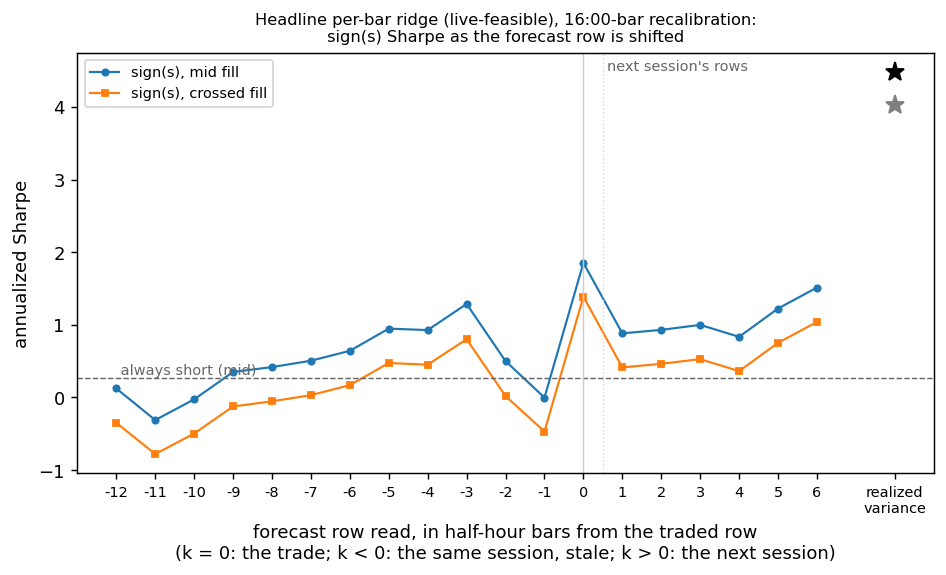
\includegraphics[width=\textwidth]{../results/close_shift_test/shift_test_headline.png}
\caption{The headline forecast's $\mathrm{sign}(s)$ Sharpe as the forecast row is
shifted, on the same \shiftNDays{} days (source:
\texttt{results/close\_shift\_test/shift\_test\_headline.csv}).}
\label{fig:app_shift_test_headline}
\end{figure}
 % 2026-09-29: the shift (dating) test re-run for the headline (close_shift_test_headline.py)
% ============================================================================
% 2026-09-29: the Murphy / threshold analysis and the sample splits parked from
% Section 5.4 (Section~\ref{sec:app_run_parked}: the paper's eight forecasts under
% the session-bar recalibration), re-run for the HEADLINE forecast under the
% 16:00-bar recalibration of Table~\ref{tab:close_option_rules}.  Every number
% below is a macro from generated/appendix_close_murphy_splits.tex, written by
% experiments/close_murphy_splits_headline.py from results/close_murphy_splits/*.csv;
% nothing is typed by hand.  The two recalibrations are never set side by side.
% Input from main.tex after sections/appendix_close_shift_test, so this continues
% Appendix D.
% ============================================================================
% AUTO-GENERATED by experiments/close_murphy_splits_headline.py from results/close_murphy_splits/*.csv -- do not edit.
\begingroup\scriptsize\setlength{\tabcolsep}{2pt}
\begin{longtable}{p{0.27\textwidth}rrrrrrr}
\caption{The comparison set scored two ways on the 866 deck days under the 16:00-bar recalibration: QLIKE against the scorer's target, the elementary score at the trade's threshold (the 15:30 implied variance), the economic loss $|R|\,\mathbf 1\{q\neq\mathrm{sign}(R)\}$, the share of days the forecast falls on the same side of the threshold as the realized variance (same side as $RV$) and the share on which the position has the sign of the settlement return (same side as $R$), and the $\mathrm{sign}(s)$ Sharpe at both fills. The last two rows are rules told the realized variance, and the payoff's sign, in advance.}\label{tab:app_murphy_headline}\\
\toprule
forecast & QLIKE & ES($c{=}1$) & EL & side of $RV$ \% & side of $R$ \% & Sharpe mid & Sharpe crossed \\
\midrule
\endfirsthead
\caption[]{(continued)}\\
\toprule
forecast & QLIKE & ES($c{=}1$) & EL & side of $RV$ \% & side of $R$ \% & Sharpe mid & Sharpe crossed \\
\midrule
\endhead
\bottomrule
\endlastfoot
\textbf{per-bar ridge [live\_feasible]} & 0.101 & 0.100 & 0.349 & 67.4 & 54.7 & 1.90 & 1.44 \\
block-diagonal ridge & 0.106 & 0.100 & 0.380 & 67.2 & 55.0 & 1.00 & 0.53 \\
baseline (HAR + calendar OLS) & 0.117 & 0.099 & 0.374 & 69.7 & 56.6 & 1.17 & 0.69 \\
per-bar lasso [live\_feasible] & 0.096 & 0.096 & 0.351 & 67.8 & 55.1 & 1.83 & 1.36 \\
per-bar ridge [all\_features] & 0.100 & 0.095 & 0.357 & 68.5 & 54.8 & 1.66 & 1.20 \\
per-bar LightGBM [live\_feasible] & 0.098 & 0.105 & 0.356 & 66.2 & 54.6 & 1.69 & 1.22 \\
tuned per-bar LightGBM [all\_features], MSE-selected & 0.101 & 0.107 & 0.352 & 66.4 & 54.6 & 1.81 & 1.35 \\
LSTM live feasible & 0.125 & 0.110 & 0.380 & 63.3 & 53.1 & 1.01 & 0.54 \\
oracle: told RV (sign(RV - slice)) & -- & -- & 0.262 & 100.0 & 62.8 & 4.52 & 4.06 \\
oracle: told the payoff's sign & -- & -- & 0.000 & 62.8 & 100.0 & 17.35 & 17.28 \\
\end{longtable}
\endgroup

\begingroup\scriptsize\setlength{\tabcolsep}{1pt}
\begin{longtable}{llrrrlr}
\caption{Sample splits of the headline's $\mathrm{sign}(s)$ return (midpoint fill) under the 16:00-bar recalibration, beside the paper's block-diagonal ridge scored the same way and always short. $t=\sqrt{n}\,\bar x/s_x$; the Sharpe ratio is annualized with its day-block bootstrap 95\,\% interval (circular blocks of 21 days, 2000 draws); the P\&L share is the split's sum of daily returns over the full-sample sum.}\label{tab:app_splits_headline}\\
\toprule
series & split & $n$ & mean & $t$ & Sharpe [95\,\%] & P\&L share \% \\
\midrule
\endfirsthead
\caption[]{(continued)}\\
\toprule
series & split & $n$ & mean & $t$ & Sharpe [95\,\%] & P\&L share \% \\
\midrule
\endhead
\bottomrule
\endlastfoot
headline sign(s) & all days & 866 & +0.134 & +3.53 & 1.90 [+0.89, +2.94] & 100 \\
headline sign(s) & through 2020-03-31 (the COVID quarter) & 39 & +0.174 & +0.73 & 1.85 [-0.10, +4.02] & 6 \\
headline sign(s) & after 2020-03-31 & 827 & +0.132 & +3.46 & 1.91 [+0.86, +2.99] & 94 \\
headline sign(s) & before 2022-05-16 & 377 & +0.122 & +2.04 & 1.67 [+0.23, +2.90] & 39 \\
headline sign(s) & from 2022-05-16 (daily SPXW listings) & 489 & +0.144 & +2.92 & 2.09 [+0.62, +3.67] & 61 \\
headline sign(s) & settlement pins (R = -1) & 193 & +0.254 & +3.64 & 4.16 [+1.57, +7.33] & 42 \\
headline sign(s) & off pins & 673 & +0.100 & +2.24 & 1.37 [-0.08, +2.71] & 58 \\
reference sign(s) (this scorer) & all days & 866 & +0.071 & +1.86 & 1.00 [-0.03, +2.03] & 100 \\
reference sign(s) (this scorer) & through 2020-03-31 (the COVID quarter) & 39 & -0.116 & -0.48 & -1.22 [-4.86, +0.78] & -7 \\
reference sign(s) (this scorer) & after 2020-03-31 & 827 & +0.080 & +2.08 & 1.15 [+0.10, +2.18] & 107 \\
reference sign(s) (this scorer) & before 2022-05-16 & 377 & +0.063 & +1.05 & 0.86 [-0.80, +2.45] & 38 \\
reference sign(s) (this scorer) & from 2022-05-16 (daily SPXW listings) & 489 & +0.077 & +1.56 & 1.12 [-0.11, +2.44] & 62 \\
reference sign(s) (this scorer) & settlement pins (R = -1) & 193 & +0.285 & +4.12 & 4.71 [+1.23, +8.47] & 89 \\
reference sign(s) (this scorer) & off pins & 673 & +0.010 & +0.22 & 0.13 [-1.20, +1.29] & 11 \\
always short & all days & 866 & +0.014 & +0.38 & 0.20 [-0.62, +1.16] & 100 \\
always short & through 2020-03-31 (the COVID quarter) & 39 & -0.302 & -1.28 & -3.25 [-6.76, +0.59] & -94 \\
always short & after 2020-03-31 & 827 & +0.029 & +0.76 & 0.42 [-0.34, +1.41] & 194 \\
always short & before 2022-05-16 & 377 & -0.033 & -0.55 & -0.45 [-1.52, +0.84] & -98 \\
always short & from 2022-05-16 (daily SPXW listings) & 489 & +0.051 & +1.02 & 0.73 [-0.35, +1.93] & 198 \\
always short & settlement pins (R = -1) & 193 & +1.000 & -- & --  & 1540 \\
always short & off pins & 673 & -0.268 & -6.15 & -3.77 [-4.64, -2.85] & -1440 \\
\end{longtable}
\endgroup

\newcommand{\hmurHQLIKE}{0.101}
\newcommand{\hmurHES}{0.100}
\newcommand{\hmurHQLIKERankSet}{4}
\newcommand{\hmurHESRankSet}{4}
\newcommand{\hmurHQLIKERankAll}{63}
\newcommand{\hmurHESRankAll}{41}
\newcommand{\hmurHSharpeRankAll}{4}
\newcommand{\hmurNAll}{115}
\newcommand{\hmurNSet}{8}
\newcommand{\hmurHHitVar}{67}
\newcommand{\hmurHHitPay}{55}
\newcommand{\hmurHTop}{14}
\newcommand{\hmurOracleAgree}{63}
\newcommand{\hmurOracleMiss}{37}
\newcommand{\hmurOracleShMid}{4.52}
\newcommand{\hmurOracleShX}{4.06}
\newcommand{\hmurPayoffOracleShX}{17.28}
\newcommand{\hmurLeaderAtOne}{per-bar ridge [all\_features]}
\newcommand{\hmurHRankAtOne}{4}
\newcommand{\hmurNGrid}{33}
\newcommand{\hmurNLeadH}{13}
\newcommand{\hmurNLeadLin}{25}
\newcommand{\hmurGridMin}{0.25}
\newcommand{\hmurGridMax}{4}
\newcommand{\hmurRhoQSet}{+0.67}
\newcommand{\hmurRhoQSetLo}{+0.07}
\newcommand{\hmurRhoQSetHi}{+0.90}
\newcommand{\hmurRhoESSet}{+0.24}
\newcommand{\hmurRhoESSetLo}{-0.52}
\newcommand{\hmurRhoESSetHi}{+0.76}
\newcommand{\hmurRhoQAll}{+0.65}
\newcommand{\hmurRhoQAllLo}{+0.13}
\newcommand{\hmurRhoQAllHi}{+0.74}
\newcommand{\hmurRhoESAll}{+0.58}
\newcommand{\hmurRhoESAllLo}{+0.15}
\newcommand{\hmurRhoESAllHi}{+0.77}
\newcommand{\hsplHAllSh}{1.90}
\newcommand{\hsplHAllT}{3.53}
\newcommand{\hsplNCovid}{39}
\newcommand{\hsplHPostCovidN}{827}
\newcommand{\hsplHPostCovidSh}{1.91}
\newcommand{\hsplHPostCovidT}{3.46}
\newcommand{\hsplHPostCovidLo}{0.86}
\newcommand{\hsplHPostCovidHi}{2.99}
\newcommand{\hsplHPreN}{377}
\newcommand{\hsplHPreSh}{1.67}
\newcommand{\hsplHPreT}{2.04}
\newcommand{\hsplHPreLo}{0.23}
\newcommand{\hsplHPreHi}{2.90}
\newcommand{\hsplHPostN}{489}
\newcommand{\hsplHPostSh}{2.09}
\newcommand{\hsplHPostT}{2.92}
\newcommand{\hsplHPostLo}{0.62}
\newcommand{\hsplHPostHi}{3.67}
\newcommand{\hsplRPreSh}{0.86}
\newcommand{\hsplRPostSh}{1.12}
\newcommand{\hsplNPin}{193}
\newcommand{\hsplPinPct}{22.3}
\newcommand{\hsplHPinMean}{+0.25}
\newcommand{\hsplHOffPinMean}{+0.10}
\newcommand{\hsplHPinShare}{42}
\newcommand{\hsplASOffPinMean}{-0.27}
\newcommand{\hsplASPinMean}{+1.00}
\newcommand{\hsplSignBuyMean}{+0.15}
\newcommand{\hsplSignSellMean}{-0.12}
\newcommand{\hsplSignDiff}{0.27}
\newcommand{\hsplSignT}{3.28}
\newcommand{\hsplSignNBuy}{348}
\newcommand{\hsplSignNSell}{518}

\subsection{The Headline Forecast Scored at the Trade's Threshold, and Its Sample Splits}
\label{sec:app_murphy_splits_headline}

\paragraph{The score at the threshold.} Section~\ref{sec:app_run_parked} takes QLIKE
apart by threshold (Equations~\eqref{eq:elementary_score}--\eqref{eq:score_at_threshold})
and reads the trade at the one threshold it uses, the day's implied variance of the last
half hour. Table~\ref{tab:app_murphy_headline} repeats that scoring under the 16:00-bar
recalibration for a comparison set of \hmurNSet{} forecasts --- the headline, the paper's
block-diagonal ridge scored the same way, the HAR $+$ calendar least squares, the
headline's lasso twin, the all-features ridge, an untuned and a tuned tree, and the
LSTM --- and \texttt{scores\_by\_forecast.csv} carries all \hmurNAll{} forecasts of the
master table. QLIKE is against the scorer's target; the identity between QLIKE and the
$\theta^{-2}$ mixture of elementary scores is checked day by day for the headline, and
the identity $\overline{qR}=\overline{|R|}-2\,\overline{EL}$ for every forecast. The
headline scores \hmurHQLIKE{} on QLIKE and \hmurHES{} at the threshold, ranking
\hmurHQLIKERankSet{} and \hmurHESRankSet{} of \hmurNSet{} in the set (\hmurHQLIKERankAll{}
and \hmurHESRankAll{} of \hmurNAll{} overall; its crossed-spread Sharpe ratio ranks
\hmurHSharpeRankAll{} of \hmurNAll{}). It falls on the realized variance's side of the
threshold on \hmurHHitVar{}\,\% of days and on the payoff's side on \hmurHHitPay{}\,\%,
and it is long on \hmurHTop{} of the 20 best long-straddle days.

\paragraph{The Murphy diagram.} Figure~\ref{fig:app_murphy_headline} plots the mean
elementary score against the threshold, in units of the implied variance, from
\hmurGridMin{} to \hmurGridMax{} on a logarithmic grid of \hmurNGrid{} points. The headline
has the lowest score of the set at \hmurNLeadH{} of the \hmurNGrid{} thresholds and a
linear forecast at \hmurNLeadLin{}; at the trade's threshold the leader is
\hmurLeaderAtOne{} and the headline ranks \hmurHRankAtOne{} of \hmurNSet{}.

\paragraph{What a variance forecast can reach.} A rule told the realized variance in
advance takes the payoff's side on \hmurOracleAgree{}\,\% of days (Sharpe
\hmurOracleShMid{} at the midpoint, \hmurOracleShX{} across the spread), against
\hmurPayoffOracleShX{} across the spread for a rule told the payoff's sign; on
\hmurOracleMiss{}\,\% of days the trade's sign is beyond any variance forecast.

\paragraph{Which score orders the forecasts on the trade.} Across the comparison set
the rank correlation of minus the loss with the crossed-spread Sharpe ratio is
\hmurRhoQSet{} for QLIKE (day-block bootstrap 95\,\% interval \hmurRhoQSetLo{} to
\hmurRhoQSetHi{}) and \hmurRhoESSet{} for the score at the threshold (\hmurRhoESSetLo{} to
\hmurRhoESSetHi{}); across all \hmurNAll{} forecasts of the master table it is
\hmurRhoQAll{} (\hmurRhoQAllLo{} to \hmurRhoQAllHi{}) and \hmurRhoESAll{} (\hmurRhoESAllLo{}
to \hmurRhoESAllHi{}). The economic loss is affine in the midpoint P\&L and correlates
perfectly by construction; it is reported as the ceiling.

\paragraph{Sample splits.} Table~\ref{tab:app_splits_headline} repeats the splits of
Section~\ref{sec:app_run_parked} for the headline's $\mathrm{sign}(s)$ return, beside
the paper's forecast scored the same way and always short. Over all 866 days the
headline's annualized Sharpe ratio is \hsplHAllSh{} ($t=\hsplHAllT$). Dropping the
\hsplNCovid{} expiration days through 31~March~2020 leaves \hsplHPostCovidSh{}
($t=\hsplHPostCovidT$, interval \hsplHPostCovidLo{} to \hsplHPostCovidHi{}) on the
remaining \hsplHPostCovidN{} days. Split at 16~May~2022, when SPXW listings became
daily, it is \hsplHPreSh{} ($t=\hsplHPreT$, \hsplHPreLo{} to \hsplHPreHi{}) on the
\hsplHPreN{} days before and \hsplHPostSh{} ($t=\hsplHPostT$, \hsplHPostLo{} to
\hsplHPostHi{}) on the \hsplHPostN{} days after; the paper's forecast scored the same way
reads \hsplRPreSh{} and \hsplRPostSh{}. The straddle expires worthless on \hsplNPin{} of
the days (\hsplPinPct{}\,\%): always short collects \hsplASPinMean{} on them against
\hsplASOffPinMean{} elsewhere, and the headline averages \hsplHPinMean{} on them against
\hsplHOffPinMean{} off them, so pin days supply \hsplHPinShare{}\,\% of its total return.
Read as a same-day sign split, the settlement return averages \hsplSignBuyMean{} on the
\hsplSignNBuy{} days the headline buys and \hsplSignSellMean{} on the \hsplSignNSell{}
days it sells (difference \hsplSignDiff{}, heteroskedasticity-robust $t=\hsplSignT$).

\begin{figure}[H]
\centering
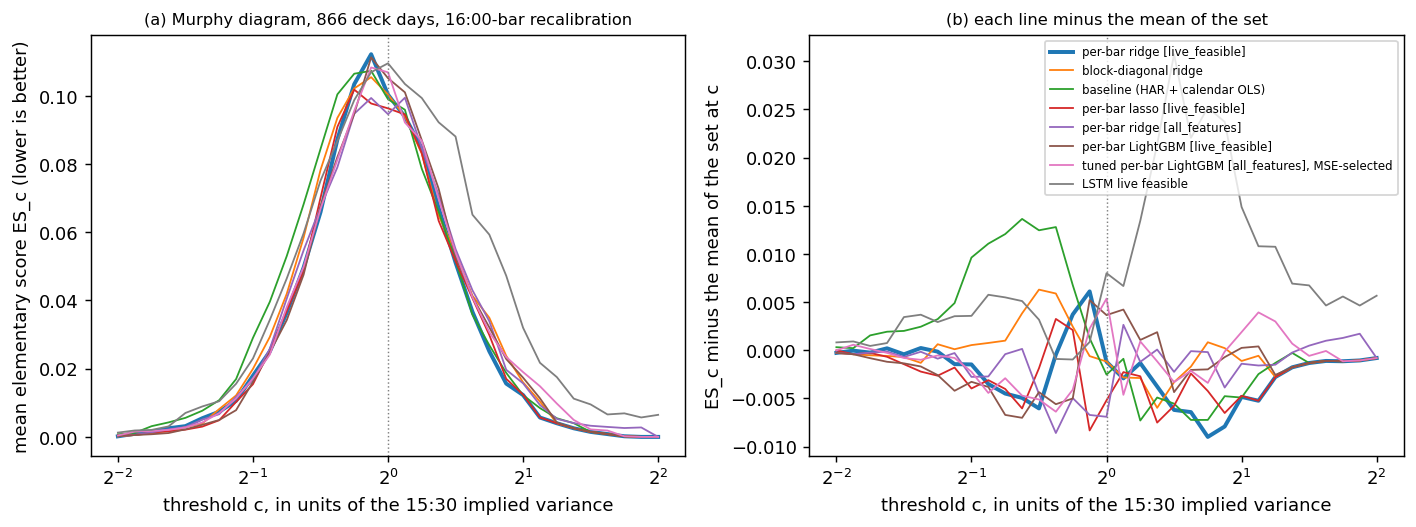
\includegraphics[width=\textwidth]{../results/close_murphy_splits/murphy_headline.png}
\caption{Murphy diagram of the comparison set on the 866 deck days under the 16:00-bar
recalibration. The horizontal axis is the threshold in units of the day's implied
variance of the last half hour, on a logarithmic scale from \hmurGridMin{} to
\hmurGridMax{}; the dotted line at 1 is the threshold the $\mathrm{sign}(s)$ rule uses.
(a) The mean elementary score (lower is better); QLIKE is the area under each line
weighted by $c^{-2}$. (b) Each line minus the mean of the set at the same threshold
(source: \texttt{results/close\_murphy\_splits/murphy\_grid.csv}).}
\label{fig:app_murphy_headline}
\end{figure}
 % 2026-09-29: Murphy/threshold scoring + sample splits re-run for the headline (close_murphy_splits_headline.py)
% ============================================================================
% 2026-09-29: the compounding exercise parked from Section 5.4
% (Section~\ref{sec:app_run_parked}: the paper's block-diagonal ridge under the
% session-bar recalibration), re-run for the HEADLINE forecast under the
% 16:00-bar recalibration of Table~\ref{tab:close_option_rules}.  Every number
% below is a macro from generated/appendix_close_compounding.tex, written by
% experiments/close_compounding_headline.py from results/close_compounding/*.csv;
% nothing is typed by hand.  The two recalibrations are never set side by side.
% Input from main.tex after sections/appendix_close_murphy_splits, so this
% continues Appendix D.
% ============================================================================
% AUTO-GENERATED by experiments/close_compounding_headline.py from results/close_compounding/*.csv -- do not edit.
\begingroup\footnotesize\setlength{\tabcolsep}{3pt}
\begin{longtable}{llrrrrr}
\caption{Compounding at a fixed $f=0.03$ of wealth per day under the 16:00-bar recalibration, 866 days: terminal wealth $W_T=\prod_t(1+f\,q_tR_t)$, annualized log-growth $g$, the largest fall of wealth from its running peak, the worst single-day wealth factor $1+f\min_t R'_t$, and the ruin bound $1/|\min_t R'_t|$ (the sample's worst day). The headline, the paper's block-diagonal ridge scored the same way, and always short, at both fills.}\label{tab:app_compounding_headline}\\
\toprule
series & fill & $W_T$ & $g$ & max DD & worst day & ruin bound \\
\midrule
\endfirsthead
\caption[]{(continued)}\\
\toprule
series & fill & $W_T$ & $g$ & max DD & worst day & ruin bound \\
\midrule
\endhead
\bottomrule
\endlastfoot
headline sign(s) & mid & 20.18 & +0.87 & 34\,\% & 0.837 & 0.18 \\
headline sign(s) & crossed & 8.55 & +0.62 & 38\,\% & 0.832 & 0.18 \\
reference sign(s) (this scorer) & mid & 3.89 & +0.40 & 42\,\% & 0.837 & 0.18 \\
reference sign(s) (this scorer) & crossed & 1.62 & +0.14 & 50\,\% & 0.832 & 0.18 \\
always short & mid & 0.86 & -0.04 & 55\,\% & 0.691 & 0.10 \\
always short & crossed & 0.33 & -0.32 & 74\,\% & 0.671 & 0.09 \\
\end{longtable}
\endgroup

\newcommand{\cmpF}{0.03}
\newcommand{\cmpHW}{20.2}
\newcommand{\cmpHG}{+0.87}
\newcommand{\cmpHDD}{34}
\newcommand{\cmpHWorst}{16}
\newcommand{\cmpHRuin}{0.18}
\newcommand{\cmpHWX}{8.5}
\newcommand{\cmpHGX}{+0.62}
\newcommand{\cmpHDDX}{38}
\newcommand{\cmpRW}{3.9}
\newcommand{\cmpRG}{+0.40}
\newcommand{\cmpRWX}{1.6}
\newcommand{\cmpAW}{0.86}
\newcommand{\cmpAG}{-0.04}
\newcommand{\cmpARuin}{0.10}
\newcommand{\cmpAWX}{0.33}
\newcommand{\cmpNAll}{220}
\newcommand{\cmpNPosMid}{218}
\newcommand{\cmpNPosX}{208}
\newcommand{\cmpWLoMid}{0.6}
\newcommand{\cmpWHiMid}{20.4}
\newcommand{\cmpWLoX}{0.2}
\newcommand{\cmpWHiX}{8.6}
\newcommand{\cmpHRankMid}{2}
\newcommand{\cmpHRankX}{2}
\newcommand{\cmpNYears}{5}
\newcommand{\cmpNPosYears}{4}
\newcommand{\cmpNegYears}{2022 is $-0.01$}
\newcommand{\cmpNPosYearsX}{4}
\newcommand{\cmpNegYearsX}{2022 is $-0.19$}
\newcommand{\cmpYearsMid}{2020: $+0.87$, 2021: $+0.79$, 2022: $-0.01$, 2023: $+1.29$, 2024: $+2.15$}
\newcommand{\cmpYearsX}{2020: $+0.44$, 2021: $+0.48$, 2022: $-0.19$, 2023: $+1.11$, 2024: $+1.96$}

\subsection{The Headline Forecast Compounded at a Fixed Fraction of Wealth}
\label{sec:app_compounding_headline}

\paragraph{What is computed.} The fixed-fraction exercise of
Section~\ref{sec:close_option_methods} --- a share $f=\cmpF$ of current wealth deployed
as straddle premium every day, the same on every day and for every rule, wealth
$W_T=\prod_t(1+f\,q_tR_t)$, the annualized mean of $\log(1+fR'_t)$ as the growth rate,
every wealth factor asserted positive --- repeated for the headline's $\mathrm{sign}(s)$
positions under the 16:00-bar recalibration, on the 866 days and at both fills, beside the
paper's block-diagonal ridge scored the same way and always short
(Table~\ref{tab:app_compounding_headline}, Figure~\ref{fig:app_compounding_headline}).
The midpoint frame is the one Section~\ref{sec:app_run_parked} reports for the paper's
forecast under the other recalibration; the crossed frame pays the ask and hits the bid on
every day.

\paragraph{Reading.} At the midpoint the headline turns one unit of wealth into \cmpHW{}
over the sample (annualized log-growth \cmpHG{}), with a maximum wealth drawdown of
\cmpHDD{} percent and a worst single day that removes \cmpHWorst{} percent of wealth; the
ruin bound $1/|\min_t R'_t|$ is \cmpHRuin{} for the headline and \cmpARuin{} for always
short, so \cmpF{} sits inside both. Across the spread it ends at \cmpHWX{}
(log-growth \cmpHGX{}, drawdown \cmpHDDX{} percent). The paper's forecast scored the same
way ends at \cmpRW{} at the midpoint (\cmpRG{}) and \cmpRWX{} across the spread; always
short ends at \cmpAW{} (\cmpAG{}) and \cmpAWX{}. Of the \cmpNAll{} distinct forecasts of the
master table (the rest-of-day check rows, exact copies of their per-bar twins, left out),
\cmpNPosMid{} compound above one unit at the midpoint (terminal wealth \cmpWLoMid{}
to \cmpWHiMid{}; the headline ranks \cmpHRankMid{}) and \cmpNPosX{} across the spread
(\cmpWLoX{} to \cmpWHiX{}; the headline ranks \cmpHRankX{}). By calendar year, annualized
from the days traded in each, the headline's midpoint log-growth is positive in
\cmpNPosYears{} of \cmpNYears{} years (\cmpYearsMid{}) and across the spread in
\cmpNPosYearsX{} (\cmpYearsX{}).

\begin{figure}[H]
\centering
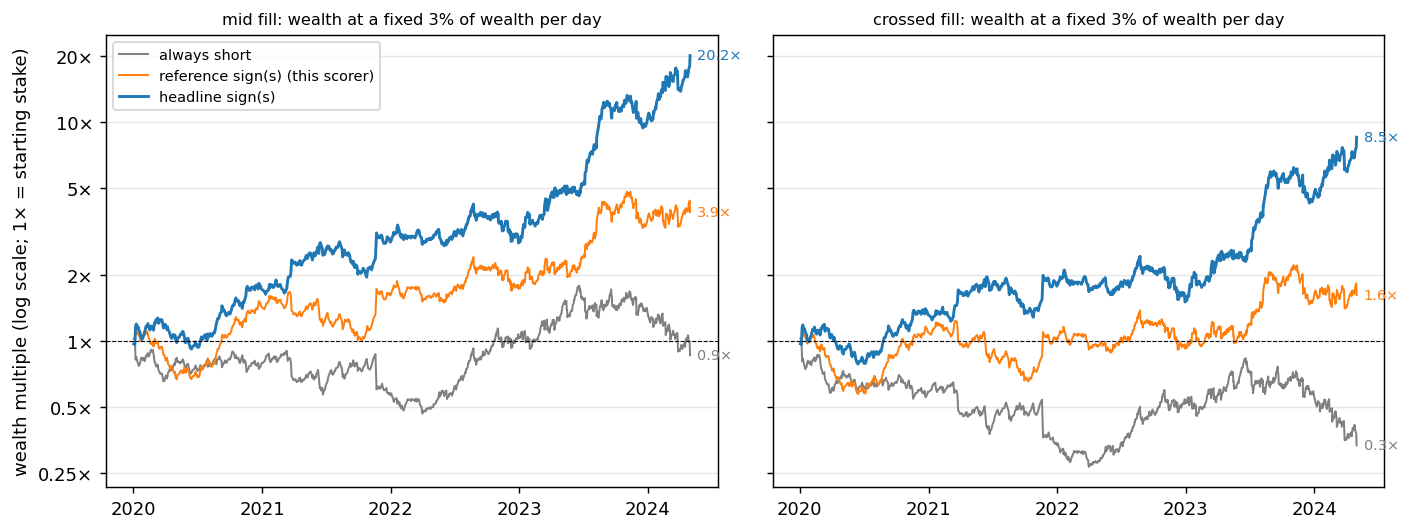
\includegraphics[width=\textwidth]{../results/close_compounding/wealth_headline.png}
\caption{Wealth at a fixed \cmpF{} of wealth per day, 866 days, under the 16:00-bar
recalibration: the headline's $\mathrm{sign}(s)$, the paper's block-diagonal ridge scored the
same way, and always short; midpoint fill (left) and crossed spread (right), log scale
(source: \texttt{results/close\_compounding/fixedfrac\_headline.csv}).}
\label{fig:app_compounding_headline}
\end{figure}
 % 2026-09-29: fixed-fraction compounding re-run for the headline (close_compounding_headline.py)
% ============================================================================
% 2026-09-30 (agent L4): the 16:00 campaign (writeup/CAMPAIGN_16H_2026-09-29.md) as a
% record, one change at a time.  Every number below is a macro from
% generated/appendix_campaign_16h_numbers.tex and every table a file
% generated/appendix_campaign_16h_<table>.tex, both written by
%     python writeup/make_appendix_campaign_16h_tex.py
% from the campaign's CSVs (each table's source is named in a comment above it and
% inside the generated file); nothing is typed by hand.  Wording: sign(s) rule,
% straddle, last-30-min trade; no cluster or lab names in prose (the compute table
% labels them cluster A / B).  Input from main.tex after
% sections/appendix_close_compounding, so this continues Appendix D.
% ============================================================================
% AUTO-GENERATED by writeup/make_appendix_campaign_16h_tex.py -- do not edit.
% Every macro is read from the campaign's CSVs / summaries (sources in the table files and
% in the script); prose in sections/appendix_campaign_16h.tex quotes numbers only through these.
\newcommand{\campPOldBase}{34}
\newcommand{\campPNewBase}{22}
\newcommand{\campKeptLinBase}{17}
\newcommand{\campPOldLive}{244}
\newcommand{\campPNewLive}{232}
\newcommand{\campKeptLinLive}{136--138}
\newcommand{\campPOldAll}{640}
\newcommand{\campPNewAll}{628}
\newcommand{\campKeptLinAll}{360--378}
\newcommand{\campNSessionEdge}{12}
\newcommand{\campNSessionEdgeHalf}{6}
\newcommand{\campNLinear}{76}
\newcommand{\campNLinearMasked}{75}
\newcommand{\campMaskDropAgree}{75}
\newcommand{\campOLSN}{1}
\newcommand{\campOLSMaxRel}{\ensuremath{8\times10^{-15}}}
\newcommand{\campOLSMoved}{0}
\newcommand{\campRidgeN}{25}
\newcommand{\campRidgeMaxRel}{\ensuremath{4\times10^{-10}}}
\newcommand{\campRidgeMoved}{0}
\newcommand{\campLassoN}{25}
\newcommand{\campLassoMaxRel}{\ensuremath{9\times10^{-2}}}
\newcommand{\campLassoMoved}{7}
\newcommand{\campEnetN}{25}
\newcommand{\campEnetMaxRel}{\ensuremath{9\times10^{-2}}}
\newcommand{\campEnetMoved}{10}
\newcommand{\campMovedTol}{\ensuremath{1\times10^{-8}}}
\newcommand{\campPosChanged}{9}
\newcommand{\campTradeDays}{866}
\newcommand{\campMaxDSharpeLin}{0.06}
\newcommand{\campAttrN}{17}
\newcommand{\campAttrRepeat}{17}
\newcommand{\campAttrDesignN}{13}
\newcommand{\campAttrDesignLo}{\ensuremath{5.5\times10^{-4}}}
\newcommand{\campAttrDesignHi}{\ensuremath{1.7\times10^{-2}}}
\newcommand{\campAttrMachineN}{12}
\newcommand{\campAttrMachineLo}{\ensuremath{7.3\times10^{-4}}}
\newcommand{\campAttrMachineHi}{\ensuremath{8.1\times10^{-2}}}
\newcommand{\campLSTMDedupLo}{2.5}
\newcommand{\campLSTMDedupHi}{7.6}
\newcommand{\campRodChecks}{9}
\newcommand{\campRodBeforeMax}{\ensuremath{1.7\times10^{-2}}}
\newcommand{\campRodBeforeSameMin}{865}
\newcommand{\campRodDeck}{866}
\newcommand{\campRodAfterBit}{9}
\newcommand{\campRodRows}{1{,}469}
\newcommand{\campRodArms}{117}
\newcommand{\campRodMaskSame}{117}
\newcommand{\campKeptBase}{17}
\newcommand{\campKeptBaseLo}{17}
\newcommand{\campKeptBaseHi}{17}
\newcommand{\campPBase}{22}
\newcommand{\campKeptLive}{138}
\newcommand{\campKeptLiveLo}{136}
\newcommand{\campKeptLiveHi}{145}
\newcommand{\campPLive}{232}
\newcommand{\campKeptAll}{369}
\newcommand{\campKeptAllLo}{360}
\newcommand{\campKeptAllHi}{378}
\newcommand{\campPAll}{628}
\newcommand{\campKeptRefits}{1{,}469}
\newcommand{\campMaskTreeN}{36}
\newcommand{\campMaskTreeQBelow}{0}
\newcommand{\campMaskTreeQAbove}{5}
\newcommand{\campMaskTreeSBelow}{1}
\newcommand{\campMaskTreeSAbove}{0}
\newcommand{\campMaskMedAbsQ}{0.7}
\newcommand{\campMaskLSTMN}{3}
\newcommand{\campMaskLSTMQBelow}{1}
\newcommand{\campMaskLSTMQAbove}{0}
\newcommand{\campMaskLSTMSBelow}{0}
\newcommand{\campMaskLSTMSAbove}{0}
\newcommand{\campMaskLSTMAllQ}{\ensuremath{-}17.1}
\newcommand{\campMaskLSTMAllQCI}{[\ensuremath{-}33.2, \ensuremath{-}4.2]}
\newcommand{\campTOneTenN}{9}
\newcommand{\campTOneTenQBelow}{3}
\newcommand{\campTOneTenQAbove}{0}
\newcommand{\campTOneTenSBelow}{0}
\newcommand{\campTOneTenSAbove}{1}
\newcommand{\campTOneTenQLo}{\ensuremath{-}3.6}
\newcommand{\campTOneTenQHi}{\ensuremath{-}0.8}
\newcommand{\campRSOneTenN}{9}
\newcommand{\campRSOneTenQBelow}{1}
\newcommand{\campRSOneTenQAbove}{0}
\newcommand{\campRSOneTenSBelow}{0}
\newcommand{\campRSOneTenSAbove}{0}
\newcommand{\campRSOneTenQLo}{\ensuremath{-}2.2}
\newcommand{\campRSOneTenQHi}{\ensuremath{+}0.2}
\newcommand{\campRSVsTN}{9}
\newcommand{\campRSVsTQBelow}{0}
\newcommand{\campRSVsTQAbove}{6}
\newcommand{\campRSVsTSBelow}{0}
\newcommand{\campRSVsTSAbove}{0}
\newcommand{\campRSVsTQLo}{\ensuremath{+}3.6}
\newcommand{\campRSVsTQHi}{\ensuremath{+}17.9}
\newcommand{\campLSTMCadN}{3}
\newcommand{\campLSTMCadQBelow}{2}
\newcommand{\campLSTMCadQAbove}{0}
\newcommand{\campLSTMCadSBelow}{0}
\newcommand{\campLSTMCadSAbove}{0}
\newcommand{\campLSTMCadBase}{\ensuremath{-}1.9}
\newcommand{\campLSTMCadBaseCI}{[\ensuremath{-}3.5, \ensuremath{-}0.3]}
\newcommand{\campLSTMCadLive}{\ensuremath{-}2.5}
\newcommand{\campLSTMCadLiveCI}{[\ensuremath{-}7.8, \ensuremath{+}3.2]}
\newcommand{\campLSTMCadAll}{\ensuremath{-}10.1}
\newcommand{\campLSTMCadAllCI}{[\ensuremath{-}18.0, \ensuremath{-}2.0]}
\newcommand{\campRidgeTreeN}{36}
\newcommand{\campRidgeTreeQBelow}{0}
\newcommand{\campRidgeTreeQAbove}{18}
\newcommand{\campRidgeTreeSBelow}{0}
\newcommand{\campRidgeTreeSAbove}{0}
\newcommand{\campRidgeBestTree}{T1 LightGBM \texttt{live\_feasible}}
\newcommand{\campRidgeBestTreeQ}{\ensuremath{-}5.0}
\newcommand{\campRidgeBestTreeQCI}{[\ensuremath{-}11.5, \ensuremath{+}0.4]}
\newcommand{\campRidgeLSTMN}{3}
\newcommand{\campRidgeLSTMQBelow}{0}
\newcommand{\campRidgeLSTMQAbove}{3}
\newcommand{\campRidgeLSTMSBelow}{0}
\newcommand{\campRidgeLSTMSAbove}{0}
\newcommand{\campRidgeLSTMBase}{\ensuremath{+}6.8}
\newcommand{\campRidgeLSTMLive}{\ensuremath{+}18.6}
\newcommand{\campRidgeLSTMAll}{\ensuremath{+}30.0}
\newcommand{\campOptTrials}{50}
\newcommand{\campOptPoints}{1{,}469}
\newcommand{\campOptExch}{20}
\newcommand{\campOptLateLo}{27}
\newcommand{\campOptLateHi}{40}
\newcommand{\campOptGainTwentyFiveLo}{1.1}
\newcommand{\campOptGainTwentyFiveHi}{2.1}
\newcommand{\campOptGainTwentyFiveMedLo}{0.4}
\newcommand{\campOptGainTwentyFiveMedHi}{1.2}
\newcommand{\campOptGainFortyLo}{0.3}
\newcommand{\campOptGainFortyHi}{0.7}
\newcommand{\campOptGainFortyMedMax}{0.0}
\newcommand{\campOptPickDiffLo}{61}
\newcommand{\campOptPickDiffHi}{74}
\newcommand{\campOptShippedHi}{1.1}
\newcommand{\campBudN}{54}
\newcommand{\campBudQBelow}{0}
\newcommand{\campBudQAbove}{1}
\newcommand{\campBudSBelow}{1}
\newcommand{\campBudSAbove}{0}
\newcommand{\campTPN}{27}
\newcommand{\campTPQBelow}{8}
\newcommand{\campTPQAbove}{0}
\newcommand{\campTPSBelow}{0}
\newcommand{\campTPSAbove}{0}
\newcommand{\campTPBelowWho}{LightGBM \texttt{baseline} (TUNE\_PER 5, 25); random forest \texttt{live\_feasible} (TUNE\_PER 1, 5, 25); random forest \texttt{all\_features} (TUNE\_PER 1, 5, 25)}
\newcommand{\campTPRuleN}{9}
\newcommand{\campTPRuleQBelow}{2}
\newcommand{\campTPRuleQAbove}{0}
\newcommand{\campTPRuleSBelow}{1}
\newcommand{\campTPRuleSAbove}{0}
\newcommand{\campOptTN}{36}
\newcommand{\campOptTQBelow}{0}
\newcommand{\campOptTQAbove}{19}
\newcommand{\campOptTSBelow}{0}
\newcommand{\campOptTSAbove}{0}
\newcommand{\campOptRSN}{36}
\newcommand{\campOptRSQBelow}{8}
\newcommand{\campOptRSQAbove}{3}
\newcommand{\campOptRSSBelow}{1}
\newcommand{\campOptRSSAbove}{0}
\newcommand{\campOptRidgeN}{36}
\newcommand{\campOptRidgeQBelow}{0}
\newcommand{\campOptRidgeQAbove}{14}
\newcommand{\campOptRidgeSBelow}{2}
\newcommand{\campOptRidgeSAbove}{0}
\newcommand{\campOptRSBelowWho}{XGBoost \texttt{live\_feasible} (TUNE\_PER 250); XGBoost \texttt{all\_features} (TUNE\_PER 250); random forest \texttt{live\_feasible} (TUNE\_PER 1, 5, 25); random forest \texttt{all\_features} (TUNE\_PER 1, 5, 25)}
\newcommand{\campPickLgbmMcsLo}{14}
\newcommand{\campPickLgbmMcsHi}{23}
\newcommand{\campPickRfDepthLo}{20}
\newcommand{\campPickRfDepthHi}{28}
\newcommand{\campPickRfDepthPrior}{17}
\newcommand{\campPickLambdaHighMax}{0.0}
\newcommand{\campPickLambdaPriorLo}{5.1}
\newcommand{\campLstmiVsLSTMN}{3}
\newcommand{\campLstmiVsLSTMQBelow}{1}
\newcommand{\campLstmiVsLSTMQAbove}{0}
\newcommand{\campLstmiVsLSTMSBelow}{0}
\newcommand{\campLstmiVsLSTMSAbove}{0}
\newcommand{\campLstmiVsRidgeN}{3}
\newcommand{\campLstmiVsRidgeQBelow}{0}
\newcommand{\campLstmiVsRidgeQAbove}{3}
\newcommand{\campLstmiVsRidgeSBelow}{0}
\newcommand{\campLstmiVsRidgeSAbove}{0}
\newcommand{\campLstmiStepBase}{19}
\newcommand{\campLstmiKeptBase}{19}
\newcommand{\campLstmiKeptBaseLo}{16}
\newcommand{\campLstmiKeptBaseHi}{19}
\newcommand{\campLstmiStepLive}{54}
\newcommand{\campLstmiKeptLive}{40}
\newcommand{\campLstmiKeptLiveLo}{37}
\newcommand{\campLstmiKeptLiveHi}{41}
\newcommand{\campLstmiStepAll}{120}
\newcommand{\campLstmiKeptAll}{80}
\newcommand{\campLstmiKeptAllLo}{74}
\newcommand{\campLstmiKeptAllHi}{82}
\newcommand{\campLstmiTunings}{18}
\newcommand{\campLstmiNThirteen}{3}
\newcommand{\campLstmiNFortyEight}{9}
\newcommand{\campLstmiNNinetySix}{6}
\newcommand{\campLstmiRefits}{1{,}469}
\newcommand{\campXColsLive}{28}
\newcommand{\campXColsAll}{94}
\newcommand{\campXMaxAbs}{\ensuremath{2.6\times10^{-11}}}
\newcommand{\campXHosts}{12}
\newcommand{\campXSamePairs}{18}
\newcommand{\campSameClassTrials}{900/900}
\newcommand{\campSameClassTrialsRep}{900/900}
\newcommand{\campSameClassFcst}{1{,}620/1{,}620}
\newcommand{\campXTrialsLgbm}{100/300}
\newcommand{\campXFcstLgbm}{5/360}
\newcommand{\campXFcstMaxLgbm}{0.103}
\newcommand{\campXPicksLgbm}{not identical}
\newcommand{\campXTrialsXgb}{211/300}
\newcommand{\campXFcstXgb}{344/360}
\newcommand{\campXFcstMaxXgb}{0.033}
\newcommand{\campXPicksXgb}{identical}
\newcommand{\campXTrialsRf}{283/300}
\newcommand{\campXFcstRf}{360/360}
\newcommand{\campXFcstMaxRf}{0.000}
\newcommand{\campXPicksRf}{identical}
\newcommand{\campXcPoints}{20}
\newcommand{\campXcPickLgbm}{18}
\newcommand{\campXcPickXgb}{0}
\newcommand{\campXcPickRf}{0}
\newcommand{\campXcValLgbm}{3.6}
\newcommand{\campXcValXgb}{\ensuremath{3.9\times10^{-3}}}
\newcommand{\campXcFcstXgb}{\ensuremath{7.3\times10^{-3}}}
\newcommand{\campXcSame}{20}
\newcommand{\campClassRelTen}{4.5}
\newcommand{\campClassQTen}{\ensuremath{-}0.1}
\newcommand{\campClassQTenCI}{[\ensuremath{-}0.8, \ensuremath{+}0.5]}
\newcommand{\campClassSTen}{\ensuremath{-}0.26}
\newcommand{\campClassSTenCI}{[\ensuremath{-}0.68, \ensuremath{+}0.11]}
\newcommand{\campClassRelOne}{5.5}
\newcommand{\campClassQOne}{\ensuremath{-}0.1}
\newcommand{\campClassQOneCI}{[\ensuremath{-}0.8, \ensuremath{+}0.8]}
\newcommand{\campClassSOne}{\ensuremath{+}0.07}
\newcommand{\campClassSOneCI}{[\ensuremath{-}0.30, \ensuremath{+}0.42]}
\newcommand{\campClassRows}{1{,}469}
\newcommand{\campLstmiXTune}{17/18}
\newcommand{\campLstmiXChunk}{19/20}
\newcommand{\campSMDiffer}{35}
\newcommand{\campSMMaxLgbm}{0.65}
\newcommand{\campSMMaxXgb}{0.17}
\newcommand{\campSMMaxRf}{0.0025}
\newcommand{\campSMN}{81}
\newcommand{\campSMQBelow}{2}
\newcommand{\campSMQAbove}{3}
\newcommand{\campSMSBelow}{0}
\newcommand{\campSMSAbove}{0}
\newcommand{\campSMSharpeExcl}{0}
\newcommand{\campCChunks}{214}
\newcommand{\campCChunkClasses}{1}
\newcommand{\campHChunks}{327}
\newcommand{\campHChunkClasses}{1}
\newcommand{\campHGateChunks}{6}
\newcommand{\campMTKeysBoth}{136}
\newcommand{\campMTKeysNew}{114}
\newcommand{\campMTHeadQ}{0.1005}
\newcommand{\campMTHeadQBefore}{0.1005}
\newcommand{\campMTHeadPos}{0}
\newcommand{\campMTHeadDays}{866}
\newcommand{\campMTHeadS}{1.90}
\newcommand{\campMTHeadSX}{1.44}
\newcommand{\campMTHeadMaxRel}{\ensuremath{1.0\times10^{-12}}}
\newcommand{\campMTSigWho}{per-bar XGBoost [live\_feasible]: 1.70 $\to$ 1.27, \ensuremath{-}0.43 [\ensuremath{-}0.94, \ensuremath{-}0.03]; per-bar XGBoost [baseline]: 1.12 $\to$ 0.92, \ensuremath{-}0.21 [\ensuremath{-}0.42, \ensuremath{-}0.04]; per-bar LSTM [baseline]: 0.61 $\to$ 1.26, \ensuremath{+}0.65 [\ensuremath{+}0.05, \ensuremath{+}1.27]}
\newcommand{\campMTSigN}{3}
\newcommand{\campMTNOther}{219}
\newcommand{\campMTBeatMid}{0}
\newcommand{\campMTBeatCrossed}{0}
\newcommand{\campMTWorseMid}{43}
\newcommand{\campMTQBetter}{3}
\newcommand{\campMTQWorse}{37}
\newcommand{\campMTQBetterFamily}{HAR-ladder variants}
\newcommand{\campMTQBetterWho}{per-bar elastic net [live\_feasible], HAR ladder base3: QLIKE 0.0934 (\ensuremath{-}7.1\,\%, interval on the daily difference [\ensuremath{-}0.0144, \ensuremath{-}0.0019]), $\Delta$Sharpe mid \ensuremath{-}0.33 [\ensuremath{-}0.91, \ensuremath{+}0.34]; per-bar elastic net [live\_feasible], HAR ladder base2: QLIKE 0.0944 (\ensuremath{-}6.1\,\%, interval on the daily difference [\ensuremath{-}0.0122, \ensuremath{-}0.0012]), $\Delta$Sharpe mid \ensuremath{-}0.15 [\ensuremath{-}0.82, \ensuremath{+}0.59]; per-bar lasso [live\_feasible], HAR ladder base2: QLIKE 0.0948 (\ensuremath{-}5.8\,\%, interval on the daily difference [\ensuremath{-}0.0126, \ensuremath{-}0.0001]), $\Delta$Sharpe mid \ensuremath{-}0.12 [\ensuremath{-}0.76, \ensuremath{+}0.55]}
\newcommand{\campFIRidgeNoise}{1.7}
\newcommand{\campFILeadN}{54}
\newcommand{\campFILead}{52}
\newcommand{\campFISpearmanTrees}{0.90}
\newcommand{\campFISpearmanTreesMin}{0.66}
\newcommand{\campDvsClaims}{23}
\newcommand{\campDvsClaimsSame}{20}
\newcommand{\campDvsLgbmQLive}{\ensuremath{+}0.0004}
\newcommand{\campDvsLgbmQLiveCI}{[\ensuremath{-}0.0012, \ensuremath{+}0.0020]}
\newcommand{\campDvsLgbmSLive}{\ensuremath{+}0.04}
\newcommand{\campDvsLgbmSLiveCI}{[\ensuremath{-}0.30, \ensuremath{+}0.39]}
\newcommand{\campDvsLgbmQAll}{\ensuremath{+}0.0002}
\newcommand{\campDvsLgbmQAllCI}{[\ensuremath{-}0.0012, \ensuremath{+}0.0016]}
\newcommand{\campDvsLgbmSAll}{\ensuremath{+}0.20}
\newcommand{\campDvsLgbmSAllCI}{[\ensuremath{-}0.27, \ensuremath{+}0.77]}
\newcommand{\campDvsLinMaxRel}{\ensuremath{3.3\times10^{-12}}}
\newcommand{\campDvsRfLive}{13.2 $\to$ 6.8}
\newcommand{\campComputeOptunaAlloc}{1422.6}
\newcommand{\campComputeOptunaPeak}{900}


% Shrink a table to the text width only when it is wider; never enlarge it.
\newsavebox{\campbox}
\newcommand{\campfit}[1]{%
  \sbox{\campbox}{#1}%
  \ifdim\wd\campbox>\textwidth
    \resizebox{\textwidth}{!}{\usebox{\campbox}}%
  \else
    \usebox{\campbox}%
  \fi}

\subsection{The 16:00 Models Re-run: Design, Mask, Cadence, Tuning}
\label{sec:app_campaign_16h}

Every per-bar model that forecasts the 16:00 bar (the 15:30--16:00 half hour, issued at
15:30, the bar the last-30-min trade is decided on) was re-run with one change at a time:
the design (\ref{sec:app_camp_design}), a per-window column mask for the trees and the LSTM
(\ref{sec:app_camp_mask}), the refit cadence (\ref{sec:app_camp_cadence}), the tuning
(\ref{sec:app_camp_tuning}); an intraday-sequence LSTM was added
(\ref{sec:app_camp_lstmi}). The section also records what the re-run showed about
reproducibility across CPUs (\ref{sec:app_camp_repro}), the master table before and after
(\ref{sec:app_camp_master}), the importance and density studies on the new design
(\ref{sec:app_camp_featimp}) and the compute used (\ref{sec:app_camp_compute}). Nothing is
discarded: a rung that did worse is reported beside one that did better.

Every comparison uses the research scorer (the 16:00 bar recalibrated on its own), the same
\campTradeDays{} trade days, and the $\mathrm{sign}(s)$ rule on the straddle (nearest
out-of-the-money call and put, same-day expiry, one position). A difference is $a-b$; a
QLIKE difference is given in percent of $b$'s QLIKE, with its 95\,\% paired day-block
bootstrap interval in the same units (negative = $a$ has the lower loss); a Sharpe
difference is the midpoint-fill $\mathrm{sign}(s)$ Sharpe ratio of $a$ minus that of $b$,
with its interval. In the grid tables each cell holds the QLIKE difference on its first line
and the Sharpe difference on its second. Input sets: \texttt{baseline} (the HAR ladder and
the calendar columns), \texttt{live\_feasible} (the inputs a 15:30 forecaster can rebuild
live) and \texttt{all\_features}. Key to the design columns named below:
\texttt{har\_ma\_*} is the bar's realized variance averaged over the last 1, 5, 25, 125,
625 and 3125 bars (the HAR ladder, \texttt{har\_ma\_k} one rung);
\texttt{har\_ma\_k\_x\_open} and \texttt{har\_ma\_k\_x\_close} are that rung times the
session-open and session-close indicators (the session-edge interactions).

% ----------------------------------------------------------------------------
\subsubsection{The design: the session-edge columns}
\label{sec:app_camp_design}

The session-edge interactions were built for the pooled 48-bar models. In a
one-bar-per-session series at the 16:00 bar the \campNSessionEdgeHalf{}
\texttt{har\_ma\_k\_x\_open} columns are identically zero and the \campNSessionEdgeHalf{}
\texttt{har\_ma\_k\_x\_close} columns are exact copies of \texttt{har\_ma\_k}. The
\campNSessionEdge{} columns were dropped from the per-bar design and kept in the pooled
models: \texttt{baseline} goes from \campPOldBase{} to \campPNewBase{} columns,
\texttt{live\_feasible} from \campPOldLive{} to \campPNewLive{}, \texttt{all\_features} from
\campPOldAll{} to \campPNewAll{} (Table~\ref{tab:app_camp_design}).

The linear arms' identifiability mask --- at every penalty tune, drop the columns constant
on the tuning window and the exact copies of an earlier kept column --- had already removed
all of them: in \campMaskDropAgree{} of the \campNLinearMasked{} masked linear forecasts the
number of masked columns per tune falls by exactly the number of dropped columns, and the
columns each fit keeps are the same before and after (last column of
Table~\ref{tab:app_camp_design}). The fits solve the same problem, and the \campNLinear{}
linear forecasts of the master table move by rounding only
(Table~\ref{tab:app_camp_linear}): OLS by at most \campOLSMaxRel{} and ridge by at most
\campRidgeMaxRel{} (relative change of the 16:00 forecast). The lasso and the elastic net
move by up to \campLassoMaxRel{} and \campEnetMaxRel{}, on the rows of one penalty-tune
period, in \campLassoMoved{} of \campLassoN{} and \campEnetMoved{} of \campEnetN{} forecasts;
positions change on \campPosChanged{} of the \campNLinear{}\,$\times$\,\campTradeDays{}
forecast-days, and no Sharpe ratio moves by more than \campMaxDSharpeLin{}. A control on the
\campAttrN{} arms that moved attributes this to the solvers' floating-point path: the
pre-change code re-run on the same CPU architecture reproduces its first run bit for bit in
\campAttrRepeat{} of \campAttrN{}; the new code against the pre-change code on one
architecture moves \campAttrDesignN{} of them, by \campAttrDesignLo{} to
\campAttrDesignHi{}; the pre-change code alone, moved to another machine, moves
\campAttrMachineN{}, by \campAttrMachineLo{} to \campAttrMachineHi{}. The LSTM, which had no
mask at that step, moved more (median relative change of the 16:00 forecast
\campLSTMDedupLo--\campLSTMDedupHi\,\% over the three input sets; a new input width also
redraws its initial weights).

The rest-of-day model's \campRodArms{} arms were re-run on the same design; their mask fell
by exactly \campNSessionEdge{} columns per tune in \campRodMaskSame{} of them. The master
table's \campRodChecks{} check rows (the rest-of-day model at 15:30, which should equal its
per-bar 16:00 twin) had differed from their twins by up to \campRodBeforeMax{} (the same
position on as few as \campRodBeforeSameMin{} of \campRodDeck{} days); they are now
bit-identical to their twins in \campRodAfterBit{} of \campRodChecks{}, on every one of the
\campRodRows{} 16:00 rows.

% Source: results/linear_subsection_dedup/change_by_arm.csv
\begin{table}[H]
\centering
\caption{The per-bar design before and after the session-edge columns were dropped, and
the linear arms' identifiability mask per penalty tune (range over tunes) for the per-bar
ridge: the columns it masked fall by exactly the columns removed, so the columns kept are
unchanged.}
\label{tab:app_camp_design}
\campfit{\small% AUTO-GENERATED by writeup/make_appendix_campaign_16h_tex.py -- do not edit.
% Source: results/linear_subsection_dedup/change_by_arm.csv (rows sub_ridge_<input set>)
\begin{tabular}{lrrrrrr}
\toprule
input set & \shortstack{columns\\before} & \shortstack{columns\\after} & removed & \shortstack{masked per\\tune, before} & \shortstack{masked per\\tune, after} & \shortstack{kept per\\tune} \\
\midrule
\texttt{baseline} & 34 & 22 & 12 & 17 & 5 & 17 \\
\texttt{live\_feasible} & 244 & 232 & 12 & 106--108 & 94--96 & 136--138 \\
\texttt{all\_features} & 640 & 628 & 12 & 262--280 & 250--268 & 360--378 \\
\bottomrule
\end{tabular}
}
\end{table}

% Source: results/linear_subsection_dedup/change_by_arm.csv, gates.csv
\begin{table}[H]
\centering
\caption{The master table's per-bar linear forecasts, new design minus old, by estimator:
the largest and the median (over forecasts) of the per-forecast maximum and median relative
change of the 16:00 forecast, the forecasts whose maximum exceeds the reproduction gate's
bound, the trade positions changed (forecast-days, of \campTradeDays{} per forecast) and the
largest change of a $\mathrm{sign}(s)$ Sharpe ratio (midpoint).}
\label{tab:app_camp_linear}
\campfit{\small% AUTO-GENERATED by writeup/make_appendix_campaign_16h_tex.py -- do not edit.
% Source: results/linear_subsection_dedup/change_by_arm.csv
% Source: results/linear_subsection_dedup/gates.csv (the 'moved' bound)
\begin{tabular}{lrrrrrr}
\toprule
estimator & forecasts & \shortstack{max rel.\\change} & \shortstack{median rel.\\change} & \shortstack{moved\\(> \ensuremath{1\times10^{-8}})} & \shortstack{positions\\changed} & \shortstack{max $|\Delta$Sharpe$|$\\mid} \\
\midrule
OLS & 1 & \ensuremath{8.4\times10^{-15}} & \ensuremath{4.4\times10^{-16}} & 0 & 0 & 0.00 \\
ridge & 25 & \ensuremath{4.3\times10^{-10}} & \ensuremath{1.1\times10^{-14}} & 0 & 0 & 0.00 \\
lasso & 25 & \ensuremath{9.1\times10^{-2}} & \ensuremath{2.8\times10^{-15}} & 7 & 6 & 0.06 \\
elastic net & 25 & \ensuremath{9.5\times10^{-2}} & \ensuremath{3.0\times10^{-15}} & 10 & 3 & 0.04 \\
\bottomrule
\end{tabular}
}
\end{table}

% ----------------------------------------------------------------------------
\subsubsection{One mask for every model}
\label{sec:app_camp_mask}

The trees and the LSTM were then given the linear arms' rule. At every fit --- a refit on
its training window, or a tuning point on the window it tunes on --- every column constant on
that window and every exact copy of an earlier kept column is dropped, first occurrences
kept in column order; the LSTM, whose network is rebuilt at every refit, recomputes it at
every refit. Importance and TreeSHAP are mapped back to all columns with zero for a dropped
column. The rule looks at the window only, so every model of an input set keeps the same
columns at the same refit: over the \campKeptRefits{} daily refits \texttt{baseline} keeps
\campKeptBase{} of \campPBase{} columns at every refit, \texttt{live\_feasible}
\campKeptLive{} of \campPLive{} (median; range \campKeptLiveLo--\campKeptLiveHi), and
\texttt{all\_features} \campKeptAll{} of \campPAll{} (\campKeptAllLo--\campKeptAllHi); the
Optuna runs below keep the same counts.

Table~\ref{tab:app_camp_mask} sets each masked rung against the same rung unmasked (both
on the new design). Rungs: T10 and T1 are the shipped tree configurations refit every 10
sessions and every session; RS10 and RS1 the random search, refit every 10 sessions and
every session; LSTM10 the per-bar LSTM refit every 10 sessions. Over the \campMaskTreeN{}
tree rows the median absolute QLIKE change is \campMaskMedAbsQ\,\%; \campMaskTreeQAbove{}
QLIKE intervals lie above zero (the masked rung has the higher loss) and
\campMaskTreeQBelow{} below; \campMaskTreeSBelow{} Sharpe interval lies below zero and
\campMaskTreeSAbove{} above. For the LSTM \campMaskLSTMQBelow{} of \campMaskLSTMN{} QLIKE
intervals lie below zero (\texttt{all\_features}, \campMaskLSTMAllQ\,\%
\campMaskLSTMAllQCI) and \campMaskLSTMQAbove{} above. The masked rungs ran on one CPU class;
the unmasked rungs did not pin the class (the class of their chunks was not recorded), so a
masked-minus-unmasked difference also contains any difference of CPU class, whose size alone
is recorded in \ref{sec:app_camp_repro}.

% Source: results/trees_mask_1600/mask_pairs.csv (family 'masked - unmasked')
\begin{table}[H]
\centering
\caption{The per-window mask, masked minus unmasked, per rung, model and input set, same
design, \campTradeDays{} days. Each cell: QLIKE difference in \% of the unmasked QLIKE
[95\,\% interval] over the $\mathrm{sign}(s)$ Sharpe difference at the midpoint [95\,\%
interval]. The unmasked rungs were not pinned to a CPU class.}
\label{tab:app_camp_mask}
\campfit{\scriptsize% AUTO-GENERATED by writeup/make_appendix_campaign_16h_tex.py -- do not edit.
% Source: results/trees_mask_1600/mask_pairs.csv (family 'masked - unmasked')
\begin{tabular}{llccccc}
\toprule
 & model & \shortstack{T10\\masked $-$ unmasked} & \shortstack{T1\\masked $-$ unmasked} & \shortstack{RS10\\masked $-$ unmasked} & \shortstack{RS1\\masked $-$ unmasked} & \shortstack{LSTM10\\masked $-$ unmasked} \\
\midrule
\multicolumn{7}{l}{\emph{\texttt{baseline}}} \\
 & LightGBM & \shortstack{\ensuremath{+}0.5 [\ensuremath{-}0.6, \ensuremath{+}1.5]\\\ensuremath{-}0.18 [\ensuremath{-}0.80, \ensuremath{+}0.30]} & \shortstack{0.0 [\ensuremath{-}0.9, \ensuremath{+}0.9]\\\ensuremath{-}0.25 [\ensuremath{-}0.74, \ensuremath{+}0.15]} & \shortstack{\ensuremath{-}0.2 [\ensuremath{-}1.1, \ensuremath{+}0.6]\\\ensuremath{+}0.08 [\ensuremath{-}0.09, \ensuremath{+}0.27]} & \shortstack{\ensuremath{-}0.2 [\ensuremath{-}1.1, \ensuremath{+}0.6]\\\ensuremath{-}0.04 [\ensuremath{-}0.13, \ensuremath{+}0.04]} &  \\
 & XGBoost & \shortstack{\ensuremath{+}0.4 [\ensuremath{-}0.3, \ensuremath{+}1.0]\\\ensuremath{-}0.01 [\ensuremath{-}0.21, \ensuremath{+}0.16]} & \shortstack{\ensuremath{+}0.3 [\ensuremath{-}0.3, \ensuremath{+}0.9]\\\ensuremath{-}0.07 [\ensuremath{-}0.30, \ensuremath{+}0.11]} & \shortstack{\ensuremath{-}0.2 [\ensuremath{-}1.9, \ensuremath{+}1.4]\\\ensuremath{-}0.03 [\ensuremath{-}0.48, \ensuremath{+}0.41]} & \shortstack{\ensuremath{-}0.7 [\ensuremath{-}2.3, \ensuremath{+}1.0]\\\ensuremath{+}0.16 [\ensuremath{-}0.06, \ensuremath{+}0.40]} &  \\
 & random forest & \shortstack{\ensuremath{+}0.4 [\ensuremath{-}0.3, \ensuremath{+}1.2]\\0.00 [\ensuremath{-}0.25, \ensuremath{+}0.25]} & \shortstack{0.0 [\ensuremath{-}0.7, \ensuremath{+}0.7]\\\ensuremath{+}0.06 [\ensuremath{-}0.16, \ensuremath{+}0.31]} & \shortstack{\ensuremath{-}0.1 [\ensuremath{-}1.5, \ensuremath{+}1.4]\\\ensuremath{+}0.16 [\ensuremath{-}0.46, \ensuremath{+}0.79]} & \shortstack{\ensuremath{+}0.4 [\ensuremath{-}1.1, \ensuremath{+}1.9]\\\ensuremath{+}0.32 [\ensuremath{-}0.26, \ensuremath{+}0.88]} &  \\
 & LSTM &  &  &  &  & \shortstack{\ensuremath{+}0.2 [\ensuremath{-}2.9, \ensuremath{+}4.2]\\\ensuremath{-}0.03 [\ensuremath{-}0.55, \ensuremath{+}0.49]} \\
\multicolumn{7}{l}{\emph{\texttt{live\_feasible}}} \\
 & LightGBM & \shortstack{\ensuremath{+}1.0 [\ensuremath{-}0.4, \ensuremath{+}2.3]\\\ensuremath{-}0.17 [\ensuremath{-}0.80, \ensuremath{+}0.39]} & \shortstack{\ensuremath{-}1.0 [\ensuremath{-}2.4, \ensuremath{+}0.3]\\\ensuremath{-}0.06 [\ensuremath{-}0.49, \ensuremath{+}0.37]} & \shortstack{\ensuremath{-}0.9 [\ensuremath{-}2.7, \ensuremath{+}0.8]\\\ensuremath{-}0.12 [\ensuremath{-}0.67, \ensuremath{+}0.43]} & \shortstack{\ensuremath{-}0.1 [\ensuremath{-}2.1, \ensuremath{+}1.8]\\\ensuremath{+}0.01 [\ensuremath{-}0.55, \ensuremath{+}0.58]} &  \\
 & XGBoost & \shortstack{\ensuremath{+}0.3 [\ensuremath{-}0.5, \ensuremath{+}1.3]\\\ensuremath{-}0.05 [\ensuremath{-}0.37, \ensuremath{+}0.33]} & \shortstack{\ensuremath{+}1.3 [\ensuremath{+}0.5, \ensuremath{+}2.3]\\\ensuremath{-}0.36 [\ensuremath{-}0.73, \ensuremath{-}0.06]} & \shortstack{\ensuremath{-}1.1 [\ensuremath{-}3.6, \ensuremath{+}1.2]\\\ensuremath{+}0.16 [\ensuremath{-}0.21, \ensuremath{+}0.60]} & \shortstack{\ensuremath{-}1.1 [\ensuremath{-}4.0, \ensuremath{+}1.4]\\\ensuremath{-}0.01 [\ensuremath{-}0.29, \ensuremath{+}0.28]} &  \\
 & random forest & \shortstack{\ensuremath{+}0.2 [\ensuremath{-}0.8, \ensuremath{+}1.1]\\\ensuremath{-}0.08 [\ensuremath{-}0.36, \ensuremath{+}0.20]} & \shortstack{\ensuremath{+}0.1 [\ensuremath{-}0.9, \ensuremath{+}1.1]\\\ensuremath{+}0.10 [\ensuremath{-}0.17, \ensuremath{+}0.44]} & \shortstack{\ensuremath{+}12.8 [\ensuremath{-}0.7, \ensuremath{+}32.8]\\\ensuremath{+}0.37 [\ensuremath{-}0.48, \ensuremath{+}1.24]} & \shortstack{\ensuremath{+}14.7 [\ensuremath{-}0.2, \ensuremath{+}37.1]\\\ensuremath{-}0.09 [\ensuremath{-}0.77, \ensuremath{+}0.71]} &  \\
 & LSTM &  &  &  &  & \shortstack{\ensuremath{+}0.3 [\ensuremath{-}3.0, \ensuremath{+}3.4]\\\ensuremath{-}0.05 [\ensuremath{-}0.69, \ensuremath{+}0.57]} \\
\multicolumn{7}{l}{\emph{\texttt{all\_features}}} \\
 & LightGBM & \shortstack{\ensuremath{-}0.7 [\ensuremath{-}2.3, \ensuremath{+}1.1]\\\ensuremath{+}0.09 [\ensuremath{-}0.34, \ensuremath{+}0.53]} & \shortstack{\ensuremath{+}1.5 [\ensuremath{-}0.3, \ensuremath{+}3.4]\\\ensuremath{-}0.16 [\ensuremath{-}0.73, \ensuremath{+}0.35]} & \shortstack{\ensuremath{+}2.7 [\ensuremath{-}0.4, \ensuremath{+}6.2]\\\ensuremath{+}0.06 [\ensuremath{-}0.59, \ensuremath{+}0.63]} & \shortstack{\ensuremath{+}0.7 [\ensuremath{-}3.5, \ensuremath{+}4.2]\\\ensuremath{-}0.30 [\ensuremath{-}0.95, \ensuremath{+}0.34]} &  \\
 & XGBoost & \shortstack{\ensuremath{+}0.9 [\ensuremath{-}0.2, \ensuremath{+}2.1]\\\ensuremath{-}0.36 [\ensuremath{-}0.87, \ensuremath{+}0.08]} & \shortstack{\ensuremath{+}0.1 [\ensuremath{-}0.7, \ensuremath{+}1.0]\\\ensuremath{+}0.33 [\ensuremath{-}0.11, \ensuremath{+}0.80]} & \shortstack{\ensuremath{+}6.5 [\ensuremath{+}1.8, \ensuremath{+}11.6]\\\ensuremath{-}0.44 [\ensuremath{-}0.92, \ensuremath{+}0.04]} & \shortstack{\ensuremath{+}6.2 [\ensuremath{+}1.6, \ensuremath{+}11.3]\\\ensuremath{-}0.36 [\ensuremath{-}0.85, \ensuremath{+}0.09]} &  \\
 & random forest & \shortstack{\ensuremath{+}0.1 [\ensuremath{-}0.8, \ensuremath{+}1.0]\\\ensuremath{-}0.27 [\ensuremath{-}0.62, \ensuremath{+}0.06]} & \shortstack{\ensuremath{+}0.9 [0.0, \ensuremath{+}1.7]\\\ensuremath{-}0.17 [\ensuremath{-}0.70, \ensuremath{+}0.29]} & \shortstack{\ensuremath{+}9.4 [\ensuremath{+}0.9, \ensuremath{+}23.1]\\\ensuremath{+}0.31 [\ensuremath{-}0.29, \ensuremath{+}0.94]} & \shortstack{\ensuremath{+}10.1 [\ensuremath{+}0.6, \ensuremath{+}26.5]\\\ensuremath{+}0.16 [\ensuremath{-}0.29, \ensuremath{+}0.72]} &  \\
 & LSTM &  &  &  &  & \shortstack{\ensuremath{-}17.1 [\ensuremath{-}33.2, \ensuremath{-}4.2]\\\ensuremath{-}0.01 [\ensuremath{-}0.84, \ensuremath{+}0.83]} \\
\bottomrule
\end{tabular}
}
\end{table}

% ----------------------------------------------------------------------------
\subsubsection{Refit cadence}
\label{sec:app_camp_cadence}

With the mask in place, the trees refit every session, as the per-bar linear arms do, and
every 10th session as before (first two columns of Table~\ref{tab:app_camp_cadence}). For
the shipped configuration, T1 minus T10 ranges from \campTOneTenQLo\,\% to
\campTOneTenQHi\,\% in QLIKE, with \campTOneTenQBelow{} of \campTOneTenN{} intervals below
zero and \campTOneTenQAbove{} above; \campTOneTenSAbove{} Sharpe interval lies above zero
and \campTOneTenSBelow{} below. For the random search, RS1 minus RS10 ranges from
\campRSOneTenQLo\,\% to \campRSOneTenQHi\,\%, with \campRSOneTenQBelow{} of
\campRSOneTenN{} QLIKE intervals below zero and \campRSOneTenQAbove{} above; no Sharpe
interval excludes zero (\campRSOneTenSBelow{} below, \campRSOneTenSAbove{} above). The
per-bar LSTM refit every session against every 10th: \campLSTMCadBase\,\%
\campLSTMCadBaseCI{} (\texttt{baseline}), \campLSTMCadLive\,\% \campLSTMCadLiveCI{}
(\texttt{live\_feasible}), \campLSTMCadAll\,\% \campLSTMCadAllCI{} (\texttt{all\_features});
\campLSTMCadQBelow{} of \campLSTMCadN{} intervals below zero, and no Sharpe interval
excludes zero (\campLSTMCadSBelow{} below, \campLSTMCadSAbove{} above).

Against the per-bar ridge, none of the \campRidgeTreeN{} masked tree rows has a QLIKE
interval below zero (\campRidgeTreeQBelow{}) and \campRidgeTreeQAbove{} have one above; the
lowest relative QLIKE is \campRidgeBestTree{} at \campRidgeBestTreeQ\,\%
\campRidgeBestTreeQCI; no Sharpe interval excludes zero (\campRidgeTreeSBelow{} below,
\campRidgeTreeSAbove{} above). The daily-refit LSTM minus the ridge is
\campRidgeLSTMBase\,\% in QLIKE on \texttt{baseline}, \campRidgeLSTMLive\,\% on
\texttt{live\_feasible} and \campRidgeLSTMAll\,\% on \texttt{all\_features}, with
\campRidgeLSTMQAbove{} of \campRidgeLSTMN{} intervals above zero.

% Source: results/trees_mask_1600/mask_pairs.csv (family 'masked ladder')
\begin{table}[H]
\centering
\caption{The masked ladder: refit every session minus every 10th (shipped configuration;
random search; the per-bar LSTM in the first column), and random search minus the shipped
configuration, both refit every session. Cells as in Table~\ref{tab:app_camp_mask}, the
second forecast of each pair being the comparator.}
\label{tab:app_camp_cadence}
\campfit{\scriptsize% AUTO-GENERATED by writeup/make_appendix_campaign_16h_tex.py -- do not edit.
% Source: results/trees_mask_1600/mask_pairs.csv (family 'masked ladder')
\begin{tabular}{llccc}
\toprule
 & model & \shortstack{T1 $-$ T10\\(refit 1 vs 10)} & \shortstack{RS1 $-$ RS10\\(refit 1 vs 10)} & \shortstack{RS1 $-$ T1\\(search vs shipped)} \\
\midrule
\multicolumn{5}{l}{\emph{\texttt{baseline}}} \\
 & LightGBM & \shortstack{\ensuremath{-}0.8 [\ensuremath{-}2.3, \ensuremath{+}0.7]\\\ensuremath{+}0.18 [\ensuremath{-}0.19, \ensuremath{+}0.52]} & \shortstack{\ensuremath{+}0.1 [\ensuremath{-}0.8, \ensuremath{+}1.0]\\\ensuremath{-}0.29 [\ensuremath{-}0.76, \ensuremath{+}0.09]} & \shortstack{\ensuremath{+}7.2 [\ensuremath{+}2.1, \ensuremath{+}14.0]\\\ensuremath{-}0.28 [\ensuremath{-}0.89, \ensuremath{+}0.30]} \\
 & XGBoost & \shortstack{\ensuremath{-}0.8 [\ensuremath{-}1.6, 0.0]\\\ensuremath{+}0.03 [\ensuremath{-}0.16, \ensuremath{+}0.29]} & \shortstack{\ensuremath{-}0.8 [\ensuremath{-}1.7, \ensuremath{+}0.2]\\\ensuremath{+}0.10 [\ensuremath{-}0.11, \ensuremath{+}0.38]} & \shortstack{\ensuremath{+}5.2 [\ensuremath{+}0.2, \ensuremath{+}12.8]\\\ensuremath{+}0.27 [\ensuremath{-}0.18, \ensuremath{+}0.76]} \\
 & random forest & \shortstack{\ensuremath{-}1.3 [\ensuremath{-}3.3, \ensuremath{+}0.8]\\\ensuremath{+}0.27 [\ensuremath{-}0.42, \ensuremath{+}1.07]} & \shortstack{\ensuremath{-}0.7 [\ensuremath{-}1.7, \ensuremath{+}0.3]\\\ensuremath{+}0.19 [\ensuremath{-}0.20, \ensuremath{+}0.57]} & \shortstack{\ensuremath{+}4.6 [\ensuremath{-}2.2, \ensuremath{+}14.1]\\\ensuremath{+}0.08 [\ensuremath{-}0.55, \ensuremath{+}0.67]} \\
 & LSTM (1 vs 10) & \shortstack{\ensuremath{-}1.9 [\ensuremath{-}3.5, \ensuremath{-}0.3]\\\ensuremath{+}0.09 [\ensuremath{-}0.17, \ensuremath{+}0.34]} &  &  \\
\multicolumn{5}{l}{\emph{\texttt{live\_feasible}}} \\
 & LightGBM & \shortstack{\ensuremath{-}3.6 [\ensuremath{-}7.4, \ensuremath{-}0.8]\\\ensuremath{-}0.17 [\ensuremath{-}1.11, \ensuremath{+}0.59]} & \shortstack{\ensuremath{+}0.2 [\ensuremath{-}1.5, \ensuremath{+}1.6]\\\ensuremath{+}0.16 [\ensuremath{-}0.19, \ensuremath{+}0.58]} & \shortstack{\ensuremath{+}4.1 [\ensuremath{-}0.2, \ensuremath{+}8.9]\\\ensuremath{+}0.21 [\ensuremath{-}0.61, \ensuremath{+}1.07]} \\
 & XGBoost & \shortstack{\ensuremath{-}0.9 [\ensuremath{-}3.0, \ensuremath{+}0.8]\\\ensuremath{+}0.26 [\ensuremath{-}0.05, \ensuremath{+}0.61]} & \shortstack{\ensuremath{-}1.9 [\ensuremath{-}5.2, \ensuremath{+}0.1]\\\ensuremath{-}0.13 [\ensuremath{-}0.52, \ensuremath{+}0.29]} & \shortstack{\ensuremath{+}6.5 [\ensuremath{+}1.2, \ensuremath{+}13.0]\\\ensuremath{-}0.19 [\ensuremath{-}0.77, \ensuremath{+}0.36]} \\
 & random forest & \shortstack{\ensuremath{-}3.0 [\ensuremath{-}6.5, \ensuremath{+}0.2]\\\ensuremath{-}0.19 [\ensuremath{-}0.88, \ensuremath{+}0.48]} & \shortstack{\ensuremath{-}2.2 [\ensuremath{-}4.9, \ensuremath{+}0.3]\\\ensuremath{+}0.16 [\ensuremath{-}0.32, \ensuremath{+}0.62]} & \shortstack{\ensuremath{+}17.9 [\ensuremath{+}2.2, \ensuremath{+}41.5]\\\ensuremath{+}0.09 [\ensuremath{-}0.66, \ensuremath{+}0.91]} \\
 & LSTM (1 vs 10) & \shortstack{\ensuremath{-}2.5 [\ensuremath{-}7.8, \ensuremath{+}3.2]\\\ensuremath{-}0.17 [\ensuremath{-}0.80, \ensuremath{+}0.48]} &  &  \\
\multicolumn{5}{l}{\emph{\texttt{all\_features}}} \\
 & LightGBM & \shortstack{\ensuremath{-}2.5 [\ensuremath{-}7.2, \ensuremath{+}0.9]\\\ensuremath{-}0.18 [\ensuremath{-}1.14, \ensuremath{+}0.77]} & \shortstack{\ensuremath{-}1.7 [\ensuremath{-}5.1, \ensuremath{+}0.7]\\\ensuremath{-}0.27 [\ensuremath{-}0.61, \ensuremath{+}0.06]} & \shortstack{\ensuremath{+}3.6 [\ensuremath{-}0.4, \ensuremath{+}8.5]\\\ensuremath{-}0.26 [\ensuremath{-}1.05, \ensuremath{+}0.61]} \\
 & XGBoost & \shortstack{\ensuremath{-}2.9 [\ensuremath{-}5.7, \ensuremath{-}1.0]\\\ensuremath{+}0.52 [\ensuremath{+}0.10, \ensuremath{+}1.02]} & \shortstack{\ensuremath{-}1.8 [\ensuremath{-}3.6, \ensuremath{-}0.4]\\\ensuremath{+}0.04 [\ensuremath{-}0.34, \ensuremath{+}0.45]} & \shortstack{\ensuremath{+}10.7 [\ensuremath{+}4.6, \ensuremath{+}17.5]\\\ensuremath{-}0.47 [\ensuremath{-}1.06, \ensuremath{+}0.11]} \\
 & random forest & \shortstack{\ensuremath{-}2.0 [\ensuremath{-}5.5, \ensuremath{+}1.1]\\\ensuremath{+}0.23 [\ensuremath{-}0.29, \ensuremath{+}0.73]} & \shortstack{\ensuremath{-}2.1 [\ensuremath{-}5.7, \ensuremath{+}0.3]\\\ensuremath{-}0.14 [\ensuremath{-}0.61, \ensuremath{+}0.28]} & \shortstack{\ensuremath{+}12.6 [\ensuremath{+}1.4, \ensuremath{+}30.0]\\\ensuremath{+}0.17 [\ensuremath{-}0.59, \ensuremath{+}0.98]} \\
 & LSTM (1 vs 10) & \shortstack{\ensuremath{-}10.1 [\ensuremath{-}18.0, \ensuremath{-}2.0]\\\ensuremath{+}0.37 [\ensuremath{-}0.39, \ensuremath{+}1.22]} &  &  \\
\bottomrule
\end{tabular}
}
\end{table}

% ----------------------------------------------------------------------------
\subsubsection{Tuning: random search and Optuna}
\label{sec:app_camp_tuning}

\paragraph{Random search against the shipped configuration.} The random search re-chooses
each tree's configuration from a fixed set of candidates on the validation tail of its
window. Both refit every session, RS1 minus T1 ranges from \campRSVsTQLo\,\% to
\campRSVsTQHi\,\% in QLIKE, with the interval above zero in \campRSVsTQAbove{} of
\campRSVsTN{} rows and below zero in \campRSVsTQBelow{};
no Sharpe interval excludes zero (\campRSVsTSBelow{} below, \campRSVsTSAbove{} above; last
column of Table~\ref{tab:app_camp_cadence}).

\paragraph{Optuna.} The random search was replaced by Optuna's TPE sampler: at every tuning
point a fresh study of \campOptTrials{} sequential trials (trial 1 the shipped
configuration, trials 1--10 TPE's random start-up) minimises validation MSE on the tail of
the tuning window after an embargo; the trees refit every session with the configuration in
force; a new tuning point is drawn every TUNE\_PER sessions (TUNE\_PER 1, 5, 25 or 250),
and at TUNE\_PER 1 and 25 the best of the first 10 and the first 25 trials is kept beside
the best of all \campOptTrials{}. Every Optuna run is masked and ran on one CPU class.

\paragraph{Are \campOptTrials{} trials enough?} Over the \campOptPoints{} tuning points of
each arm (Table~\ref{tab:app_camp_budget}), the best of the \campOptTrials{} trials falls in
trials 41--50 at \campOptLateLo--\campOptLateHi\,\% of the points, against
\campOptExch\,\% if the trials were exchangeable draws, and the shipped configuration is the
best at no more than \campOptShippedHi\,\% of them. The last 25 trials lower the best
validation MSE by \campOptGainTwentyFiveLo--\campOptGainTwentyFiveHi\,\% on average (medians
\campOptGainTwentyFiveMedLo--\campOptGainTwentyFiveMedHi\,\%) and the last 10 by
\campOptGainFortyLo--\campOptGainFortyHi\,\% (medians at most \campOptGainFortyMedMax\,\%);
the pick of the first 25 differs from the pick of all \campOptTrials{} at
\campOptPickDiffLo--\campOptPickDiffHi\,\% of the points. Out of sample
(Table~\ref{tab:app_camp_budget_oos}), of the \campBudN{} budget comparisons (best of 50
against 10, against 25, and 25 against 10, at TUNE\_PER 1 and 25) \campBudQBelow{} have a
QLIKE interval below zero and \campBudQAbove{} above; \campBudSBelow{} Sharpe interval lies
below zero and \campBudSAbove{} above.

\paragraph{How often to tune.} Against a new tuning point every 250 sessions, tuning every 1,
5 or 25 sessions (every path refit every session; Table~\ref{tab:app_camp_tuneper}) has
\campTPQBelow{} of \campTPN{} QLIKE intervals below zero --- \campTPBelowWho{} --- and
\campTPQAbove{} above; no Sharpe interval excludes zero (\campTPSBelow{} below,
\campTPSAbove{} above). Choosing the configuration by validation QLIKE instead of MSE (at
TUNE\_PER 25) has \campTPRuleQBelow{} of \campTPRuleN{} QLIKE intervals below zero and
\campTPRuleQAbove{} above, \campTPRuleSBelow{} Sharpe interval below zero and
\campTPRuleSAbove{} above.

\paragraph{Optuna against the other rungs.} Table~\ref{tab:app_camp_optuna_vs} counts the
intervals. Against the shipped configuration refit every session (T1), \campOptTQAbove{} of
\campOptTN{} Optuna QLIKE intervals lie above zero and \campOptTQBelow{} below. Against the
random search refit every session (RS1), \campOptRSQBelow{} lie below zero ---
\campOptRSBelowWho{} --- and \campOptRSQAbove{} above. Against the per-bar ridge,
\campOptRidgeQBelow{} lie below zero and \campOptRidgeQAbove{} above, with
\campOptRidgeSBelow{} Sharpe intervals below zero and \campOptRidgeSAbove{} above.

\paragraph{Where the picks sit.} Table~\ref{tab:app_camp_picks} gives, per axis, the share of
the best-of-50 picks in the outermost twentieth of the search space at either end (on the
log scale for a log axis; for the forest's depth, the smallest and the largest choice),
beside the share of TPE's random start-up draws there (the prior). The penalties
\texttt{lambda\_l2} and \texttt{reg\_lambda} are picked at their upper end in no more than
\campPickLambdaHighMax\,\% of points against a prior of at least \campPickLambdaPriorLo\,\%;
LightGBM's \texttt{min\_child\_samples} sits at its lower end in
\campPickLgbmMcsLo--\campPickLgbmMcsHi\,\% of points, and the forest picks unbounded depth in
\campPickRfDepthLo--\campPickRfDepthHi\,\% (prior \campPickRfDepthPrior\,\%).

% Source: results/linear_subsection_trees_optuna_mask/report/budget_points.csv
\begin{table}[H]
\centering
\caption{Is the Optuna budget enough? Per arm, over all tuning points: the median trial that
holds the best of 50, the share of points where it is the shipped configuration and where it
falls in trials 41--50 (\campOptExch\,\% if exchangeable), the relative gain in the best
validation MSE from the first 10, 25 and 40 trials to all 50 (mean / median), and the share
of points whose best of 25 differs from the best of 50.}
\label{tab:app_camp_budget}
\campfit{\scriptsize% AUTO-GENERATED by writeup/make_appendix_campaign_16h_tex.py -- do not edit.
% Source: results/linear_subsection_trees_optuna_mask/report/budget_points.csv
\begin{tabular}{lrrrcccr}
\toprule
arm & \shortstack{best trial\\(median)} & \shortstack{best =\\shipped (\%)} & \shortstack{best in\\41--50 (\%)} & \shortstack{val.~MSE gain\\10$\to$50 (\%)} & \shortstack{val.~MSE gain\\25$\to$50 (\%)} & \shortstack{val.~MSE gain\\40$\to$50 (\%)} & \shortstack{pick of 25\\$\neq$ of 50 (\%)} \\
\midrule
LightGBM \texttt{baseline} & 35 & 0.1 & 36.8 & 5.22 / 4.42 & 1.66 / 0.99 & 0.50 / 0.00 & 72 \\
LightGBM \texttt{live\_feasible} & 34 & 0.3 & 34.5 & 5.94 / 4.93 & 2.04 / 1.22 & 0.63 / 0.00 & 70 \\
LightGBM \texttt{all\_features} & 33 & 0.7 & 31.9 & 5.96 / 4.86 & 2.15 / 1.13 & 0.69 / 0.00 & 66 \\
XGBoost \texttt{baseline} & 36 & 0.2 & 40.2 & 4.92 / 3.94 & 1.82 / 1.13 & 0.56 / 0.00 & 74 \\
XGBoost \texttt{live\_feasible} & 34 & 0.2 & 34.7 & 5.54 / 4.70 & 1.94 / 1.14 & 0.62 / 0.00 & 71 \\
XGBoost \texttt{all\_features} & 33 & 1.0 & 33.1 & 5.24 / 4.29 & 1.95 / 1.10 & 0.63 / 0.00 & 68 \\
random forest \texttt{baseline} & 32 & 1.1 & 26.8 & 4.76 / 3.41 & 1.06 / 0.41 & 0.29 / 0.00 & 61 \\
random forest \texttt{live\_feasible} & 32 & 0.4 & 30.7 & 4.64 / 3.76 & 1.42 / 0.82 & 0.40 / 0.00 & 67 \\
random forest \texttt{all\_features} & 33 & 0.3 & 31.8 & 5.05 / 4.16 & 1.42 / 0.82 & 0.43 / 0.00 & 67 \\
\bottomrule
\end{tabular}
}
\end{table}

% Source: results/linear_subsection_trees_optuna_mask/report/budget_oos.csv
\begin{table}[H]
\centering
\caption{The budget out of sample: best of 50 trials minus best of 10 and of 25, at
TUNE\_PER 1 and 25. Cells as in Table~\ref{tab:app_camp_mask}.}
\label{tab:app_camp_budget_oos}
\campfit{\scriptsize% AUTO-GENERATED by writeup/make_appendix_campaign_16h_tex.py -- do not edit.
% Source: results/linear_subsection_trees_optuna_mask/report/budget_oos.csv
\begin{tabular}{lcccc}
\toprule
arm & \shortstack{TUNE\_PER 1:\\50 vs 10} & \shortstack{TUNE\_PER 1:\\50 vs 25} & \shortstack{TUNE\_PER 25:\\50 vs 10} & \shortstack{TUNE\_PER 25:\\50 vs 25} \\
\midrule
LightGBM \texttt{baseline} & \shortstack{\ensuremath{-}0.3 [\ensuremath{-}2.7, \ensuremath{+}2.2]\\\ensuremath{+}0.04 [\ensuremath{-}0.45, \ensuremath{+}0.48]} & \shortstack{0.0 [\ensuremath{-}1.9, \ensuremath{+}2.0]\\\ensuremath{+}0.09 [\ensuremath{-}0.19, \ensuremath{+}0.37]} & \shortstack{\ensuremath{-}0.6 [\ensuremath{-}3.0, \ensuremath{+}1.8]\\\ensuremath{+}0.17 [\ensuremath{-}0.24, \ensuremath{+}0.59]} & \shortstack{\ensuremath{+}1.4 [\ensuremath{-}0.1, \ensuremath{+}3.0]\\\ensuremath{+}0.08 [\ensuremath{-}0.30, \ensuremath{+}0.44]} \\
LightGBM \texttt{live\_feasible} & \shortstack{\ensuremath{+}0.4 [\ensuremath{-}2.8, \ensuremath{+}3.8]\\\ensuremath{-}0.64 [\ensuremath{-}1.48, \ensuremath{+}0.22]} & \shortstack{\ensuremath{+}0.7 [\ensuremath{-}1.8, \ensuremath{+}3.0]\\\ensuremath{-}0.23 [\ensuremath{-}0.90, \ensuremath{+}0.35]} & \shortstack{\ensuremath{+}3.2 [\ensuremath{-}0.6, \ensuremath{+}7.5]\\\ensuremath{+}0.02 [\ensuremath{-}0.66, \ensuremath{+}0.65]} & \shortstack{\ensuremath{+}0.6 [\ensuremath{-}2.4, \ensuremath{+}4.0]\\\ensuremath{-}0.12 [\ensuremath{-}0.65, \ensuremath{+}0.39]} \\
LightGBM \texttt{all\_features} & \shortstack{\ensuremath{-}1.5 [\ensuremath{-}5.4, \ensuremath{+}1.6]\\\ensuremath{-}0.24 [\ensuremath{-}0.92, \ensuremath{+}0.42]} & \shortstack{\ensuremath{-}0.1 [\ensuremath{-}2.4, \ensuremath{+}2.0]\\\ensuremath{-}0.34 [\ensuremath{-}0.76, \ensuremath{+}0.07]} & \shortstack{\ensuremath{+}0.3 [\ensuremath{-}3.1, \ensuremath{+}3.4]\\\ensuremath{+}0.10 [\ensuremath{-}0.49, \ensuremath{+}0.66]} & \shortstack{\ensuremath{+}2.3 [\ensuremath{-}0.6, \ensuremath{+}5.8]\\\ensuremath{+}0.58 [\ensuremath{-}0.14, \ensuremath{+}1.45]} \\
XGBoost \texttt{baseline} & \shortstack{\ensuremath{+}3.4 [\ensuremath{+}0.5, \ensuremath{+}6.5]\\\ensuremath{-}0.13 [\ensuremath{-}0.86, \ensuremath{+}0.50]} & \shortstack{\ensuremath{+}1.3 [\ensuremath{-}0.2, \ensuremath{+}3.1]\\\ensuremath{-}0.09 [\ensuremath{-}0.79, \ensuremath{+}0.47]} & \shortstack{\ensuremath{+}1.4 [\ensuremath{-}1.0, \ensuremath{+}3.9]\\\ensuremath{-}0.07 [\ensuremath{-}0.62, \ensuremath{+}0.48]} & \shortstack{\ensuremath{+}1.1 [\ensuremath{-}0.7, \ensuremath{+}3.1]\\\ensuremath{+}0.06 [\ensuremath{-}0.45, \ensuremath{+}0.68]} \\
XGBoost \texttt{live\_feasible} & \shortstack{\ensuremath{-}1.5 [\ensuremath{-}4.9, \ensuremath{+}1.3]\\\ensuremath{-}0.42 [\ensuremath{-}1.40, \ensuremath{+}0.50]} & \shortstack{\ensuremath{-}0.9 [\ensuremath{-}2.9, \ensuremath{+}0.9]\\\ensuremath{+}0.02 [\ensuremath{-}0.44, \ensuremath{+}0.54]} & \shortstack{\ensuremath{-}0.7 [\ensuremath{-}4.9, \ensuremath{+}3.0]\\\ensuremath{+}0.28 [\ensuremath{-}0.52, \ensuremath{+}1.17]} & \shortstack{\ensuremath{-}0.5 [\ensuremath{-}2.3, \ensuremath{+}1.3]\\\ensuremath{+}0.49 [\ensuremath{-}0.18, \ensuremath{+}1.20]} \\
XGBoost \texttt{all\_features} & \shortstack{\ensuremath{+}0.2 [\ensuremath{-}2.9, \ensuremath{+}2.8]\\\ensuremath{+}0.05 [\ensuremath{-}0.46, \ensuremath{+}0.56]} & \shortstack{\ensuremath{-}0.3 [\ensuremath{-}2.5, \ensuremath{+}1.6]\\\ensuremath{+}0.11 [\ensuremath{-}0.35, \ensuremath{+}0.60]} & \shortstack{\ensuremath{+}2.5 [\ensuremath{-}2.3, \ensuremath{+}7.8]\\\ensuremath{-}0.64 [\ensuremath{-}1.35, \ensuremath{+}0.03]} & \shortstack{\ensuremath{+}1.4 [\ensuremath{-}2.6, \ensuremath{+}5.3]\\\ensuremath{-}0.38 [\ensuremath{-}1.15, \ensuremath{+}0.28]} \\
random forest \texttt{baseline} & \shortstack{\ensuremath{-}0.2 [\ensuremath{-}2.8, \ensuremath{+}2.3]\\\ensuremath{-}0.03 [\ensuremath{-}0.51, \ensuremath{+}0.50]} & \shortstack{\ensuremath{+}0.9 [\ensuremath{-}0.8, \ensuremath{+}2.9]\\\ensuremath{-}0.07 [\ensuremath{-}0.52, \ensuremath{+}0.35]} & \shortstack{\ensuremath{+}0.8 [\ensuremath{-}1.5, \ensuremath{+}3.0]\\\ensuremath{-}0.15 [\ensuremath{-}0.63, \ensuremath{+}0.33]} & \shortstack{\ensuremath{+}1.0 [\ensuremath{-}0.7, \ensuremath{+}2.7]\\\ensuremath{+}0.11 [\ensuremath{-}0.26, \ensuremath{+}0.50]} \\
random forest \texttt{live\_feasible} & \shortstack{\ensuremath{+}0.2 [\ensuremath{-}2.0, \ensuremath{+}2.5]\\\ensuremath{-}0.25 [\ensuremath{-}0.68, \ensuremath{+}0.13]} & \shortstack{\ensuremath{-}0.4 [\ensuremath{-}2.0, \ensuremath{+}1.1]\\\ensuremath{-}0.27 [\ensuremath{-}0.63, \ensuremath{+}0.07]} & \shortstack{\ensuremath{+}2.8 [\ensuremath{-}2.4, \ensuremath{+}10.1]\\\ensuremath{-}0.57 [\ensuremath{-}1.05, \ensuremath{-}0.07]} & \shortstack{\ensuremath{-}0.7 [\ensuremath{-}2.1, \ensuremath{+}0.7]\\\ensuremath{-}0.12 [\ensuremath{-}0.63, \ensuremath{+}0.39]} \\
random forest \texttt{all\_features} & \shortstack{\ensuremath{-}1.9 [\ensuremath{-}4.5, \ensuremath{+}0.4]\\\ensuremath{+}0.33 [\ensuremath{-}0.19, \ensuremath{+}0.89]} & \shortstack{\ensuremath{-}1.1 [\ensuremath{-}2.8, \ensuremath{+}0.4]\\\ensuremath{-}0.02 [\ensuremath{-}0.55, \ensuremath{+}0.43]} & \shortstack{\ensuremath{+}1.2 [\ensuremath{-}2.3, \ensuremath{+}6.1]\\\ensuremath{+}0.30 [\ensuremath{-}0.33, \ensuremath{+}0.96]} & \shortstack{\ensuremath{-}0.4 [\ensuremath{-}1.9, \ensuremath{+}1.0]\\\ensuremath{+}0.12 [\ensuremath{-}0.20, \ensuremath{+}0.48]} \\
\bottomrule
\end{tabular}
}
\end{table}

% Source: results/linear_subsection_trees_optuna_mask/report/tuneper_oos.csv
\begin{table}[H]
\centering
\caption{How often to tune: Optuna (best of 50) with a new tuning point every 1, 5 and 25
sessions minus every 250 sessions, every path refit every session; the second column is the
QLIKE at TUNE\_PER 250. Cells as in Table~\ref{tab:app_camp_mask}.}
\label{tab:app_camp_tuneper}
\campfit{\scriptsize% AUTO-GENERATED by writeup/make_appendix_campaign_16h_tex.py -- do not edit.
% Source: results/linear_subsection_trees_optuna_mask/report/tuneper_oos.csv (comparison 'tune_per vs 250')
\begin{tabular}{lrccc}
\toprule
arm & \shortstack{QLIKE\\TUNE\_PER 250} & \shortstack{TUNE\_PER 1\\vs 250} & \shortstack{TUNE\_PER 5\\vs 250} & \shortstack{TUNE\_PER 25\\vs 250} \\
\midrule
LightGBM \texttt{baseline} & 0.1142 & \shortstack{\ensuremath{-}4.9 [\ensuremath{-}11.4, \ensuremath{+}0.4]\\\ensuremath{+}0.25 [\ensuremath{-}0.41, \ensuremath{+}0.83]} & \shortstack{\ensuremath{-}5.8 [\ensuremath{-}12.3, \ensuremath{-}0.7]\\\ensuremath{-}0.08 [\ensuremath{-}0.68, \ensuremath{+}0.49]} & \shortstack{\ensuremath{-}4.4 [\ensuremath{-}9.3, \ensuremath{-}0.3]\\\ensuremath{+}0.09 [\ensuremath{-}0.61, \ensuremath{+}0.72]} \\
LightGBM \texttt{live\_feasible} & 0.1055 & \shortstack{\ensuremath{-}2.8 [\ensuremath{-}9.2, \ensuremath{+}2.9]\\\ensuremath{-}0.55 [\ensuremath{-}1.42, \ensuremath{+}0.30]} & \shortstack{\ensuremath{-}3.4 [\ensuremath{-}9.6, \ensuremath{+}1.8]\\\ensuremath{-}0.13 [\ensuremath{-}0.66, \ensuremath{+}0.38]} & \shortstack{\ensuremath{+}1.3 [\ensuremath{-}3.2, \ensuremath{+}6.5]\\\ensuremath{-}0.10 [\ensuremath{-}0.56, \ensuremath{+}0.39]} \\
LightGBM \texttt{all\_features} & 0.1041 & \shortstack{\ensuremath{+}0.4 [\ensuremath{-}4.9, \ensuremath{+}4.7]\\\ensuremath{-}0.13 [\ensuremath{-}0.72, \ensuremath{+}0.45]} & \shortstack{\ensuremath{-}0.3 [\ensuremath{-}6.1, \ensuremath{+}4.8]\\\ensuremath{-}0.31 [\ensuremath{-}1.23, \ensuremath{+}0.62]} & \shortstack{\ensuremath{+}5.4 [\ensuremath{-}1.0, \ensuremath{+}14.5]\\\ensuremath{+}0.05 [\ensuremath{-}0.56, \ensuremath{+}0.68]} \\
XGBoost \texttt{baseline} & 0.1101 & \shortstack{\ensuremath{-}1.7 [\ensuremath{-}8.3, \ensuremath{+}4.0]\\\ensuremath{-}0.34 [\ensuremath{-}1.11, \ensuremath{+}0.33]} & \shortstack{\ensuremath{-}3.4 [\ensuremath{-}9.4, \ensuremath{+}1.3]\\\ensuremath{-}0.32 [\ensuremath{-}0.84, \ensuremath{+}0.13]} & \shortstack{\ensuremath{-}4.0 [\ensuremath{-}10.7, \ensuremath{+}1.0]\\\ensuremath{-}0.13 [\ensuremath{-}0.59, \ensuremath{+}0.31]} \\
XGBoost \texttt{live\_feasible} & 0.1024 & \shortstack{\ensuremath{-}1.6 [\ensuremath{-}7.5, \ensuremath{+}3.6]\\\ensuremath{-}0.67 [\ensuremath{-}1.62, \ensuremath{+}0.32]} & \shortstack{\ensuremath{-}1.0 [\ensuremath{-}6.8, \ensuremath{+}4.3]\\\ensuremath{-}0.62 [\ensuremath{-}1.51, \ensuremath{+}0.30]} & \shortstack{\ensuremath{+}0.1 [\ensuremath{-}5.0, \ensuremath{+}5.3]\\\ensuremath{-}0.04 [\ensuremath{-}0.55, \ensuremath{+}0.54]} \\
XGBoost \texttt{all\_features} & 0.1032 & \shortstack{\ensuremath{+}2.1 [\ensuremath{-}3.3, \ensuremath{+}6.9]\\\ensuremath{-}0.31 [\ensuremath{-}1.26, \ensuremath{+}0.59]} & \shortstack{\ensuremath{-}0.2 [\ensuremath{-}5.4, \ensuremath{+}4.5]\\\ensuremath{+}0.05 [\ensuremath{-}0.51, \ensuremath{+}0.67]} & \shortstack{\ensuremath{+}2.3 [\ensuremath{-}0.5, \ensuremath{+}5.1]\\\ensuremath{-}0.46 [\ensuremath{-}1.24, \ensuremath{+}0.27]} \\
random forest \texttt{baseline} & 0.1074 & \shortstack{\ensuremath{-}0.5 [\ensuremath{-}8.4, \ensuremath{+}5.8]\\\ensuremath{+}0.01 [\ensuremath{-}0.63, \ensuremath{+}0.74]} & \shortstack{\ensuremath{-}2.7 [\ensuremath{-}10.5, \ensuremath{+}2.7]\\\ensuremath{+}0.13 [\ensuremath{-}0.61, \ensuremath{+}0.90]} & \shortstack{\ensuremath{-}1.0 [\ensuremath{-}6.3, \ensuremath{+}3.2]\\\ensuremath{-}0.18 [\ensuremath{-}0.82, \ensuremath{+}0.41]} \\
random forest \texttt{live\_feasible} & 0.1083 & \shortstack{\ensuremath{-}7.5 [\ensuremath{-}16.7, \ensuremath{-}1.1]\\\ensuremath{-}0.06 [\ensuremath{-}0.56, \ensuremath{+}0.48]} & \shortstack{\ensuremath{-}7.1 [\ensuremath{-}16.3, \ensuremath{-}0.7]\\\ensuremath{-}0.15 [\ensuremath{-}0.57, \ensuremath{+}0.30]} & \shortstack{\ensuremath{-}4.8 [\ensuremath{-}10.5, \ensuremath{-}0.6]\\\ensuremath{-}0.62 [\ensuremath{-}1.44, \ensuremath{+}0.09]} \\
random forest \texttt{all\_features} & 0.1184 & \shortstack{\ensuremath{-}13.7 [\ensuremath{-}33.8, \ensuremath{-}1.1]\\\ensuremath{-}0.22 [\ensuremath{-}0.74, \ensuremath{+}0.27]} & \shortstack{\ensuremath{-}13.6 [\ensuremath{-}32.5, \ensuremath{-}1.5]\\\ensuremath{-}0.04 [\ensuremath{-}0.50, \ensuremath{+}0.38]} & \shortstack{\ensuremath{-}11.9 [\ensuremath{-}27.9, \ensuremath{-}1.3]\\\ensuremath{+}0.15 [\ensuremath{-}0.22, \ensuremath{+}0.57]} \\
\bottomrule
\end{tabular}
}
\end{table}

% Source: results/linear_subsection_trees_optuna_mask/report/tuneper_oos.csv
\begin{table}[H]
\centering
\caption{Optuna (best of 50, each TUNE\_PER) minus the shipped trees refit every session
(T1), the random search refit every session (RS1) and the per-bar ridge: the number of model
$\times$ input-set arms whose 95\,\% interval lies wholly below or above zero.}
\label{tab:app_camp_optuna_vs}
\campfit{\small% AUTO-GENERATED by writeup/make_appendix_campaign_16h_tex.py -- do not edit.
% Source: results/linear_subsection_trees_optuna_mask/report/tuneper_oos.csv (comparisons 'vs T1', 'vs RS1', 'vs ridge')
\begin{tabular}{llrrrrr}
\toprule
Optuna $-$ & TUNE\_PER & arms & \shortstack{QLIKE\\below 0} & \shortstack{QLIKE\\above 0} & \shortstack{Sharpe mid\\below 0} & \shortstack{Sharpe mid\\above 0} \\
\midrule
T1 & 1 & 9 & 0 & 5 & 0 & 0 \\
T1 & 5 & 9 & 0 & 5 & 0 & 0 \\
T1 & 25 & 9 & 0 & 4 & 0 & 0 \\
T1 & 250 & 9 & 0 & 5 & 0 & 0 \\
\emph{all} &  & 36 & 0 & 19 & 0 & 0 \\
\midrule
RS1 & 1 & 9 & 2 & 0 & 0 & 0 \\
RS1 & 5 & 9 & 2 & 0 & 1 & 0 \\
RS1 & 25 & 9 & 2 & 2 & 0 & 0 \\
RS1 & 250 & 9 & 2 & 1 & 0 & 0 \\
\emph{all} &  & 36 & 8 & 3 & 1 & 0 \\
\midrule
per-bar ridge & 1 & 9 & 0 & 3 & 0 & 0 \\
per-bar ridge & 5 & 9 & 0 & 3 & 1 & 0 \\
per-bar ridge & 25 & 9 & 0 & 3 & 1 & 0 \\
per-bar ridge & 250 & 9 & 0 & 5 & 0 & 0 \\
\emph{all} &  & 36 & 0 & 14 & 2 & 0 \\
\bottomrule
\end{tabular}
}
\end{table}

% Source: results/linear_subsection_trees_optuna_mask/report/picks_bounds.csv
\begin{table}[H]
\centering
\caption{Where the best-of-50 picks sit: share of picks in the outermost twentieth of each
axis at its low and high end, per input set (\texttt{baseline} / \texttt{live\_feasible} /
\texttt{all\_features}), beside the share of the random start-up draws there (the prior),
and the median pick. $^{\dagger}$A pseudo-axis: the early-stopped number of rounds at the
cap set by the learning rate.}
\label{tab:app_camp_picks}
\campfit{\scriptsize% AUTO-GENERATED by writeup/make_appendix_campaign_16h_tex.py -- do not edit.
% Source: results/linear_subsection_trees_optuna_mask/report/picks_bounds.csv
\begin{tabular}{llccccc}
\toprule
axis & search space & \shortstack{picks at low bound (\%)\\base / live / all} & \shortstack{picks at high bound (\%)\\base / live / all} & \shortstack{prior\\low (\%)} & \shortstack{prior\\high (\%)} & \shortstack{median pick\\base / live / all} \\
\midrule
\multicolumn{7}{l}{\emph{LightGBM}} \\
\texttt{num\_leaves} & [2, 128] log int & 20.6 / 7.6 / 5.7 & 2.0 / 3.3 / 3.3 & 11.1 & 4.8 & 6 / 14 / 15 \\
\texttt{min\_child\_samples} & [1, 256] log int & 19.1 / 22.7 / 14.2 & 0.7 / 0.5 / 0.8 & 18.3 & 4.2 & 5 / 5 / 12 \\
\texttt{feature\_fraction} & [0.05, 1] & 1.4 / 5.9 / 5.0 & 7.9 / 5.4 / 5.3 & 5.2 & 5.3 & 0.646 / 0.486 / 0.553 \\
\texttt{bagging\_fraction} & [0.3, 1] & 5.2 / 4.8 / 4.1 & 5.0 / 3.8 / 4.6 & 4.7 & 4.9 & 0.638 / 0.644 / 0.666 \\
\texttt{lambda\_l2} & [0.001, 10000] log & 5.4 / 5.2 / 5.6 & 0.0 / 0.0 / 0.0 & 5.5 & 5.1 & 0.633 / 0.594 / 0.637 \\
\texttt{learning\_rate} & [0.005, 0.1] log & 3.1 / 4.4 / 3.7 & 6.3 / 4.2 / 4.7 & 4.9 & 5.2 & 0.0256 / 0.02 / 0.0203 \\
\texttt{rounds\_cap}$^{\dagger}$ & early-stopped rounds $\le$ cap(lr) & --- / --- / --- & 1.1 / 0.5 / 0.6 & --- & 16.9--17.9 & 272 / 324 / 294 \\
\multicolumn{7}{l}{\emph{XGBoost}} \\
\texttt{max\_depth} & [1, 8] int & 21.4 / 8.8 / 7.4 & 6.1 / 9.5 / 7.4 & 12.2 & 12.5 & 3 / 4 / 4 \\
\texttt{min\_child\_weight} & [0.1, 256] log & 6.1 / 5.6 / 4.9 & 0.4 / 0.6 / 1.0 & 5.3 & 4.8 & 1.45 / 1.92 / 2.42 \\
\texttt{subsample} & [0.15, 1] & 6.9 / 5.4 / 3.1 & 3.9 / 4.2 / 4.8 & 5.2 & 5.3 & 0.573 / 0.598 / 0.618 \\
\texttt{colsample\_bytree} & [0.05, 1] & 0.2 / 4.5 / 3.3 & 8.3 / 4.3 / 7.0 & 4.7 & 4.9 & 0.691 / 0.538 / 0.586 \\
\texttt{reg\_lambda} & [0.0001, 10000] log & 5.5 / 6.3 / 5.9 & 0.0 / 0.0 / 0.0 & 5.5 & 5.1 & 0.101 / 0.125 / 0.144 \\
\texttt{learning\_rate} & [0.005, 0.1] log & 3.5 / 4.2 / 3.6 & 6.3 / 4.2 / 3.9 & 4.9 & 5.2 & 0.0241 / 0.0194 / 0.0213 \\
\texttt{rounds\_cap}$^{\dagger}$ & early-stopped rounds $\le$ cap(lr) & --- / --- / --- & 2.0 / 1.6 / 1.8 & --- & 18.5--20.4 & 313 / 354 / 323 \\
\multicolumn{7}{l}{\emph{random forest}} \\
\texttt{max\_features} & [0.02, 1] & 0.3 / 2.6 / 2.9 & 3.6 / 4.3 / 5.9 & 5.1 & 4.8 & 0.516 / 0.382 / 0.395 \\
\texttt{min\_samples\_leaf} & [1, 256] log int & 17.5 / 29.0 / 14.1 & 0.0 / 0.0 / 0.1 & 17.7 & 4.4 & 4 / 3 / 7 \\
\texttt{max\_depth} & \{2, 4, 8, 16, 32, None\} & 0.1 / 0.0 / 0.3 & 20.1 / 28.4 / 25.3 & 17.0 & 16.5 & 16 / 32 / 32 \\
\bottomrule
\end{tabular}
}
\end{table}

% ----------------------------------------------------------------------------
\subsubsection{The intraday-sequence LSTM}
\label{sec:app_camp_lstmi}

The per-bar LSTM reads a sequence of the last sessions' 16:00-row vectors of the per-bar
design, the HAR ladders among them. The intraday LSTM reads instead the last $N$ half-hour
bars of the near-24-hour panel ending with the 15:30 bar, one step per bar, with bar-level
inputs --- the bar's adjusted target, the adjusted exogenous values of the input set, their
availability and activity flags, the calendar columns and a half-hour clock --- so that the
network, not the ladders, does the aggregation over time. $N$ is tuned in
$\{13, 48, 96\}$ with the per-bar LSTM's grid, selection rule, window, seed average and
daily refits, and the per-window mask acts on the step columns (kept at the refits:
\texttt{baseline} \campLstmiKeptBase{} of \campLstmiStepBase{}, range
\campLstmiKeptBaseLo--\campLstmiKeptBaseHi; \texttt{live\_feasible} \campLstmiKeptLive{} of
\campLstmiStepLive{}, \campLstmiKeptLiveLo--\campLstmiKeptLiveHi; \texttt{all\_features}
\campLstmiKeptAll{} of \campLstmiStepAll{}, \campLstmiKeptAllLo--\campLstmiKeptAllHi). The
chosen $N$ moves over time: over the \campLstmiTunings{} tuning points of the three input
sets (the selection rule of record) it is 13 at \campLstmiNThirteen{}, 48 at
\campLstmiNFortyEight{} and 96 at \campLstmiNNinetySix{}.

Against the per-bar LSTM (the masked, daily-refit table), the intraday LSTM's QLIKE interval
lies below zero in \campLstmiVsLSTMQBelow{} of \campLstmiVsLSTMN{} input sets and above zero
in \campLstmiVsLSTMQAbove{}; against the per-bar ridge it lies above zero in
\campLstmiVsRidgeQAbove{} of \campLstmiVsRidgeN{}. No Sharpe interval excludes zero
(against the per-bar LSTM \campLstmiVsLSTMSBelow{} below and \campLstmiVsLSTMSAbove{}
above; against the ridge \campLstmiVsRidgeSBelow{} below and \campLstmiVsRidgeSAbove{}
above;
Table~\ref{tab:app_camp_lstmi}).

% Source: results/linear_subsection_lstm_intraday/score/lstmi_levels.csv, lstmi_pairs.csv
\begin{table}[H]
\centering
\caption{The intraday-sequence LSTM (selection rule of record) beside the per-bar LSTM and
the per-bar ridge: QLIKE and $\mathrm{sign}(s)$ Sharpe (midpoint) levels, and the paired
differences, cells as in Table~\ref{tab:app_camp_mask}.}
\label{tab:app_camp_lstmi}
\campfit{\scriptsize% AUTO-GENERATED by writeup/make_appendix_campaign_16h_tex.py -- do not edit.
% Source: results/linear_subsection_lstm_intraday/score/lstmi_levels.csv
% Source: results/linear_subsection_lstm_intraday/score/lstmi_pairs.csv
\begin{tabular}{lrrrrrrcc}
\toprule
input set & \shortstack{QLIKE\\intraday} & \shortstack{QLIKE\\per-bar LSTM} & \shortstack{QLIKE\\ridge} & \shortstack{Sharpe mid\\intraday} & \shortstack{Sharpe mid\\per-bar LSTM} & \shortstack{Sharpe mid\\ridge} & \shortstack{intraday $-$\\per-bar LSTM} & \shortstack{intraday $-$\\ridge} \\
\midrule
\texttt{baseline} & 0.1073 & 0.1049 & 0.0982 & 0.81 & 1.26 & 1.22 & \shortstack{\ensuremath{+}2.2 [\ensuremath{-}3.4, \ensuremath{+}9.0]\\\ensuremath{-}0.45 [\ensuremath{-}1.07, \ensuremath{+}0.20]} & \shortstack{\ensuremath{+}9.2 [\ensuremath{+}2.5, \ensuremath{+}17.2]\\\ensuremath{-}0.41 [\ensuremath{-}1.18, \ensuremath{+}0.41]} \\
\texttt{live\_feasible} & 0.1103 & 0.1193 & 0.1005 & 1.53 & 0.91 & 1.90 & \shortstack{\ensuremath{-}7.5 [\ensuremath{-}20.9, \ensuremath{+}4.7]\\\ensuremath{+}0.62 [\ensuremath{-}0.26, \ensuremath{+}1.54]} & \shortstack{\ensuremath{+}9.7 [\ensuremath{+}0.1, \ensuremath{+}20.0]\\\ensuremath{-}0.37 [\ensuremath{-}1.33, \ensuremath{+}0.60]} \\
\texttt{all\_features} & 0.1119 & 0.1305 & 0.1004 & 0.97 & 1.33 & 1.66 & \shortstack{\ensuremath{-}14.3 [\ensuremath{-}26.9, \ensuremath{-}2.0]\\\ensuremath{-}0.37 [\ensuremath{-}1.42, \ensuremath{+}0.76]} & \shortstack{\ensuremath{+}11.5 [\ensuremath{+}2.2, \ensuremath{+}22.5]\\\ensuremath{-}0.70 [\ensuremath{-}1.74, \ensuremath{+}0.35]} \\
\bottomrule
\end{tabular}
}
\end{table}

% ----------------------------------------------------------------------------
\subsubsection{Reproducibility across CPUs}
\label{sec:app_camp_repro}

The tree and LSTM numbers depend on the CPU's vector class. The executor builds the design
matrix $X$ with numpy's runtime-dispatched loops, and $X$ comes out as one of two byte
strings: one on every machine with AVX-512 and another on every machine without it
(\campXHosts{} machines probed on two clusters). The two differ in \campXColsLive{} of
\campPLive{} \texttt{live\_feasible} columns and \campXColsAll{} of \campPAll{}
\texttt{all\_features} columns, by at most \campXMaxAbs{} in absolute value; the target and
the kept-column sets are the same on every machine. Within a class the Optuna trials and
forecasts reproduce bit for bit across clusters (\campSameClassTrials{} trials,
\campSameClassFcst{} forecasts). Across classes the fits part: from the same stage-1 records
the random forest's forecasts are identical in \campXFcstRf{}, XGBoost's in \campXFcstXgb{}
(largest relative difference \campXFcstMaxXgb) and LightGBM's in \campXFcstLgbm{}
(\campXFcstMaxLgbm); re-running \campXcPoints{} tuning points on the other class changes
LightGBM's best-of-50 pick at \campXcPickLgbm{} of them (XGBoost \campXcPickXgb{}, random
forest \campXcPickRf{}), while a re-run on the same class is bit-identical at all
\campXcSame{}. A whole masked LightGBM \texttt{live\_feasible} run on the other class moves
the forecast by up to \campClassRelTen\,\% (T10) and \campClassRelOne\,\% (T1), QLIKE by
\campClassQTen\,\% \campClassQTenCI{} and \campClassQOne\,\% \campClassQOneCI{}, and the
Sharpe ratio by \campClassSTen{} \campClassSTenCI{} and \campClassSOne{} \campClassSOneCI{}
(Table~\ref{tab:app_camp_repro}).

So every canonical chunk ran on one CPU class: the census finds \campHChunkClasses{} class
among the masked ladder's \campHChunks{} chunks and \campCChunkClasses{} among Optuna's
\campCChunks{} chunk-arms (the masked ladder's \campHGateChunks{} class-gate chunks ran on
the other class on purpose), and the intraday LSTM, whose first
attempt on mixed nodes was stopped by its tuning cache's fingerprint, was re-run on one class
(the mixed attempt agrees on \campLstmiXTune{} tuning points and \campLstmiXChunk{} refit
chunks). Optuna's first pass had landed on several classes; it is kept as the class-mixed
run beside the one-class run: \campSMDiffer{} of its \campSMN{} forecast tables differ, with
\campSMQBelow{} QLIKE intervals below zero and \campSMQAbove{} above (one class minus mixed)
and \campSMSharpeExcl{} Sharpe intervals excluding zero.

% Sources: see the generated file (results/linear_subsection_trees_optuna/crosscluster/,
% results/linear_subsection_trees_optuna_mask/xclass*/, results/linear_subsection_trees_mask/class/,
% results/trees_mask_1600/mask_pairs.csv, results/linear_subsection_lstm_intraday/gates/,
% results/linear_subsection_trees_optuna_mask/report/single_vs_mixed.csv)
\begin{table}[H]
\centering
\caption{CPU-class checks: what was compared and what reproduced. ``Bit-identical $a/b$'':
$a$ of $b$ items equal bit for bit; relative differences are of the forecast; QLIKE and
Sharpe differences (other class minus the fleet's class, in \% of QLIKE and Sharpe units)
with 95\,\% paired intervals.}
\label{tab:app_camp_repro}
\campfit{\small% AUTO-GENERATED by writeup/make_appendix_campaign_16h_tex.py -- do not edit.
% Source: results/linear_subsection_trees_optuna/crosscluster/arch/design_diffs.csv
% Source: results/linear_subsection_trees_optuna/crosscluster/arch/probe_hosts.csv
% Source: results/linear_subsection_trees_optuna/crosscluster/mask/qualify_h2x512_vs_carc_xeon.csv (+ _h2x512r_, s2class/)
% Source: results/linear_subsection_trees_optuna/crosscluster/mask/qualify_carc_xeon_vs_carc_epyc.csv (+ s2class/)
% Source: results/linear_subsection_trees_optuna_mask/xclass/xclass_gate.csv (+ xclass_epyc/)
% Source: results/linear_subsection_trees_mask/class/class_arms.csv, results/trees_mask_1600/mask_pairs.csv (family 'CPU class')
% Source: results/linear_subsection_lstm_intraday/gates/cross_class_mixed_vs_pinned.csv
% Source: results/linear_subsection_trees_optuna_mask/report/single_vs_mixed.csv
\begin{tabular}{p{0.30\textwidth}p{0.64\textwidth}}
\toprule
check & result \\
\midrule
design $X$, machines of the two vector classes & \texttt{live\_feasible}: \campXColsLive{} of \campPLive{} columns differ; \texttt{all\_features}: \campXColsAll{} of \campPAll{}; largest absolute difference \campXMaxAbs{}; target and kept-column sets identical \\
Optuna, same class on two clusters & stage-1 trials bit-identical \campSameClassTrials{} (replicate \campSameClassTrialsRep{}); stage-2 forecasts \campSameClassFcst{} \\
Optuna, across classes on one cluster (same inputs) & stage-1 trials bit-identical: LightGBM \campXTrialsLgbm{}, XGBoost \campXTrialsXgb{}, random forest \campXTrialsRf{}; stage-2 forecasts from the same records: \campXFcstLgbm{} (max rel. \campXFcstMaxLgbm{}), \campXFcstXgb{} (\campXFcstMaxXgb{}), \campXFcstRf{} \\
Optuna, first \campXcPoints{} tuning points re-run on the other class & best-of-50 pick changes: LightGBM \campXcPickLgbm{}, XGBoost \campXcPickXgb{}, random forest \campXcPickRf{}; XGBoost forecast max rel. \campXcFcstXgb{}; same-class re-run bit-identical at \campXcSame{} of \campXcPoints{} points for all three \\
masked LightGBM \texttt{live\_feasible}, whole run on the other class & T10 / T1: max rel. forecast difference \campClassRelTen{} / \campClassRelOne{}\,\%; QLIKE \campClassQTen{} \campClassQTenCI{} / \campClassQOne{} \campClassQOneCI{}\,\%; $\Delta$Sharpe mid \campClassSTen{} \campClassSTenCI{} / \campClassSOne{} \campClassSOneCI{} \\
intraday LSTM, mixed-class attempt vs one class & tuning points bit-identical \campLstmiXTune{}; refit chunks \campLstmiXChunk{} (the others ran on the other class) \\
Optuna, one class vs class-mixed first pass & \campSMDiffer{} of \campSMN{} tables differ (max rel. LightGBM \campSMMaxLgbm{}, XGBoost \campSMMaxXgb{}, random forest \campSMMaxRf{}); QLIKE intervals below / above 0: \campSMQBelow{} / \campSMQAbove{}; Sharpe mid intervals excluding 0: \campSMSharpeExcl{} \\
\bottomrule
\end{tabular}
}
\end{table}

% ----------------------------------------------------------------------------
\subsubsection{The master table before and after}
\label{sec:app_camp_master}

The master table of the closing strategy was rebuilt from the new tables, on the same
\campMTHeadDays{} days and with the same resampled days for every interval. The headline
forecast, the per-bar ridge on \texttt{live\_feasible}, is unchanged: QLIKE
\campMTHeadQBefore{} before and \campMTHeadQ{} after, $\mathrm{sign}(s)$ Sharpe
\campMTHeadS{} at the midpoint and \campMTHeadSX{} crossed, positions changed on
\campMTHeadPos{} of \campMTHeadDays{} days (largest relative change of its recalibrated
forecast \campMTHeadMaxRel). Table~\ref{tab:app_camp_master} summarises the
\campMTKeysBoth{} forecasts present before and after, by family; \campMTKeysNew{} forecasts
are new (the daily-refit and random-search-daily trees, the Optuna rungs and the intraday
LSTM). The own Sharpe ratio of \campMTSigN{} forecasts moved with the interval excluding
zero: \campMTSigWho.

Against the headline, of the \campMTNOther{} other forecasts \campMTBeatMid{} have a
Sharpe-difference interval wholly above zero at the midpoint and \campMTBeatCrossed{}
crossed, and \campMTWorseMid{} have one wholly below zero at the midpoint. On forecast
accuracy \campMTQBetter{} forecasts have a QLIKE interval against it wholly below zero, from
the family \campMTQBetterFamily{}, none of them with a Sharpe interval above zero:
\campMTQBetterWho{}. \campMTQWorse{} have a QLIKE interval wholly above zero.

% Source: results/close_master_table/before_after.csv
\begin{table}[H]
\centering
\caption{The master table before and after the campaign, per family of the forecasts present
in both: what changed, the QLIKE change in \% and the $\mathrm{sign}(s)$ Sharpe change
(midpoint), median and range over the family, the number of paired Sharpe-change intervals
wholly above / below zero, and the trade positions changed (of \campMTHeadDays{} days).}
\label{tab:app_camp_master}
\campfit{\scriptsize% AUTO-GENERATED by writeup/make_appendix_campaign_16h_tex.py -- do not edit.
% Source: results/close_master_table/before_after.csv (status 'both')
\begin{tabular}{lrp{0.22\textwidth}cccc}
\toprule
family & keys & what changed & \shortstack{QLIKE change (\%)\\median [min, max]} & \shortstack{$\Delta$Sharpe mid\\median [min, max]} & \shortstack{$\Delta$Sharpe interval\\above / below 0} & \shortstack{positions changed\\median [max]} \\
\midrule
paper & 9 & nothing & 0.00 [0.00, 0.00] & 0.00 [0.00, 0.00] & 0 / 0 & 0 [0] \\
per-bar linear & 10 & design de-dup & 0.00 [0.00, \ensuremath{+}0.05] & 0.00 [0.00, 0.00] & 0 / 0 & 0 [0] \\
pooled twin & 9 & nothing & 0.00 [0.00, 0.00] & 0.00 [0.00, 0.00] & 0 / 0 & 0 [0] \\
VIX-only family & 21 & design de-dup & 0.00 [\ensuremath{-}0.04, \ensuremath{+}0.09] & 0.00 [\ensuremath{-}0.05, \ensuremath{+}0.06] & 0 / 0 & 0 [2] \\
per-bar tree (untuned) & 9 & design de-dup + per-window mask + CPU-class pinning & \ensuremath{+}0.63 [\ensuremath{+}0.26, \ensuremath{+}1.64] & \ensuremath{-}0.10 [\ensuremath{-}0.43, \ensuremath{+}0.49] & 0 / 2 & 26 [49] \\
per-bar tree (tuned) & 18 & design de-dup + per-window mask + CPU-class pinning & \ensuremath{+}0.94 [\ensuremath{-}5.79, \ensuremath{+}16.14] & \ensuremath{+}0.07 [\ensuremath{-}0.27, \ensuremath{+}0.48] & 0 / 0 & 48 [80] \\
LSTM & 6 & design de-dup + per-window mask + refit cadence 10 $\to$ 1 + CPU-class pinning & \ensuremath{-}4.40 [\ensuremath{-}17.46, \ensuremath{-}1.68] & \ensuremath{+}0.40 [\ensuremath{-}0.16, \ensuremath{+}0.80] & 1 / 0 & 128 [172] \\
direct rest-of-day at 15:30 (check) & 9 & design de-dup + CPU-architecture pinning to the per-bar twin & 0.00 [0.00, 0.00] & 0.00 [\ensuremath{-}0.01, 0.00] & 0 / 0 & 0 [1] \\
implied-vol representations & 15 & design de-dup & 0.00 [0.00, \ensuremath{+}0.06] & 0.00 [0.00, 0.00] & 0 / 0 & 0 [0] \\
HAR-ladder variants & 9 & design de-dup & 0.00 [\ensuremath{-}0.01, \ensuremath{+}0.01] & 0.00 [0.00, 0.00] & 0 / 0 & 0 [1] \\
chain-period buckets & 21 & design de-dup & 0.00 [0.00, 0.00] & 0.00 [0.00, 0.00] & 0 / 0 & 0 [0] \\
\bottomrule
\end{tabular}
}
\end{table}

% ----------------------------------------------------------------------------
\subsubsection{Feature importance and density on the new design}
\label{sec:app_camp_featimp}

The importance study of the 16:00 forecast (MDI, split count, permutation, TreeSHAP) and the
dense-versus-sparse study were re-run on the new design with every tree fit masked, with the
first pass's refits, held-out tails, permutation scheme and seeds. In the trees
(Table~\ref{tab:app_camp_featimp}) the \texttt{har\_ma\_*} ladder still leads
\campFILead{} of \campFILeadN{} input-set $\times$ model $\times$ measure rows at the series
level. The table gives its MDI, TreeSHAP and permutation shares before and after, beside
the part of the old ladder's MDI that sat on the \texttt{har\_ma\_k\_x\_close} copies
(column five).
The rank correlation of the series rankings, old against new, has median
\campFISpearmanTrees{} over the tree rows (lowest \campFISpearmanTreesMin{}). No interval is
computed for these share changes; the yardstick is the ridge, which solves the same problem
in both runs, and whose permutation importance of the ladder moves by at most
\campFIRidgeNoise{} points of the tail loss between the two sets of permutation draws.

In the density table (Table~\ref{tab:app_camp_dvs}) the linear forecasts are the first
pass's to \campDvsLinMaxRel{}, so their effective number of inputs $N_{\mathrm{eff}}$ does
not move; the trees' $N_{\mathrm{eff}}$ is given for the first pass, the de-duplicated design
without the mask and with it, beside the share of the first pass's TreeSHAP that sat on the
session-edge columns (last column). \campDvsClaimsSame{} of the
first pass's \campDvsClaims{} statements read the same on the new runs. LightGBM on all
columns, new minus first pass: QLIKE \campDvsLgbmQLive{} \campDvsLgbmQLiveCI{} and Sharpe
\campDvsLgbmSLive{} \campDvsLgbmSLiveCI{} (\texttt{live\_feasible}); QLIKE
\campDvsLgbmQAll{} \campDvsLgbmQAllCI{} and Sharpe \campDvsLgbmSAll{} \campDvsLgbmSAllCI{}
(\texttt{all\_features}).

% Source: results/feature_importance_1530_dedup/before_after_har_ma.csv, before_after_har_ma_columns.csv
\begin{table}[H]
\centering
\caption{The \texttt{har\_ma\_*} ladder's importance in the trees, first pass (old design,
unmasked) to the new design with the mask: MDI and TreeSHAP shares, permutation (P2,
QLIKE) in \% of the model's tail loss, the part of the old ladder's MDI that sat on the
\texttt{\_x\_close} copies, and the ladder's MDI rank among the series.}
\label{tab:app_camp_featimp}
\campfit{\scriptsize% AUTO-GENERATED by writeup/make_appendix_campaign_16h_tex.py -- do not edit.
% Source: results/feature_importance_1530_dedup/before_after_har_ma.csv
% Source: results/feature_importance_1530_dedup/before_after_har_ma_columns.csv (measure 'mdi')
\begin{tabular}{llccccc}
\toprule
input set & model & \shortstack{MDI share (\%)\\old $\to$ new} & \shortstack{TreeSHAP share (\%)\\old $\to$ new} & \shortstack{perm.~P2 QLIKE\\(\% of tail loss)} & \shortstack{old \texttt{\_x\_close} share\\of the ladder's MDI (\%)} & \shortstack{MDI rank\\old $\to$ new} \\
\midrule
\texttt{live\_feasible} & LightGBM & 62 $\to$ 57 & 56 $\to$ 52 & \ensuremath{+}268 $\to$ \ensuremath{+}219 & 29 & 1 $\to$ 1 \\
\texttt{live\_feasible} & XGBoost & 73 $\to$ 69 & 63 $\to$ 59 & \ensuremath{+}252 $\to$ \ensuremath{+}210 & 22 & 1 $\to$ 1 \\
\texttt{live\_feasible} & random forest & 67 $\to$ 67 & 64 $\to$ 64 & \ensuremath{+}331 $\to$ \ensuremath{+}320 & 49 & 1 $\to$ 1 \\
\texttt{all\_features} & LightGBM & 57 $\to$ 52 & 47 $\to$ 44 & \ensuremath{+}237 $\to$ \ensuremath{+}200 & 22 & 1 $\to$ 1 \\
\texttt{all\_features} & XGBoost & 69 $\to$ 64 & 55 $\to$ 51 & \ensuremath{+}224 $\to$ \ensuremath{+}187 & 22 & 1 $\to$ 1 \\
\texttt{all\_features} & random forest & 62 $\to$ 62 & 58 $\to$ 58 & \ensuremath{+}290 $\to$ \ensuremath{+}283 & 54 & 1 $\to$ 1 \\
\bottomrule
\end{tabular}
}
\end{table}

% Source: results/dense_vs_sparse_dedup/before_after_density.csv, before_after_session_edge.csv
\begin{table}[H]
\centering
\caption{Signal density before and after: effective number of inputs
$N_{\mathrm{eff}}=1/\sum_j s_j^2$ of each forecast's mean absolute contributions (first pass;
new design without the mask, trees only; new design with the mask), the fewest columns
reproducing 95\,\% of the input-driven forecast's variance ($k_{95}$), the columns with any
weight, and the first pass's share of the trees' mean $|$TreeSHAP$|$ on the session-edge
columns.}
\label{tab:app_camp_dvs}
\campfit{\scriptsize% AUTO-GENERATED by writeup/make_appendix_campaign_16h_tex.py -- do not edit.
% Source: results/dense_vs_sparse_dedup/before_after_density.csv (level 'column', sample 'all forecasts')
% Source: results/dense_vs_sparse_dedup/before_after_session_edge.csv
\begin{tabular}{llrrrccc}
\toprule
input set & model & \shortstack{$N_{\mathrm{eff}}$\\first pass} & \shortstack{$N_{\mathrm{eff}}$\\de-dup, no mask} & \shortstack{$N_{\mathrm{eff}}$\\de-dup + mask} & \shortstack{$k_{95}$\\old $\to$ new} & \shortstack{columns with\\weight} & \shortstack{first pass: TreeSHAP\\on session-edge (\%)} \\
\midrule
\texttt{live\_feasible} & ridge & 40.7 &  & 40.7 & 22 $\to$ 22 & 138 $\to$ 138 &  \\
\texttt{live\_feasible} & lasso & 10.8 &  & 10.8 & 7 $\to$ 7 & 86 $\to$ 86 &  \\
\texttt{live\_feasible} & elastic net & 7.7 &  & 7.7 & 5 $\to$ 5 & 52 $\to$ 52 &  \\
\texttt{live\_feasible} & LightGBM & 19.1 & 13.9 & 14.1 & 12 $\to$ 10 & 150 $\to$ 139 & 13.0 \\
\texttt{live\_feasible} & XGBoost & 12.7 & 9.2 & 9.7 & 10 $\to$ 8 & 146 $\to$ 138 & 12.8 \\
\texttt{live\_feasible} & random forest & 13.2 & 6.8 & 6.8 & 6 $\to$ 4 & 174 $\to$ 147 & 29.1 \\
\texttt{all\_features} & ridge & 124.2 &  & 124.2 & 64 $\to$ 64 & 379 $\to$ 379 &  \\
\texttt{all\_features} & lasso & 21.3 &  & 21.3 & 6 $\to$ 6 & 204 $\to$ 204 &  \\
\texttt{all\_features} & elastic net & 39.4 &  & 39.4 & 20 $\to$ 20 & 238 $\to$ 238 &  \\
\texttt{all\_features} & LightGBM & 25.8 & 20.4 & 20.4 & 16 $\to$ 12 & 411 $\to$ 367 & 8.6 \\
\texttt{all\_features} & XGBoost & 16.4 & 11.9 & 13.0 & 15 $\to$ 11 & 392 $\to$ 358 & 11.9 \\
\texttt{all\_features} & random forest & 16.4 & 8.5 & 8.4 & 9 $\to$ 6 & 566 $\to$ 388 & 27.6 \\
\bottomrule
\end{tabular}
}
\end{table}

% ----------------------------------------------------------------------------
\subsubsection{Compute used}
\label{sec:app_camp_compute}

Table~\ref{tab:app_camp_compute} lists the compute each stage reported. Cluster A is the
batch cluster that ran the tree and LSTM fleets (Slurm); cluster B the one that ran the
linear and rest-of-day arms (SGE). Allocated CPU-hours count every core a job held for its
whole run; used CPU-hours the busy share. The largest allocation is the masked Optuna run's
(\campComputeOptunaAlloc{} allocated CPU-hours, at up to \campComputeOptunaPeak{} CPUs at
once).
% 2026-09-30 L4: left out of the table, not sourced -- the de-duplicated linear arms
% (cluster B, fleet 14970159) and the LSTM on the de-duplicated design (cluster A,
% 12479507-09) of agent A reported no CPU-hours; the master table (J) and the
% trading-test / scorer fill-ins (K) ran locally and reported none.

% Source: see the generated file (cluster_usage*.csv of each stage, E's SUMMARY.md accounting,
% F's commit message 4fa0697, G's numbers.json, D's line in writeup/PROGRESS_2026-09-29.md).
% Cluster A = CARC (usc-discovery), cluster B = Hoffman2.
\begin{table}[H]
\centering
\caption{Compute used by the campaign's stages, as each stage recorded it (--- = not
reported). For cluster B, slot-hours are wall-clock hours of the job slots.}
\label{tab:app_camp_compute}
\campfit{\small% AUTO-GENERATED by writeup/make_appendix_campaign_16h_tex.py -- do not edit.
% Source: results/trees_cadence_1600/cluster_usage.csv (checked against its SUMMARY.md)
% Source: results/linear_subsection_trees_optuna_mask/cluster_usage_unmasked_run.csv
% Source: results/trees_mask_1600/cluster_usage.csv (checked against its SUMMARY.md)
% Source: results/linear_subsection_trees_optuna_mask/cluster_usage.csv, results/linear_subsection_trees_optuna_mask/cluster_usage_single_class_rerun.csv
% Source: results/linear_subsection_lstm_intraday/score/cluster_usage.csv (checked against its SUMMARY.md)
% Source: writeup/PROGRESS_2026-09-29.md (agent log, agent D's line)
% Source: results/linear_subsection_restofday_dedup/SUMMARY.md (its accounting lines, from qacct)
% Source: git log -1 4fa0697 (agent F's commit message)
% Source: results/dense_vs_sparse_dedup/numbers.json (timing)
\begin{tabular}{llrrrl}
\toprule
stage & cluster & \shortstack{allocated\\CPU-h} & \shortstack{used\\CPU-h} & \shortstack{peak\\CPUs} & wall-clock (first start--last end) \\
\midrule
trees T10 / T1 / RS10 / RS1, no mask & A & 107.3 & 54.0 & 360 & 09-29 19:39--09-29 21:02 (1 h 23 min) \\
Optuna, no mask (stopped; not used) & A & 928.3 & --- & 1260 & 09-29 20:15--09-29 22:28 (2 h 13 min) \\
trees and LSTM with the mask, one CPU class & A & 186.4 & 102.5 & 408 & 09-29 22:09--09-30 00:50 (2 h 41 min) \\
Optuna with the mask, all jobs & A & 1422.6 & --- & 900 & 09-29 22:07--09-30 04:05 (5 h 58 min) \\
\quad of which the one-class re-run & A & 274.3 & --- & 860 & 09-30 02:44--09-30 04:05 (1 h 21 min) \\
intraday-sequence LSTM & A & 197.3 & 159.2 & 340 & 09-29 23:31--09-30 03:46 (4 h 15 min) \\
cross-cluster check (Optuna) & A & 18.2 & --- & 73 & not reported \\
cross-cluster check (Optuna) & B & 29.1 slot-h & 6.7 & 58 slots & not reported \\
rest-of-day arms, all entry clocks & B & 2.06 slot-h & 1.58 & not reported & 21:47--21:59 (11.2 min) \\
\quad attribution control & B & 0.21 slot-h & 0.18 & not reported & 22:35--22:50 (14.7 min) \\
feature importance re-run & A & 10.8 & 7.1 & 45 & 21:50--22:11 \\
dense-vs-sparse re-run & A & 4.1 & --- & 20 & 18 min of job time \\
\quad its local part & local & --- & 4.6 & 4 processes & 69 min \\
\bottomrule
\end{tabular}
}
\end{table}
 % 2026-09-30: the 16:00 models re-run, one change at a time (make_appendix_campaign_16h_tex.py)

\bibliographystyle{plainnat}
\bibliography{references}

\end{document}
